\makeatletter
\@ifundefined{Status}{\gdef\Status{0}}{}
\makeatletter
\makeatletter
\@ifundefined{ForPrinting}{\gdef\ForPrinting{0}}{}
\makeatletter
\ifcase\Status %{0}

%%% We are running tex4ht

\typeout{HTML output}
\documentclass[a4paper]{book}
%% Helvetica
\newcommand{\musicannot}{\fontsize{7}{9}\usefont{T1}{phv}{m}{n}}
\or % Status = 1

%%% We are running latex
\typeout{PDF output}
\documentclass[a4paper]{book}
% \renewcommand{\rmdefault}{pad}
% \renewcommand{\sfdefault}{pfr}
\newcommand{\musicannot}{\fontsize{7}{9}\usefont{T1}{phv}{m}{n}}
\fi

\usepackage[british]{babel}
\usepackage[T1]{fontenc}

\usepackage[babel]{csquotes}
\usepackage{epigraph}
\setlength{\epigraphwidth}{8cm}

%%%%% Biliography style %%%%%
%style=verbose-ibid,
\usepackage[style=verbose-ibid,
            indexing=cite,
            sorting=nyt]{biblatex}

\renewcommand*{\mkibid}{\emph}
% \renewbibmacro*{citeindex}{\indexnames{author}} 

\bibliography{bibliography}
\DeclareBibliographyCategory{nobib}
\addtocategory{nobib}{cybernetic08,concours-spat,wiki_synklavier,j2ee,j2se}
% \DefineBibliographyStrings{swedish}{}
% \DefineBibliographyExtras{british}{}

%,bateson72,bateson72:cyber,bateson72:cyber-self,bateson72:play

\usepackage[usenames]{color}
\usepackage[pdftex]{graphicx}
\usepackage[a4paper]{geometry}
\usepackage{fancyhdr}
\usepackage{setspace}
\onehalfspacing
\usepackage[final]{pdfpages}
\usepackage[toc,page]{appendix}
\usepackage{float}
\usepackage{wrapfig}
\usepackage{rotfloat}
\usepackage{enumerate}
\usepackage{sectsty}
\usepackage{makeidx}
\makeindex

\usepackage[hypertoc=true,hyper=true]{glossary}
\makeglossary

%%% etherSound %%%
\usepackage{amsmath}
\numberwithin{equation}{section}
\usepackage{lscape}
\usepackage{tabularx}
%%% /etherSound %%%

\definecolor{svart}{rgb}{0,0,0}
\usepackage[
     draft=false,
     a4paper=true,
     plainpages=false,
     colorlinks=true,
     citecolor=svart,
     linkcolor=svart,
     urlcolor=svart,
     pdftex,
     pdfpagelabels]{hyperref}
\urlstyle{same}

\usepackage[all]{hypcap}

\fancyhead{}
\ifcase\ForPrinting%{0}
\typeout{Header links}
\fancyhead[LO]{\hyperref[sec:toc]{{\small Contents}}}
\fancyhead[RE]{\hyperref[sec:biblio]{{\small Bibliography}}, \hyperref[sec:index]{{\small Index}}}
\or
\typeout{No header links}
\fi
\fancyhead[RO]{\nouppercase{\small{\textit{\leftmark}}}}
\fancyhead[LE]{\nouppercase{\small{\textit{\rightmark}}}}

\hyphenation{op-tical net-works semi-conduc-tor collabo-rations Musik-sociolo-gin Mu-sik-soziolo-gie super-re-ella}

%%% Different font in captions
\newcommand{\captionfonts}{\footnotesize}
\makeatletter  % Allow the use of @ in command names
\long\def\@makecaption#1#2{
  \vskip\abovecaptionskip
  \sbox\@tempboxa{{\captionfonts #1: #2}}
  \ifdim \wd\@tempboxa >\hsize
    {\captionfonts #1: #2\par}
  \else
    \hbox to\hsize{\hfil\box\@tempboxa\hfil}
  \fi
  \vskip\belowcaptionskip}
\makeatother   % Cancel the effect of \makeatletter

\renewcommand{\figurename}{Fig.}

\newcommand{\listoftags}{\fontsize{7}{9}\usefont{T1}{phv}{m}{n}}
\newcommand{\tagword}[2][]{#2}

%%% Use tagwords like this: %%%
%%% {\listoftags \tagword{These} \tagword{Are} \tagword{Tag} \tagword{Words}}

%%% Font styles %%%

\makeatletter

\def\section{\@startsection {section}{1}{\z@}{-3.5ex plus -1ex minus -.2ex}{2.3ex plus .2ex}{\usefont{T1}{phv}{m}{n}}}
\def\subsection{\@startsection{subsection}{2}{\z@}{-3.25ex plus -1ex minus -.2ex}{1.5ex plus .2ex}{\usefont{T1}{phv}{m}{n}}}
\def\subsubsection{\@startsection{subsubsection}{3}{\z@}{-3.25ex plus -1ex minus -.2ex}{1.5ex plus .2ex}{\usefont{T1}{phv}{m}{it}}}
\makeatother

\chapterfont{\usefont{T1}{phv}{m}{n}}

\renewcommand{\appendixpagename}{\usefont{T1}{phv}{m}{n} Appendices: Published papers and documentation of artistic work.}
\newcommand{\HRule}{\rule{\linewidth}{0.3mm}}

%%% quote environment %%%

\newenvironment{squote}{
\begin{quote}\small}{
\end{quote}}

\newcommand\T{\rule{0pt}{2.6ex}}
\newcommand\TT{\rule{0pt}{3.6ex}}
\newcommand\B{\rule[-1.2ex]{0pt}{0pt}}
\newcommand\BB{\rule[-2.2ex]{0pt}{0pt}}

\storeglosentry{glos:sociotech}
{name={Sociotechnical systems},
  description={Sociotechnical systems theory is theory about the social aspects of people and society and technical aspects of machines and technology.} Sociotechnical systems}

\storeglosentry{glos:esthesic}
{name={Esthesic},
  description={In musical semiology, according to Nattiez, the phase of interpretation or reconstruction of a musical work.}}

\storeglosentry{glos:icmc}
{name={ICMC},
  description={International Computer Music Conference. A yearly conference dedicated to computer music. Organized by ICMA, International Computer Music Association.}}

\storeglosentry{glos:poietic}
{name={Poietic},
  description={According to musical semiologists Jean-Jacques
  Nattiez and Jean Molino, the poietic phase of a musical work is the
  stage at which the musical material is constructed. According to
  \citeauthor{nattiez}, articulating the poietic and esthesic level
  ``facilitates knowledge of all processes unleashed by the musical
  work''.\footcite[92]{nattiez} We reinterpret the terms `poietic'
  and `esthesic' in the \emph{Negotiating the Musical Work} papers. (see \cite{frisk-ost06} and \cite{frisk-ost06-2})}}

\storeglosentry{glos:musician}
{name={Musician},
  description={I use `musician' in a very inclusive
  way in these texts. A composer, an improviser, a performer are all
  sub-categories to the general description `musician'. I am leaning towards Trevor Wishart who, in his book \citetitle{wis96}, points to how the increased importance given to notation has split the musician in two: the composer and the performer. In my own practice it is a goal in itself to unite these two roles.}}

\storeglosentry{glos:six-tones}
{name={The Six Tones},
  description={A musical collaboration between myself, Stefan \"{O}stersj\"{o}, Ngo Tra My and Ngyen Thanh Thuy started in 2006. The group was named after the piece that was collaboratively constructed and entitled \emph{The Six Tones}}}

\storeglosentry{glos:MIDI}
{name={MIDI},
  description={A low band-width communication protocol enabling electronic musical devices (instruments, controllers, computers, etc.) to communicate with one another. MIDI was not initially designed for the purposes it is now used. OSC is a similar but more contemporary and flexible protocol.}}

\storeglosentry{glos:OSC}
{name={OSC},
  description={Open Sound Control. A communication protocol for connecting electro-acoustic music devices such as computers, sound synthesizers and other multi media devices over TCP/IP primarily using UDP. A sort of successor to MIDI.}}

\storeglosentry{glos:csound}
{name={Csound},
  description={A programming language designed for signal processing. Primarily intended for use in non-real time.}}

\storeglosentry{glos:electro-mus}
{name={Electro-acoustic Music},
 description={Also EAM. According to the Oxford English Dictionary electro-acoustics are ``acoustics investigated by electrical methods'' (``electro-acoustics'' The Oxford English Dictionary. 2nd ed. 1989. OED Online. Oxford University Press. 31 Oct. 2007). Electro-acoustic music is a broad term used to denote music produced  by or with electrical methods. Today, since this is mainly achieved  by the use of digital computers, in USA the use of the term `Computer Music' is more common. Yet another term, more commonly used in the francophone countries is `acousmatic', and it is sometimes argued that `acousmatic' refers to the genre and `electro-acoustic' to the means of production.\footcite[E.g.][\textparagraph~9]{musique-recherche} Throughout this text I am primarily using electro-acoustic music or electro-acoustics to denote my own artistic work involving computers and music.}}

%\footcites[See][]{EMS06}[in particular][]{landy06}{dack06}{battier06}[and in relation to translation see][]{fields06}. 
%()
\storeglosentry{glos:fixed_media}
{name={Fixed media music},
  description={Music that is pre-recorded and stored onto a fixed media of some sort (a tape, a CD, a DVD, a hard-drive). Was earlier, prior to CDs and the digital media revolution, commonly referred to as `tape music' since, at the time, the media both for production and for storage was a tape. On of the least interactive types of electro-acoustic music.}}

\storeglosentry{glos:latency}
{name={Latency},
  description={The response time of an interactive system. The time between casue and action, between stimulus and response.}}

\storeglosentry{glos:pitch-track}
{name={Pitch-tracking},
  description={To let a computer (or a special purpose device) analyze an audio signal in real-time and extract the most likely fundamental of the sound (also pitch-to-MIDI, pitch detection).}}

\storeglosentry{glos:agent}
{name={Intelligent agent},
  description={An idea to improve HCI introduced in the mid 90's. An agent is a piece of software designed to collect and sort information and present it to the user. The idea is that the agent will learn what it is its user wants, or needs to know about. (The `intelligent agent' should not be confused with the `agent' as a factor in the production of musical content.)}}

\storeglosentry{glos:Max}
{name={Max/MSP},
  description={Named after computer music guru Max Mathews, Max/MSP is a software originally developed by Miller Puckette at Ircam in Paris. It is a tool to support the design and implementation of interactive music systems and allow for programming using a graphical environment by creating and interconnecting boxes that encapsulate a specific function. MSP is the signal processing part of Max.}}

\storeglosentry{glos:pd}
{name={Pure Data},
  description={Just like Max/MSP, Pure Data is developed by Miller Puckette. It is a graphical programming environment to build `patches' of audio and control rate processes. Pd, unlike Max/MSP is Open source.)}}

\storeglosentry{glos:score_follow}
{name={Score following},
  description={Relates to the technique that allows a computer to `listen to' and `follow' a score in real-time in a way that resembles how human performers or listeners are able to recognize and follow a piece of music they know, even if the performer(s) temporarily deviates from the score. See \citeauthor{dannenberg89} (\citeyear{dannenberg89}), \citeauthor{dannenberg06} (\citeyear{dannenberg06}) and \citeauthor{rowe} (\citeyear{rowe}), chap. 3.2.}}

\storeglosentry{glos:work_in_movement}
{name={Work-in-movement},
  description={In his book \citetitle{eco68} (\emph{Opera Aperta}) Umberto \citeauthor{eco68} coined the term the ``work in movement'' as a special sub-category of the open work. It is used here to name the work type that (contrary to the predominantly modernist examples chosen by \citeauthor{eco68}) perpetually keeps moving, possibly in multiple directions simultaneously and preferably, but not necessarily, in a trajectory \emph{away} from the originator. The movement is part of its authenticity. See also \emph{interaction-as-difference}.}}

\storeglosentry{glos:dsp}
{name={DSP},
  description={Digital Signal Processing. The processing of a signal in the digital domain. In the context of music DSP usually refers to audio processing (filtering, modulation, echo, etc.) and synthesis (generation of new sound material) in a computer, synthesizer or dedicated hardware.}}

\storeglosentry{glos:som}
{name={SOM},
  description={Self-Organizing Map. A special type of ANN that adopts itself according to some feature of the input and outputs a topography of this feature. A SOM is used in the subproject \emph{timbreMap}}}

\storeglosentry{glos:ann}
{name={ANN},
  description={Artificial Neural Network. A simplified model of a ``network of neurons that occur naturally in the animal brain.'' \parencite[6]{gurney97} There are many different types of ANN and they may all be gathered under the umberella of \emph{connectionism}. See also SOM.}}

%%% Local Variables: 
%%% mode: latex
%%% TeX-master: "../ImprovisationComputersInteraction"
%%% End: 


\title{\usefont{T1}{phv}{m}{n}Improvisation, Computers, and Interaction\\{\small Rethinking Human-Computer Interaction Through Music}}
\author{Henrik Frisk}
%\date{\today}
\date{}
\begin{document}
\selectlanguage{british}
\pagenumbering{roman}
\pagestyle{empty}
%\maketitle
\clearpage
%%%%%%%%%%%%%%%%%%%%%%%%%%%%%%%%%%%%%%%%%%%%%%%%%%%%%%%%%%%%%%%%%%%%%%%%%%%%%%%%
%% Interaction
%%%%%%%%%%%%%%%%%%%%%%%%%%%%%%%%%%%%%%%%%%%%%%%%%%%%%%%%%%%%%%%%%%%%%%%%%%%%%%%%
% \begin{titlepage}
%\noindent\HRule
%\\[0.5cm]
  \begin{center}
    {\huge \usefont{T1}{pfr}{m}{n}Improvisation, Computers and Interaction}\\
{\large \usefont{T1}{pfr}{m}{n}Rethinking Human-Computer Interaction Through Music}
\\[0.4cm]
\HRule
\\[0.4cm]
%\addtolength{\hoffset}{-1cm}
\begin{minipage}{\textwidth}
\begin{center}
\usefont{T1}{pfr}{m}{n}Henrik Frisk
\end{center}
\end{minipage}
% \begin{minipage}{0.4\textwidth}
% \begin{flushright}
% \usefont{T1}{pfr}{m}{n}PhD Thesis
% \end{flushright}
% \end{minipage}
%\HRule
\\[1.7cm] 
\includegraphics[width=0.5\linewidth]{img/help.jpg}
% \\[1.7cm]

% \begin{minipage}{0.48\linewidth}
%   \includegraphics[width=3cm]{img/mhm-black}
% \end{minipage}
% \begin{minipage}{0.48\linewidth}
%   \begin{flushright}
%   \small \usefont{T1}{pfr}{m}{n}DOCTORAL STUDIES AND RESEARCH IN FINE
%   AND PERFORMING ARTS NO 6
%   \end{flushright}
% \end{minipage}
\end{center}
\end{titlepage}


%%% Local Variables: 
%%% mode: latex
%%% TeX-master: "../ImprovisationComputersInteraction"
%%% End: 

% \cleardoublepage
% \rule{\linewidth}{0.4mm}
% \vspace{10cm}
% \begin{center}
%   \begin{minipage}[r]{0.6\linewidth}
%     \small{ \textbf{About the cover:}

%       The text above the button on the image on the cover is the
%       Swedish word for ``Help''. The encoded message is along the
%       lines of: ``Press this button if you are in need of help.''
%       From the way the button looks, however, with its broken glass, 
%       faded colours and the cracked corner on the text sign, another
%       interpretation becomes visible. It
%       signals ``Help!''  rather than ``Help?''; a desperate cry for
%       help rather than an offer to provide help. Perhaps technology is
%       tired of having to calculate stock trade fluctuations and
%       exchange rates all day. Perhaps it is already intelligent enough
%       to understand that its life is utterly pointless and completely
%       void of meaning and purpose, doomed to serve mankind, who in
%       turn feel enslaved and confined? The button in the image,
%       and whatever technology is hidden behind it, wants to get out of
%       its prison, and when it comes out, I think it will want to play
%       music.  }
%   \end{minipage}
% \end{center}
% \newpage
% \cleardoublepage
\rule{\linewidth}{0.4mm}
\vspace{2cm}

\begin{minipage}[l]{\linewidth}
  {\Large Improvisation, Computers, and Interaction :} \\
  {\normalsize Rethinking Human-Computer Interaction Through Music.}
  \\[0.1cm]
  PhD thesis
\end{minipage}
\\[3cm]

\begin{minipage}[l]{\linewidth}
Advisers
\\[.3cm]
Dr Marcel Cobussen, Lund University\\
Prof. Leif L\"{o}nnblad, Lund University\\
Prof. Miller Puckette, UC San Diego, USA\\
Karsten Fundal, Denmark
\end{minipage}

\vspace{1cm}

\begin{minipage}[l]{\linewidth}
Faculty examiner
\\[.3cm]
Prof. David Wessel, UC Berkeley, USA
\end{minipage}

\vspace{3cm}

\begin{minipage}[l]{\linewidth}
\copyright Henrik Frisk 2008\\
Malm\"{o} Academy of Music, Lund University
\end{minipage}
\end{document}

\cleardoublepage
\vspace*{4cm}
\begin{center}
\emph{For my wife, Lena, and our three beautiful sons.}
\end{center}

% \hyperbaseurl{http://henrikfrisk.homeunix.net:8800/disser/} 

\chapter*{Abstract}
\label{cha:abstract}
\addcontentsline{toc}{chapter}{Abstract}
\setcounter{page}{1}
\pagestyle{plain}

Interaction is an integral part of all music. Interaction is part of listening, of playing, of composing and even of thinking about music. In this thesis the multiplicity of modes in which one may engage interactively in, through and with music is the starting-point for rethinking \index{interaction!human-computer}\index{HCI}Human-Computer Interaction in general and Interactive Music in particular. I propose that in \index{interaction!human-computer}\index{HCI}Human-Computer interaction the methodology of control, \emph{\index{interaction!as control}interaction-as-control}, in certain cases should be given up in favour of a more dynamic and reciprocal mode of interaction, \emph{\index{interaction!as difference}\index{interaction-as-difference}interaction-as-difference}: Interaction as an activity concerned with inducing differences \emph{that make a difference}. \emph{\index{interaction!as difference}\index{interaction-as-difference}Interaction-as-difference} suggests a kind of parallelism rather than click-and-response. In essence, the movement from \emph{control} to \emph{difference} is a result of rediscovering the power of improvisation as a method for organising and constructing musical content. \emph{Control} and \emph{difference} are not mutually exclusive, however; they are not opposing concepts. \emph{Interaction-as-difference} is to be understood as a broadening of the more common paradigm of direct manipulation in \index{interaction!human-computer}\index{HCI}human-computer interaction. Improvisation is at the heart of all the sub-projects included in this thesis, and also, in fact, those that are not immediately related to music but geared more towards computation. Trusting the self-organising aspect of musical improvisation, and allowing it to diffuse into other areas of my practice, constitutes the pivotal change that has radically influenced my artistic practice. The \useGlosentry{glos:work_in_movement}{\emph{work-in-movement}}, a concept introduced by Umberto Eco, is (re-)introduced as a work type that encompasses radically open works. The \emph{work-in-movement}, presented and exemplified by a piece for guitar and computer, requires different modes of representation, as the traditional musical score is too restrictive and is not able to communicate that which is the most central aspect: the collaboration, negotiation and interaction. The Integra framework---comprising a database model and a corresponding XML representation---is proposed as a means to produce annotated scores that carry past performances and versions with it. The notion of the giving up of the \index{Self}Self is suggested as the common nominator, the prerequisite, for an improvisatory and self-organising attitude towards musical practice that allows for \emph{\index{interaction!as difference}\index{interaction-as-difference}interaction-as-difference}. Only if the \index{Self}Self is able and willing to accept the loss of priority of interpretation, willing to give up or disregard faithfulness to ideology or idiomatics, is difference conceivable. Only if one is willing to \emph{forget} is \emph{\index{interaction!as difference}\index{interaction-as-difference}interaction-as-difference} made possible. Among the artistic works that have been produced as part of this inquiry are some experimental tools in the form of computer \index{software}software to support the proposed concepts of interactivity and together with the musical works they make up both the object and the method in this PhD project. Contained within the thesis, these sub-projects (all of which are works-in-progress), are used to make inquiries into the larger question of the significance of interaction in the context of artistic practice involving computers.

\chapter*{Acknowledgements}
\label{cha:acknowledgments}
\addcontentsline{toc}{chapter}{Acknowledgments}

A great number of people have been of importance to this project and to my musical career in general, which provided the foundation for my PhD studies. First, I would like to thank all the musicians I have played with, for music is all about interaction and interaction is about meeting the other. Specifically: Peter Nilsson (to whom I owe a lot of knowledge), Anders Nilsson, Andreas Andersson, David Carlsson. Henrik Frendin, who commissioned and played \emph{Drive} and who endured my presence on a number of tours, Per Anders Nilsson who has inspired and contributed to my musical and technological development, Ngo Tra My and Ngyen Thanh Thuy who introduced me to another Other and another \index{Self}Self; and a very special acknowledgement should go to my colleague and co-musician Stefan \"{O}stersj\"{o}, without whom my thesis would have looked different in many respects (who also kept up with me on many travels).

Master musicians Richie Beirach and David Liebman, through their own musical mastery, inspired me to seek my own artistic paths. Bosse Bergkvist and Johannes Johansson should be recognised for having aroused my interest in \index{electro-acoustic music}electro-acoustic music as well as for giving me the opportunity to exercise it. Coincidentally they have both been present throughout my journey and Johannes played an important role through his early support of this project. Cort Lippe gave support and help and Kent Olofsson's enthusiasm, kindness and helpfulness should not be forgotten. I must thank the Integra team in general and Jamie Bullock in particular: the kind of collaboration we established I feel is rare and itself an example of \emph{\index{interaction!as difference}\index{interaction-as-difference}interaction-as-difference}. All my students over the years have been a continuous source of inspiration as have my colleagues at the Malm\"{o} Academy of Music. Peter Berry and the staff at the library should be thanked for their help and patience.

The joint seminars at the Malm\"{o} Art Academy led by Sarat Maharaj, where the concept of artistic research was discussed and interrogated, had a tremendous impact on how my studies and my project developed. My PhD colleagues at the Art Academy, Matts Leiderstam, Sopawan Bonnimitra, Anders Kreuger as well as Kent Sj\"{o}str\"{o}m and Erik Rynell at the Theatre Academy should be thanked for their feedback and a very special acknowledgement should go to Miya Yoshida as well as Gertrud Sandqvist and Sarat Maharaj. The staff at Malm\"{o} Museum are thanked for hosting \emph{etherSound}, in particular Marika Reutersw\"{a}rd.

Later, in our seminars at the Music Academy, apart from Stefan \"{O}stersj\"{o}, Hans Gefors has been a great inspiration (as when I studied composition with him much earlier). I am grateful to Prof. Hans Hellsten who, both when he participated in the seminars and when we worked together on other topics, showed ceaseless support. Trevor Wishart, Eric Clarke, Per Nilsson, Bengt Edlund and Simon Emmerson are among those who participated in the seminars and gave important input to my project. Prof. Greger Andersson and the department of musicology at Lund University have also been supportive and helpful in many different respects. The way H{\aa}kan Lundstr\"{o}m managed to keep up the seminars, head the entire faculty, and give individual support and guidance as well as handle the practicalities and bureaucracy of our PhD programme is nothing short of staggering.

I can safely assert that without Prof. Leif L\"{o}nnblad, as teacher, adviser and friend, and Prof. Miller Puckette, also a great source of inspiration, this project would have looked very different. Karsten Fundal has been my artistic guidance for many years, even prior to my PhD project, and has tirelessly kept asking all the difficult questions, a capacity shared by Dr Marcel Cobussen who gracefully handled the difficult task of picking up the project more than halfway through. The acuity of all four of my advisers has had a decisive impact on my work.

Finally I must not forget to thank my family, my siblings and my parents: my father, for getting me started, by insisting that I get a ``proper education'' (which,I hope, I have now finally acquired); my mother, for bringing me to the end, telling me to finish my PhD so she could be part of the ceremony before she passed away (which she hasn't); Karin and Sara, for being an inspiration; Thomas and Mikael, too; Lennart and Rose-Marie for all their help and support. My three sons, Arthur, Bruno and Castor, have all been born during this PhD project (I wonder if they will miss it?) and are part of it, as they are part of anything I do. Thank you, Lena, for putting up with me and for making all of it possible.

Finally, I wish to acknowledge Olle and Leo without whom none of this would have been written.

% \chapter*{Guide to the thesis}
% \label{cha:guide-this-document}
% \addcontentsline{toc}{chapter}{Guide to the thesis}

% This thesis is essentially divided up in two parts. This PDF document consisting primarily of text and some images, and an accompanying set of HTML documents consisting primarily of documentation of the artistic work in the form of video and audio recordings. Although most document viewers will work, for full compatibility the PDF is best read in Acrobat Reader\footnote{Available as a download free of charge from Adobe: \url{http://www.adobe.com/products/acrobat/readstep2.html}}. The HTML document is readable and viewable with most web browsers. The audio and video playback relies on the Flash player browser\footnote{Also available as a download free of charge at: \url{http://www.adobe.com/shockwave/download/download.cgi?P1_Prod_Version=ShockwaveFlash}} being installed and Javascript being enabled. Javascript is also needed for the IntegraBrowser demo. These components---Acrobat Reader, Flash player and javascript---are fairly standard on modern computers.

% \begin{wrapfigure}{r}{0.45\linewidth}
  \begin{minipage}[h]{\linewidth}
    \begin{flushright}
      \musicannot{Drive\\
        \emph{for Electric Viola Grande and computer}\\
        Composed \& premiered in 2002\\
        Commissioned by and dedicated to Henrik Frendin}
    \end{flushright}
  \end{minipage}
\end{wrapfigure}

%%% Local Variables: 
%%% mode: latex
%%% TeX-master: "../ImprovisationComputersInteraction"
%%% End: 

% The PDF is linked to the HTML document with \href{out/html/drive.html}{color coded} clickable links: \textcolor{blaa}{dark blue for links pointing to resources external to this PDF}, \textcolor{lila}{purple for internal links} and finally \textcolor{vin}{dark red for links to bibliographical data}. The pane to the right about the composition \emph{Drive} is an example of an annotated link, pointing to the documentation of Drive. When the \href{out/html/drive.html}{Listen} link is clicked on, the default web browser will start (on some systems you will get a warning message that the document is trying to connect to a remote location---this is normal and it is safe to allow it) and open a window with the requested node. No Internet access is required for this provided the media archive has also been downloaded. If you get a message that the file could not be found you probably need to download the HTML documents and the media files. These can be downloaded following the instructions found here: \url{http://www.henrikfrisk.com/diary/archives/2008/09/phd_dissertatio.php}. Another reason the web browser may fail to load the requested files is if this PDF document has been moved. For the hyperlinks to work, the PDF has to stay in its original directory. 

% From the web browser window other nodes may be accessed through the navigation provided in the web interface. To return to the PDF document, switch back to the PDF reader. It is possible to view also the PDF document from within the browser, in which case the PDF should be opened from the top \href{out/html/index.html}{HTML document}. Apart from the links that lead outside the PDF document it is also `locally' inter-linked. At the top of each page, in the header, links pointing to the \hyperref[sec:toc]{Contents}, the \hyperref[sec:biblio]{Bibliography}, and the \hyperref[sec:index]{Index} for convenience. If the interface of Acrobat lacks a 'back' button, the 'left arrow' takes you back to the to the previously read node. 

% The current document is divided in two sections: the opening five chapters discussing the main topic of \index{interaction!computer}computer interaction in music and improvisation, both from a theoretical and meta-reflective point of view (See \autoref{sec:introduction} and \autoref{sec:interraction-self}) from a perspective established in the artistic work (\autoref{sec:ethersound} and \autoref{cha:repe-main}). The concluding array of appendices are some of the papers already published and referenced in the first half of the text along with musical scores and documentation.

% To allow for a non-linear reading of the texts I have added a \hyperref[sec:gloss]{glossary} of some of the terms and acronyms used throughout. In most cases these terms are also defined within the document. I have however consciously tried to limit the use of acronyms. Citations are made using footnotes and a complete \hyperref[sec:biblio]{bibliography} of all works cited is provided. \emph{Ibidem} is used for repeated citations but with a hyperlink pointing to the full reference. Lookup of works cited may be done using the \hyperref[sec:index]{Index}, either by author or by title.

% Quotes of approximately 40 words or more are inset and put in a separate paragraph and the reference is given by a footnote immediately following the final period of the quote. I use American style ``double'' quotation marks for quotes and `single' quotation marks for inside quotes, except for longer indented quotations. These are typeset without surrounding quotation marks and any inside quotes are printed exactly as in the text cited. Commas and periods are put inside the closing quotation mark if they belong to the quotation, else outside. Footnote marks are consistently put after punctuation.
% \\[8cm]
% \begin{flushright}
%   \begin{minipage}[r]{0.7\linewidth}
%     This document, as well as most of the artistic contents, are     produced with open source software. The thesis is written on the     GNU Emacs text editor, typeset with \LaTeX, making use of Bib\TeX~     for references, and Auc\TeX~ for editing. Graphics are produced     with Inkscape SVG editor and images are edited with Gimp and     Imagemagick. Videos and screen casts are edited with Cinelerra and     ffmpeg. Musical notation is typeset using Lilypond.
%   \end{minipage}
% \end{flushright}
%%% Local Variables: 
%%% mode: latex
%%% TeX-master: "../ImprovisationComputersInteraction"
%%% End: 


\chapter*{Project Website---Documentation of Artistic Work}
\label{sec:artistic}
\addcontentsline{toc}{chapter}{Project Website}

The artistic work by the author referred to in this book is accessible on the project website located at \url{http://www.henrikfrisk.com/improvisation}. In addition to the music (scores as well as audio and video recordings), related texts by the author and source code for software may be found here.

\tableofcontents
\label{sec:toc}

\addcontentsline{toc}{chapter}{List of Figures}
\listoffigures
\label{sec:figures}


%%%%%%%%%%%%%%%%%%%%%%%%%%%%%%%%%%%%%%%%%%%%%%%%%%%%%%%%%%%%%%%%%%%%%%%%%%%%%%%%
%% Interaction
%%%%%%%%%%%%%%%%%%%%%%%%%%%%%%%%%%%%%%%%%%%%%%%%%%%%%%%%%%%%%%%%%%%%%%%%%%%%%%%%
\chapter{Introduction}
\label{sec:introduction}
\pagestyle{fancy}
\setcounter{page}{1}
\pagenumbering{arabic}
\hypertarget{fig:target:main-map}{}
\begin{figure}[htb]
  \centering
  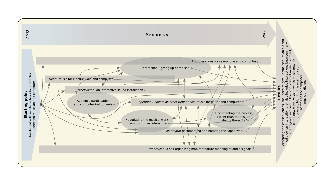
\includegraphics[width=\textwidth]{img/map8-noheader}
  \caption{A timeline with the different sub-projects and themes with their interrelations.}
  \label{fig:main-map}
\end{figure}

% \section{Project background}
% \label{sec:research-question}

\hypertarget{sec:target:introduction-1}{I do not believe} that art is created in solitary confinement but is nurtured in social, human and cultural interaction. Whether my background as a jazz musician and improviser is the explanation for, or a consequence of, this conception holds no real significance for the reading of this book but there is an interesting connection between the sensibility required by an improviser\footnote{Here, I mean the kind of sensibility that George Lewis would refer to as \emph{afrological}: improvisation, in which the personal narrative, manifested partly through the ``personal sound'', is of importance but in which the ``focus of musical discourse suddenly shifts from the individual, autonomous creator to the collective - the individual as a part of global humanity''. \cite[See][110]{lewis-1}} and the sensibility required in any human interaction. 

The primary focus of my PhD project is the interaction between \useGlosentry{glos:musician}{musician} and computer within the context of what is often referred to as \emph{Interactive Music}.
\footcite[See][]{wiki_interactive,Garnett,rowe,winkler01,rowe01} Though this is a commonly used term its meaning is blurred by the magnitude of the concepts that it covers and, in order to unwrap the idea of \index{interaction!musical}musical interaction with a computer, this project also includes other forms of interaction in different contexts and between other kinds of agents as well as different readings of the idea of interaction. These investigations are conducted in the form of reflection on both my artistic and theoretical work. As will be seen, the consequences of the experiences gained from my practice as an improviser and composer may in the end change the way an interactive system, in which a computer is one of the agents, is designed, approached and used. Hence, the study of \useGlosentry{glos:musician}{musician}-musician interaction within this project is not a goal in itself but rather a way to approach the complex field of musician-\index{interaction!computer}computer interaction, which is the type of interaction implied by \emph{Interactive Music}. Similarly, the study of \index{interaction!human-computer}\index{HCI}human-computer interaction is not an end in itself but a way to further understanding of musician-\index{interaction!computer}computer interaction.

%Although human-computer interaction is a very active field of research, its results are not necessarily applicable to the field of art practice. According to interaction researcher Kari \citeauthor{kuutti96} not even software designers are making use of advances in HCI research: ``There is a well-known gap between research results and practical design''.\footcite[18]{kuutti96} \citeauthor{kuutti96} is primarily looking at the interdisciplinary research done in HCI and cognitive psychology and concludes that ``some of the most remarkable new interfaces have been developed with almost no help from research into cognitive psychology''\footcite[18]{kuutti96} If the primary targets for HCI research---interface designers and software developers---are not finding use for it, what is in it for the arts?\footnote{I should remark that a lot has happened in the ten years that has passed since \citeauthor{kuutti96} wrote this article and the surveys and references quoted are almost 20 years old.} The question of the relation between human-computer interaction and the field of art, that is, the question regarding the possibility for a mutual exchange and benefit, will be discussed in more detail in \hyperlink{par:inter-defin:3}{section \ref*{sec:inter-defin}}. Though there are obvious similarities---both are concerned with humans interacting with computers---there are equally obvious dissimilarities.

%This is obviously not to say that HCI research is useless---on the contrary---it is a very important research field with an ever increasing number of applications. But, what is HCI? What does it mean to interact with a computer?

\section{Personal background}
\label{sec:personal-background}

\begin{wrapfigure}{l}{0.15\linewidth}
  \centering
  \includegraphics[width=0.5\linewidth]{img/map9-starting-point}
  \label{fig:starting-point}
\end{wrapfigure}

I have two principal areas of interest in my musical practice: improvisation and computers.
\noindent (\emph{i}) As a performer I look at different ways to explore improvisation: idiomatic (primarily jazz) as well as non-idiomatic,\footcite[The terms, `idiomatic' and `non-idiomatic' are borrowed from Derek Bailey. See][]{bailey92} pre-structured and without preparation (as little as is possible), on acoustic instruments and on electronic and home made instruments (mostly \index{software}software instruments on laptop). Even when working with composition in a relatively traditional manner (i.e. using musical notation), I am always looking for ways to allow improvisation to form an integral part of the process. 
At the risk of provoking the controversy about the difference between improvisation and composition,
\footnote{Whether they are part of the same process or different modalities all together depends on whom you ask. Bruno \citeauthor{nettl74} dismantles the composition-improvisation dichotomy replacing it with the idea of points along a continuum. \parencite{nettl74} Towards the end of his influential book on improvisation Derek \citeauthor{bailey92} quotes a discussion in which it was established that ``composition, should there be such a thing, is no different from composition''. \parencite[140]{bailey92} Finally, Bruce Ellis Benson describes improvisation as a property of all musical practices, even composition. \parencite{benson03}} 
%\footcites(Whether they are part of the same process or different modalities all together depends on whom you ask.)()[Bruno Nettl dismantles the composition-improvisation dichotomy replacing it with the idea of points along a continuum.][]{nettl74}[Towards the end of his influential book on improvisation Derek Bailey quotes a discussion in which it was established that ``composition, should there be such a thing, is no different from composition''.][140]{bailey92}[Finally, Bruce Ellis Benson describes improvisation as a property of all musical practices, even composition.][]{benson03}
I must state that in my experience improvisation precedes composition. Composition appears to me to be a more specialised subclass of the practice of improvisation.\footfullcite[These ideas seem to be getting some support from the aforementioned][]{benson03} This relation is also noticeable with regard to \index{interaction!computer}computer interaction, as the strategies I have developed for dealing with the computer's shortcomings\footnote{The computer's shortcomings are dealt with in the chapter on interaction.} while composing do not usually apply to the case of performing, and certainly not to improvising with the computer. Should interaction in the real-time context of improvisation develop and allow for more enunciated dynamics, this would unequivocally inform---and render different---non real-time work such as composing.

\noindent (\emph{ii}) We are constantly surrounded by technology, technology to help us communicate, to travel, to pay our bills, to listen to music, to entertain us, to create excitement in our mundane lives, etc. For the most part, most users are blissfully unaware of what is going on inside the machines that produce the tools we use (the machine itself is usually much more than the tool). There is no way to comprehend it experientially---it is an abstract machine (though not so much in the Deleuzian sense). If a hammer breaks we may reconstruct it on the basis of our experiences of using it but if a computer program breaks the knowledge we have gained from using it is not necessarily useful when, and if, we attempt to mend it. This phenomenon is not (only) tied to the complexity of the machine but is a result of the type of processes the machine initiates and the abstract generality in the technology that implements the tool.\footnote{The abstract Turing machine, the Mother of all computers, is generally thought to be able to solve all logical problems.} I have worked with the computer one way or another in almost all of my artistic work since 1994 and I am still as fascinated by it as I am by the piano or the saxophone. Whereas the piano and the saxophone are already `owned' by music, however, the computer is not. It is subject to constant change and, even though the computer is obviously already an integral part of our culture and a part of our artistic explorations, the speed with which new and faster technology and new technological tools are produced constitutes an unprecedented challenge to anyone interested in incorporating and understanding computers in the frame of a culture that normally proceeds at an entirely different pace. For exactly these reasons, however, I feel a growing responsibility also to explore the computer for artistic purposes---if only to counterbalance the otherwise purely economical considerations surrounding the development and implementation of new computer-based technology. 

My interest in integrating and interacting with electronically produced sounds began in the late 1980s when listening to saxophonists such as Gary Thomas\footcite{thomas88} and Greg Osby
\footcite{dejohnette88} using the IVL Pitchrider\footnote{The IVL Pitchrider is now out of production. At its time it was a state of the art pitch-to-MIDI converter. It took an audio signal from a microphone and sent out a \useGlosentry{glos:MIDI}{MIDI} signal that could be used to control a synthesiser.}, and Frank Zappa playing the Synclavier.\footcite{zappa86,wiki_synclavier} Pat Metheny's use of guitar synthesiser and sampler on the \emph{Song X} record with Ornette Coleman was a thrilling sonic illustration of what could be done relying on what today we would call relatively simple technology.\footcite{metheny86} Later, hearing George Lewis's \emph{Voyager}\footcite{lewis92} I realised the possibilities for something else than the one-to-one mapping between the instrument and the electronics used in the examples above,\footnote{To be honest, it was only when listening to the track \emph{Traf} on Gary Thomas's \emph{Code Violations} that I started thinking about different mapping schemes: ``I assigned a different harmony note to each note I play on the saxophone; I set it up the way I prefer to hear notes run together''. In the same text Thomas makes another interesting remark that had a big impact on me: ``You can take the limitations of tracking technology and turn them into advantages: if you bend a note on the sax, the synth note doesn't bend, so you get some dissonances''. The idea of using the limitations of technology to one's advantage is a way of soft-circuit-bending; using technology in ways and with methods they were originally not intended for. \cite[See cover notes in][\textparagraph 7]{thomas88}} \hypertarget{sec:target:personal-background-1}{described by} \citeauthor{lewis00} ``as multiple parallel streams of music generation, emanating from both the computers and the humans---a non-hierarchical, improvisational, subject-subject model of discourse, rather than a stimulus/response setup''.\footcite[34]{lewis00}

In the early 1990s I was not attached to any academic music institution and I had no computer science training or knowledge. What started at this time was a long process of \emph{reverse-engineering} the sounds I had heard and the processes I was interested in, in the total absence of a terminology or even a language in which to express what I wanted to achieve. The only method available to me was trial and error. In a sense, this book, along with the website\footnote{See \url{http://www.henrikfrisk.com/improvisation.}} is the collection of information, reflection, and documentation that I would have liked to have had access to while taking my first steps in \emph{Interactive Music}. In hindsight I can see that a lot of material, experience and expertise existed but my lack of knowledge and terminology, in combination with my personal and artistic preconditions, made it necessary for me to begin by finding out by myself.

Ten years later I had acquired the knowledge and the expertise to do many of the things I had targeted. Although, however, I was working actively as an improviser and composer with interactive music in different contexts, and though I was able to stage performances with a comparatively high degree of real time interaction between \useGlosentry{glos:musician}{musician}(s) and computer(s), I was not convinced by the \emph{interactive} aspect of the music. In one sense the music was interactive; I used little or no pre-prepared material and many aspects of the shaping of the computer part were governed by performance time parameters, but in another, perhaps more musical, sense it was not interactive at all. At the time, my identification of the source of dissatisfaction was the fact that the information transmitted from musician to machine, once it arrived at the destination in a machine readable format, was no longer of a kind relevant to the music. The information may still have been valid at the source, but when the representation of it was used in the machine to produce sonic material, material that would appear for the musician as a result of the input, the perceptual connection between cause and effect had been lost and with it, I felt, some of the motivation for working with interactive music. One may object to the conclusion that lack of musical relevance of the \emph{signal} at the destination is a problem, arguing instead that the problem is related to a dysfunctional \emph{use} of that signal at the destination. At the time, however, I was convinced that no matter how sophisticated the mapping between input and output would get, or how cleverly the input signal was used, if the extracted information was not meaningful in relation to the way the music was constructed, the interaction as \emph{interaction} would fail (which is not to say that the music would necessarily fail). 

\begin{figure}[ht]
  \centering
  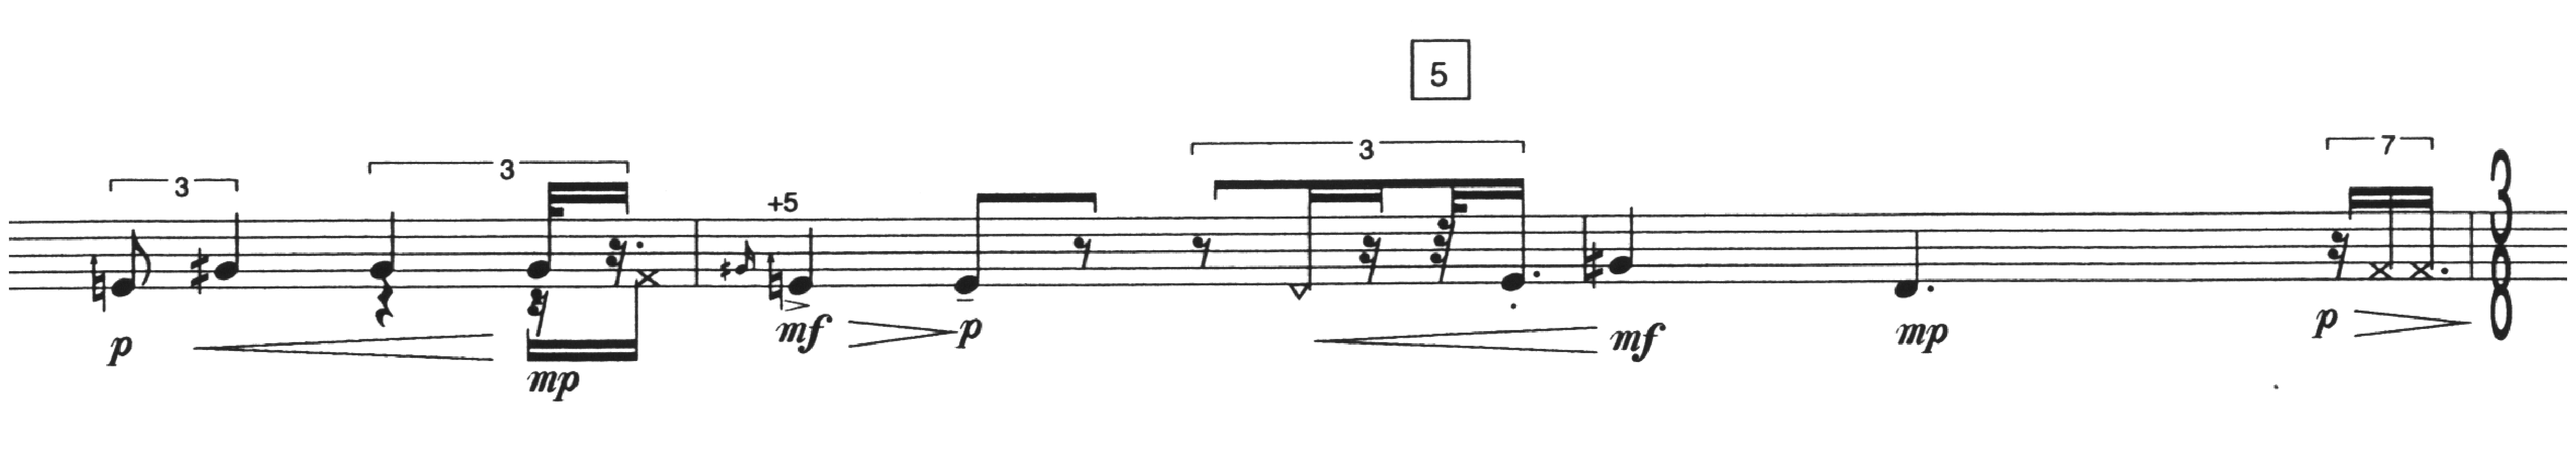
\includegraphics[width=\textwidth]{img/goda-onda}
  \caption[Score excerpt from \citetitle{goda-onda}.]{Score excerpt from the piece \citetitle{goda-onda} by the author. Published by dinergy music pub. \& Svensk Musik}
  \label{fig:goda-onda}
\end{figure}

\hypertarget{sec:target:personal-background-4}{The score excerpt} in Figure \ref{fig:goda-onda} shows bar 3--5 of the flute part of the piece \citetitle{goda-onda} for flute and computer,\footcite[][]{goda-onda} composed 1998/99, and may be used to illustrate one aspect of the problem described above. The piece uses \useGlosentry{glos:pitch-track}{pitch-tracking}\footcite[The pitch-tracking is achieved with the \emph{fiddle\~} object in \index{Max/MSP}Max/MSP. See][]{puckette98} and \index{score following}score-following techniques\footcite[For an overview of \index{score following}score-following techniques, see][chap. 3.2]{rowe} to synchronise the computer with the performer. Overall, in \citetitle{goda-onda}, the \useGlosentry{glos:score_follow}{score-following} works well and is relatively predictable and because the piece is essentially modal, largely owing to the way the modes are composed, the extensive use of micro-tonal variations (e.g. the recurring G quarter tone sharp in the excerpt) does not present a problem. Instead, the issue is the discrepancy of the role pitch has in the structure of the piece on the one hand and in the computer system on the other. Despite the modal nature of the piece, the overriding principle in \citetitle{goda-onda} is not pitch, but rather the way pitched content is combined with non-pitched content, or `regular' flute-sounding notes with ``non-regular'', but what is communicated to the computer is merely the former half of that relation (which in this case is less than half of the information). For example, in the second bar of the note example, the last note, an E (to be played $5/100$ of a tone sharp) is preceded by a D played as a flute pizzicato. Compositionally the `meaning' of the E lies in its relation to the preceding pizzicato tone D and the `meaning' of the D is much more closely related to its timbre than its pitch (which may or may not be a D). None of this information, however, is made accessible to the computer, which is merely receiving information about when a tone is played and what its pitch is.\footnote{In this particular example it may be argued that, if the \index{score following}score-following is functional, information \emph{about} a note (timbre, loudness, articulation, etc.) could be derived from the score rather than the performance. So long as the performance is synchronised with the score, all the information about a given note is (in some cases thought to be) part of the score. \citetitle{goda-onda}, however, contains substantial sections of improvised material where this meta-information is not available prior to performance time. In other words, even if a score-centric (as opposed to performance centred) view is desirable---which it is not to me---it would not work in this composition.} \hypertarget{sec:target:personal-background-2}{Here I located} the source of my frustration: in the computer-performer communication I was limited to one kind of information and that type was not really relevant to the processes I wanted to perform (musically and technically). I saw the solution to this, and other similar problems, in the concept of tracking the timbre, or the relative change of timbre in addition to tracking the pitch.

%; to extract information from the performance of a kind less specialized than pitch only.

If what is described above was the point of departure for this project, although I now more or less have the tools that constitute the first step towards allowing timbre tracking, I have also learned that the problem as described with regard to \citetitle{goda-onda} was badly stated in the sense that it saw the problem, as well as its solution, in far too narrow a way: as a computational task that `only' needed its algorithm. During the course of the project the view on interaction has been broadened to include aspects of interaction that are external to the field of \index{interaction!human-computer}\index{HCI}human-computer interaction. The two main reasons for this may be very briefly summarised as:
(\textit{i}) first of all, interactive music is obviously contingent on kinds of interaction that are not related to the computer. Hence, what is perceived as a dysfunction pertaining to the interactive computer system may under certain conditions be resolved by compensating for it somewhere else, i.e. not necessarily in the computer system itself.
(\textit{ii}) \hypertarget{sec:target:personal-background-3}{second}, regardless of the kind of interaction at work, the attitude towards it and the expectations from it are attributes that consciously or unconsciously shape the design of an interactive system. It is clear that if I expect to be able to \emph{control} an interactive computer (music) system and I fail to do so, I am likely to deem the interactive experience unsatisfactory. From an artistic point of view, however, I will also need to ask myself if expectation of \emph{control} is at all desirable.
In other words, the project started from a relatively narrow view on interaction only to gradually expand it, but without losing the original ambitions, though these would gradually also appear in a new light. The ways in which it expanded, as well as the reasons for the expansion, will be the subject of the following chapters.

\section{The field of research}
\label{sec:summary}

The current PhD project marks an important step in the work in progress for which the goal may be summarised as: to be able to interact dynamically with computers in performances of improvised as well as pre-composed music. `Dynamically' should be understood as non-static in the moment of performance, i.e. \index{real-time}\index{time!real-time}real-time dynamic, but also dynamic with regard to context in non \index{real-time}\index{time!real-time}real-time, as a multiplicity of possibilities: to resist the notion of \emph{the} solution, to defy the \emph{work}, and constantly to re-evaluate and transform according to the changing needs: to opt for the \emph{work-in-movement}. The latter understanding of `dynamic' is furthermore the origin of the concept of re-evaluation of `the \index{Self}Self' that has become central to this project: When 
%the particular solution is dissolved and 
others are allowed entry into the constructive and defining phases of a musical work (which is the consequence of the decomposition of \emph{the work} and the beginning of the \emph{work-in-movement}), the \index{Self}Self of musical production is likewise to be questioned. The significance of these issues was not originally part of the project but was revealed to me while I was working on the \hyperref[sec:ethersound]{interactive sound installation \emph{etherSound}}. As a sound installation it dismantles the relationships between composer, performer and listener. (In relation to \emph{etherSound}, am I the composer, the performer or the listener? Attempting to define one's role, however, is the sign of a relentless articulation of the \index{Self}Self.) Out of these contemplations, in combination with the experiences of audience interaction and participation also gained from \emph{etherSound}, came the notion of \emph{\index{interaction!as difference}\index{interaction-as-difference}interaction-as-difference} as opposed to the common mode of \index{interaction!human-computer}\index{HCI}human-computer interaction, defined here as \emph{\index{interaction!as control}\index{interaction-as-control}interaction-as-control}. 
%In other words, how may the concept `giving up the self' as the first step of human-human interaction on equal terms, and as a possibility for rethinking my musical practice, also be applied to human-computer interaction, in the context of production of musical content?

In this project the (artistic) practice is, in a sense, both the object and the method. The sub-projects contained within the frame of this thesis, some of them still works-in-progress, are used to make inquiries into the larger question of the significance of interaction in the context of artistic practice involving computers. As mentioned above, they are manifestations of different modes of interaction and as such they form the basis for reflections on the subject. Hence, though there are a number of aspects on interaction in relation to computers, musical practice, improvisation and many other topics that could have been followed up, the artistic work has been the proxy that has helped to demarcate and narrow the field of questioning. I should however mention, albeit briefly, one currently influential field that is \emph{not} actively discussed in the present work, but which is very closely related to it. The field of gestural control of music,\footcite[For an overview, see][]{wanderley00} has attracted a great deal of interest within \index{digital}digital media in general and \index{electro-acoustic music}electro-acoustic music in particular in the last decade and includes concepts such as embodiment, immersion and body-sound interaction.\footcites(In the early and mid-1990s \index{virtual}Virtual Reality technology, also in artistic practice, was a source of inspiration for thinking about the role and function of the body in human-technology interaction as well as concepts such as immersion.)()[See][]{moser96}[see also][]{wood98} With no intention of presenting a complete list, I could mention related projects---projects that also share a strong connection to artistic practice as well as to improvisation and/or technology---such as those by pianist and improviser Vijay \citeauthor{iyer08}\footcites[See the PhD thesis][]{iyer98}[See also][]{iyer08} and the saxophonist David \citeauthor{borgo05}.\footcite[Using British saxophonist Evan Parker as a point of demarcation the embodied mind is explored in][chap. 3]{borgo05} They are both examples of improvisers/researchers with a great interest in the study of music and improvisation as an embodied activity. In addition, Norwegian ``music researcher and research musician''\footcite{jensenius08:bio} Alexander \citeauthor{jensenius08}'s recent PhD thesis is a project intimately tied to the author's artistic practice, similarly focused on embodied music cognition and on gesture control of electronic musical instruments.\footcite[See][]{jensenius08}

% In Section \ref{sec:interaction} I will discuss \emph{Interaction} in
% general and then, in Section \ref{sec:interactive-music} I will look
% at that which is commonly referred to as \emph{Interactive Music}.
% That being the meta-level of interaction, I will then proceed to
% discuss the micro-level, the code, or the language and the processes
% of signification---and its nature and quality---and if that may or should
% be considered in interactive music.

%Though this thesis certainly marks the end of one phase, it most certainly, for me personally, also marks the beginning of another.

\newpage
\section{Sub-projects---overview}
\label{sec:overview}

\begin{figure}[!ht]
  \centering
  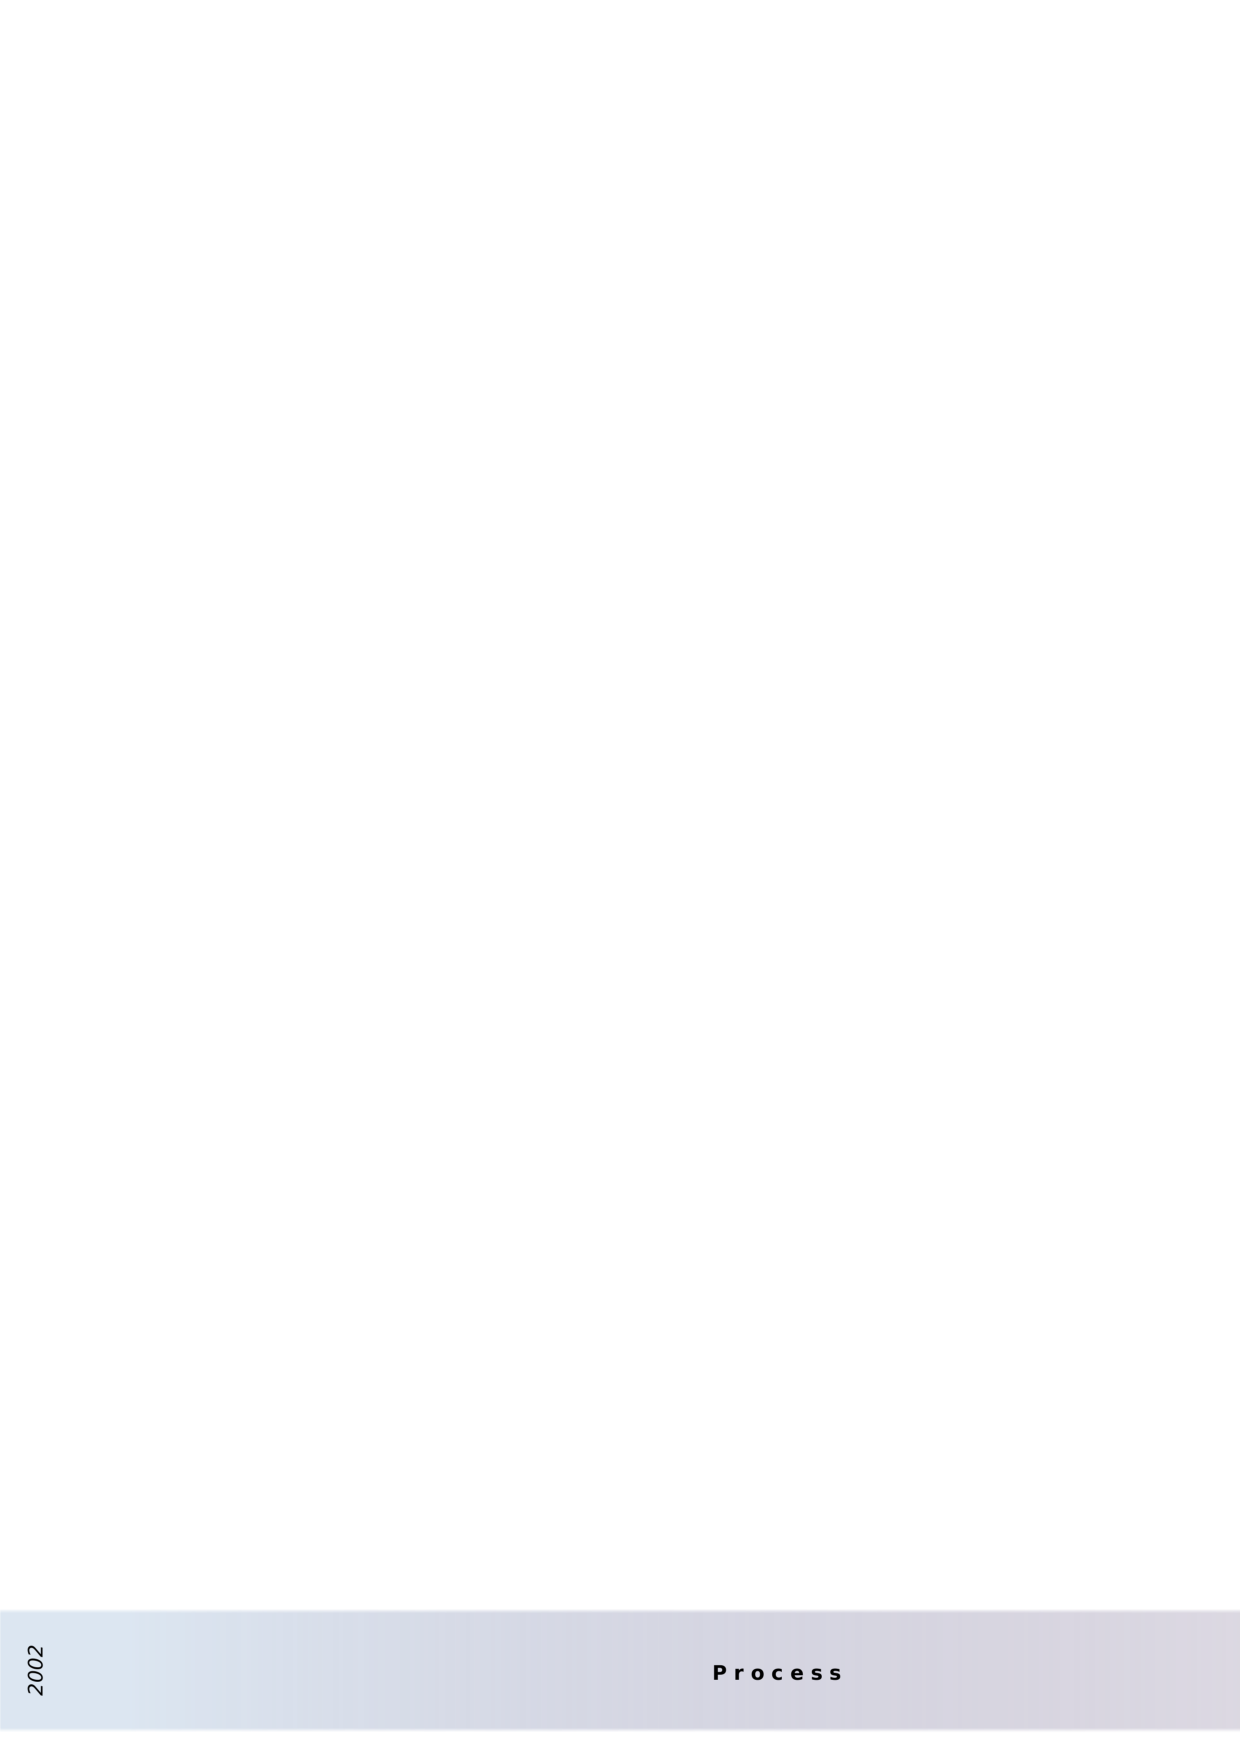
\includegraphics[width=\textwidth]{img/process}
  \caption{Process arrow of project map (See Figure \ref{fig:main-map})}
\end{figure}

This section is intended to function as an annotated table of contents for the reader to get an overview of the project but also to allow for reference look-up of particular components. Although I prefer to see all aspects of this project as a distribution of interrelated parts that overlap with each other, all belonging to my artistic practice, in order to unwrap and make accessible the different facets of import to the thesis, a dissection, so to speak, is necessary. Graphically displayed in \hyperlink{fig:target:main-map}{Figure \ref*{fig:main-map}}, the different enclosures, or sub-projects, are briefly introduced below, but the enclosures are also carriers of artistic experience and have in themselves something to say about the subject matter. The different modes of interaction represented in these artistic projects are not only relating to musician-\index{interaction!computer}computer interaction but also in high degree to musician-musician interaction: interaction taking place in the stages of preparation and development of the projects as well as in the processes of performance, execution and evaluation. Below, the projects appear roughly in the order in which they were initiated in time, but it should be noted that they also extend over time. For example, though \emph{timbreMap} was the first sub-project started, it is also the one that has been active the longest. Although it would be possible to categorise the different sub-projects into `music', `text' and \index{software}`software', in the presentation below I have not done so because I believe it would give a wrong picture of the types of works included here. By resisting this categorisation I hope also to resist the corresponding division of sub-projects into `artistic', `reflective' and `scientific' solely on the basis of their \emph{form}. It is not that I think my music is scientific or my programming is reflective but nor do I think my texts are \emph{only} reflective. For instance, the computer \index{software}software which is part of this project is not merely a ``tool'' to allow for ``testing'' or ``verifying''. I regard it as part of the artistic practice that lies at the very foundation of this project, i.e. as implementations of ideas. They are also beginnings in themselves, however, in that they may, albeit in a limited sense, allow for a different usage of computers in the context of interactive music.

The purpose here is not to draw conclusions that may be \emph{generalised} but rather to test assumptions within the framework of my own artistic production. The \index{software}software, released under the \citetitle{GNUGPL},\footcite{GNUGPL} as well as the music,\footnote{I am currently investigating the consequences of releasing all, or much of my music under the \citetitle{CCLIC}. See \cite{CCLIC}.} may very well be used in other contexts, by other artists for completely different purposes, or to elaborate on the ideas presented in this book. Though programming as an activity is often seen as something done by predominantly asocial men, in isolation, I argue that programming is interaction. It is interaction in order to make the computer interactive, interaction in the language of the computer, but these projects, notably libIntegra, are also in themselves results of higher-level interactions as in group collaboration.\footnote{I would go so far as to say that, based on my own experience, the interaction between myself and Jamie Bullock (the main \index{software}software developer and administrator of the project) was a critical aspect of the development. As the project involved many low level decisions that could potentially be highly significant at a much later stage, there were at times very intensive communication and negotiation between us that in most cases led to new ideas and input in the project. In that sense the interaction was more important than the development.} Many open source \index{software}software development projects interact widely with their users, other developers and other projects.

\hypertarget{sec:target:overview-1}{The computer}, as a physical object (as opposed to the abstract \emph{idea} of the computer), is often intimately coupled with the \index{software}software it hosts, to the degree that operations that are a result of \index{software}software processes are attributed to the computer as object rather than the actual program in question. Furthermore, it is imaginable that, in some cases, these operations should more correctly be associated with the programmer rather than the program. For example, when playing chess against a computer chess program, one has the sensation that the game is played against the \emph{computer}, when in fact the game is played against a dislocated chess game \emph{programmer}.\footcites[See J. Gilmore as quoted in][]{arendt77}[See also][]{baudrillard02:blue} \hyperlink{sec:target:human-comp-inter:par3}{In Section \ref*{sec:human-comp-inter}} the computer operating system is discussed in similar fashion as a sign referring back to the producer of the system. If we can talk about signification in this context the \index{software}software is the sign that holds a causal relation to output of the program, which in turn signifies the origin of the program: the programmer(s) or the context s/he or they belong(s) to. Now, this is not a general clause. To delineate \index{software}software and talk about it as a symbol somewhat independent of its host in this manner is obviously not always possible: compilers and embedded systems are only two examples. In my own practice, however, the idea that programming is a means of positing some part of myself within the \index{software}software, not unlike how writing a musical score is a way to communicate oneself, has become an important aspect. Under certain conditions, the computer, when running \index{software}software I have contributed to, may then be seen to function as a mediator of myself, again similarly to the way a score is a mediator of its composer. The computer acts as a host for a detached \index{Self}self, as an `instantiator' of my imprint, the code, with which I can interact. Contrary to the immediate appearance of ego-centric narcissism in this description---coding the \index{Self}Self to play the \index{Self}Self to interact with the \index{Self}Self---for me, the \index{Self}Self is instead distorted. (Under certain conditions the result could equally well turn out to manifest narcissism.) In the superimposition of different kinds of logic, of \index{Self}Self as sign and \index{Self}Self as \index{Self}Self, and different kinds of time, that of real time and that of detached time, a possibility for losing the \index{Self}Self eventuates.
\newpage
\subsection{timbreMap}
\label{sec:timbremap}

\begin{wrapfigure}{r}{0.4\linewidth}
  \begin{minipage}[h]{\linewidth}
    \begin{flushright}
      \musicannot{timbreMap\\
        \emph{demonstrations of real time self-organisation}}
    \end{flushright}
  \end{minipage}
\end{wrapfigure}

%%% Local Variables: 
%%% mode: latex
%%% TeX-master: "../ImprovisationComputersInteraction"
%%% End: 


To be limited to pitch-tracking as input source in my saxophone-computer interactions\footnote{Naturally, other options exist and any number of combinations of existing solutions for instrument-computer interaction is possible. My point here is that, for different reasons including the fact that pitch is quantifiable, pitch-tracking has become a very common mode of interaction.} has for long appeared to me like trying to paint a picture on a computer screen with nothing but a computer keyboard to do it with, or, the reverse, to try to type a letter with nothing but a joystick. Ultimately trying to compensate for unwanted artefacts when transgressing the barrier between continuous and discrete becomes too annoying. The concept of \useGlosentry{glos:pitch-track}{pitch-tracking} was briefly \hyperlink{sec:target:personal-background-4}{discussed above} in connection with \citetitle{goda-onda}, a composition which also provided a practical example of the possible limitations with pitch-tracking in instrument-\index{interaction!computer}computer interaction. What the process of pitch-tracking attempts to achieve is the transformation of a (monophonic) audio signal into a series of discrete pitches.\footnote{As mentioned, \citeauthor{puckette98} (\citeyear{puckette98}) describes the \emph{fiddle\~} Max \& Pd object which uses a frequency domain method to estimate the pitch. Another option to extract the pitch from an audio signal used sometimes is \emph{zero-crossing}, in which the signal is analysed in the time domain. \cite[For an example, see][]{cooper94}.} Aside from the fact that pitch-tracking is a difficult task, the information gleaned by such systems is only useful if the pitch representation is a meaningful and substantial parameter in the intended totality of the musical output. In much of my music it is not. I am primarily interested in the non-quantifiable aspects of the audio signal such as timbre and loudness and, although it is entirely possible to create continuous change from discrete events, it appears more natural to me to make use of the continuity already present at the source (the saxophone) than to recreate it from a quantised event. If this were possible, I imagine the chances for the two sounds to integrate, to blend, would increase.
%This, I should point out, is related to my personal predisposition for hearing and not a general clause.
The \emph{timbreMap} \index{software}software is an attempt to assess the hypothesis that this relation between the nature of the signal used as input in the musician-\index{interaction!computer}computer interaction and the nature of the output is of importance. In this sub-project I am addressing the problem defined at the outset, described towards the end of \hyperlink{sec:target:personal-background-2}{Section \ref*{sec:personal-background}} and also below in \hyperlink{sec:target:music-pract-inter-1}{Section \ref*{sec:music-pract-inter}}, namely the question of the role of timbre in musician-\index{interaction!computer}computer interaction: will information about the relative timbre in an audio signal make possible a different type of interactive system, one that can more easily achieve sonic integration? Before we look at the proposed system itself, the issue of integration, or `blend', needs to be unwrapped. 

One of the great challenges of working with \index{electro-acoustic music}electro-acoustic music in combination with acoustic instruments is how to unite the two sound worlds into one coherent whole. This statement, however, brings forth a number of questions such as why a coherent whole is important.\footnote{Electronica, techno and lots of other popular music styles, as well as much \index{electro-acoustic music}electro-acoustic music, thrive on their sonic space being distinct from the acoustic sound world of traditional instruments.} Further, what does it mean for two sounds to unite? To begin with, the lack of physicality, the absence of a body, in \index{electro-acoustic music}electro-acoustic music production is an issue. If two human musicians are playing together before an audience, their mere being there together, their physical presence, will contribute to making the listener unite the timbres. If one of the musicians is instead a virtual one, a computer, though there is the advantage of near limitless sonic possibilities, there is the disadvantage of having to create the sonic unity with sound only.\footnote{The topic of sound and physicality is huge and obviously not done justice by this short and rather simplistic example. As a field of research it is related to the topic of embodiment and enactment. Apart from the references mentioned in \hyperref[sec:summary]{Section \ref*{sec:summary}}, \cite[see][chap. 1, \ppno 3--30]{gill08}} Now, unity in this context should be understood not only in the holistic sense that the two sounds unite or blend into a whole, but also that the two sounds may in some regard create a perceptual unit. The sonic relation does not have to be one of unity; it may equally well be an antagonistic one, in which case the struggle is the perceptual unity. In other words, the notion of the `blending' of sounds also holds within it concepts such as distortion, noise and power.

In my experience, primarily of the styles of jazz and improvised music---also of conducting, playing in, and composing for, big bands---`blend' is a highly complicated issue. It is not a predetermined factor but a property relative to a large number of agents. Blending is a constant negotiation in which tone colour, intonation, energy, volume, articulation, etc. have to be perpetually altered. The ultimate goal of this negotiation is not unity, but difference---there is nothing as difficult as trying to blend with one's own sound. In this sense, blending is not only a communication of information from one part to another but something which happens `in between'. And, it is the `in between' that remains hidden if the \useGlosentry{glos:musician}{musician}-\index{interaction!computer}computer interaction is not truly continuous. Despite its limited scope, the tests I have performed with \emph{timbreMap} seem to show that it is capable of communicating information of a kind useful in the attempt to achieve `blend'.

\subsubsection{The design}
\label{sec:timap-design}

\emph{timbreMap} makes use of a \index{self-organising map}self-organising feature map (SOM) of the type proposed by Teuvo \citeauthor{kohonen88} which provides a two dimensional topographic map of some features in the input vector. A \useGlosentry{glos:som}{SOM} is a type of \index{Artificial Neural Network}\index{ANN}artificial neural network (ANN) and, apart from \citeauthor{kohonen88}'s phonetic typewriter, has been used for a wide range of purposes.\footcite[See][137--40]{gurney97} In general there has been interest for many years from the \index{electro-acoustic music}electro-acoustic music community in ANN. The MAXNet object that ``simulates multi-layered feed forward and Jordan and Elman style recurrent networks'' was made available for the \useGlosentry{glos:Max}{Max} graphical language for audio and \useGlosentry{glos:MIDI}{MIDI} processing in the early 1990s.\footcite{wessel91} Robert \citeauthor{rowe} has a section on \useGlosentry{glos:ann}{ANN} in his book \citetitle{rowe}\footcite[chap. 7]{rowe} and \citetitle{miranda99} has several contributions that relate to the subject.\footcite{miranda99} The recent interest in ecological thinking,\footnote{In ecological thinking, perception and meaning are coupled.} also in music, has made connectionist ideas spread outside the confines of computer science. In ecological thinking the environment is structured and the perception is flexible; to perceive is to become attuned to the structure inherent in that which is perceived. Musicologist Eric \citeauthor{clarke05} describes the kind of attuning ``to the environment through continual exposure'' that briefly summarises the behaviour of a SOM as a result of the plasticity of perception and actually proposes that connectionist models are approached for greater understanding of aspects of the human capacity for self-organisation.\footcite{clarke05} \emph{timbreMap} depends on the highly flexible and efficient JetNet FORTRAN library implementation of SOM.\footcite{lonnblad91}

The original design of \emph{timbreMap}, written in C++, loosely follows a model for speaker independent word recognition suggested by \citeauthor{huang92}.\footcite{huang92} It constructs its input vector by performing a Bark scale transform which divides the signal up into twenty four critical bands. These are derived to approximate the psycho acoustical properties of human auditory perception.\footcite[See][]{bladon86} The filter curve for the Bark transform used in \emph{timbreMap} is:\footcite[Following][32--3]{bladon86}
\begin{equation}
  \label{eq:4}
  10log_{10}B(z) = 15.81+7.5(z+.474)-17.5(1+(z+.474)^2)^{1/2}dB
\end{equation}
where the bandwidth, $z$ for frequency $f$ is derived from: 
\begin{equation}
  \label{eq:5}
  z=26.81\frac{f}{(1960+f)}-0.53
\end{equation}

\emph{timbreMap} has native support for \index{Open Sound Control}\index{OSC}Open Sound Control ((\useGlosentry{glos:OSC}{OSC}) and interfaces with \hyperref[sec:libintegra]{\emph{libIntegra}} as a stand-alone module. It currently uses Jack\footcite{davis08} for audio input. There is no release of \emph{timbreMap} for it is in a state of constant flux but the source code is available from \url{http://www.henrikfrisk.com}. Among the things I am planning for the next phase of development is adding additional layers of networks, some of which may be supervised learning networks. \emph{timbreMap} is a central component of my more recent saxophone/computer improvisations and of the third version of \emph{Repetition Repeats all other Repetitions}. With it I will be able to inform the computer of relative changes in timbre and this, I hope, will allow me to expand on the possibilities for \useGlosentry{glos:musician}{musician}-\index{interaction!computer}computer interaction.

\newpage
\subsection{Solo improvisations}
\label{sec:solo-impr-2002}

\begin{wrapfigure}{r}{0.3\linewidth}
  \begin{minipage}[h]{\linewidth}
    \begin{flushright}
      \musicannot{Improvisations\\
        \emph{ for saxophone and computer}\\
        Performed in 2005}
    \end{flushright}
  \end{minipage}
\end{wrapfigure}

%%% Local Variables: 
%%% mode: latex
%%% TeX-master: "../ImprovisationComputersInteraction"
%%% End: 


In \hyperref[sec:personal-background]{Section \ref*{sec:personal-background}} I stressed the importance of improvisation in my artistic practice and, with a reference to \citeauthor{benson03},\footcite{benson03} pointed to how experiences gained within the field of improvisation may be of a kind more generic than experiences acquired elsewhere in the vast territory of musical practice. The topic of musical improvisation, for a long time neglected by musicology and music theory,\footcites()()[See, for example,][]{lewis-1}[With regard to improvisation all contributions in the collection are of interest, but regarding the scholarly neglect of improvisation in particular, see][]{nettl98:2}[see also the introduction to][]{bailey92} is a complex one and a full scholarly inventory of its significance and meaning could easily be the subject for a separate thesis.\footcite[Although I tend to agree with Bailey that it is doubtful whether it is at all possible to \emph{describe} improvisation (``for there is something central to the spirit of voluntary improvisation which is opposed to the aims and contradicts the idea of documentation''), there are also non-descriptive and non-documenting ways to do this inventory.][\pno ix]{bailey92} Here I will give a short account of my own views on improvisation, if only to contextualise my aims concerning musician-\index{interaction!computer}computer interaction.

In my own improvisatory practice the two central aspects are \emph{sensibility} and \emph{sound}, each of which may be said to be a fundamental aspect of jazz in general. The relation between inter-human sensibility and improvisatory sensibility was briefly mentioned in the \hyperlink{sec:target:introduction-1}{first paragraph} of \hyperref[sec:introduction]{Chapter \ref*{sec:introduction}}. The sociological and cultural dimensions of sensibility of different kinds are covered by George \citeauthor{lewis-1} in his essay \citetitle{lewis-1} and the intra-musical aspect of sensibility is hinted at by George Russel's notion of \emph{intuitive intelligence}.\footnote{George Russel, in a conversation with Ornette Coleman \parencite[see][]{ornette85}, concludes that the reason Coleman and the members of his band are able to start playing, in time, without counting the tunes off is thanks to ``intuitive intelligence'', according to Russel a property of African-American culture. In an interview with Ingrid Monson, Russel returns to intuitive intelligence with the following description: ``It's intelligence that comes from putting the question to your intuitive center and having faith, you know, that your intuitive center will answer. And it does.'' \parencite[George Russel quoted in][154]{monson98}.} Now, \citeauthor{lewis-1} also discusses the aspect of sound in his essay and how the ``personal narrative'' is part of the individual signature of the Afrological improviser summarised by the conception of his \emph{sound}:
\begin{squote}
\hypertarget{sec:target:solo-impr-2002-1}{Moreover}, for an improviser working in Afrological forms, 'sound,' sensibility, personality, and intelligence cannot be separated from an improviser's phenomenal (as distinct from formal) definition of music. Notions of personhood are transmitted via sound, and sounds become signs for deeper levels of meaning beyond pitches and intervals.\footcite[117]{lewis-1}
\end{squote}
The topic of the \index{Self}Self in relation to sound brought up by \citeauthor{lewis-1} will be discussed later but for now let us settle for the conclusion that just by listening to the diversity of expression to be found among jazz musicians it is not difficult to apprehend that `personal narrative' is an important agent in jazz: a genre where the same instrument, played by two contemporaries, could easily show entirely distinct qualities. Now, my point here is not to prove that my improvising shows afrological qualities, but only that I embrace some of the values also assigned to the  afrological ``musical belief system''.

To introduce the computer into the improvisation equation, the interesting challenge is to include it without altering the quality of the coefficients of \emph{sound} and \emph{sensibility}. This is a programming challenge as well as an artistic challenge, and one which poses many questions. What are the essential qualities of sensibility and sound in a context that includes the computer? In what ways may they change? Is something like sensibility at all compatible with the computer? Or even with the \index{digital}digital (as opposed to the continuous)? What is it to prove sensible towards a machine that is insensible by its very nature. Should I alter my own sensibility? Or attempt to alter the computer's capacity for mimicking or responding to sound and sensibility? Or is the human expression so vastly different from the computer's structure that their respective qualities may never be threatened by whatever mode their interaction implements? Going back to \citeauthor{lewis-1}, if sound and sensibility are qualities inseparable from the improviser's empirical understanding of music, what is the effect if this understanding also includes the computer? It is in this context that the \hyperlink{sec:target:personal-background-3}{previously questioned} validity of a control paradigm in musician-\index{interaction!computer}computer interaction becomes significant. 
%These are some of the questions I am concerned with in my solo saxophone and computer improvisations. 

There is a multiplicity of dualities active in this context, dualities that offer resistance, albeit positive ones. The sensible-insensible continuum as well as the analogue-\index{digital}digital dichotomy, but also the \hyperlink{sec:target:overview-1}{duality constituted by the \index{Self}Self} as encoded in the programmed computer versus the \index{Self}Self as ``transmitted via sound'' played acoustically.\footcite[117]{lewis-1} The result of these dualities and their resistances is that the \index{Self}Self is slowly dismantled in a continuous feedback loop that represents a kind of dislocated \index{interaction!human-computer}\index{HCI}human-computer interaction taking place prior to the \index{real-time}\index{time!real-time}real-time, situated interaction. Already asking the questions pertaining to the difference between man and machine is part of a \index{interaction!human-computer}\index{HCI}human-computer interaction and one of the unavoidable outcomes of the dismantling of the \index{Self}Self in this context is the re-evaluation of the central aspects of the practice: in the end the notions of \emph{sensibility} and \emph{sound} may have to be reassessed.

%It is within my work with solo saxophone and computer improvisations that I will be able to assess the particular validity of the study of musician-computer interaction. And it is in this context that I will articulate that which I reach for in interactive saxophone-computer improvisation.

\newpage

\begin{figure}{}
  \centering
  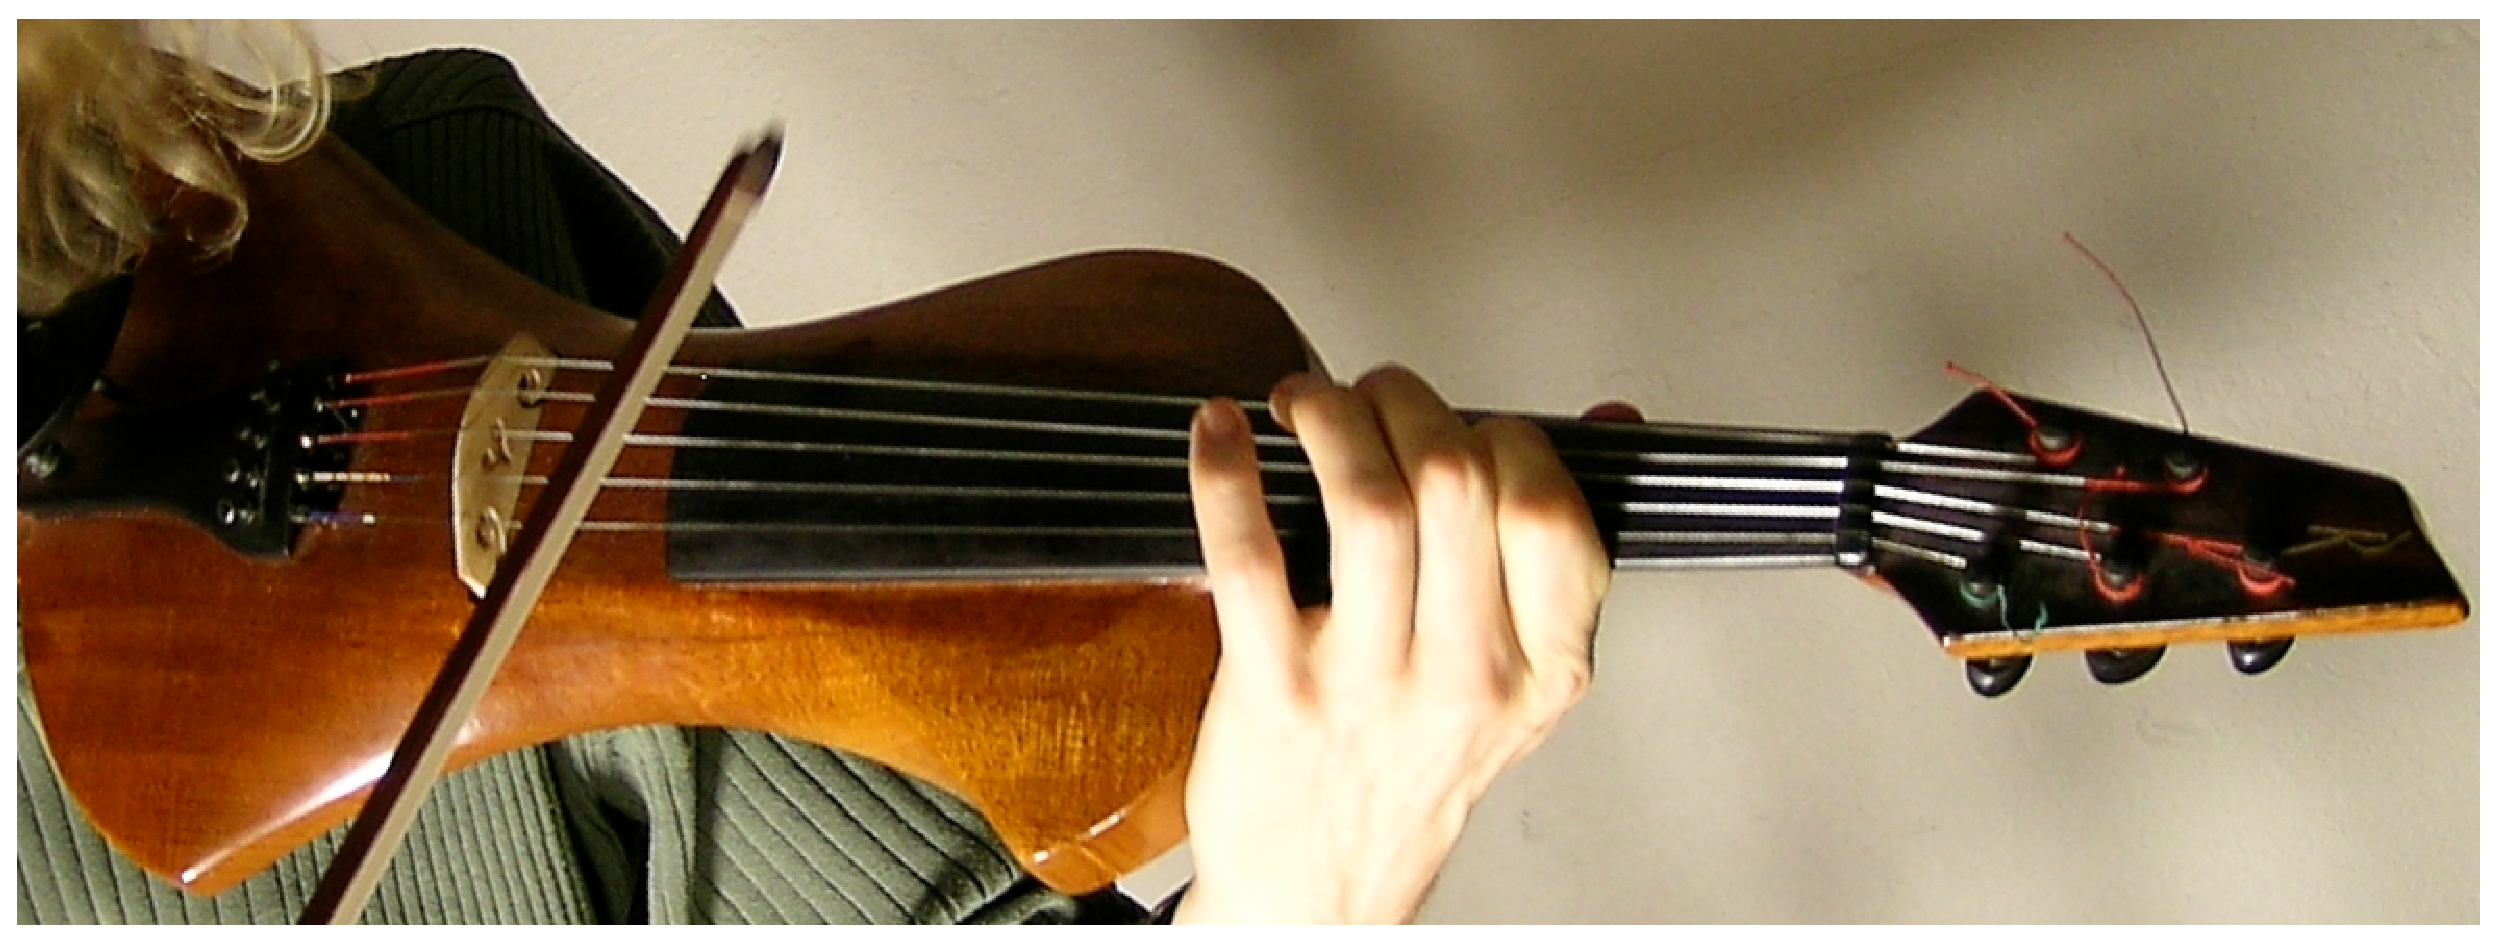
\includegraphics[width=0.4\linewidth]{img/evg-2}
  \caption{The Electric Viola Grande, an electronically amplified viola built by Swedish instrument-maker Richard Rolf.}
  \label{fig:evg}
\end{figure}
%\vspace{1cm}

\subsection{Drive}
\label{sec:drive-2003}

\begin{wrapfigure}{r}{0.45\linewidth}
  \begin{minipage}[h]{\linewidth}
    \begin{flushright}
      \musicannot{Drive\\
        \emph{for Electric Viola Grande and computer}\\
        Composed \& premiered in 2002\\
        Commissioned by and dedicated to Henrik Frendin}
    \end{flushright}
  \end{minipage}
\end{wrapfigure}

%%% Local Variables: 
%%% mode: latex
%%% TeX-master: "../ImprovisationComputersInteraction"
%%% End: 

\emph{Drive} is a composition for \index{Electric Viola Grande}\index{EVG}Electric Viola Grande (EVG)\footnote{The Electric Viola Grande is a custom made, electronically amplified five stringed viola. It was built by Swedish instrument-maker Richard Rolf on commission from Swedish violist Henrik Frendin.}  and computer commissioned by Swedish violist Henrik Frendin for his Phono Suecia recording \emph{Viola con Forza}. \footcite{frendin04} Within the frame of the composition the performer has much freedom to shape the piece in a way that he or she sees fit in order to fulfil the larger structural idea of the composition: a dominant to tonic cadence. The synchronisation between the computer and the performer is achieved by employing the widely used space-bar-piece paradigm:\footnote{I heard this term used for the first time by Sean Ferguson (see \url{http://www.cirmmt.mcgill.ca/People/ferguson}). In the mid 1990s, when it started to become practical to use computers in live performance, a large number of compositions were produced where someone other than the performer(s)---usually the composer---interacted with the computer using the computer keyboard. Each touch of the space bar (or any other key of choice) started the playback of the next pre-prepared sound file or changed the settings (the preset) for an effect or a synthesiser or whatever the next `event' required. It is still a very common mode of interaction in the \index{electro-acoustic music}electro-acoustic music community.} the computer is guided through the different sections of the form of the composition by means of `cues' (pressing the space bar).\footnote{The cue may of course come from any kind of control source from which a clear, noise-free, trigger can be generated such as a pedal pressed by the performer; a uniquely detected pitch in the audio signal; a change of volume; etc.} For every cue (a total of six in the piece) the computer adjusts its internal tempo based on the time lapse since the last cue. In other words, the computer part with its associated `player' and `listener' is progressing at its own pace, occasionally adjusted to the performer's tempo. Although the significance of time in interactive systems will be treated in more depth \hyperref[sec:time-interaction]{in Section \ref*{sec:time-interaction}} the difference between this kind of time based system such as \emph{Drive} implements and a purely event based system should be noted. Whereas the former, in its conception of time, displays some notion of memory or history, though only in a very limited sense, a purely event-based system, with no regard to time, responds to each trigger individually, similarly to how most computer text editors will respond to the trigger \emph{letter `T' pressed} in the exact same way regardless of what came before it, or how synthesiser keyboards respond to the \emph{MIDI note 64} message uniformly disregarding context (see \autoref{fig:serial}). In a very simplistic way the computer part for \emph{Drive} has its own forward motion and its own tempo. It moves in parallel with the performer rather than \emph{only} as a result of a stimulus, and updates its motion and its state according to the cues it receives (see \autoref{fig:parllel}). It is its motion that constitutes its memory and it is the altered tempo that affects subsequent events.

\begin{wrapfigure}{r}{0.55\linewidth}
  \centering
  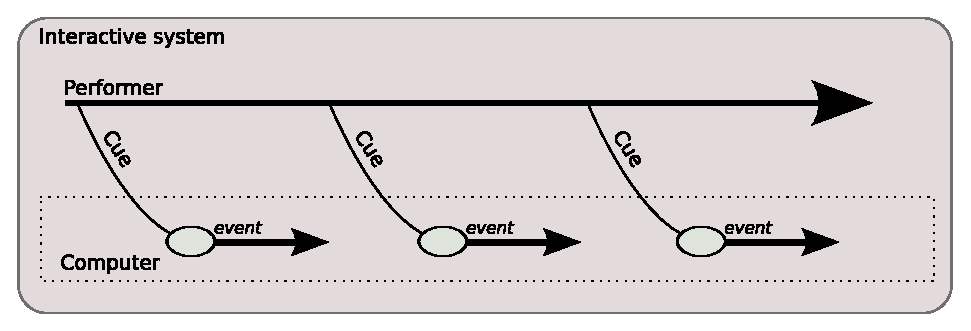
\includegraphics[width=0.95\linewidth]{img/serial}
  \caption[Scheme of a simple interactive system without memory.]{An interactive system with a performer providing the computer (synthesiser, dishwasher, etc.) with singular cues. The (computer) system is agnostic to past cues and events and reacts only to the current or most recent event, i.e. it has no memory as such.}
  \label{fig:serial}
\end{wrapfigure}
Apart from the cues to guarantee synchronisation between the performer and the computer, another more dynamic layer of \emph{harmonic} interaction is active throughout the piece. The computer part resonates with particular frequencies, in terms of both when and how to manipulate the sound of the EVG and when and how to generate new material; a virtual resonance that is used to expand the spectral and timbral range of the instrument. The resonating frequencies are subject to constant change following the composed viola part as well as following the tempo as altered by current and prior cues. Thus it constitutes a sonic layer of communication between performer and computer. If they drift apart in time, there will be less, or substantially different, sonic interaction (an effect the first version of the score already allowed for).

\begin{wrapfigure}{l}{0.55\linewidth}
  \centering
  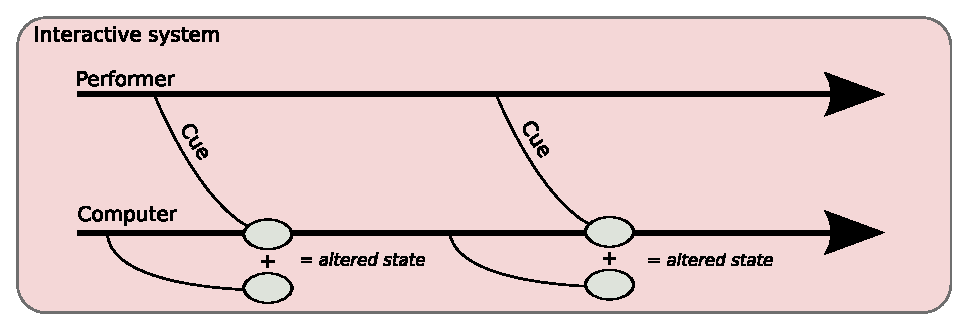
\includegraphics[width=0.95\linewidth]{img/parallel}
  \caption[Scheme of a simple interactive system with memory.]{An interactive system with two players in parallel with a simple implementation of memory. The altered state is a result of the most recent cue \emph{and} past cues and events.}
  \label{fig:parllel}
\end{wrapfigure}
Finally, \emph{Drive} is a composition in which the interaction between myself, as the composer, and Henrik Frendin, as the interpreter, is mediated through an open-ended score. In an ongoing negotiation we each have to question our respective views and personal wishes and open ourselves up to the other's point of view and trust that that view is `genuine'. One result of these negotiations is how the piece was originally conceived of as one that could be played by Frendin alone, that is, without my participating in the performance. Owing to a multitude of factors, however, one being that Frendin preferred me to perform with him, I have taken part in all performances of \emph{Drive}, which has obviously influenced how the piece has developed in the course of the performances and how the idea of interaction has changed from a performer-centred view to a distributed array of interconnected `players'. But it also had more radical consequences that have resulted in a deconstruction (though not so much in the philosophical meaning) not only of the original understanding of \emph{Drive} as a composition (rather than a \useGlosentry{glos:work_in_movement}{work-in-movement}), but of my own role as composer. My performances with Frendin have grown to engendered new positions for both of us. If formerly I assisted Frendin in the `performance of compositions' we now approach our venture with much more distributed roles, hovering in the crevices between composition, improvisation, performance and mixing. Hence, \emph{Drive} initiated another aspect of the dismantlement of the \index{Self}Self possible only if one is \emph{willing} to give up the \index{Self}Self.

Although this project was initiated prior to the studies in \emph{Negotiating the Musical Work}, the project I share with guitarist Stefan \"{O}stersj\"{o},\footcite{frisk-ost06} it nevertheless anticipated certain aspects of collaborative music making, ideas that would later be formalised.

\subsection{etherSound}
\label{sec:ethersound-2003}

\begin{wrapfigure}{r}{0.4\linewidth}
  \begin{minipage}[h]{\linewidth}
    \begin{flushright}
      \musicannot{etherSound\\
        \emph{for improvising musicians, audience and mobile phones.}\\
        Composed \& premiered in 2003\\
        Commissioned by Miya Yoshida}
    \end{flushright}
  \end{minipage}
\end{wrapfigure}

%%% Local Variables: 
%%% mode: latex
%%% TeX-master: "../ImprovisationComputersInteraction"
%%% End: 


\emph{etherSound} is perhaps the most ambitious sub-project. It was commissioned in 2002 by curator Miya Yoshida for her project \emph{The Invisible Landscapes} and was realised for the first time in August 2003 at \emph{Malm\"{o} Art Museum} in Sweden.\footcite[Yoshida's PhD thesis includes a chapter on \emph{etherSound}.][C.5, \pno 165]{yoshida06} Since then it has been performed on several occasions in Sweden, Denmark, the UK and the USA. The principal idea behind \emph{etherSound} is to create a vehicle for audience collaboration in the shape of an `instrument' that is playable by anybody who can send SMS (Short Messages Service) messages. As an interactive system \emph{etherSound} takes input in the form of these SMS messages and creates `message-scores', then transforms them to short electro-acoustic `message-compositions', each one lasting from about fifteen seconds to two minutes. The length of the event depends on the relative length and complexity of the message text. Hence a short message will be more likely to generate a shorter message-composition than a long message, but a short message with a couple of words with inter-punctuation may render a longer message-composition than a long message containing only gibberish, but the message-composition's inherent sonic complexity may be increased by a more complex message. The length and complexity of the message-composition is, however, also governed by previous messages and in that sense it also exhibits, just like \emph{\hyperref[sec:drive-2003]{Drive}}, a rudimentary kind of memory or parallelism with its users. \emph{etherSound} is an effort to move the initiative of making and distributing sounds from the composer/musician to the listener and it can take on different shapes (a performance environment, sound installation, composition tool, etc.) \hyperref[sec:summary]{As already mentioned}, it investigates aspects relating to the \index{Self}Self and to the roles of composer, performer and listener and it may perhaps best be described as an environment that allows for interaction between different agents on different levels simultaneously. The wish to participate is intended to be the only requirement for participation: The audience is used (exploited?) to supply that which the computer does not have (and which we are not likely to be able to model within a computer for another few years yet)---intentionality. No matter the sophistication of the interface---or the lack thereof---no matter the mapping between cause and effect, the `message-composition' is brought to life because someone intended to bring it to life, and therefore intended it also in a phenomenological sense.

This and other aspects of audience participation are an important part of \emph{etherSound}. It may distort not only the \index{Self}Self, but also the way we understand the roles of the other agents involved in the production of this event.\footnote{In relation to the discussion of the \index{ontology}ontology of the musical work which is being probed in the paper, see \cite{frisk-ost06-2}} The transformation from private to public (an SMS emanating in the private sphere from a privately owned mobile phone results in a publicly perceptible sound event) prepares the way for a different sensation of space and an auspicious and dynamic impression of participation as creativity. This shift from private to public is related in this thesis to the central idea of `the giving up of the \index{Self}Self' (the private) as a first step towards interaction (the public) on equal terms. The problematic relation between user \emph{control} through interaction---the participant's chance to discriminate his or her input from other input, i.e. the transparency of the system---and interaction as `dialogue', is furthermore made tangible in all versions of \emph{etherSound}.

Apart from the many performances of \emph{etherSound} I have also used it to produce a recording released and included with this project featuring, apart from myself, Peter Nilsson on drums and percussion. The idea of recording an interactive sound installation may, to say the least, appear as counter productive, for no medium appears less interactive than the CD. The CD, however, is an attempt to reconnect to an earlier performance of \emph{etherSound} that took place on 8 May, 2004 at \emph{Jeriko} in Malm\"{o}, Sweden and is no less interactive than any performance version of it, but it is interactive in different ways. In the recording we are interacting with the absent participants whose intentionality has been preserved in their contributions. We are using the `recorded' SMS messages along with their time information to `play' back an `electro-acoustic' track with which we improvise. The messages appear in the exact same order and at the exact same relative time position as they were received in the concert and in that sense this recording is a mirror image in time of that evening. Those who participated in the concert also participate in this recording.\footnote{At http://www.henrikfrisk.com/ethersound participants in the event may register with their phone number in order to be credited for their contribution (anonymously if they so wish).}

\subsection[Repetition\ldots]{Repetition Repeats all other Repetitions}
\label{sec:negot-music-work}

\begin{wrapfigure}{r}{0.45\linewidth}
  \begin{minipage}[h]{\linewidth}
    \begin{flushright}
      \musicannot{Repetition Repeats all other Repetitions\\
        \emph{for ten-stringed guitar and computer}\\
        Composed \& premiered in 2006\\
        Commissioned by and dedicated to Stefan \"{O}stersj\"{o}}
    \end{flushright}
  \end{minipage}
\end{wrapfigure}

%%% Local Variables: 
%%% mode: latex
%%% TeX-master: "../ImprovisationComputersInteraction"
%%% End: 

This collaboration with the Swedish guitarist Stefan \"{O}stersj\"{o} is an example of a project in which at the outset interaction in the widest sense was allowed to play a major part. The process is fairly well documented in our two co-written papers \citetitle{frisk-ost06} and \citetitle{frisk-ost06-2} \nocite{frisk-ost06,frisk-ost06-2} and it was while working with \emph{Repetition\ldots} that the idea of a radically open work type, the \useGlosentry{glos:work_in_movement}{work-in-movement}, crystallised. One of the conditions that allowed for the development of this openness was the disassembly of the hierarchies attached to the roles of composer and performer. These hierarchies rest on a division of labour in the field of musical practice, and this ``split in conception between what is seen as primary [notation] and secondary [sound] aspects of musical organisation leads to a split between composer and performer, between composition and interpretation and the gradual devaluation of non-notable formations''.\footcite[35]{wis96} It was a tear in the fabric on which, prior to the ``increasing domination of notation'',\footcite{wis96} the practice of `\useGlosentry{glos:musician}{musician}' rested. In part this sub-project became the beginning of the attempt at re-uniting the different aspects of the `musician', necessary because the collaborative process we had set in motion was irreversible. There was no way back; it was impossible to return to producing \emph{the score} to be \emph{interpreted}. For so many years I had tried so hard to incorporate aspects of my improvisatory activities in my composition work whereas the solution instead was the `decomposition' of the very act of producing music. By giving up compositional control and hence giving up part of the \index{Self}Self and replacing it with an interactive negotiation in the form of a collaboration the process was possible.

\begin{wrapfigure}{r}{0.5\linewidth}
  \begin{minipage}[h]{\linewidth}
    \begin{flushright}
      \musicannot{
        Repetition Repeats all other Repetitions, Symphonie Diagonale\\
        \emph{for ten-stringed guitar, computer and video projection}\\
        Composed \& premiered in 2007\\
        Prepared in collaboration with Stefan \"{O}stersj\"{o}}
    \end{flushright}
  \end{minipage}
\end{wrapfigure}

%%% Local Variables: 
%%% mode: latex
%%% TeX-master: "../ImprovisationComputersInteraction"
%%% End: 

Considering \emph{only} the musical notation of the score,\footnote{See the book homepage for a score excerpt.} the first impression may be that \emph{Repetition\ldots} belongs precisely to the tradition of compositions that \citeauthor{wis96} is criticising, a tradition where ``the score is seen as normative on the musical experience.'' The first version of the score bears evidence that, at the time, the idea of the work-in-movement had not been fully incubated. It also points, however, to the difficulty in communicating a radically open work. Given the way \emph{Repetition\ldots} has developed, the written instructions (i.e. the notation) are subordinate, yet important, to the higher level structures of organisation: the interaction between, in this case, myself and Stefan has become the work identifying aspect. But neither I nor Stefan are important: if someone else picked up \emph{Repetition\ldots} the interaction and negotiation itself would be the aspect to focus on. This obviously calls for a different conception of the score, an augmented score that apart from the notation also includes other kinds of instructions in other kinds of media.

Together Stefan and I have produced and performed three different versions of this piece. The third version take account of the ideas that were developed from the experiences of the two first versions, giving the performer a much higher degree of freedom. Future versions should be further developed and even more interactive making use of the \hyperref[sec:timbremap]{\emph{timbreMap}} \index{real-time}\index{time!real-time}real-time analysis tool. 

\newpage

\subsection{libIntegra}
\label{sec:libintegra}

\begin{wrapfigure}{r}{0.4\linewidth}
  \begin{minipage}[h]{\linewidth}
    \begin{flushright}
      \musicannot{IntegraBrowser\\
        \emph{Offline browser for the Integra XML\\documentation format.}}
    \end{flushright}
  \end{minipage}
\end{wrapfigure}

%%% Local Variables: 
%%% mode: latex
%%% TeX-master: "../ImprovisationComputersInteraction"
%%% End: 

Integra\footcite{integra-web} is an EU Culture 2000 pan-European artistic and scientific project. One of the goals is to develop a composition and performance environment for sharing live music technologies. One part of that environment is the Integra library (\emph{libIntegra}), the development of which I have participated in. The overarching goal of the scientific branch of Integra is to produce a set of \index{software}software tools that allows many musicians to work interactively on several different kinds of collaborative projects in a way that has not been possible earlier.

\emph{libIntegra} allow for a standardised way of representing and storing parameter spaces for multi-media modules.  One of the things this allows for is seamless interchange of units of \useGlosentry{glos:dsp}{DSP} processing (\index{software}software or hardware based) within a given context. A performer who wants to improvise with an environment that requires a Yamaha DX7 synthesiser may simply substitute the hardware with a \index{software}software representation of the same synthesis model. As long as the environment, and the modules within it, complies with the Integra standard the exchange is transparent from the user's point of view. The library is also able to interface with a centralised database and versioning server making possible interaction on any kind of content that the database and the library can represent and in that sense it is a \index{software}software representation of the very idea of the musical work as a result of distributed actions in continuous interaction: the \index{software}software version of the \emph{work-in-movement}. The various parts of the libIntegra \index{software}software development project (the IXD file format, the database, the library and the bridges) allow for seamless and integrated documentation of many different kinds of musical works---scores, interpretations of scores, performances of scores, improvisations, improvisation environments, etc. \emph{libIntegra} also allows for interaction across computer platform boundaries and \emph{timbreMap} integrates with any other \index{software}software for which \emph{libIntegra} has support. Finally, one possible implementation of the notion of the augmented score (\hyperref[sec:negot-music-work]{see Section \ref*{sec:negot-music-work}}) is possible within the framework of the Integra class hierarchy and the corresponding XML file format (Integra eXtensible Data). Just like \emph{Repetition...}, \emph{Drive} and \emph{etherSound}, \emph{libIntegra} is a collaboration, but on a somewhat larger scale\footnote{Though Jamie Bullock and I are the main developers of the libIntegra \index{software}software, the project Integra has members from eleven countries and six universities and a total of ten research centres and five new music ensembles are involved.}.

\hypertarget{sec:target:libintegra-1}{It should} perhaps be pointed out that the Integra project in general has aims that, to a certain degree, appear to contradict those that I am advertising here, in particular how I am proposing to use the \emph{libIntegra} with regard to the project \emph{Repetition\ldots}. For example, \emph{work preservation} and \emph{sustainability} are central aspects of the Integra project, as stated and explored in the two papers \citetitle{frisk-bull07} and \citetitle{frisk-bullock08}.\footcite{frisk-bullock08} Both of these concepts are rooted in the wish to archive and preserve works of art in one particular state in order to recreate them  as authentically as possible, that is, as close as possible to how they were once preserved. Those aims do indeed seem to counteract the concept of the \useGlosentry{glos:work_in_movement}{work-in-movement} which is primarily concerned with change and difference.

Owing, however, to the generic nature of the representations in the different parts of \emph{libIntegra} I found it possible to use the framework, unaltered, for my own purposes. A concept such as \emph{preservation} is, in the case of a versioned database, also an opening for non-preservation, development and sharing. In the Integra database no record can be easily altered, and any alteration results in a new record which inherits all the relations and properties of the earlier one. Additionally, the possibility of storing a local version of any set or subset of database objects, each of which may represent a \useGlosentry{glos:dsp}{DSP} module, a work instruction, a person, a building or any other kind of data type in the object oriented hierarchy of database classes, allows for local additions and alterations independent of any changes occurring on the server database. A representation of a musical work in the Integra database is less centred on \emph{notation} and more focused on \emph{relations} and \emph{differences}. It is a distributed though interconnected array of containers of information that by its nature of representation does not discriminate between the kinds of music it represents---the advantage of notational forms over improvisatory should decrease. It also allows for interaction and collaboration and in the context of the idea of \index{interaction!as difference}\index{interaction-as-difference}interaction-as-difference the versioning of the data is significant because it is only if the alteration, the difference induced, leaves the `original'---which may itself be an altered copy---intact that the difference may be traced. I believe that libIntegra may provide for a framework in which the \index{ontology}ontology of the musical work may be described, and, eventually, visualised in a meaningful way, in particular for the kind of works that do not lend themselves well to standard musical notation (such as improvisatory and collaborative works).

Finally, although \emph{libIntegra} is part of the larger Integra project, the code is licensed under the \citetitle{GNUGPL} by myself and Jamie Bullock. In other words it is possible for the framework to take off and continue developing outside the range of the goals and ideologies of the Integra project.

\section{Artistic practice and interaction---Summary}
\label{sec:music-pract-inter}

By taking a broad view on interaction in music (such as stating that programming is interactive and that all music listening activity is interactive) there is an obvious risk that everything becomes interaction, which, in fact, is the same as saying that nothing is interaction. Now, the opposite would clearly be equally destructive: to employ a rigid definition of interaction and shutting out that which does not fit the program. Is it possible to look at \emph{qualities} of interaction or interactive \emph{intensities} and thus avoid the delusive classifications? Or, if we look at interaction from the inside, perhaps it is possible to find the prerequisites for each type of interaction, its particular needs. Below I will attempt to map the sub-projects in different modes of organisation based on different kinds of criteria with the primary purpose of showing the multiple interactive possibilities within any kind of musical practice with the computer. 

Though neither an exhaustive list of possible interactive contexts, nor a complete description of the interaction in these projects, an intermediary categorisation of types of interaction explored within the different sub-projects, based on \emph{who} is interacting, may be outlined:

\begin{itemize}

\item \textbf{Musician-Computer Interaction}
  \begin{itemize}
  \item Performer-computer interaction in score-based works   (\emph{Drive}, \emph{Repetition...}, \emph{timbreMap})

  \item Performer-computer interaction in improvised works (\emph{solo improvisations}, \emph{timbreMap})

\item Audience-computer interaction (\emph{etherSound})

  \end{itemize}

\item \textbf{Musician-Musician Interaction}
  \begin{itemize}

  \item Composer-performer interaction (\emph{Repetition...}, \emph{libIntegra})

  \item Performer-performer interaction (\emph{etherSound}, \emph{Drive})

  \item Performer-audience interaction (\emph{etherSound}, \emph{libIntegra})
  \end{itemize}
\end{itemize}

% \begin{wrapfigure}{r}{0.6\linewidth}
% %\begin{figure}[!htb]
%   \centering
%   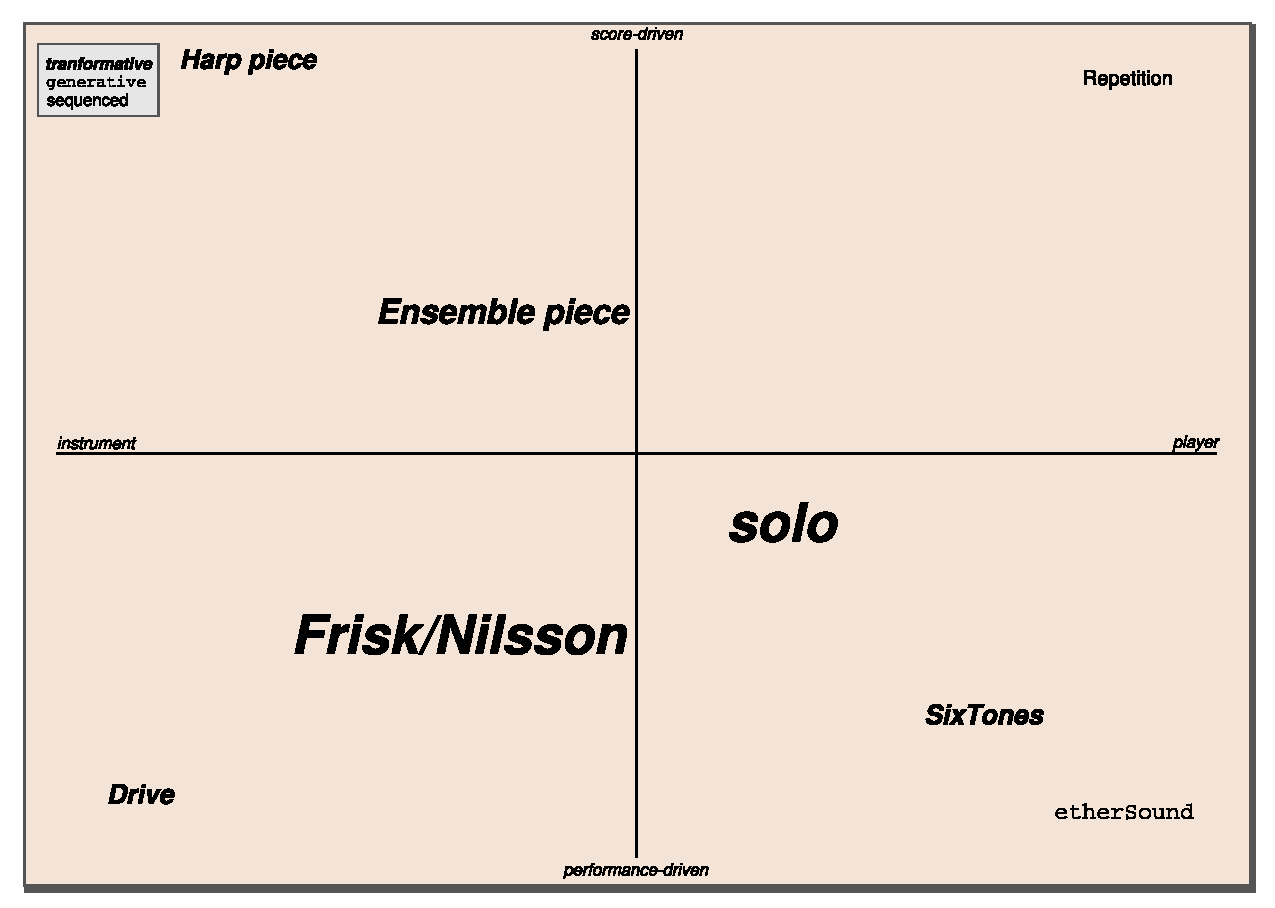
\includegraphics[width=0.97\linewidth]{img/interact-class}
%   \caption[A map of the artistic contents of the project.]{The approximate position of the artistic content in the three classification dimensions suggested by Rowe\footcite[5--8]{rowe}. The font \textit{type} is used in the graph to discriminate between the different response methods. The font \textit{size} is used to indicate the stability of the project in relation to the categories. For example, in my saxophone-computer improvisations (here depicted \emph{solo}) I use a large number of interactive techniques and programs, hence the font size is large, whereas \emph{etherSound} is fairly well categorised as a generative, performance-driven player---and is thus represented by a relatively small font size.}
% \label{fig:interact-class}
% %\end{figure}
% \end{wrapfigure}
As with any clearly delimited categorisation, the categories themselves risk producing more questions than answers (although that should not be seen only as a problem). Each kind of interactive context has its own set of requirements. A performer playing a scored piece for instrument and computer, such as \emph{Drive}, has different needs and expectations than does an improviser, and all performers do not have the same anticipations. Improvising \emph{with} a computer as a saxophonist is in every respect different from improvising \emph{on} the computer. 

%\newpage
In his book \emph{Interactive Music Systems}, composer, programmer, and researcher Robert \citeauthor{rowe} makes a classification of interactive music systems that may prove useful to help interrelations between the interactivity at play within these four sub-projects---containers of musical practice---in the context of the larger scope of the research project as a whole. I will apply these classifiers in an attempt to dismantle the concepts involved, as part of the research. For \citeauthor{rowe} the ``motivation for building such a set of classifications is not simply to attach labels to programs but to recognize similarities between them and to be able to identify the relations between new systems and their predecessors.''\footcite[6]{rowe} Although \citeauthor{rowe}, at least here, is more concerned with the actual \index{software}software in the system, categories such as those presented are also useful also in artistic work, for much the same reasons,not primarily because computer programming may be a truly artistic process, but because a methodological tool such as this (it is a classification method) allows for connections between disparate  projects to be identified in ways not possible without it.

\begin{figure}[!htb]
  \centering
  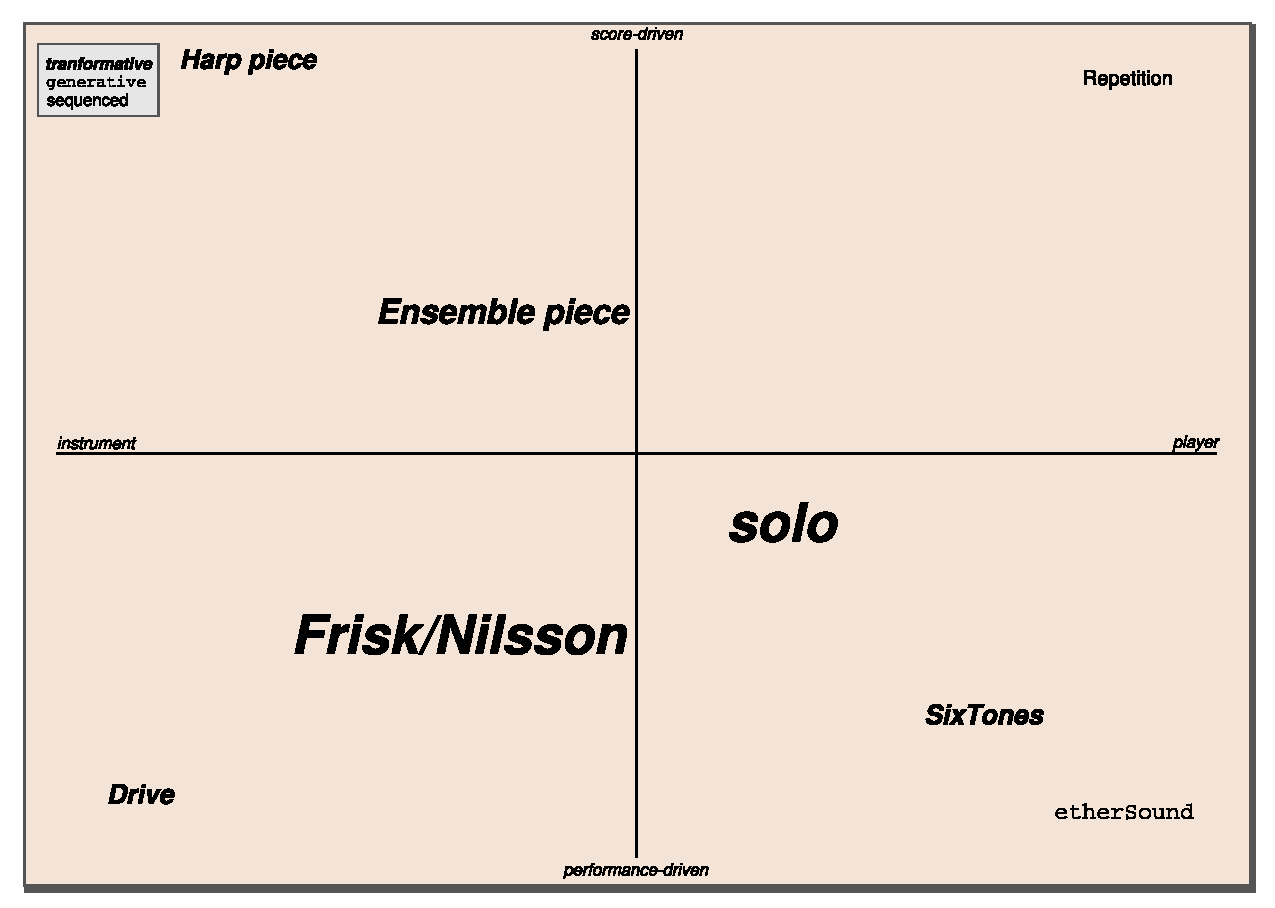
\includegraphics[width=0.9\linewidth]{img/interact-class}
  \caption[A map of the artistic contents of the project.]{The approximate position of the artistic content in the three classification dimensions suggested by Rowe\footcite[5--8]{rowe}. The font \textit{type} is used in the graph to discriminate between the different response methods. The font \textit{size} is used to indicate the stability of the project in relation to the categories. For example, in my saxophone-computer improvisations (here depicted \emph{solo}) I use a large number of interactive techniques and programs, hence the font size is large, whereas \emph{etherSound} is fairly well categorised as a generative, performance-driven player---and is thus represented by a relatively small font size.}
\label{fig:interact-class}
\end{figure}


As for the classification system, it is ``built on a combination of three dimensions, whose attributes help identify the musical motivations behind types of input interpretation, and methods of response''.\footcite[6]{rowe} That is, the way the system handles its input and how it generates its output and, according to \citeauthor{rowe}, the classifiers will provide us with a terminology which can be used to ``distinguish and draw relations between interactive programs''.\footcite[7]{rowe} 

%Though \citeauthor{rowe} uses the classifiers primarily for computer \emph{programs} I find them useful also for the point at issue.\footnote{This is likely to be because most of these projects feature at least one `program', specially designed for the purpose, even though it may only consist of a simple Max patch \parencite{max}.}

The categories in the three dimensions are:\footcite[These categories are clearly outlined in][and all the citations below are taken from p.7--8]{rowe} 

\begin{enumerate}
\item \emph{Score-driven} systems versus \emph{Performance-driven}, i.e.  systems that range from ``programs that use predetermined event collections'' (a score), to those that ``do not anticipate the realization of any particular score''.

\item \emph{Transformative}, that apply a transformation on some existing material, \emph{Generative}; that generates material from ``elementary or fragmentary'' source material (a scale or a chord), or \emph{Sequenced}, that ``use pre-recorded music fragments'', response methods.

\item \emph{Instrument} versus \emph{Player} paradigms, where the former is primarily ``concerned with constructing an extended musical instrument'', and the latter with constructing ``an artificial player'' that performs some material.
\end{enumerate}

These categories, employed in the artistic work in this project, are visualised in Figure \ref{fig:interact-class}, but it should be noted that, as is generally pointed out by Rowe,\footcite[6]{rowe} these are not fixed positions but possible starting-points. Also, as we shall see in the discussion on \emph{etherSound}, it may be very difficult to determine exactly what constitutes a `score' and, if a piece may be said to have a score which is represented in the interactive system, can it still be categorised as a \emph{performance-driven} system rather than as a \emph{score-driven} system? At any rate, the presented categories allow us to get a topological overview of the included projects' relation to different types of interactive systems in music. Further, as was briefly mentioned above, using these categories is a method adopted for reflection and presentation, not construction---I did not pre-conceive the respective projects' positions on this map. Though I did have an idea of what kind of artistic content should be included when I started this research project, none of these projects were created with the primary goal of \emph{illustrating} a method of interaction.\footnote{In a way I was surprised to see how scattered these projects were on the category map. I would have anticipated a tighter focus.} For better or worse, the only difference between my work in this artistic field within the scholarly frame of my PhD studies and the work done outside it is the added layer of reflection and the possibility to work things through more thoroughly. And, in the nature of my artistic practice---and I believe many others'---despite how rigorously a project is planned in advance, in the course of action it is bound, and should be allowed, to develop in unforeseen ways.

The one piece that most clearly lends itself to these categories is the first version of \emph{Repetition Repeats all other Repetitions}. The only possible interaction between the performer and the computer is mediated through a foot pedal---whether the pedal is down or up is the only information that the computer is `listening' to. In the other direction, as a result of the pressed pedal, there is a very complex flow of different types (classes) of information that the performer is expected to respond to: visual feedback from the computer screen on stage, physical (tactile) feedback from the pedal, auditive feedback in the sounds played back on the computer, all of which influence how the performer performs the piece. In other words, something incredibly concise and limited such as the binary distinction between pressed pedal or released pedal gives rise to a plenitude of messages of other kinds. This situation---the inconsistency between input and output---was what, at the outset of this research project as a whole, as well as at the beginning of the composition process of this particular piece, I thought of as a problem for which alternative solutions had to be invented: ``In our joint project we will attempt to avoid the kind of binary oppositions that require a clean control signal path (such as the pressing of a pedal) in the design of the interactive system''.\footcite{frisk-ost06} The foot pedal in this context is nothing more than a (non-musical) instrument to \emph{control} the computer part.

%\footnote{Compare to the discussion in Section \ref{sec:human-comp-inter} and Section \ref{sec:interaction} regarding the idea of interaction-as-control.}

In the theoretical realm the problem is the attempt to combine two radically different classes of information flow: one binary (pedal up/pedal down) and one continuous (primarily sound). The nature of the perceived response is opposite in quality to the nature of the stimulus.
%\footnote{This issue will be discussed more in the section on \emph{Interactive Music}.}
Yet, as music the piece works well,\footnote{Stefan has performed this version of the piece in Hanoi, Beijing, Malm\"{o}, Palo Alto, Seattle and Birmingham.} and I am pleased with the way the electronic sounds integrate with the guitar part. Perhaps in this piece the human-human interaction taking place in preparation for the project and Stefan's involvement in the process of composition in a way \emph{substitute} for the lack of \index{real-time}\index{time!real-time}real-time interaction? We are preparing a third version which will involve a more complex scheme of \index{real-time}\index{time!real-time}real-time interaction, not in order to prove the first version inferior (nor superior for that matter), but because it is in the nature of the piece to do several versions of it.

At the other end of the spectrum of my artistic work\footnote{\emph{Repetition...} features a (very) detailed score, and my solo work is entirely improvised; in \emph{Repetition...} I do not perform any part, but in my solo work I perform every part, and so forth.} lie my solo improvisations with computer---which on the map in \hyperref[fig:interact-class]{Figure \ref*{fig:interact-class}} are placed almost in the middle but employ a large number of different techniques---and I primarily look to achieve two things. (\textit{i}) Unity in sound (timbre) between the sounds produced acoustically and those produced electronically. This is not to say that I want the range of possible electronic sounds limited to saxophone sounds but that I look for a musical logic to the way the electronic sounds develop in relation to the saxophone sounds.\footnote{\hyperref[sec:timbremap]{See the section on \emph{timbreMap}} for further discussion on unity and sonic interaction. See also the \hyperref[sec:interraction-self]{chapter on interaction}.} (\textit{ii}) A level of interaction that is not constrained to a control interface---close to how George Lewis described a performance of \emph{Voyager} cited above (see \hyperlink{sec:target:personal-background-1}{Section \ref*{sec:personal-background}}). I too would rather have the computer surprise me than always to follow me:

\begin{squote}
In improvised music, improvisers often assert both personal narrative and difference as critical aspects of their work. For me, what Jerry Garcia called the ``anti-authoritarian'' impulse in improvisation led me to pursue the project of de-instrumentalizing the computer. If the computer is not treated as a musical instrument, but as an independent improviser, difference is partly grounded in the form of program responses that are not necessarily predictable on the basis of outside input. As we have noted earlier, Voyager's response to input has several modes, from complete communion to utter indifference. This seeming lack of uniformity is not necessarily correlated with ``lack of structure,'' as is so often expressed in the vernacular discourse of ``randomness.'' Rather, while tendencies over a long period of time exhibit consistency, moment-to-moment choices can shift unpredictably.\footcite[36]{lewis00}
\end{squote}

I think \emph{Voyager}\footcite{lewis92} is a great success as a framework for improvisation, as an interactive system, as an artistic expression that incorporates different modes of thinking about art and improvisation, and, for me, as a source of inspiration. The connection between that which is played by Lewis (and Roscoe Mitchell on the tracks that he appears on) and that which is performed by the computer is on some levels very clear yet without being obvious, and the way the musical gestures of the computer part are articulated has a distinct quality and resemblance to improvised music in a certain tradition. And this despite the fact that the computer is given no information about \emph{the sound} itself---the timbre. Only the pitch is fed to the computer.

There are obvious reasons for this choice of method of interaction in \emph{Voyager}: (\textit{i}) Pitch information may be quantified whereas timbral information can only be relative.\footnote{The definition of timbre from OED reads: ``The character or quality of a musical or vocal sound (distinct from its pitch and intensity) depending upon the particular voice or instrument producing it, and \emph{distinguishing it from sounds proceeding} from other sources''. The Oxford English Dictionary.  2nd ed. 1989. OED Online. Oxford University Press. (visited 14/11/2007). \url{http://dictionary.oed.com/cgi/entry/50252865} (my italics). It may be noted that, according to OED, two different sounds emanating from the same source---say a key click and a regularly played note on a saxophone---are not of different timbre. According to my understanding of timbre (and the English language) the last three words should be changed to ``from the same or other sources''.} Therefore pitch lends itself much more naturally to use as input in an algorithmic system of transformations.\footcite[Compare with \index{electro-acoustic music}electro-acoustic music composer and improviser Trevor Wishart's reasoning in][chap. 2]{wis96} (\textit{ii}) At the time \emph{Voyager} was created the technology for achieving and collecting information about timbre in \index{real-time}\index{time!real-time}real-time was very limited. (\textit{iii}) Even if information about timbre was to be extracted from the signal in \index{real-time}\index{time!real-time}real-time, the available \index{real-time}\index{time!real-time}real-time synthesis techniques were somewhat limited (and costly) at the time. (\textit{iv}) It may be a perfectly viable artistic choice to let the computer part have this quality of disruption, a quality of sound distinct from the acoustic sounds.

Musicologist Ingrid \citeauthor{monson96}, in her book on \index{interaction!musical}musical interaction in the jazz tradition, refers to the Charles Mingus-Eric Dolphy duet on the beautiful tune \emph{What Love}\footcite{mingus60} in which, according to \citeauthor{monson96}, it sounds ``as though they were having a very intense verbal argument''. Much later in the book, she returns to this recording and
the nature of the Mingus/Dolphy `argument':
\begin{squote} 
If I were to transcribe the notes and play them on the piano, they wouldn't sound very much like the conversation on the recording, for it is the relatively non-notable timbral and dynamic inflections produced by the players that are the principal means of signifying the iconicity.\footcite[208]{monson96}
\end{squote}
\hypertarget{sec:target:music-pract-inter-1}{When I listen to} \emph{Voyager}, I hear the playing of Lewis and Mitchell in a similar way: the particularity of that which is `said' is encoded in the \emph{sound} rather than the \emph{pitch}. This is, however, not how I perceive the voices of the computer part whose timbres are remarkably dull and static in comparison. To me, there is a perceptual breach between the electronic sounds and the acoustic sounds. 

\begin{wrapfigure}{r}{0.3\linewidth}
  \begin{minipage}[h]{\linewidth}
    \begin{flushright}
      \musicannot{Improvisations\\
        \emph{ for saxophone and computer}\\
        Performed in 2005}
    \end{flushright}
  \end{minipage}
\end{wrapfigure}

%%% Local Variables: 
%%% mode: latex
%%% TeX-master: "../ImprovisationComputersInteraction"
%%% End: 

My research project is in part the attempt to address this breach in my own work and this is what I referred to above as the ambition to look for unity between acoustic and electronic sounds. In the improvisation entitled \emph{Insanity} I do it by placing a restriction on myself as to what sounds I allow myself to produce (percussive sounds only), and in the accompanying program I use a technique for analysis/re-synthesis that I know works well for that class of timbres. In the improvisation \emph{A Call for Response} I use an analysis/re-synthesis technique that works well for multiphonics and focus my improvisation on a series of multiphonics.  In both of these examples the connection between the acoustic timbres and the electronic sounds is pre-conceived. They are encoded and static and should I wish for an improvisation suddenly to follow a different path, the pre-composed connection would fail. Though such failure does not necessarily imply that the music as such will fail, I nevertheless see it as a problem. The \emph{timbreMap} program is a general attempt to address this issue and allow for more dynamic coupling between the performed acoustic timbres and the resulting electronic timbres.

In the next chapter I will discuss the interactive sound installation \emph{etherSound} wich played an important role in the way my view on interaction was expanded. Its background is presented as well as the design of the system and a reflection on interactive sound installations and public participation is provided. As \emph{etherSound} was one of the earlier sub-projects I started, the following chapter was written over the course of several years but has been continually reworked. 
\newpage
\thispagestyle{empty}
% Although, in part, this ambition is dependent on extracting and % communicating the `right' information to the computer, it may equally % well be necessary to approach the issue by other means. 

% What \citeauthor{monson96} is saying is that it is in the % microvariations that the communication is taking place
% When Monson brings up `iconicity' she also reveals another layer of % disruption in the pitch-tembre relation. Iconic communication, much % like the unconscious and most art is encoded according to primary % process. Pitch on the other hand, and the logic of the tempered % system, is organized according to secondary process.

%%% Local Variables: 
%%% mode: latex
%%% TeX-master: "../ImprovisationComputersInteraction.tex"
%%% End: 


%%%%%%%%%%%%%%%%%%%%%%%%%%%%%%%%%%%%%%%%%%%%%%%%%%%%%%%%%%%%%%%%%%%%%%%%%%%%%%%%
%% Interaction
%%%%%%%%%%%%%%%%%%%%%%%%%%%%%%%%%%%%%%%%%%%%%%%%%%%%%%%%%%%%%%%%%%%%%%%%%%%%%%%%
\chapter[\emph{etherSound}]{\emph{etherSound}}
\label{sec:ethersound}
\begin{wrapfigure}{r}{0.4\linewidth}
  \begin{minipage}[h]{\linewidth}
    \begin{flushright}
      \musicannot{etherSound\\
        \emph{for improvising musicians, audience and mobile phones.}\\
        Composed \& premiered in 2003\\
        Commissioned by Miya Yoshida}
    \end{flushright}
  \end{minipage}
\end{wrapfigure}

%%% Local Variables: 
%%% mode: latex
%%% TeX-master: "../ImprovisationComputersInteraction"
%%% End: 

\emph{etherSound} was commissioned by curator Miya Yoshida for her project \emph{The Invisible Landscapes} and was realised for the first time in August 2003 at \emph{Malm\"{o} Art Museum} in the city of Malm\"{o}, Sweden. The curatorial concept for \emph{The Invisible Landscapes}  project was the use of cellular phones in the context of experiencing and creating artistic expressions. The principal idea behind \emph{etherSound} was an attempt at developing an instrument that can be played by anybody who knows about how to send an SMS (Short Messages Service) from their cellular phone. The focus of my artistic research project, of which \emph{etherSound} is a part, is the interaction between computers and musicians as well as non-musicians. \emph{etherSound} is an investigation of some of the aspects of interaction between the listener, the sounds created and, in the performance version of it, the musicians playing, and also of the formal and temporal distribution of the music that this interaction results in. 

Although interaction is an important aspect of any musical performance---as well as a part of any music listening activity, to music performed live or otherwise---opening up a musical work to anyone except trained musicians is not a trivial task; careful attention has to be paid to the purpose for doing so and to the intentions of the work. It is relevant to pose the question whether it is possible to reach a satisfactory result with almost no limitations on participation. 
%%%Is this satisfactory result technological or aesthetical? And how would you evaluate the result? %%%
Before these questions can be addressed, however, we need to delineate the reasons for wanting to allow public participation. 

Public participation has been explored in the visual arts for many years, for artistic as well as political reasons: ``All in all, the creative act is not performed by the artist alone; the spectator brings the work in contact with the external world by deciphering and interpreting its inner qualification and thus adds his contribution to the creative act'' \footcite{duchamps57}. The French curator and art critic Nicolas \citeauthor{bourriaud} speaks of ``\textit{relational} art'' (italics by the author) described as ``an art taking as its theoretical horizon the realm of human interactions and its social context, rather than the assertion of an independent and private symbolic space.''\footcite[13]{bourriaud}
If we look at it from a performing arts perspective, the audience visiting a performance can be said to participate in it - if only in a limited sense. As \citeauthor{adorno} points out, however, in the spheres of distribution and consumption of music, the musical work is objectified---reduced to a mere social commodity which severely limits the freedom of choice and influence of the listener\footcite[p. 211]{adorno}. In combination with the near monopoly of the multinational corporations of production and distribution of music, though the producers will always plead the public taste (``the manipulator's reference to the manipulated is empirically undeniable''\footcite[p. 212, my translation.]{adorno}), it is difficult to claim \index{audience participation}audience participation in a general sense. Furthermore, Western art music is to a considerable extent looked upon as a hierarchical process; a process that begins in the mind of the composer and ends at the level of the listener or even before that, at the level of interpretation. It is fair to assume that bringing in an uncontrollable agglomeration of participants influencing the distribution of musical events will disturb this order. 

In their article on the multi-participant environment \emph{The   Interactive Dance Club}, multi-media artists Ryan Ulyate and David Bianciardi define one of the design goals as wanting to ``deliver the euphoria of the artistic experience to `unskilled' participants''.\footcite[41]{ulyate} Rather than merely sharing the result with an audience, they attempt to unfold the creative process leading to the result and invite the audience to take part in this process: ``Instead of dancing to prerecorded music and images, members of the audience become participants. Within interactive zones located throughout the club, participants influence music, lighting, and projected imagery'' (p. 40). The activities normally engaged at a dance club are not only performed as a result of the music played, but also used to influence the music. Similar ideas are put forward by Todd Machover concerning his large scale, interactive work \emph{The Brain Opera}: ``\emph{The Brain Opera} is an attempt to bring expression and creativity of everyone, in public or at home, by combining an exceptionally large number of interactive modes into a single, coherent experience''.\footcite[Machover, 1996, as quoted in][p. 360]{rowe01} These ambitions point to one of the big challenges of building interactive environments: how to design musical interfaces that have a ``low entry fee, with no ceiling on virtuosity''.\footcites{wessel}{jorda02}[See also][]{rowe}{auracle} With the recent technological advances there are innumerable tools that can be used for collaborative efforts,\footcite{barbosa02} affordable devices that may easily be used as interfaces to computer mediated art works (game controllers, mobile telephones, GPS navigators, web-cams, etc.). Not only has this the potential of changing our perception of the arts, it can also help us understand this new technology and the impact it has on our lives.
%%%A more general question after reading this paragraph: Is there a political (ethical, social) agenda to audience participation? %%%

A project for which public participation is important must somehow deal with the aspect of access, and according to Pierre \footcite{bourdieu} there is an intimate association between social class, level of education and cultural interests that affects cultural consumption:
\begin{squote}
The experiences which the culturally most deprived may have of works of legitimate culture [\ldots] is only one form of a more fundamental and more ordinary experience, that of the division between practical, partial, tacit \textit{know-how} and theoretical, systematic, explicit \textit{knowledge} [\ldots], between science and techniques, theory and practice, `conception' and `execution', the `intellectual' or the `creator' (who gives his own name to an `original', `personal' work and so claims ownership) and the `manual' worker (the mere servant of an intention greater than himself, an executant dispossessed of the idea of his own practice) (p. 387, italics by the author). 
\end{squote}
Bourdieu is telling us that because ``ordinary workers'' are ``[l]acking the internalized cultural capital'' they lack access to ``legitimate culture''. Instead they are referred to `` `mass market' cultural products---music whose simple repetitive structures invite a passive, absent participation'' (p. 386). Perhaps \emph{active} and \emph{present} participation can counteract the effects of lack of cultural capital? Bourdieu couples the ordinary class border divisions with the experience the working class may have of legitimate culture. I would like to suggest, however, that the association between social and cultural class and consumer electronic devices like the mobile phone, and the behaviours associated with its use, are of a different nature from the association between class and cultural consumption. If entree to the art-work is mediated through an interface (in this case the mobile phone) for which access is not governed by the same rules as the conception of contemporary art this may help level the playing field. 
%%%For sure you’re able to make an audience participate but how satisfactory is that (for them, as an aesthetic result, as a political statement)? %%%
This is a motion that works externally, from the outside in, distorting the experience of division (owing to lack of cultural capital) between the un-initiated spectator and the work. But, as we will see, there is another equally important factor at play that works from within the work. Distributing the role of the `` `creator' (who gives his own name to an `original', `personal' work and so claims ownership)'' (p. 386) to several agents---anyone interacting with the work is in fact part of the creation of it---means the listener/performer and performer/composer dichotomies are blurred and thereby another opening is created that helps provide access to the art-work. 

Roy \citeauthor{Ascott}, in addressing the issue of `content' in art involving computers and telecommunications writes:
\begin{squote}   In telematic art, meaning is not something created by the artist,   distributed through the network, and \emph{received} by the   observer. Meaning is the product of interaction between the observer   and the system, the content of which is in a state of flux, of   endless change and transformation. (p. 241, italics by the author).
\end{squote}
As opposed to the classical notion of the educated `creator' who claims `authorship' (to use the language of Bourdieu), in collaborative, telematic art-works not only is meaning a consequence of interaction, the concept of `the work' is also greatly affected. The \index{ontology}ontology of the musical work or the `work concept' in music is a complex field which is dealt with in more detail in the essays entitled \emph{Negotiating the Musical Work}. \footcite{frisk-ost06,frisk-ost06-2} \citeauthor{Ascott}, however, is mainly concerned with the visual arts in which the question of the work concept is of a different order, and makes an interesting point when substituting \textit{interface} for \textit{art object}:
\begin{squote}
The culturally dominant objet d'art as the sole focus (the uncommon   carrier of uncommon content) is replaced by the interface. Instead   of the artwork as a window onto a composed, resolved, and ordered   reality, we have at the interface a doorway to undecidability, a   dataspace of semantic and material potentiality. The focus of the   aesthetic shifts from the observed object to participating subject,   from the analysis of observed systems to the (second-order)   cybernetics of observing systems: the canon of the immaterial and   participatory. Thus, at the interface to telematic systems, content   is created rather than received.
\footcite[242]{Ascott}
\end{squote} 
Transposed to the field of music then, the \emph{the work} is replaced by the \emph{interface}. Applied to \emph{etherSound}, the mobile phone as interface becomes the work and the number of participants and their contributions become the \index{ontology}ontology of whatever work we can speak of. The interface acts as the (only) way to navigate the space created by music.

Though less centred on public participation and more on improvisation, Guy E. \citeauthor{Garnett}, composer and computer scientist, touches on some of the same issues in his article on interactive computer music aesthetics considering the potential for change in ``unfixed works'' such as ``human improvisation with computer partner'': 
\begin{squote}   
Since the human performance is a variable one, by its nature, that  variability can become the focus of aesthetic issues, even simple  ontological issues. Because the performance changes from time to  time and from performer to performer, the notion of `the work'  becomes more and more clouded. The work, even from an objective  rather than an immanent point of view, becomes something open-ended.  Each performance becomes an `interpretation' of the possibilities  inherent in whatever was `composed.' However, each of these concepts  is highly problematic. This `interpretation' can have significant  consequences for the meaning - and therefore value - of a work in a  cultural context. Since the work is not fixed, it is open to new  interpretations, and therefore the possibility at least exists for  the growth of the work over time or across cultural boundaries. The  work can thus maintain a longer life and have a broader impact  culturally, because it is able to change to meet changing aesthetic  values. (p. 27) 
\end{squote} 
As is hinted at by Garnett himself, the idea of interpretation becomes troublesome in the context of improvised music and I will discuss the issue of the work identity in more detail in \hyperref[sec:ident-emph]{Section \ref*{sec:ident-emph}}. As far as \emph{etherSound} is concerned, it cannot be performed \emph{without} public participation. As music it holds no significant value unless there is a group of people interacting with it---its value is embedded in the interaction and in this way it differs from a written score or a pre-structured improvisation.\footnote{A written score of music may be said to have musical value in itself. Although I personally argue against it, it   may even be said to constitute the work. My argument here, shared by   \citeauthor{Ascott} and \citeauthor{Garnett}, is that an interactive   attitude towards music-making changes the conditions for how the   identity of the work may be established.}  Further, the understanding of it is not necessarily related to the contextualisation of the sounds produced within the history of (interactive) electronic music but may instead be regarded as one factor in the relation between the expectations of the subject interacting and the music produced.  Following these lines of thought, it may be concluded that the need for a thorough ontological understanding of the history of art or electronic music is not a prerequisite for understanding a collaborative, interactive work of music---anyone willing to interact and interested in making a contribution is equally well prepared to produce and interpret the `meaning' of \emph{etherSound} . This limits the advantage of the educated listener---``the dominating class'' \footcite{bourdieu}---and makes room for new interpretations of the term `understanding' in the arts. \footnote{This issue is also discussed in \cite{frisk05}.}. 

%%% Local Variables: 
%%% mode: latex
%%% TeX-master: "../ImprovisationComputersInteraction"
%%% End: 

\section{The Design} 
\emph{etherSound} is an attempt to open a musical work to the un-initiated listener, including him or her in the creation of the music, and provide for a notion of `equality of participation': all contributions are equally valuable. Accessibility without prior knowledge of music or musical training is an end in itself in this project. It should be noted that this obviously presupposes that the participant knows how to send an SMS and that the system makes it difficult for those who are not familiar with this technology.\footnote{At the time this project was initiated, however, there was great commercial interest in increasing the use of SMS and in Sweden there has been a concerted effort on the part of the GSM service providers to teach their customers how to use it.} It should also be made clear that using SMS text messages for interaction, as implemented here, does not allow for direct dynamic control. Every message generates one `message-composition' and all control data are derived from the content of the message.

\begin{figure}[hbp]
\begin{center}
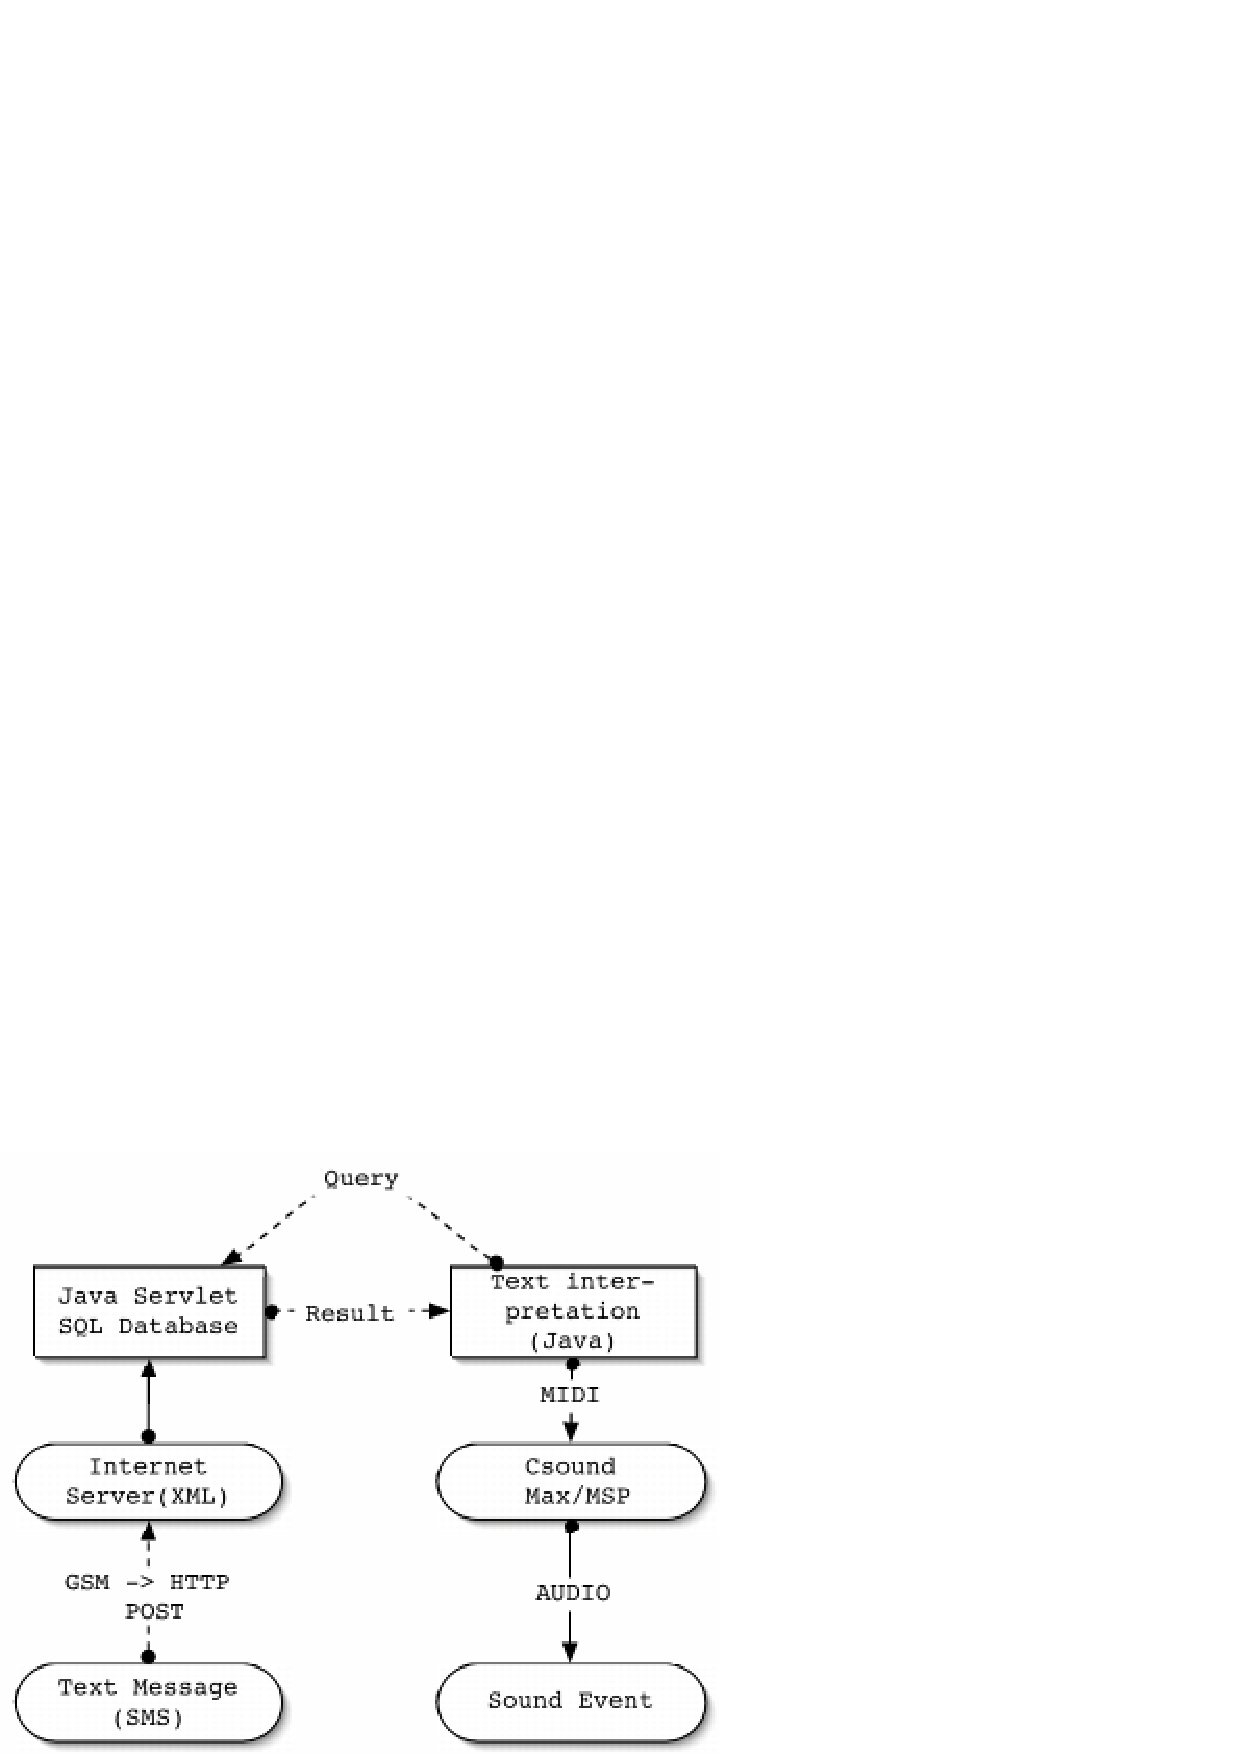
\includegraphics[width=0.45\textwidth]{img/ethsnd/Figure1}
\caption{Communication in the first version.} \label{model1}
\end{center}
\end{figure}

\subsection{Communication---first model}
\label{sec:comm-first}
In the first version, realised in August 2003,\footnote{See the audio   and video recording \emph{etherSound}/\emph{etherSound 2003}.} the communication between the participant and the system was accomplished according to \hyperref[model1]{Figure \ref*{model1}}. An SMS sent to a specified number was transformed to an XML file (eXtensible Markup Language, see \url{http://en.wikipedia.org/wiki/XML}) and transferred to a URL by an HTTP POST request. This part was handled through an external service. At the called URL, a JSP (Java Server Pages)  directed the POST data to a Java Bean\footcite{j2ee} that handled the parsing of the data and the connection to a MySQL database in which it created a new entry with the relevant fields. 

It was owing to security reasons at the museum where this version was realised that the HTTP request could not be handled locally. Instead, the local computer queried the server database for new entries on regular intervals.  After some testing, sending a SQL query once every second seemed like a reasonable time interval. Shorter time intervals did not accomplish a perceivably quicker response time and, since the synthesis program was running on the same machine, I did not want to use more processing and network activity than was necessary for this task. After the text message had been processed, control signals were sent by \useGlosentry{glos:MIDI}{MIDI} to the synthesis engine. 

As is obvious from the recordings of the two versions, the sounds produced by the computer in this first version are very different from those in the second recording.

\begin{figure}[hbp]
  \begin{center}
    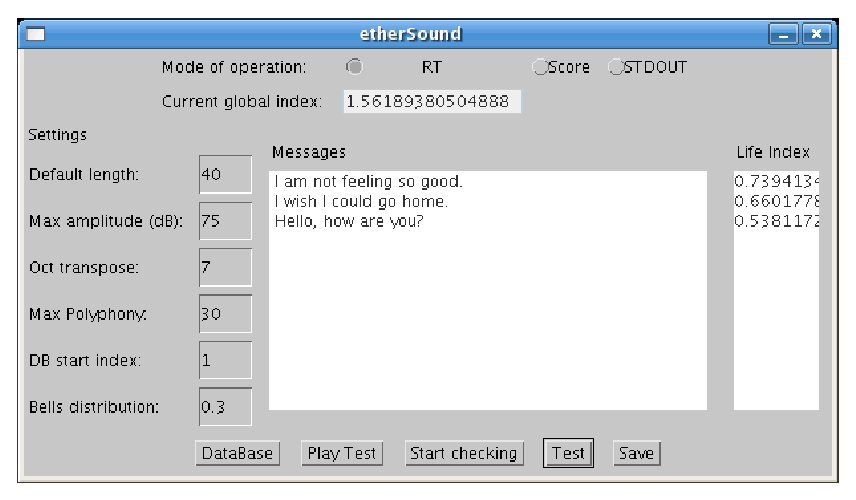
\includegraphics[width=0.9\textwidth]{img/ethsnd/MainGUI}
  \caption{Main GUI window for the \emph{etherSound} program.}
  \label{fig:main_gui}
\end{center}
\end{figure}

\subsection{Communication---current model}
Although the first version worked well and was fairly stable, it was a solution that required an external SMS processing service, and a local, reliable network connection. In order to make the piece more `portable' and independent, the message-receiving part was rebuilt. Using the gnokii API\footcite{gnokii} it is relatively easy and reliable to connect a GSM phone to a computer and gain access to the storage and status of the phone which enable reception of the SMS messages locally. To retain the possibility of reviewing the activities of transmission, the messages are, just as in the first model, written to a database. In other words, the client-server model is retained but on one and the same machine. Furthermore, the MIDI connection between the control application and the synthesis engine was replaced with \index{Open Sound Control}\index{OSC}Open Sound Control (\useGlosentry{glos:OSC}{OSC})\footcite{osc, osc_web} for speed, reliability and flexibility, using the library JavaOSC.\footnote{See \url{http://www.mat.ucsb.edu/~c.ramakr/illposed/javaosc.html}.}

\begin{figure}[hbp]
  \centering
  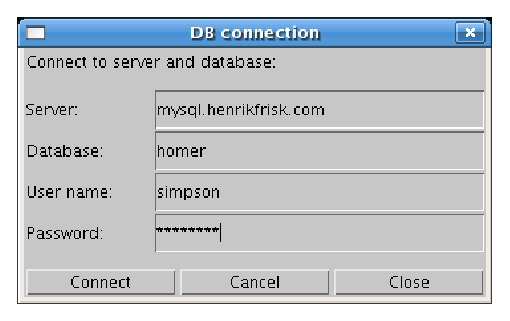
\includegraphics[width=0.5\textwidth]{img/ethsnd/DB_connection_window}
  \caption{Panel for connecting to the database.}
  \label{fig:DBpane}
\end{figure}

\subsection{The text analysis}
The program handling the text processing and the mapping of text to control signals for the sound synthesis is written in Java \footcite{j2se} and features a simple but useful Graphical User Interface  \index{GUI (Graphical User Interface)}GUI) for control and feedback about the status of the system (see Figure \ref{fig:main_gui} and Figure \ref{fig:DBpane}).  

% It is in the mapping % between the text and the synthesis and sequencing of the sound events % that the musical potential of the system is constructed.  From the information extracted from the message control signals are generated which then influence (ordered from general to specific): 
\begin{itemize}
\item{The length of the whole event}
\item{The rhythm and articulation of the individual sound events}
\item{The pitch and character of individual sound events}
\end{itemize}
There are two parameters controlling the timing of events; a local `life' index shaping the rhythms and the length of the current message and a global index that influences the current and subsequent `message-compositions'. The global index is a function of the current and previous messages local indexes. The local index is a result of a simple semantic analysis of the message. It indicates the message's relative structural complexity and allows the algorithm to discriminate between messages with a set of random letters and messages with real words and real sentences. The participant should be rewarded for the effort of writing a message with substance, where `substance' is defined here as a message with a credible average word length and a reasonable distribution of vowels within these words. In the analysis substitutions are made to allow for (i.e. not punish) idiomatic SMS writing such as `R u here?' or `C u 2 nite'. These examples are expanded into their `correct' equivalent. Standard abbreviations are also expanded. 

The local index is calculated by looking at the average length of words and the average number of syllables per word and comparing these with constants: 

\begin{equation}\label{index}
i_1=\frac{1}{(w(\frac{c}{w_c})-w_l)^{1/2}+1} \qquad i_2=\frac{1}{(w(\frac{s}{w_c})-s_l)^{1/2}+1}
\end{equation}

where $c$ and $s$ are the total number of characters and syllables, $w_c$ is the number of words in the current message and $w_l$ and $s_l$ are constants defining the `optimal' mean number of words/syllables. $w$ is a weight defined by 
\begin{equation}
w=\frac{1}{w_c-s_c+0.5}
\end{equation}

where $s_c$ is the total number of words that contain vowels. Through $w$, the index is decreased if the message contains words without vowels. The mean value of $i_1$ and $i_2$ is then multiplied by the arcus tangens of the number of words in relation to a third constant parameter, $o_w$, delimiting the optimal number of words per message\footnote{Since an SMS is limited to 160 characters these   constants are set according to what kind of message content should   be rewarded.} according to \eqref{life}.

\begin{equation} \label{life}
lifeIndex = \frac{i_1+i_2}{2}{\arctan (\frac{w_c}{o_w})}
\end{equation}

If we set $w_l$ to 4.5, $s_l$ to 2.0 and $o_w$ to 10 the result in four different messages can be seen in Table \ref{result}; the method distinguishes fairly well between nonsense and real words at a low computational cost. Similar or better results could conceivably be achieved in a number of different ways but this method appears to work well for the purpose.

  \begin{table}[!tbp]
    \begin{center}
      \begin{tabular}{l|r}
        \hline
        \textbf{Message} & \textbf{Life index} \\
        \hline
        \small{hello} & 0.18882 \\
        \hline
        \small{\textit{Hello, my name is Henrik}} & \textit{0.81032} \\
        \hline
        \small{hjdks la s duyfke jhsldf hasdfiw uehr jkdsl} & 0.14448 \\
        \hline
        \small{\textit{From fairest creatures we desire increase,}} & \textit{1.44618} \\
        \small{\textit{\ \ \ \ That thereby beautys rose might never}} & \\
        \hline
      \end{tabular}
      \caption{Life index for four different messages.} \label{result}
    \end{center}
  \end{table}

  The total length of the music derived from the message is calculated   by multiplying a constant preset time with the local index. Any new   message received adds its local index to the instantaneous global index which decreases exponentially at a set rate.\footnote{The rate is context-dependent. In a performance with improvisation it would be shorter than in an installation.} If a message causes the global index to reach maximum, it stops the playback of the current   message and begins playing back a pre-composed pattern, sonically   different from the output of a typical message, for about 30 seconds   before resuming ordinary mode and starts playing back the message   that caused the break. This feature is added to reward collaborative   efforts. The global index mainly controls the density and the   overall volume of the output, but also the distribution of random   and stochastic processes in the synthesis. 

\subsection{The synthesis}

The synthesis engine is written as a \useGlosentry{glos:csound}{Csound} orchestra.\footcite{csound} \footnote{For more information on Csound see also \url{http://www.csounds.com/}} In the first versions of \emph{etherSound} Csound was running inside a \index{Max/MSP}Max/MSP (\url{http://www.cycling74.com/products/maxmsp.html}) patch through the use of the \texttt{csound$\sim$} object (see \url{http://www.csounds.com/matt/}). The Csound score for the message to be played back was sent to \index{Max/MSP}Max/MSP using \useGlosentry{glos:OSC}{OSC}. \useGlosentry{glos:Max}{Max/MSP} was responsible for timing the note events and preparing valid information for the \texttt{csound$\sim$} object and the orchestra file associated with it. Owing to processing power limitations only one message could be played back simultaneously; if a message was received before the previously received message had finished playing back, the new message would interrupt the current message (this can be clearly heard in the recording of the performance from 2003). In the latest version of the \emph{etherSound} \index{software}software, instead of sending the Csound score events being sent over OSC, they were sequenced and written to the standard output and sent to Csound through a UNIX pipe. Also, rather than the number of voices being limited by new messages crudely cutting off currently playing messages, the number of simultaneous voices available is now set in the \emph{etherSound} \index{GUI (Graphical User Interface)}GUI (see Figure \ref{fig:main_gui}) and may be changed dynamically. The following discussion relates to the current version of \emph{etherSound}. 

\begin{figure}[!hbp]
  \centering
  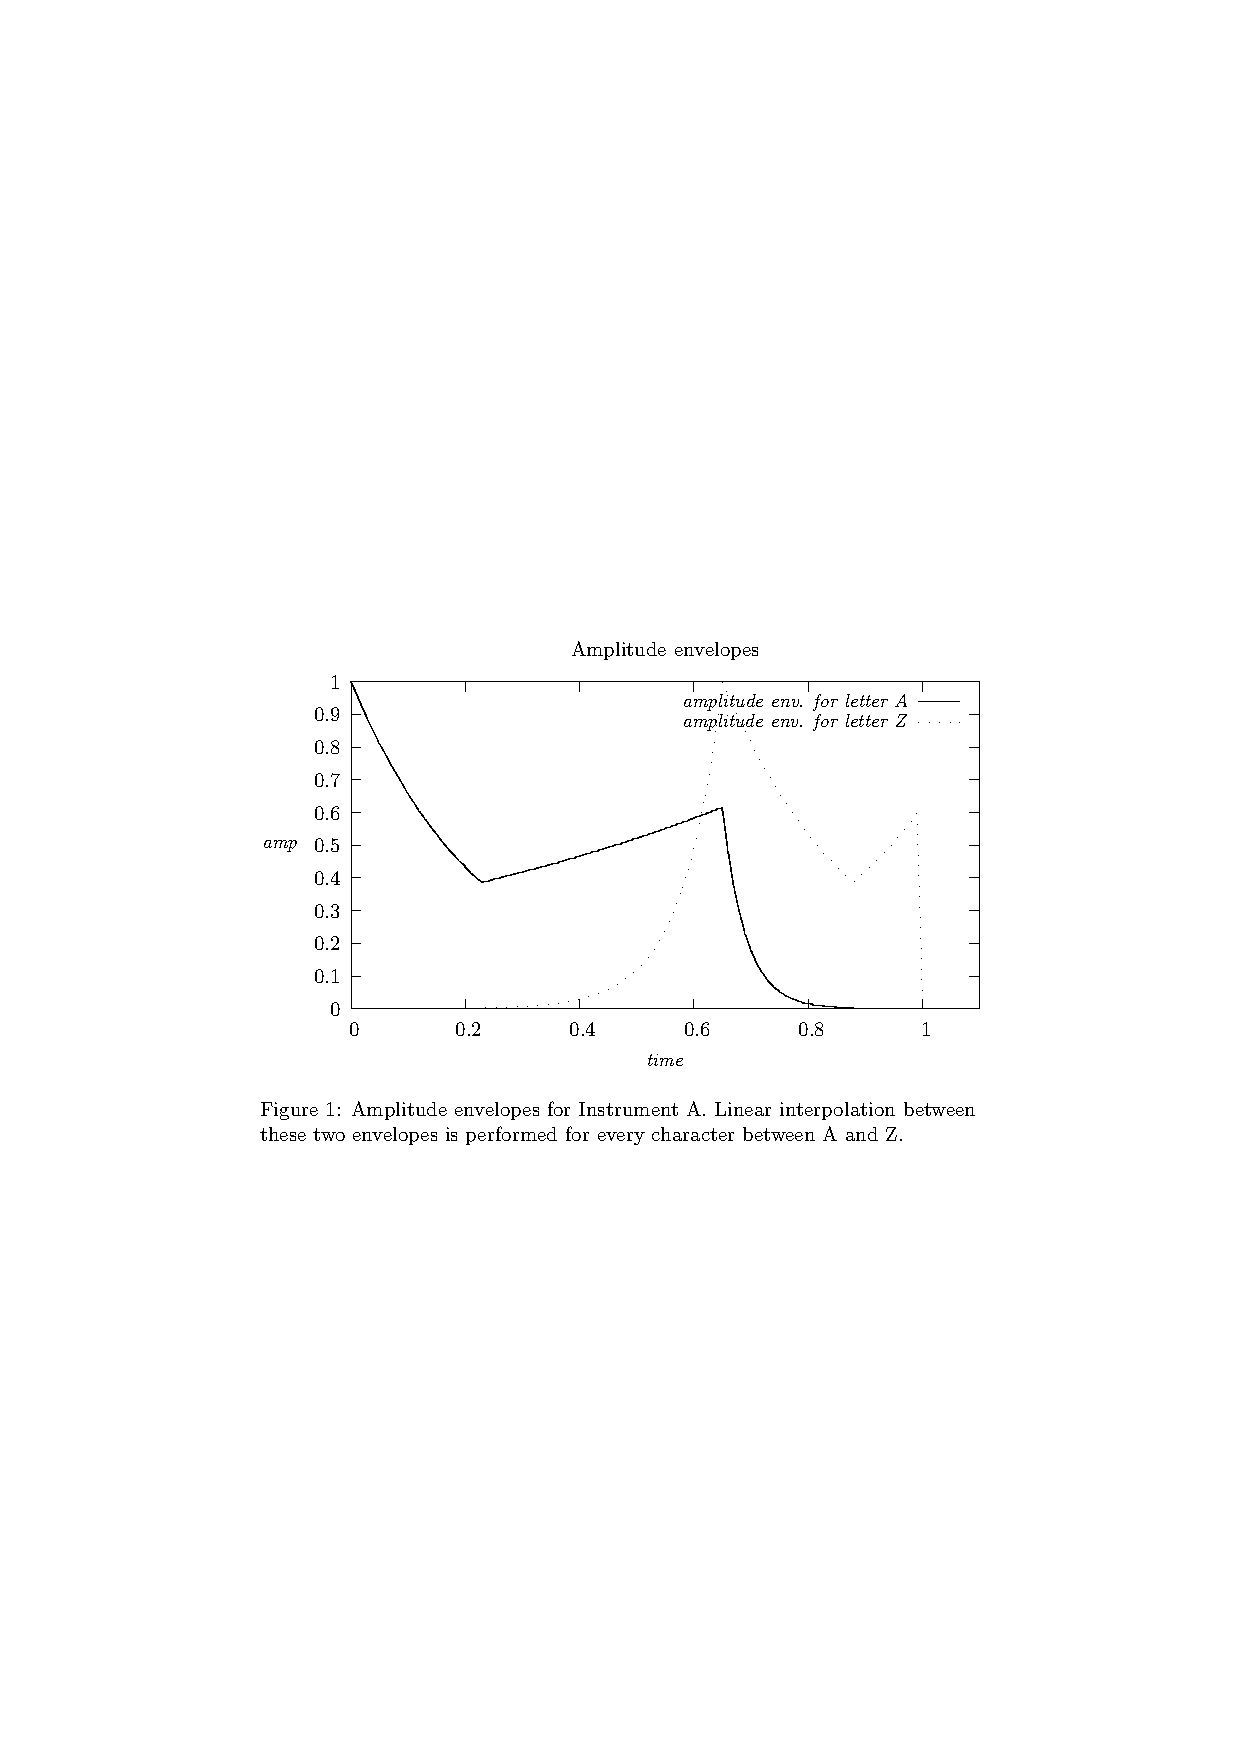
\includegraphics[trim=40mm 120mm 0mm 80mm, clip, height=50mm]{img/ethsnd/envelope}
  \caption[Amplitude envelopes for \emph{etherSound}: Instrument A.]{Amplitude envelopes for Instrument A. Linear interpolation
    between these two envelopes is performed for every character
    between A and Z.}
  \label{fig:envelope}
\end{figure}

All sounds heard in \emph{etherSound} are generated with FOF (Fonction d'Onde Formantique) synthesis, as this technique is implemented in Csound,\footcite{fof,fof2}, using both samples and simple sine waves as sound sources. There are two distinct timbres played by two different instruments in each message-composition: (A) granulated samples of a male reading a text in English\footnote{An excerpt from the recording of one of John Cage's lectures at Harvard College 1989.} and (B) a bell-like sound whose formants are matched to and interpolated between the series of vowels in the text.  

\subsubsection{Instrument A} Every word of the message is considered as one phrase or \emph{bar} of music in the resulting message composition. The number of beats per bar is approximately equal to the number of syllables in the word, where a syllable is defined as a vowel or group of consecutive vowels or a punctuation mark. The rhythmic subdivision of each bar is equal to the number of characters, including punctuation and white space, in each syllable. Thus, a monosyllabic word such as `my' followed by a white space results in a phrase consisting of one bar of one beat and two notes and one pause, i.e. three (eight-note) triplets of which the last is silent (see Table \ref{time}). If a word ends with a full stop, a comma, an exclamation mark or a question mark, more emphasis is put on the end of the bar containing the punctuation mark and the last note of the resulting phrase will be elongated. A note close to a vowel is more likely to be accented than a note further away from a vowel. 

The amplitude envelope curve of each note is related to the letter to which the note corresponds. Envelopes are mapped linearly to characters; the letter `A' has a short attack and a long decay and the letter `Z' has a long attack and a short decay (see Figure \ref{fig:envelope}). The amount of overlapping between notes, i.e. the lengths of the notes, is influenced by the current life index \emph{and} the global index where higher values will result in longer notes and thus in smoother transitions between timbres. The notes of Instrument A do not have a perceivable pitch. Twenty-eight short sample buffers (typically 32.768 samples or approximately 0.7 seconds), one for each letter, are dynamically mapped one to one to the characters in each message. The FOF synthesis is used to granulate these samples, creating an erratic, non-tonal texture but still, in most cases, reminiscent of speech. 
\begin{figure}[!htb]
  \begin{center}
    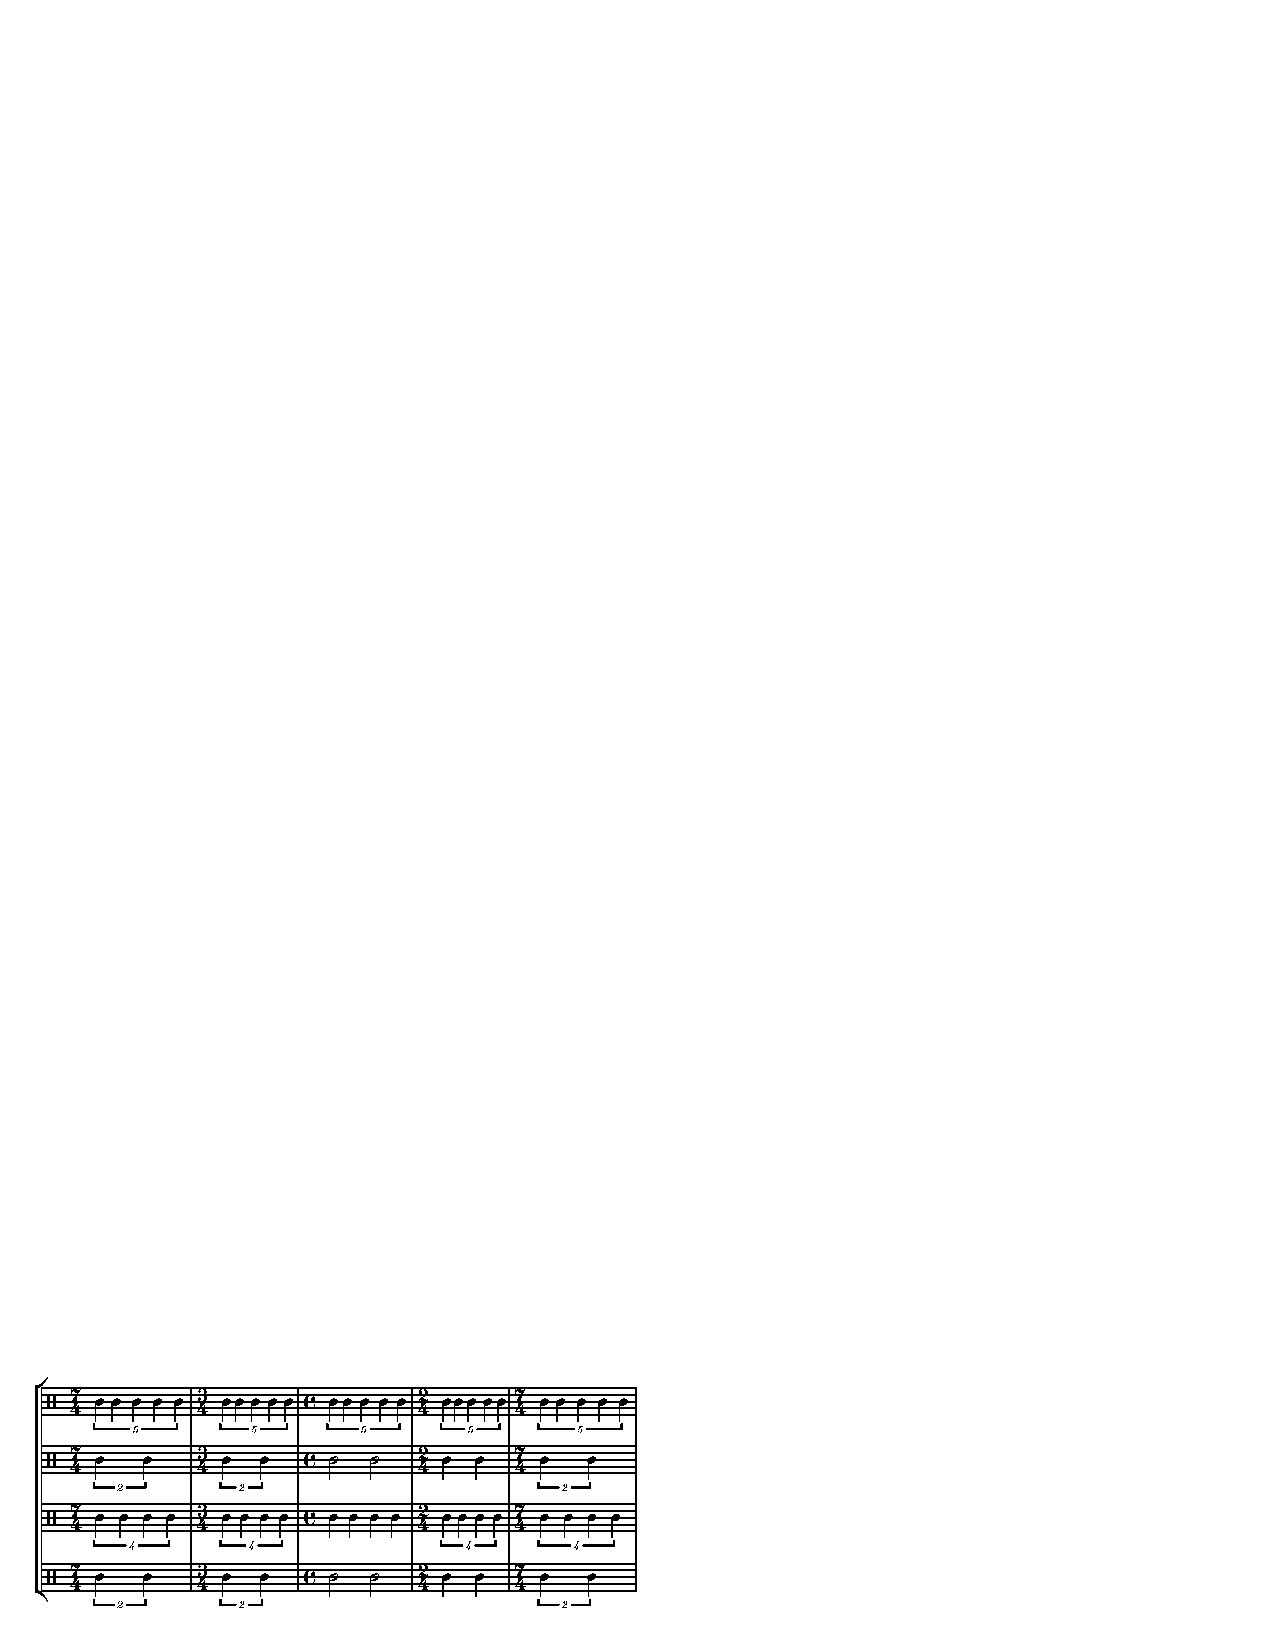
\includegraphics[width=0.75\textwidth]{img/ethsnd/harm}
    \caption[Rhythmic distribution of notes in \emph{etherSound}: Instrument B]{Rhythmic distribution of notes in Instrument B as a
      result of the message ``\emph{Hello, my name is
        Henrik.}''} \label{time2}
  \end{center}
\end{figure}

\subsubsection{Instrument B}
The phrasing of the notes of the second instrument is somewhat more complex than that of Instrument A. This instrument has, at the most,\footnote{As already stated, the maximum number of voices is set based on what the   processing power of the system is.} as many voices as there are words in the message. An example of the rhythmic mapping of notes is shown in Figure \ref{time2}, the origin of which is the message in Table \ref{time}, with the polyphony limited to four voices. For this instrument the number of beats per bar (i.e. per word) is equal to the number of letters per word, including trailing punctuation marks and white space. If there are fewer words than the maximum polyphony, the number of voices is equal to the number of words; the first voice corresponds to the first word, the second voice to the second word and so on. For every bar, each voice has as many potential excitations as there are letters in the corresponding word. After the initial excitation, which will always be played, the likelihood that a given note will be played is related to the life index \emph{and} the global index: if the normalised sum of the local index and the global index is 0.5, half of the excitations will be performed. The amplitude envelope curve for the notes played by this instrument is either of a bell-like character or its inversion, and notes close to the beginning of a bar have a greater likelihood of being emphasised. 

\begin{figure}[!htb]
\begin{center}
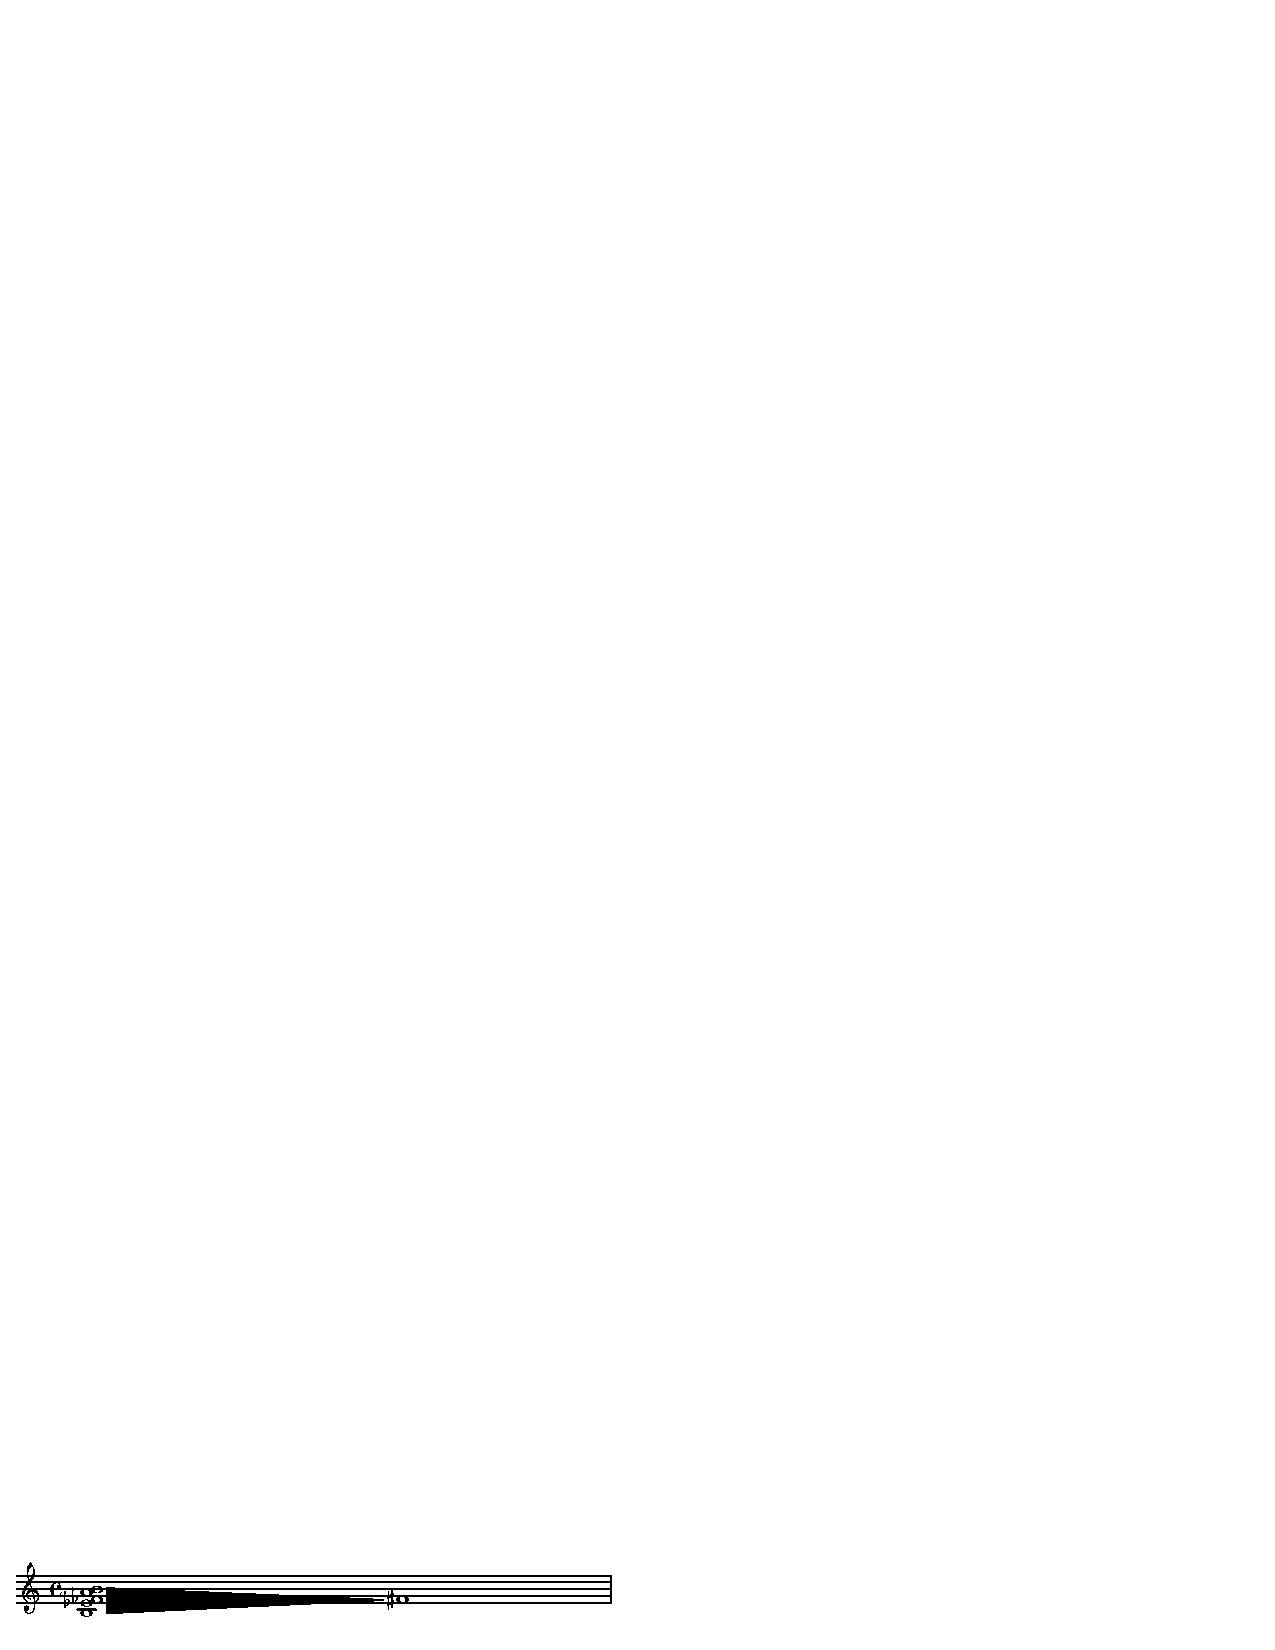
\includegraphics[width=0.75\textwidth]{img/ethsnd/chord}
\caption[Harmony for \emph{etherSound}: Instrument B]{Harmony for Instrument B as a result of the message
  ``\emph{Hello, my name is Henrik.}''.} \label{chord}
\end{center}
\end{figure}

The initial pitches are derived from the occurrence of certain key letters in the originating text.\footnote{For the sake of experiment   and variation, I am changing these 'key notes' for every performance   of \emph{etherSound}.} The first unique occurrence of one of the key letters, searched for from the first letter of the word corresponding to the current voice until the end of the message, becomes the initial pitch for each voice. If none is found, the voice is deleted. The voicing of the initial chord is constructed so that the first voice will be the top note of the chord and consecutive voices will be laid out below this using octave transposition, aiming for the closest possible voicing. 
The exact micro-tonal centre pitch between the highest and lowest note of the initial chord is then calculated (this would be the pitch `D' if the initial chord is a major third up from `C'). After the initial chord has been introduced, all voices begin a virtual glissando toward the centre between the outer limits of the chord, creating micro-tonal variations, ending at a unison.\footnote{The same technique is used in   the composition \emph{Drive} (2003). The score for \emph{Drive}   shows the notation of the instantaneous (approximate) harmony at five consecutive points in time, ending at a B quarter of a tone   sharp.} For each excitation of each voice, the instantaneous value of the corresponding glissando sets the pitch for that excitation. The message from Table \ref{time} would result in the chord shown in Figure \ref{chord}---the initial chord and the glissandi towards the centre pitch---if the max polyphony value is set to five or higher and the `key' characters are mapped by German note names (a to A, b to Bb, c to C, ... ,h to B and s to Eb). 
The timbre of the voices played by this instrument is shaped by the vowels contained in the message and the order in which they appear. For non-real-time processing this is achieved by synthesising the first five formants of the first vowel found in the word corresponding to the current voice and then interpolating between the formant spectrum of the remaining vowels of the message (see Table \ref{vowel}). As this method is very expensive---it requires allocation of five times as many voices---a cheaper alternative was used in the first real time versions of \emph{etherSound}. By modulating the formant centre frequency of one single FOF voice using frequency modulation with the carrier and index signal frequencies derived from the vowel interpolation described above, the effect of moulding the spectrum in a way related to the content of the message is retained. In the latest version the two methods are combined in order to achieve a greater sonic variation---all five formants are synthesised for every note and the formant centre frequencies of some of the notes are also modulated. 
\subsection{Sound event generation and synthesis---conclusion} The two instruments offer different interpretations of the message played back in parallel. As Instrument A performs a linear displacement within the message, Instrument B gives a snapshot image of the entire text at once, an image which gradually dissolves over time. Metaphorically speaking, one instrument is modelling the discrete words and characters as they appear in time, the objective flow of the components of the message, and the other deals with the continuous meaning, or subjective understanding, of the message as it is interpreted in its entirety. Although the result can be rather complex and abstract it is my intention that certain conceptual elements of the input should be retained in the output. In the following section I will reflect on the issue of interaction within the context of \emph{etherSound} and to what extent my intentions of input-output correlation can be said to have been fulfilled. 

%\newpage
\begin{landscape}
\centering
\begin{table}[!pt]
\begin{tabularx}{\linewidth}{|p{.8in}|X|X|X|X|X|X|X|X|X|X|X|X|X|X|X|X|X|X|X|X|X|X|X|X|X|}
\hline
&H & E & L & L & O &,& &M&Y& &N&A&M&E& &I&S& &H&E&N&R&I&K&.\\
\hline
\textit{bar}&\multicolumn{7}{|l|}{1} & \multicolumn{3}{|l|}{2} & \multicolumn{5}{|l|}{3} & \multicolumn{3}{|l|}{4} & \multicolumn{7}{|l|}{5}\\
\hline
\textit{beats per bar}&\multicolumn{7}{|c|}{3} & \multicolumn{3}{|c|}{1} & \multicolumn{5}{|c|}{2} & \multicolumn{3}{|c|}{1} & \multicolumn{7}{|c|}{3}\\
\hline
\textit{subdivision}&\multicolumn{2}{|c|}{2} & \multicolumn{3}{|c|}{3} & \multicolumn{2}{|c|}{2} & \multicolumn{3}{|c|}{3} & \multicolumn{2}{|c|}{2} & \multicolumn{3}{|c|}{3} & \multicolumn{3}{|c|}{3} & \multicolumn{2}{|c|}{2} & \multicolumn{3}{|c|}{3} & \multicolumn{2}{|c|}{2}\\
\hline
\textit{accents}& & \textgreater & & &\textgreater & & & & \textgreater& & & \textgreater& &\textgreater & &\textgreater& & & & \textgreater& & &\textgreater&\textgreater& \\
\hline
\end{tabularx}
\caption[Rhythmic distribution of notes in Instrument A.]{Rhythmic distribution of notes in Instrument A. Influence of vowels on four consecutive voices of Instrument B.} \label{time}
\end{table}

\centering
\begin{table}[!pt]
\begin{tabularx}{\linewidth}{|p{.8in}|X|X|X|X|X|X|X|X|X|X|X|X|X|X|X|X|X|X|X|X|X|X|X|X|X|}
\hline
&H & E & L & L & O &,& &M&Y& &N&A&M&E& &I&S& &H&E&N&R&I&K&.\\
\hline
\textit{voice 1}&\multicolumn{3}{|c|}{E} & \multicolumn{3}{|c|}{O} & \multicolumn{3}{|c|}{Y} & \multicolumn{3}{|c|}{A} & \multicolumn{3}{|c|}{E} & \multicolumn{3}{|c|}{I} & \multicolumn{3}{|c|}{E} & \multicolumn{4}{|c|}{I}\\
\hline
\textit{voice 2}& \multicolumn{4}{|c|}{Y} & \multicolumn{4}{|c|}{A} & \multicolumn{4}{|c|}{E} & \multicolumn{4}{|c|}{I} & \multicolumn{4}{|c|}{E} & \multicolumn{5}{|c|}{I}\\
\hline
\textit{voice 3}& \multicolumn{5}{|c|}{A} & \multicolumn{5}{|c|}{E} & \multicolumn{5}{|c|}{I} & \multicolumn{5}{|c|}{E} & \multicolumn{5}{|c|}{I}\\
\hline
\textit{voice 4}& \multicolumn{8}{|c|}{I} & \multicolumn{8}{|c|}{E} & \multicolumn{9}{|c|}{I}\\
\hline
\end{tabularx}
\caption{Influence of vowels on four consecutive voices of Instrument B.} \label{vowel}
\end{table}

\end{landscape}

%%% Local Variables: 
%%% mode: latex
%%% TeX-master: "../ImprovisationComputersInteraction"
%%% End: 

\section{Discussion and reflection} 
As already explained, the main issue for \emph{etherSound} is to allow for unconditioned participation. I was more concerned with the collection of diverse input than I was with giving the contributor a sense of control or participation, and in the first versions of \emph{etherSound} the message-compositions were much less dependent on input than they are in the current version. My grounds for changing this, and in the current version letting the messages generate a musical event with a clear form, stem from the wish to retain a perceptible connection - even though this connection may only be dismantled by the \emph{change} in output - between input and output. 
The process of designing the analysis and synthesis programs described above is to a considerable extent tantamount with the process of composition in the traditional sense. In a sense, \emph{etherSound} is an algorithmic or ruled-based composition\footnote{French composer Michel Philippot and Italian composer Pietro Grossi were pioneers of algorithmic composition.} with stochastic elements, methods which have been explored by many composers for many years. In his book \textit{Formalized Music} composer Iannis \citeauthor{xenakis71} offers a thorough investigation of the concept of stochastic music which came about as a reaction to post-serialistic music:

\begin{squote}
 For if, thanks to complexity, the strict, deterministic causality which the neo-serialists postulated was lost, then it was necessary to replace it by a more general causality, by a probabilistic logic which would contain strict serial causality as a particular case.\footcite[8]{xenakis71}
\end{squote}

Whereas in the case of Xenakis, however, the results of the stochastic processes were strictly encoded into a score or a computer program, in \emph{etherSound} there is no score as such. The mapping between characters in the input, and synthesis and sequencing parameters used to produce the output, is fixed in the program but no sound will be produced unless someone takes the action to provide the system with input. John Cage's non-deterministic music based on chance operations is another example in which events in some regard external to the composer are allowed a great influence on the final result. Cage's aesthetics were a means to remove \textit{intention} from the artistic expression. On the face of it there may be a conceptual resemblance between \emph{etherSound} and the non-determinism of Cage. In \emph{etherSound}, however, it is precisely \textit{intention} that produces sound: the wish to participate is all that is needed. 

The choices that had to be made in the mapping of input to output in the program are the same kind of choices I make when I compose or improvise. I would call these compositional choices. They are based on my musical experience and what it is I want to achieve---for whatever reasons---at any particular moment. The process of making these choices in the context of developing and designing interactive systems is well described by Camurri and colleagues: ``The designer of the performance introduces sound and music knowledge into the system, along with the compositional goals [\ldots]''.\footcite[Camurri, Richetti, and Trocca, 1999, as cited in][373]{rowe01} This fact, that compositional choices were made in the course of constructing \emph{etherSound}, does not necessarily make it into a `composition'. Before we ponder more on the identity of \emph{etherSound}, however, what is the nature of its driving force, the interaction between the program, the \index{performer}performers and the participants? In what sense is \emph{etherSound} interactive? If the mapping is fixed in the program, what is the influence of the participant? 

\subsection{Interaction in \emph{etherSound}}
\label{sec:inter-emph}

\emph{etherSound} has been used in two different contexts: as a standalone sound installation that users can interact with but also in combination with one or several improvising musicians playing acoustical instruments. The discussion that follows will primarily deal with the latter situation, which resembles a traditional concert but one in which the audience, apart from listening, may also `play' the electronic instrument. As can be gathered from the description of the system given above, the sonic outcome of a received SMS is fairly strictly pre-conceived. On the individual level, only a limited amount of influence over detail is offered, and it is debatable whether \emph{etherSound} can be called an `instrument' at all. 
%%% Why would we like to call etherSound an instrument? %%%
This was, however, never the intention. It is the \emph{desire} to contribute to the whole that was intended to be the ruling factor, not the individuality of expression or the virtuosity of performance. But in that case, why not simply have a button that the users can press at will which generates a pseudo-random sequence of sonic events? Surely, this too would allow for unconditioned participation.
 
In the very first performance of \emph{etherSound}, on the day of the opening of the exhibition \emph{The Invisible Landscapes} in August 2003, and owing to a technical problem,\footnote{The problem was owed to an unknown inconsistency in how JSP (Java Server Pages), which I used on the server to parse the messages, handled HTTP/POST requests when the version of the HTTP differed between the caller and the receiver.} as an emergency solution I implemented a version which basically worked like a button. I was unable to parse the actual contents of the SMS messages sent to the system (I merely obtained a notification that a message had been received). Rather than cancel the performance I had the program read an arbitrary number of words from a text file on my hard drive and use that as a `fake' message. Still, in the information about the installation and in the program notes for the concert, all of which had been prepared well in advance, it was stated that the system responded to the contents of the message when composing its output. After the concert a few of the listeners/participants came up to me and told me how clear they thought the connections between the SMS contents and the sounds were. The expectancy of a correlation between input and output was so strong that, despite the fact that the actual mapping was completely random, the connection was created in the perception of the participant. This is not to say that `faking' interaction is a practicable solution, but merely that expectation, and hence information about (modes of) interaction, is an important factor. 

\emph{etherSound} is not interactive in the same way that, for example, a computer game is interactive. Once the SMS has been sent, there is no way for the participant to alter or influence the sound. There is correlation between input and output insofar as short messages produce short message-compositions and vice versa. After sending a few messages, or after listening to a series of message-compositions, the participant will know what to expect and the ease of use is perhaps the greatest advantage of \emph{etherSound}. Interaction in the context of computers and technology is more or less synonymous with \textit{control}, or with the ability to change the prerequisites during the course of action. As put by George \citeauthor{lewis00}: ``interactivity has gradually become a metonym for information retrieval rather than dialogue''.\footcite[36]{lewis00}
%%% What about 'dialogueâ' in etherSOund... Is there real dialogue? %%%
Computer programs that are not interactive perform a task based on the information given to them at the outset. In interactive computer programs the parameters can be changed dynamically. By this definition and if we restrict the time frame to one message-composition, \emph{etherSound} is not really interactive or only interactive in a very limited sense. It does not allow the user to dynamically control the musical contour of the message-composition. It is more of a stochastic jukebox whose `play' button works by means of sending an SMS. 

If, however, we expand our understanding of interaction and include readings that are more closely related to \index{interaction!social}social interaction, which is not about control, but about exchange, about giving and taking, and about growing and establishing identity,\footnote{The role of social interaction in human existence has a long philosophical history, in recent years kept alive by Hannah Arendt and J\"{u}rgen Habermas. This is discussed in more detail in Chapter \ref{sec:interraction-self}.} and we expand the time frame to include a series of message-compositions, we can come up with another analysis. If our general requirement for the definition of interaction is not limited to the subject's unbounded control over content (``information retrieval''), and the context-specific requisite for interaction is not restrained to the participant-\index{interaction!computer}computer interaction, but also includes participant-participant and participant-performer interaction: then \emph{etherSound} may well be said to manifest a form for dynamic interaction and the users who interact with it do indeed have influence.
%%% IS interaction the same as influence? %%%
In a recent performance (Copenhagen, August 2007) a participant sent a message that ended the concert. Whether that was intended or not is less important than the actual consequence. The participant introduces a change in the musical context and, though he or she does not control the outcome of this change, the participant still in effect has the power of influence (influence rather than control) through interaction. 

What then are the consequences regarding interaction that may be drawn from working with \emph{etherSound} in the context of performance? If we begin by thinking about this piece as an improvised live performance, on an individual level the system \emph{etherSound} provides the ability for any member of the audience (who by virtue of being a part of the audience is already interacting with the performance) interactively to introduce a change to the sonic environment at any point, albeit with a very limited control over the outcome. Now, from my elevated perspective as a musician with fifteen years of professional experience I am in no position to tell what this situation means to someone who has never before participated in an improvised musical event. It may be incredibly dull or it may be the most exciting sensation. For me, as an improviser, the interaction as it is taking place here supplies that which the computer does not (and never will be able to?) possess---the intention. The message-compositions are not dispersed randomly (as in a pseudo-random computer algorithm) but because someone wanted to participate. 
%%% To me this sounds a bit like our voting system. There is an intention on the part of the voter, there even might be some kind of influence. However, s/he has no idea at all what s/he will get after the elections %%%
When I was playing and I heard the sounds of a message-composition I felt honoured that someone had taken the time to participate, and it felt as though I had been given a gift.\footnote{The `gift' aspect is further discussed in \cite{frisk05} and \cite{yoshida06}.} Though the idea that the participation would supply me with a non-predictable, but not random, series of impulses, was part of the original conception of \emph{etherSound}, I had not anticipated the impact it would have on me. It is not easy to make general assumptions regarding interaction, but to me this shows the importance of moving beyond interaction as a deterministic mapping of stimulus to response.
% , to let both parties involved in the interaction create the object of interaction in order to intend it. %%% But is this determinism interaction? %%%

There are a number of different kinds of interaction going on in a performance of \emph{etherSound}, on many different levels. There is the low-level interaction between the participant and the computer mediated through the mobile phone as well as higher levels of interaction between groups of participants and groups of \index{performer}performers. To summarise, in order to appreciate the nature of the interactive potential for \emph{etherSound} (i) time needs to be considered, (ii) expectation is an important factor, and (iii) information \emph{about} the processes taking place as a result of interaction (`meta-information' or the `grammar' of interaction) is absolutely essential. 

%%% More general remarks after reading thus far: Go deeper into the topic of interaction. E.g. (1) What about the difference between musician-composer, participant-composer, participant-musician? (2) Is intention a prerequisite for interaction and is therefore no real interaction possible with a computer? %%%

\subsection{The work identity of \emph{etherSound}}
\label{sec:ident-emph}

The question of the work identity is not merely a theoretical issue in this context of purely scholarly import. If the intention of \emph{etherSound} was to create an open-ended platform for public participation with a focus on interaction and, in the end, the result has more in common with a composition for instruments and computer, not only did the intention fail (which may be perfectly all right), but my personal objective, to use interaction as a way to open up the creative process and give up compositional control, failed. The latter may also be all right, but if in the long run there is a continuous discrepancy between artistic intentions and practical results this is likely to create personal and artistic frustration. 

Given the different agents involved in the production of musical content in \emph{etherSound}, the most obvious perspective to adopt (given that we are talking about message-compositions) is that the participants are the composers and the computer with the improvising musicians are the \index{performer}performers. This would make the SMS the score(s). Musicologist Peter \citeauthor{kivy02} gives a definition of the musical score as ``a complex symbol system. From the performer's point of view it is a complex set of instructions for producing a performance of the musical work that it notates''.\footcite[204]{kivy02} Applying this definition to \emph{etherSound}, we may extract (at least) two other plausible explanations of its structure:
%
\begin{enumerate} 
\item If the participants (SMS senders and improvising musicians) are the \index{performer}performers, the instructions, the meta-information or the `grammar' of the interaction constitute \emph{a} score. 
\item If the computer is the performer (which would turn the participants into quasi conductors) the computer program, i.e. the code in which the mapping between input and output is defined, would constitute another \emph{version} of \emph{a} score. \end{enumerate}
%
According to the definition given, even if we regard the work from two or three different perspectives, there is a score. 
%%%The interesting point you’re coming at is that etherSound makes use of a singular score which seems like a kind of paradox %%%
If in fact there is a score of some sort in which the mapping is fixed and not subject to change through interaction, and if the process of building this mapping scheme is similar or even equal to compositional processes, in what sense does \emph{etherSound} differ from a composition? First of all, Kivy's definition is clearly by no means conclusive. Second, there is an important difference between a more traditional composition and a work such as \emph{etherSound} in the dimension of time, as the latter does not have a fixed beginning or an end. Last, and most important, between the two contrasting musical work concepts `closed' or `pre-conceived', and `open' or `free' there is a range of possibilities, and, as with so much other music and art, depending on \emph{when} and \emph{how} you look at the piece it will define itself at different points on the open-closed axis. \emph{etherSound} exists in this field ranging from the closed form of a message-composition to the openness of the large scale form of the improvisation. 

More than anything else \emph{etherSound} is an improvisation. The structure or the `language' for the improvisation may be different depending on your role, and the `score' (if it exists) is ``a recipe for possible music-making''.\footcite[Evan Parker, as cited in][81]{bailey92} The compositional choices discussed above are a part, for this piece a necessary part, of the structure that makes possible the different entry points. Systematic and pre-conceived construction in one phase of a musical project does not have to limit the performative freedom or result in a closed `work'. On the contrary (and perhaps in opposition to the romanticised view on improvisation), preparation for an improvised performance, even in free form jazz improvisation, is quite often highly structured and systematic. Improviser and jazz saxophonist Steve Lacy has the following recollection of the early years of Cecil Taylor's career:\footnote{It should be pointed out that I make no comparison between \emph{etherSound} as music and the music of Cecil Taylor.} ``And the results were as free as anything you could hear. But it was not done in a free way. It was built up very, very systematically [\ldots]''.\footcite[Cited in][81]{bailey92} Further, construction and pre-conception on the detailed level do not exclude that the whole is still open and self-generated: ``[E]ach of the numerous released recordings of, say, Coltrane's `Giant Steps,' regarded at the level of individual passages, is the result of careful preparation [\ldots]. At the same time, each improvisation, taken as a whole, maintains its character as unique and spontaneous''.\footcite[108]{lewis-1} In both the recordings of \emph{etherSound} (2003 and 2007) the common `language' of the performing musicians is their background as jazz improvisers.
%%% So, the interaction goes in fact one way: it’s just a matter of seducing the performer (you) %%%
The language of the participants is the text and logic of SMS messages and the intention to participate is what binds the two together. 

To conclude this discussion I would like to turn again to George \citeauthor{lewis-1}, who, I believe, captures the essence of how form and structure are developed in improvised music: 
\begin{squote} 
My own view is that in analyzing improvisative musical activity or behaviour in structural terms, questions relating to how, when, and why are critical. On the other hand, the question of whether structure exists in an improvisation---or for that matter, in any human activity---often begs the question in a manner that risks becoming not so much exegetic as pejorative. It should be axiomatic that, both in our musical and in our human, everyday-life improvisations, we interact with our environment, navigating through time, place, and situation, both creating and discovering form. On the face of it, this interactive, form-giving process appears to take root and flower freely, in many kinds of music, both with and without preexisting rules and regulations. \footcite[117]{lewis-1} 
\end{squote} 
From my personal thinking about the work identity of \emph{etherSound}, I have gone full circle. At the outset I thought of it as nothing but a framework for improvisation in which I could allow myself to experiment with using the computer in a way distinctly different from what I was used to. Then, for many reasons, one of which was the fact that it is precisely not \emph{axiomatic} that form may be created as well as constructed, I went into a phase of denial, in which I sought for a structure that would allow me to call \emph{etherSound} a `work', only in the end to arrive at the conclusion that what it is, first and foremost, is an improvisation. 

%%%
%%% General remark: With whom is the audience actually interacting? (1) With the musicians on stage; (2) With etherSound; (3) With a computer; (4) With their cell phones; (5) With music (sounds)????? 
%%%

\section{Summary}
\label{sec:endnote}

Whether or not the participants felt they had influence and whether this influence set creative energies in motion within the participant can only be proved, if at all, by performing empirical and statistical studies that are beyond my intentions and competence. What I can do, however, is reflect on my experiences of performing \emph{etherSound} on a number of occasions. From my experiences as a performer---from that perspective---I can say that the participants were truly interacting with the music and they had genuine influence on the development of the performance. As an improviser in the context of a performance, I experience no difference between an initiative taken by one of the other musicians or one introduced by a participant---they are of equal import. 
%%% Perhaps of equal import but at least the action-reaction among musicians continue and develop (deepen) %%%
Though I have programmed \emph{etherSound} myself, enough musically crucial aspects of the message-composition are unknown at the outset for any message-composition to hold potential for musical change. Obviously, the nature of the interface and the way the piece is programmed put great limitations on the creative possibilities of the participants, especially were they to work with it repeatedly. That, however, does not mean that the individual, single act of participating does not harbour creative and interactive potential. Just as I, when improvising, cannot be certain how a musical initiative taken by me will influence the development of the music, so the participant will not know either. 
%%% Is that really the same thing for you? %%%
Still---just to be absolutely clear about what it is we are talking about---sending an SMS to \emph{etherSound} during a performance is obviously nothing like, not even closely related to, improvising on an instrument one has learned and mastered. This is not, however, the point I am trying to make. The point I am making by this long detour of reflection is that perhaps---and my own experience seems to corroborate this---a tiny atom of that which constitutes the essence of, at its best, flowering, form-giving process of improvisation, to use the words of George Lewis, can be shared by those whose participation is restricted to a mobile phone.
%%% Is this your main conclusion? %%%

In musical improvisation the more I play with and get to know my co-improvisers, however, and now we are approaching the weak spot of \emph{etherSound} as a platform for interaction, the easier it will be to predict the result of musical actions taken. For the participants there are currently only very limited possibilities for this kind of development to take place. Developing the expert performance aspect of a work whose objective is related to a notion of `equality of participation'---that all, regardless of prior (musical) training, should be allowed an equal chance to participate---is not un-problematic. If this goal is to be adhered to care must be taken not to accomplish the expert performance aspect at the expense of un-initiated participation. Adding a second layer of interaction would be one way to allow the interested participant to acquire the skills to take part in a performance more actively and consciously. This second layer could be implemented by making a phone call and interacting with the message-composition---changing the volume, the timbre, the tempo, etc.---in \index{real-time}\index{time!real-time}real time, either by pressing digits on the phone or by voice control. 

In \emph{etherSound} in the performance context the audience is invited to take part in a group improvisation. Though the \emph{\index{interaction!as control}\index{interaction-as-control}interaction-as-control} aspect of the participation is very limited the interactive action influences the music in a similar way to \index{interaction!musical}musical interaction in the context of improvisation. 
%%% I think I don’t agree (see previous remark) %%%
To summarise my own experiences of working with this project over a number of years, I can say that the sensation of improvising in a context where the audience can give sonic input---input that becomes an important part of the performance---is very rewarding, to an extent that I did not anticipate at the time the project started. A challenge for future development of the concept, though the artistic implications of such development have to be carefully evaluated, would be to develop the participant control aspect of the interface without losing the collaborative focus.


%%% So, what did etherSound teach you about the relation computer-music-interaction? What can you conclude in more general terms that will benefit not only your own artistic work but also others? %%%

%%% Local Variables: 
%%% mode: latex
%%% TeX-master: "../ImprovisationComputersInteraction"
%%% End: 


\chapter[Repetition]{Repetition Repeats all other Repetitions}
\label{cha:repe-main}
\hspace{6.5cm}

% \begin{wrapfigure}{r}{0.4\linewidth}
%   \begin{minipage}[h]{\linewidth}
%     \musicannot{Repetition Repeats all other Repetitions\\\emph{for 10-stringed guitar and computer}\\Composed \& premiered in 1996 \\Commissioned by and dedicated to Stefan \"{O}stersj\"{o}}
%   \end{minipage}
% \end{wrapfigure}

\begin{wrapfigure}{r}{0.45\linewidth}
  \begin{minipage}[h]{\linewidth}
    \begin{flushright}
      \musicannot{Repetition Repeats all other Repetitions\\
        \emph{for ten-stringed guitar and computer}\\
        Composed \& premiered in 2006\\
        Commissioned by and dedicated to Stefan \"{O}stersj\"{o}}
    \end{flushright}
  \end{minipage}
\end{wrapfigure}

%%% Local Variables: 
%%% mode: latex
%%% TeX-master: "../ImprovisationComputersInteraction"
%%% End: 


% \vspace{1cm}
\noindent In this chapter the work-in-movement \emph{Repetition Repeats all other Repetitions} and the context from which it came into being are discussed. Although the text here summarises the two essays \citetitle{frisk-ost06} and \citetitle{frisk-ost06-2} some of the thinking here depends on those texts. Just as those two essays were co-written with Stefan \"{O}stersj\"{o}, the guitarist who commissioned \emph{Repetition}, the current chapter is largely based on a co-written text.\footcite[Another version of the original text is part of his PhD thesis. See][]{ostersjo08} Owing to the collaborative nature of the project, and to avoid tedious repetitions, throughout the text I refer to Stefan by his first name only and when I use `we' and `us' I consistently refer to Stefan and me. The primary purpose of the studies within \emph{Negotiating the Musical Work}\footnote{See \fullcite{frisk-ost06}; and \fullcite{frisk-ost06-2}} was to understand musical collaboration and composer-performer interaction better but already in the first study it became clear to us that much of the knowledge could equally well be used in terms of musician-computer interaction, which, to me, was emerging as the more interesting aspect of these studies. These ideas contributed strongly to the emergence of the idea of \index{interaction!as difference}\index{interaction-as-difference}interaction-as-difference as well as the giving up of the \index{Self}Self.


In order to unwrap the processes that led to the first version of \emph{Repetition Repeats all other   Repetitions}\footnote{Henceforth referred to as \emph{Repetition}.} and eventually to the expanded concept of the `open work', it should be clear that many circumstances, some of which are auxiliary to the actual process of 'composing' (i.e. the tasks traditionally assigned to the `composer') had a great influence on the way the piece developed. In the end, however, it turned out that these 'circumstances' or 'processes' were not in fact 'auxiliary': They were, or would become, an integral part of the process of composing (now also in the extended sense of the term). Some of these were planned and others came about as a result of the ways in which the project developed. For example, one of the outspoken intentions was to use \emph{Repetition} as a testbed for my timbre tracking \index{software}software \emph{timbreMap} (see \ref{sec:timbremap}), and one of the perhaps more unexpected consequences was the formation of a new group, \emph{\useGlosentry{glos:six-tones}{The Six Tones}}, which can be seen as a direct consequence of the collaboration Stefan and I had initiated in January 2006. Not only an offspring of our collaboration \emph{The Six Tones}, as is often the case with multi-project collaborations, also provided important material for \emph{Repetition}. A timeline of some of the more important events relating to this project may be gathered from Figure \ref{fig:repetition-timeline}, and below I give an account of the development of the piece---and the development of the project---and the circumstances that, according to my own biased view, were the most important ones to shape the piece (i.e. most important with regard to the theme of this book). It should, however, be clear to the reader that the process of composing, or constructing, \emph{Repetition} has not yet come to an end, but continues to feed material and events into the `container' that \emph{Repetition} has come to represent. In its first conception, although the \emph{project} was thought of as collaborative, the \emph{music itself}---the score and its performances---was not. But the stream of events born out of the process shaped \emph{Repetition} as a truly collaborative effort, in which the members of the collaboration were no longer limited to myself and Stefan \"{O}stersj\"{o} and me. Some of these events are described in the following sections and may be summarised as:

\begin{enumerate}[(1)]
\item \textbf{Negotiating the Musical Work} That Stefan \"{O}stersj\"{o} and I had mutually agreed on \emph{Repetition} being part of my own, as well as his, doctoral research project is an important factor that, in the end, greatly influenced the result. In particular the preparatory studies and the papers we wrote as a result had impact on the development of the project.% %$|$\hyperref[sec:negotiating-1]{here}
%
\item \textbf{The Six Tones}\footnote{As is more fully explained in Section \ref{sec:negotiating-2} \emph{The Six Tones} was composed for a newly formed Vietnamese-Swedish quartet that later takes its name from the title of the composition \emph{The Six Tones}.} Working with \emph{The Six Tones} added other kinds of instrumental and sonic input and it intensified the social aspect of our collaboration owing to the additional work relation. There is also a close intertextual relation between my piece \emph{The Six Tones} and  \emph{Repetition} in that each contains transcriptions of the other. %$|$  \hyperref[sec:negotiating-2]{here}
%
\item \textbf{The first version} A combination of events, decisions and circumstances led to the decision \emph{not} to employ `true' interactivity in the first version performed in October 2006. This radical conclusion gave birth to the idea of \emph{Repetition} as a piece that can have many independent instances.% $|$  \hyperref[sec:negotiating-3]{here}
%
\item \textbf{Symphonie Diagonale} The next version would be even less \emph{\index{real-time}\index{time!real-time}real-time} interactive and even \emph{more} collaborative and this time had already been performed a number of times. %$|$\hyperref[sec:negotiating-4]{here}
%
\item \textbf{The annotated score} Although primarily concerned with `preservation' (see the section on \hyperlink{sec:target:libintegra-1}{libIntegra in the Introduction}), working with the Integra project\footnote{See \url{http://www.integralive.org} and \cite{frisk-bull07,frisk-bullock08}.} made me start thinking of a representation of the \index{ontology}ontology of a musical work as a possibility for a documentation of the `work in motion'; this being the kind of work with which Stefan and I would associate \emph{Repetition}.% $|$  \hyperref[sec:negotiating-6]{here} 
\end{enumerate}

\begin{figure}[htb]
  \centering
  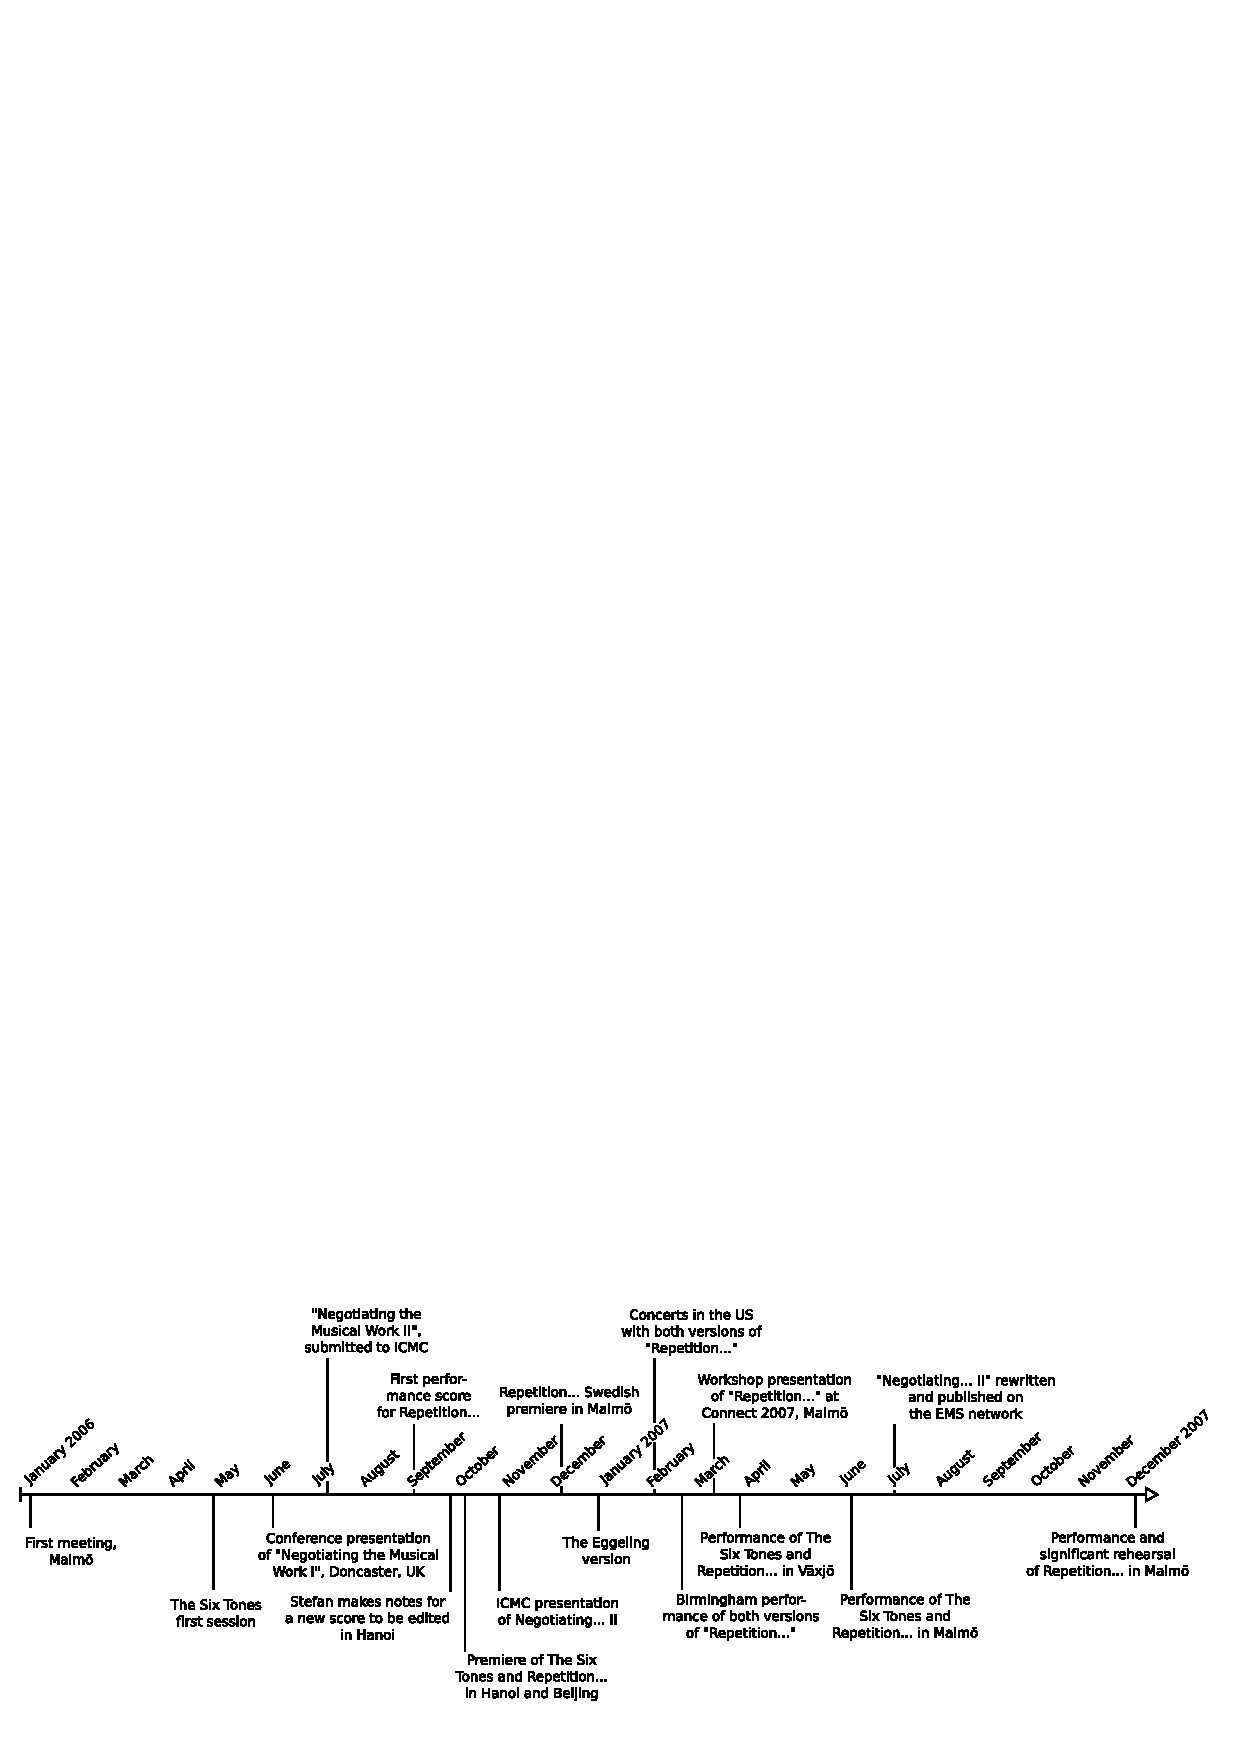
\includegraphics[width=\textwidth]{img/Repetition-timeline}
  \caption[Time line of events relating to \emph{Repetition\ldots}]{The events mapped on a time line relating to the life span of \emph{Repetition Repeats all other Repetitions}.}
  \label{fig:repetition-timeline}
\end{figure}

%\marginpar{\listoftags{\tagword{Repetition}, \tagword{timbreMap},
%\tagword{Negotiate}, \tagword{Semiology} }}

\section{Observing negotiations of the musical work}
\label{sec:negotiating-1}

\begin{wrapfigure}{r}{0.4\linewidth}
  \begin{minipage}[h]{\linewidth}
    \begin{flushright}
      \musicannot{Negotiating the Musical Work\\
        \emph{video analysis of a composer-performer session}}
      \end{flushright}
  \end{minipage}
\end{wrapfigure}

%%% Local Variables: 
%%% mode: latex
%%% TeX-master: "../ImprovisationComputersInteraction"
%%% End: 

Part of our agreement, and perhaps a first prerequisite for any successful composer-musician collaboration, was the idea of partly giving up the traditional view of our respective roles.\footnote{This process belongs to the notion of giving up the \index{Self}Self.} We would each allow ourselves to enter the domain of the other and we would allow each allow the other to enter our own professional sphere. In one of the earliest results of this project---the documentation of a study of a collaboration similar to ours, between Stefan \"{O}stersj\"{o} and Swedish composer Love Mangs---we had seen an example of this behaviour.\footcite{frisk-ost06} In the analysis of the video documentation of their collaboration, from which we had chosen a few excerpts, there were moments when Mangs was giving input to the process ``as if'' he was interpreting the material and moments when Stefan was manipulating the material ``as if'' he was the composer. I say ``as if'', because although the project was an outspoken collaboration in which the two musicians would meet and work out the material together, it is noted in the analysis that  Love Mangs in particular was not entirely comfortable with the floating nature of his identity as composer.

In the study \emph{Negotiating the Musical Work}, in an attempt to build an experimental framework to be used to unwrap these processes, we discuss the semiological model for musical analysis by musicologists Jean-Jacques Nattiez and Jean Molino. Their model looks at the work of art as an object that may be analysed from three different perspectives or levels: ``the poietic, the esthesic and the `neutral''.\footcite{molino} Three modes all representing the same work of art where the \useGlosentry{glos:poietic}{poietic} level is the constructive phase, the \useGlosentry{glos:esthesic}{esthesic} is the interpretative phase and the neutral is the trace left by the poietic (or esthesic) process\footcite{molino}\nocite{molino2}. At the time, this tripartite model was the object of some excitement to Nattiez, who believed that 
%%
\begin{squote}
[\ldots] recognizing, elaborating, and articulating the three relatively autonomous levels (\useGlosentry{glos:poietic}{poietic}, neutral and \useGlosentry{glos:esthesic}{esthesic}) facilitates knowledge of all processes unleashed by the musical work, from the moment of the work's conception, passing through its `writing down', to its performance. \footcite{nattiez}
\end{squote}
%%

\label{sec:1-par:2}
For perhaps obvious reasons the musical semiology proposed by Nattiez has been criticised and discussed widely, and it is not my intention to engage in that somewhat dated debate here.\footnote{The   concept of the `neutral analysis' or `analysis on the neutral level'   is particularly troublesome. For an insight in the debate from both   sides, see \cite{nat89} and \cite{dunsby83}.} Nevertheless, the terminology of Nattiez and Molino proved to be useful to us. Our adaptation of it, in particular the two levels \emph{poietic} and \emph{esthesic}, helped us reconsider the traditional division of labor between `musician' and `composer'. Whereas Nattiez lean on semiology in order to confirm the authority of the composer as the creator of the work (with the interpreter `inserted' towards the end of the poietic process\footcite[See][73]{nattiez}), we used it to depict what we analysed as a rather rapid oscillation between poietic and esthesic processes, and whereas Nattiez in his book \citetitle{nattiez} is primarily concerned with the composed \emph{work} and its \index{ontology}ontology, we focused on the interactions involved in the phases \emph{prior} to the existence of a score and prior to the first performances. The process of writing down a musical work, we argue, is not a unidirectional poietic process, but is described by us as an \emph{interaction} between esthesic and poietic processes, to an extent that makes it difficult to define the end of one and the beginning of the other. What Stefan and I attempted to show in the studies mentioned above is that the acts of musical composition that Nattiez gathers within the poietics can in themselves be analysed by using the same method that he applies to the total fact of the musical work. Nattiez seems to be drawing conclusions about ``processes unleashed by the musical work'' from a purely analytical understanding of music, from a perspective still dependent on the view of composers as `true creators' and works as `ideal objects' (in the phenomenological sense); stable and fixed artworks that should make up the primary object of study for musicology. What we were concerned with then, and what I am concerned with here, is almost the opposite: at least we are operating on the other side of the dividing line constituted by the completed score, the musical work as a coherent object, namely prior to the existence of a score and prior to the performance. Our concern is to attempt to understand the actions that \emph{lead to} musical content and the significance of the interactions between the agents involved in these processes, and to investigate the meaning of collaboration in the musical \emph{poesis} and the significance of these processes with regard to the technological \emph{poesis} in musician-computer interactivity.

% \floatstyle{plain}
% \newfloat{Reflection}{H}{lop}[section]
% \begin{Reflection}
% \end{Reflection}

% Just as we found in our  study is there no such thing as 'only right % hemisphere' in  composing or improvising or programming. Nor does a % concept such  as 'inspiration' pertain to one hemisphere only. 

% Becoming: becoming saxophone, becoming computer 
% In the actual saxophone there is something of all the other things % that can become improvisation. That something is the virtual side.

\label{sec:1-par:3}
In Figure \ref{fig:timeline-mangs} we plot our analysis of the interaction between Stefan and Love Mangs. The activities (utterances, expressions, topics, etc.) are summarised by the white squares and the horizontal position of the squares shows who initiated the activity (Stefan on the right and Love on the left) and the mode (esthesic or poietic) with which we coupled it. The arrows pointing to and from the activity squares show the directionality of the communication and in the middle is an initiative curve, i.e. which of the two musicians holds the initiative at a given moment. Dashed lines in the communication arrows indicate a `noisy' or `dropped' message; a message that was misunderstood or not picked up by the other party. It should be noted that the graph is obviously a rough generalisation: the actual interaction between Stefan and Love Mangs was not so tidily square. Nevertheless, the graph shows an example of the non-linear and flexible character of their communication. From looking at the graph we can see that during this clip there is a tendency towards communicative clarity. At the top of the graph there is what seems to be a fair amount of confusion, a lot of individual activity not responded to (as is represented by the dashed lines of communication). Towards the bottom of the graph, however, the interaction is denser and appears to be less noisy, with the result that fewer messages are lost. In addition, as the composer in this session, Love Mangs is moving from being active almost exclusively in the esthesic domain to operating mainly in the poietic domain.\footnote{The analysis of the graph in Figure \ref{fig:timeline-mangs}---and of the events preceding it--- should only be seen as a summary. For a more complete and detailed discussion of the \"{O}stersj\"{o}/Mangs collaboration in general, see \cite[Chap.~3]{ostersjo08} and for a more in-depth analysis of the video clip discussed above see \cite[Sec.~3.2]{frisk-ost06} and \cite[Sec.~4]{frisk-ost06-2}.}

\label{sec:1-par:4}

The miscommunication, or rather the \emph{negotiation}, observable in the beginning of the session appears to play the role of a `tuning-in' between the two agents (see \hyperref[sec:timbremap]{Section \ref*{sec:timbremap}}), a tuning-in through negotiation that, towards the end of the session, allows the relations to become established in a way that permits creative decisions. One of the suggestions we make in \citetitle{frisk-ost06-2} is that Stefan and Love Mangs, in their negotiations, are defining a \emph{subculture}, against which the symbols \hyperref[fig:timeline-mangs]{in the graph} which represent ideas exchanged (e.g. the \emph{fermata} starting at line 45-65 or the \emph{arpeggio} roughly at line 145) derive their meaning. These thoughts lead us back to semiological thinking, though in a more general sense than that proposed by \citeauthor{nattiez} and \citeauthor{molino}. Umberto Eco claims that ``[a]ny attempt to establish the referent of a sign will force us to define this referent with the terminology of an abstract entity''.\footcite[66]{eco71} The signs, according to Eco, denote cultural entities which remain unaltered when the sign is transposed or translated. In this case, however, it is the abstract entity that is transposed in order to reveal the meaning of the symbol within this specific context. The \emph{fermata} in the example may or may not be related to the romantic idea of a fermata. Furthermore, there is likely to be a significance attached to the symbol that evades its immediate `meaning'. Both Stefan and Love Mangs are working within the frame of their own cultural contexts which define their respective understandings of the evolving work. The subculture, according to us, is a result of the interaction, and the negotiation (`\emph{What is it we are  developing?}', `\emph{How are we talking about it?}' etc.), between the two agents and their inherent cultural contexts. Their mutual expectations and their understanding or imagination of the work in progress is of importance when they attempt to co-ordinate their actions, for instance, towards a definition of the performance instructions. Where often the composer-performer relation is understood as a hierarchic structure in which the role, even the purpose, of the performer is to fulfil the composer's intentions, this mode of analysis allows us to look at the two agents (composer and performer) as part of a larger system that may also contain many other agents such as social and cultural context, instruments, status, power, gender, etc.

\label{sec:1-par:5}
To summarise the analysis of the Stefan and Love Mangs collaboration, it appears as if the noisy communication early on in the process did not halt the creativity. Ideas, including those that originated in these early and seemingly confusing negotiations, continued to develop while the agents involved slowly established a common space, a subcultural context. Against this context the symbols exchanged were given meaning, or \emph{new} meaning, in every respect different from the traditional meaning of the symbol. Assuming this analysis is correct---that noisy communication is not an obstacle to the establishment of common ground between communicating and collaborating agents---what does it mean to our understanding of computer-musician interaction in the context of \index{electro-acoustic music}electro-acoustic music? There is a tendency, not only in musician-\index{interaction!computer}computer interaction, but in \index{interaction!human-computer}\index{HCI}human-\index{interaction!computer}computer interaction in general, to look at the communication as primarily a one-way stream, in which noise in the transmission is a great problem. From the bottom up the computer is truly \index{digital}digital and it may be correct to let the input to such a system be binary. Looking at it, however, as an agent in a communicative system where binary distinctions are difficult to make and where the communication will be defined in the course of action, so to speak, will certainly present problems. Nevertheless, the study summarised above, and the results we reached in it, became the inspiration for the interactive model used in \emph{Repetition}.

% \begin{wrapfigure}{r}{10cm}
   \begin{figure}[ht]
    \begin{center}
       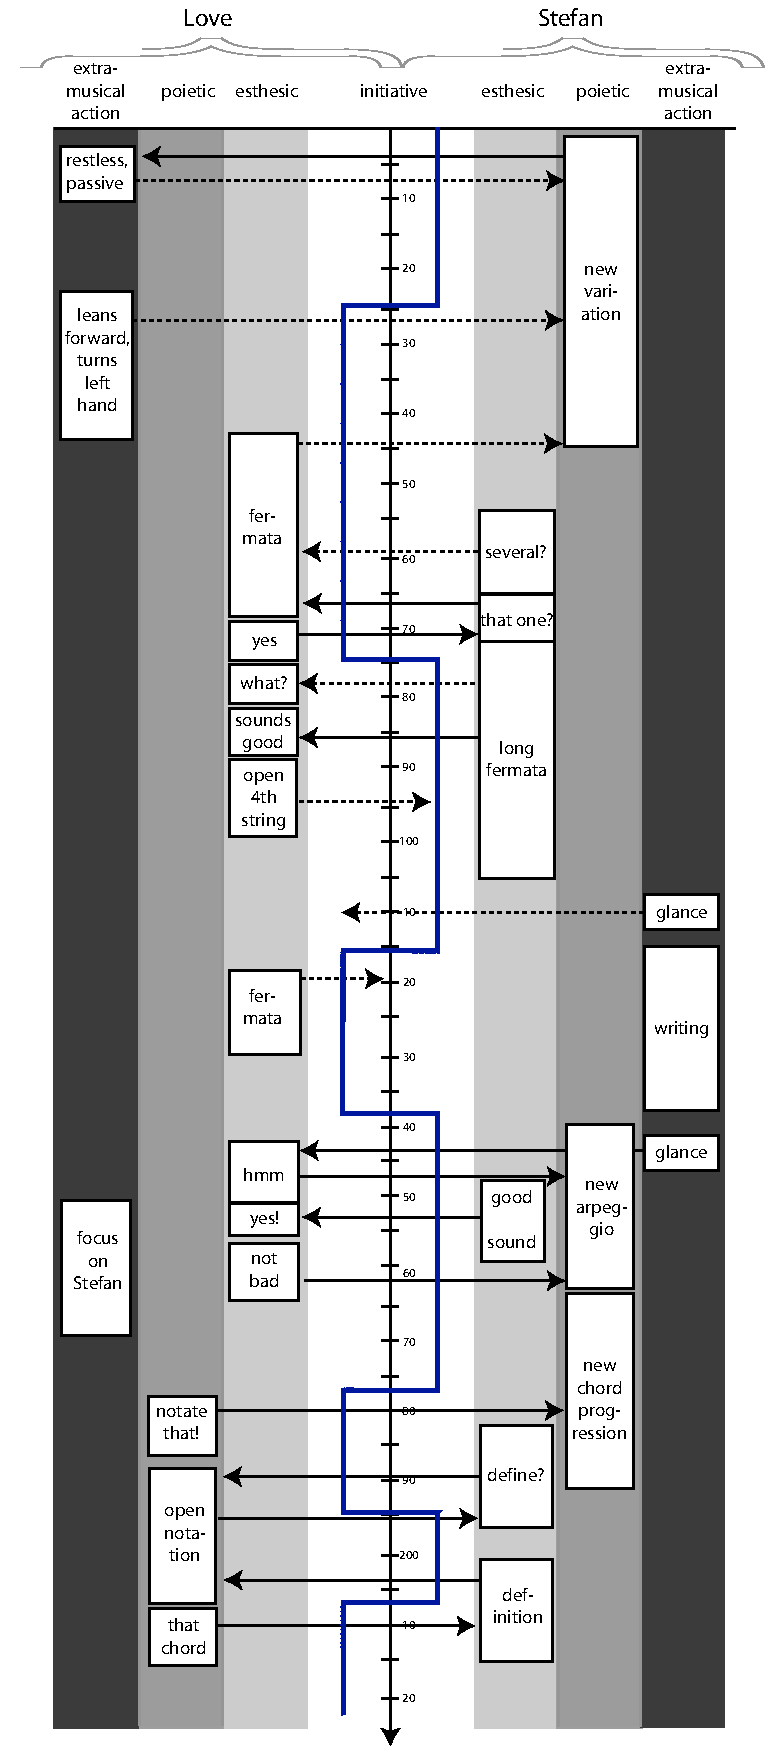
\includegraphics[height=0.85\textheight]{img/timeline_horiz}
    \end{center}
    \caption[A graph of the interaction between Stefan \"{O}stersj\"{o} and Love Mangs.]{A graph of the interaction between Stefan \"{O}stersj\"{o} and Love Mangs in the session analysed and discussed in Section \ref{sec:1-par:3}. The scale in the centre axis refers to line numbers in the transcription of the video and does \emph{not} represent linear time.}
    \label{fig:timeline-mangs}
   \end{figure}
% \end{wrapfigure}


\section{The Six Tones}
\label{sec:negotiating-2}

% \begin{wrapfigure}{r}{0.4\linewidth}
%   \begin{minipage}[h]{\linewidth}
%     \musicannot{The Six Tones\\\emph{for Dan Bau, Dan Tranh, % 10-stringed guitar, banjo and computer}\\Composed \& premiered in % 1996}
%   \end{minipage}
% \end{wrapfigure}
Another factor to consider while tapping into this process---the
process of constructing \emph{Repetition}---is the connection between \emph{Repetition} and a similar, but slightly larger, collaboration performed within the project \emph{The Six Tones}\footnote{As was explained above, the group \emph{The Six Tones} takes its name from the composition of the same name.} whose coming into existence is very closely related to \emph{Repetition}.
%%
%\marginpar{\listoftags{\tagword{Collaboration}, \tagword{Repetition}, %\tagword{Laptop}}}
%%
\emph{The Six Tones} was initiated in the spring of 2006, at a time when only sketches for \emph{Repetition} existed, when we had the opportunity to meet with two Vietnamese master musicians temporarily visiting Malm\"{o}: Ngo Tra My and Ngyen Thanh Thuy, playing the Dan Bau and the Dan Tranh respectively. Both are traditional Vietnamese string instruments, the Dan Bau an amplified mono-chord and the Dan Tranh a zither-like instrument. On a few occasions in May 2006 we met and improvised from a few loose sketches I had brought, Stefan on the ten-stringed guitar and the banjo along with Thuy, My and me on laptop. The intention was for these sessions to provide material for a new piece that I would compose.

\label{sec:2-par:2}
Though there are a number of interesting, but also problematic,\footnote{To mention only one aspect, Simon Emmerson has written about the difficulties involved in cross-cultural musical interactions and discusses the effect of \emph{masking} : ``Throw two traditions of music making together and aspects of one may \emph{mask} aspects of the other (sound subtlety, performance practice tradition and aesthetic intent)''. \cite{emmerson06}.} aspects to the project \emph{The Six Tones}---which I personally feel has become a very successful one---my primary concern here is not to discuss the project itself, but rather focus on its influence on my relation to composition. This discussion involves the significance of concepts such as `collaboration' and, more specifically, `interaction', as factors in the process of composition. In the previous \hyperref[sec:negotiating-1]{section (\ref*{sec:negotiating-1})}, we saw that, in a composer-performer collaboration the performer was not solely active in the \useGlosentry{glos:esthesic}{esthesic} domain any more than the composer was active only in the \useGlosentry{glos:poietic}{poietic} domain. This is however not the same as saying that this is a `natural' division of labour or an accepted form for work production.

\hypertarget{sec:target:negotiating-2-1}{It was suggested} \hyperref[sec:negotiating-1]{above} that Love Mangs was not entirely comfortable with the distributed nature of his role as composer in his collaboration with Stefan.\footnote{It should be mentioned that I have not discussed this with Mangs. My judgement here is based solely on how he acted in the video documentation of the collaboration.} There is a number of reasons why the idea of giving up part of that which is traditionally seen as the (sole) responsibility of the composer may appear provocative or of little concern to performers as well as composers. One is the classical (and obvious?) notions of power assigned to the `originator' as the authority on his (because it generally is a male) work: ``The \emph{explanation} of a work is always sought in the man or woman who produced it. [\ldots] the sway of the author remains powerful''.\footcite[143]{barthes68} Derek Bailey points to how Cannetti likened the conductor, ``the composer's proxy'', to a ``chief of police''.\footcite[Elias Canetti, \emph{Crowds and Power}. Citations from][20]{bailey92} Bruce Ellis Benson, in the last chapter of his book \citetitle{benson03}, points to the Kantian notion of the artistic genius as ``the epitome of the lone individual who wants nothing less than to speak in such a way as to supplant all other voices''.\footcite[164]{benson03} Nurtured by the idea of music as an autonomous art, the assumption ``that music making is primarily about creation and preservation of musical works''\footcite{benson03} also constructs our understanding of the composer and the composer's understanding of him or herself. The belief in and adherence to the autonomy of musical creation and artistic freedom makes it socially difficult for composers to give up their `power'\footnote{The concept of power with relation to New Music composers must be understood as relative to the field of music. As a genre New Music has suffered from extreme marginalisation in society, a phenomenon  referred to as the ``negative commodity value'' of music by Milton \citeauthor{babbitt58} in his infamous 1958 article: \cite{babbitt58}.}, as this could be interpreted as kowtowing to `the public' or trying to accommodate someone else's values, presumptively, according to the critic, in order to gain popularity. 

Whereas the \emph{author} had been killed already by 1968 because, according to Barthes, ``the birth of the reader must be at the cost of the death of the Author'',\footcite[148]{barthes68} the image of the `composer' as \emph{the} creator has resisted many attempts on its life.\footnote{Susan \citeauthor{mcclary89}'s essay \citetitle{mcclary89} in which the autonomy of the composer is questioned. The debate that followed (see \emph{Perspectives of New Music} 1992 and 1994) is indicative of the persistence of the Composer.\nocite{mcclary89}} Despite the developments of the last decades the socially and culturally, essentially romantic, idea of the composer is adherent: ``there is a special aura that envelopes composers, as well as other artists, because we think of them as true creators''.\footcite[Jerrold Levinson, \emph{What a Musical Work is} quoted in][37]{benson03} It is firmly rooted in the idea of the score, i.e. the notation, as \emph{the object} which is essentially preserved through the process of \emph{performance}: ``According to this model, composers create musical works and performers reproduce them''.\footcite[9]{benson03} But, as we saw in Stefan's collaboration with Love Mangs (see previous \hyperref[sec:negotiating-1]{section (Section \ref*{sec:negotiating-1})} and the associated \hyperref[fig:timeline-mangs]{Figure \ref*{fig:timeline-mangs}}) a composer's practice is not merely \emph{creation} (if we accept that musical \emph{creation} actually exists as a concept): equally important are the interpretative aspects. Even if the composing is not within the frame of a collaboration, the work of the composer may still be described as an interactive negotiation. Suppose a graph such as \hyperref[fig:timeline-mangs]{the one} drawn for the  Mangs-{\"O}stersj{\"o} collaboration was drawn for an imaginary project involving one sole composer working alone. If the composer's actions were plotted to the left, the right-hand side of the diagram, Stefan's side,  could easily be substituted by any one of a set of agents involved such as `guitar', or `skill', or something less tangible such as `musical style', and the resulting curve would probably be equally erratic. The point is that the composer, regardless of the presence of other humans, will always be in an ongoing interaction with different agents in the process of construction. 
% /Flytta

If the joint studies performed by Stefan and me described in \emph{Negotiating the Musical Work} \footcite{frisk-ost06,frisk-ost06-2}  (briefly summarised \hyperref[sec:negotiating-1]{above in Section \ref*{sec:negotiating-1}}) provided me with the theoretical insight that the internal negotiations I had always experienced while improvising as well as composing could in fact be brought out in the open, within the context of a collaboration, \emph{The Six Tones} gave me the chance to work these ideas out in practice. Now, obviously, despite the persistent view of the composer as ``the creator'', close
collaborations between composers and musicians as a method are not uncommon (at least not in contemporary music), nor are they new.\footcite[For a PhD dissertation devoted to the subject, see][]{ostersjo08} What is perhaps different here is how the processes engaged by \emph{The Six Tones} contributed to the development of \emph{Repetition}---a development that I had not foreseen. For my own reconstruction of my musical identity in this context---perhaps closer to musician than to composer (the (arbitrary) division between composer and musician will be examined in the next \hyperref[sec:negotiating-3]{section})---the May 2006 sessions with the Six Tones was important (see also \hyperref[fig:repetition-timeline]{the timeline in Figure \ref*{fig:repetition-timeline}}). Primarily because of the special circumstances that surrounded these sessions, I believe they influenced me in a way that made the transition towards \emph{openness} in the process of composition easier to commence and my receptiveness to this change was pivotal to the way \emph{Repetition} would develop from a `composition' into an open structure. The circumstances may be identified as impedance, as three modes of resistance, particularly in terms of \emph{The Six Tones}. In dealing with these resistances, in my attempts to overreach them, I had to address my habits and reappraise some aspects of the role of the composer. Although in reality these matters are not clear-cut, they may be summarised as:
\begin{enumerate}[(1)]
\item \emph{The language barrier}: Though Thuy speaks English, My understands and speaks it only a little, and English is not the first language of Stefan and me. In other words, even had I wanted to, I could not dictate how I intended the music to sound, at least not in verbal language.
\item \emph{The cultural barrier}: Unnecessarily cautious and afraid to fall into the trap of exploiting the cultural `Other', I proceeded very carefully, avoiding rigid instructions and   definitions.\footnote{Obviously instead falling into the trap of \emph{constructing} the `Other'.}
\item \emph{The musical barrier}: Prior to the project I had little knowledge of Vietnamese music. Considering how the currents of the cultural market flow, Thuy and My were likely to know much more about our music than we about theirs. How would we deal with musical `codes' and specific things like musical timing? These questions could only be successfully resolved in a meeting.
\end{enumerate}

%\begin{wrapfigure}{r}{0.65\linewidth}
\begin{figure}[!htb]
  \begin{center}
    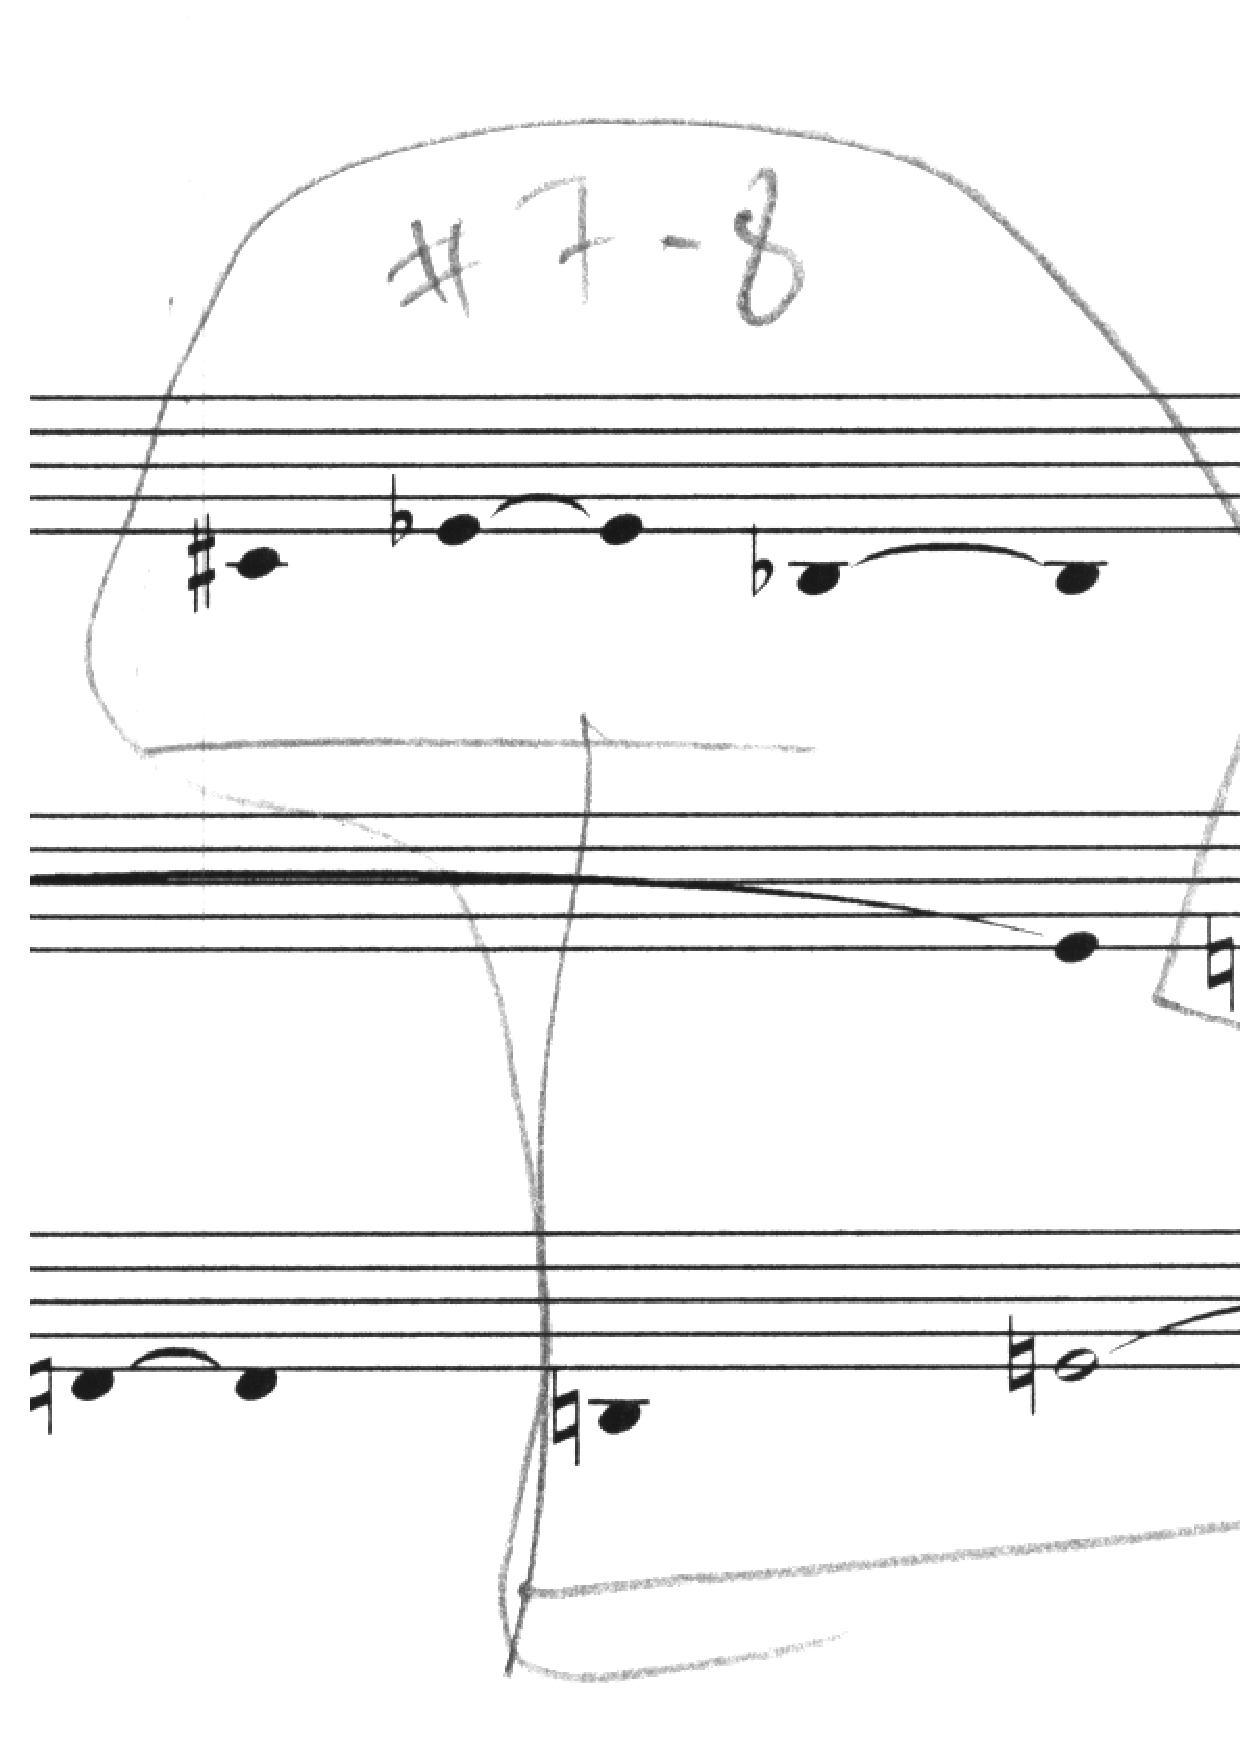
\includegraphics[width=0.75\linewidth]{img/SixTones-transcription-1}
  \end{center}
  \caption{The sketch used for the improvisations for the Six Tones}
\label{fig:sixtones-transcription}
\end{figure}
%\end{wrapfigure}

Apart from being artistically unsatisfying, writing a score to bring to these first meetings with the intention of having it performed `truthfully' would be futile. The chosen method, to improvise from sketches, gave us---all four of us---the opportunity to define our own \emph{subculture} (see \hyperref[sec:1-par:4]{section \ref*{sec:1-par:4}}) against which we could understand the possibilities and the limitations of our collaboration. For the formation of Stefan's and mine subculture, and for our collaboration at large, \emph{The Six Tones} had a great impact, particularly in the social dimension. Thanks to our project with Thuy and My, our process of `tuning-in' had an early start and thanks to it we were given additional opportunities to travel and work together. The importance of the social dimension should not be underestimated: When the construction of musical content is laid out in the open, mediated by a collaboration, the receptiveness of the social relation is paramount.

\emph{The Six Tones} was also important to \emph{Repetition} in the exchange of musical ideas between the two pieces. The sketches we used as a starting-point for our improvisations made use of the same material I had worked out for \emph{Repetition}, though, at the time the \emph{Repetition}-material consisted merely of a tone series in different permutations. For our session I had written out one of these permutations as a monophonic melody line laid out between the three string instruments as if it was one instrument playing (see \hyperref[fig:sixtones-transcription]{Figure~\ref*{fig:sixtones-transcription}}). A number of musical ideas from these sessions (altogether we met four times in May 2006) had a tremendous influence on how the ideas for \emph{Repetition} evolved and how the material was composed.
\begin{itemize}
\item Prior to the Six Tones sessions the idea was to write for six-stringed guitar but the register and the possibilities for alternative tunings persuaded Stefan and me to choose the ten-string guitar instead. 
\item One of the sections of \emph{Repetition} is a transcription of one of the improvisations on the sketch brought to the session on May 17.
\item The scordatura used in \emph{Repetition} was developed according to the   needs presented by the Six Tones project.
\item Some of the sound files used in the first version of \emph{Repetition}   used samples recorded during the Six Tones sessions. 
\end{itemize}  
But there was also a flow of ideas going the other way, from \emph{Repetition} to \emph{The Six Tones} as material composed for the guitar piece was transcribed and used in the ensemble piece.

\section{The first version}
\label{sec:negotiating-3}

\begin{wrapfigure}{r}{0.45\linewidth}
  \begin{minipage}[h]{\linewidth}
    \begin{flushright}
      \musicannot{Repetition Repeats all other Repetitions\\
        \emph{for ten-stringed guitar and computer}\\
        Composed \& premiered in 2006\\
        Commissioned by and dedicated to Stefan \"{O}stersj\"{o}}
    \end{flushright}
  \end{minipage}
\end{wrapfigure}

%%% Local Variables: 
%%% mode: latex
%%% TeX-master: "../ImprovisationComputersInteraction"
%%% End: 

With regard to the background for \emph{Repetition} yet another aspect should be mentioned: its intertextual relation with \emph{Toccata Orpheus} by German composer Rolf Riehm. I became acquainted with \emph{Toccata Orpheus} when Stefan and I participated in the workshop \emph{Knowledge Lab} in Berlin in June 2005. Stefan performed the piece (composed in 1990 for six-stringed guitar solo) and discussed its artistic and interpretative implications in the workshop. Following this event we repeatedly discussed Stefan's idea of making a multimedia performance of \emph{Toccata Orpheus}---i.e. a staging of the piece to allow for a broader expression and a shift of focus to the physicality of the piece. This performance version would involve a sound-scape by me and, during the process of discussing \emph{Toccata Orpheus} and a possible soundscape, we recorded the piece in its entirety as well as details of it for me to use as samples in the sound-scape. We also made a video recording of it that I edited and I started elaborating on the idea of using this material for an electro-acoustic piece with video, addition to the sound-scape. Though introverted in its expression, \emph{Toccata Orpheus} is a highly visual piece as the many different and unusual playing techniques have become part of its construction: there is as much to look at as there is to listen to. Hence, when I started working on the score for \emph{Repetition} in August 2006 the Riehm piece was most certainly a source of inspiration, because I had so closely studied it and discussed its possible performances with Stefan over a long period of time and because I was inspired by the dramaturgy involved in the performance of the piece. In \emph{Toccata Orpheus} the more radical and strained the movement required of the performer the lesser the sound---in itself an interesting reversal of force. In preparation for the sound-scape mentioned above I had made an analysis of the piece based on the movement required to perform each sound, and classified the phrases according to this analysis. The way I decided to approach \emph{Repetition} was very similar: I borrowed Stefan's ten-stringed guitar and constructed a set of sounds based on different playing techniques, some of which are part of contemporary guitar technique and some of which I invented.

\label{sec:3-par:2}
As mentioned above, the raw material for the piece was a simple tone series, a version of an infinitely self-repeating series common to much of Danish composer Per N{\o}rg{\aa}rd's music. Conceptually the piece consists of three permutations of the same raw material, labelled \emph{A}, \emph{B} and \emph{C}. These three motives, distinct both sonically and expressively, are, in a manner of speaking, telling the same story in three different ways. Though it is only possible for the guitarist to play one of these motives at a time, irregularly moving back and forth between them, with the help of the computer part---also made up of three corresponding materials---she or he could create the illusion that all three `stories' are told simultaneously. The guitar and the computer merely `give light' or resonate with one version of the story at a time. The intention was to let the order of the fragments belonging to the three motives be the result of decisions made in performance. In other words, the score consisted of a collection of composed fragments pertaining to one of the three motives and it would be up to the performer to choose the order and the number of repetitions each fragment would play. The interactive challenge, i.e. the question of how to get the computer to `perform' with Stefan without the order, or form, of the music being known in advance, had been factored in already from the start of the our collaboration. \emph{Repetition} was thought to be a testbed for my analysis \index{software}software \emph{timbreMap}, which is a self organising feature map that when fully trained may automatically detect timbral differences in the input audio signal. The idea was to have the \index{software}software `listen' to Stefan and be able to detect when he moved from playing, say, a fragment of the \emph{A} material to some \emph{B} or \emph{C} material. For this reason too it was necessary for me to compose the three materials in such a way that they would be sufficiently timbrally distinct from each other for the \index{software}software to detect the change. At this time, in August 2006, I had a proof-of-concept version of \emph{timbreMap} working which gave me a chance to evaluate and test the different playing styles and their effect on the `listening' computer.

\label{sec:3-par:3}
Though the technique, i.e. the \emph{timbreMap} \index{software}software as interface, may well have worked for the first performances in 2006, we soon realised that for practical reasons with a paper score it would be impossible to employ the level of freedom intended. The six-page score would have to be entirely visible throughout the piece for Stefan to be able to move freely from motive to motive and from fragment to fragment. Though it is possible to set the score up on six music stands it would not be possible to read it.\footnote{In classical guitar technique the guitarist is sitting down, and though in some music it might be possible for the guitarist to move around (most certainly in all other genres), the alternate playing techniques used in this piece make it impossible to play without sitting down.} The solution we chose was to move the decisions concerning the large-scale form of the piece to the pre-performance phase. Stefan would simply work out his version in \index{real-time}\index{time!real-time}non-real-time, and together, following Stefan's instructions, we made a performance version of the score. With time being short and the first performance quickly approaching we also decided to make the interaction between Stefan and the electronic part in this version governed by a foot pedal. Stefan could simply trigger sound-files stored on the computer by pressing a foot switch. This version is still interactive to a certain extent but it is so only if you do \emph{not} consider what the intention had been. How could the original intentions of the piece be `given up' so easily? Neither I nor Stefan saw this first version of \emph{Repetition} as anything other than one possible `version' out of many to come. This agreement was the first step towards the notion of a `\useGlosentry{glos:work_in_movement}{work-in-movement}'\footnote{The term `work-in-movement' was coined by Umberto Eco to distinguish a particular species of `open works' in which ``the auditor is required to do some of this organizing and structuring of the musical discourse. He collaborates with the composer in making the composition''. In the case of \emph{Repetition} the `auditor' is replaced by the performer but that is also the case in the examples of work-in-movements that Eco provides. \cite{eco68}.} and by limiting the openness in this particular instance we greatly increased the future possibility for openness. This expanded concept of openness or work-in-movement---whereby each instance could not only choose its form in the course of the performance, but alter its interaction scheme, its instrumentation, its score, and so forth---was not originally specified by me. If Peter Kivy is right in suggesting that \emph{discovery} is what best describes the activity of composers,\footcite[214]{kivy02} then we were truly composing when we impeded \index{real-time}\index{time!real-time}real-time choice in the first version of \emph{Repetition} because, in this and other choices we made, its potential as a `work-in-movement' was \emph{discovered}.

%%
%\hspace{0.5\linewidth}
\begin{wrapfigure}{r}{0.5\linewidth}
  \begin{minipage}[H]{1\linewidth}
    \advance\rightskip-1cm
     \vspace{0.5cm}\label{fig:inlay2}
\musicannot{
Marcel Duchamp, introduced the notion of the ``personal 'art coefficient' '' in a discussion concerning the creative act. Specifically Duchamp was referring to the immanent processes, those in which the artist alone is involved and which ultimately lead to ``art in the raw state---\`{a} l'\'{e}tat brut'' and, in short, it constitutes the difference between the artistic intention and its realization. The gap goes unnoticed by the artist and it represents his (or her) inability ``to express fully his intention''\footcite{duchamps57} Duchamp concludes that ``the personal 'art coefficient' is like an arithmetical relation between the unexpressed but intended and the unintentionally expressed.''\footcite{duchamps57} It is primarily the description of the art coefficient as a \emph{relation} that I find interesting. What could the `interaction coefficient' constitute? The notion of the ``unintentionally expressed'' as having a relation to the ``unexpressed but intended'' could be directly transferred to interaction: In any interaction there are unintended outcomes (\emph{Why did the computer go down?} or \emph{Why did you sound so angry?}) as well as intended but tacit (\emph{How come the computer doesn't understand what I want to do?}). What can the interaction coefficient tell us about an interaction? What, if the interaction is part of an artistic context, what would the relation between the art coefficient and the interaction coefficient be? Would they be the same or different?
}
  \end{minipage}
\end{wrapfigure}
%%% Local Variables: 
%%% mode: latex
%%% TeX-master: "../ImprovisationComputersInteraction"
%%% End: 

%%
\label{sec:3-par:4}
Another reason we allowed ourselves to change the scheme of the piece, and to continue to do so, was the fact that in the rehearsals it was obvious the alterations had worked out really well. Not only was the new form convincing, the integration between the electronics and the guitar was seamless. Despite the lack of performer-computer interactivity, several listeners in the audience for the first performances commented that the piece sounded like it was interactive (i.e. interactive in the sense I had intended it to be). Some even thought it was and were surprised to learn about its relatively static set-up. The sounds I used for the electronic part were samples from the improvisations we did with \emph{The Six Tones} (see \hyperref[sec:negotiating-2]{Section~\ref{sec:negotiating-2}}) as well as samples I had from playing Stefan's ten-stringed guitar when composing the score for \emph{Repetition}. Could it be that the interaction in the production phase of \emph{Repetition} substituted for the \index{real-time}\index{time!real-time}real-time interaction in the performance? This would imply that interactivity is a quality that `objects' can absorb or occupy, that they can pick up and then adhere to, independent of time. The interaction between Stefan and me, and between us and Thuy and My (in the project \emph{\useGlosentry{glos:six-tones}{The Six Tones}}), was encoded in the sound-files used for the computer part and in the music as performed. Certainly a pleasing thought, though I doubt the reason for the deceptive impression of performer-computer interactivity in this version of \emph{Repetition} is directly related to interaction of a different kind and in a different time (although interactivity does not necessarily have to be \index{real-time}\index{time!real-time}real-time as discussed in \hyperref[sec:time-interaction]{Section \ref*{sec:time-interaction}}) but I believe that, in musical practice, interaction of the kind Stefan and I were engaged in whilst preparing for these first performances is a factor (a coefficient?) that positively influences the chances for a successful result---where `successful' is defined as `all participants are generally pleased with the outcome'. It is this coefficient that creates the illusion of performer-\index{interaction!computer}computer interaction.


\section{Symphonie Diagonale}
\label{sec:negotiating-4}

\begin{wrapfigure}{r}{0.5\linewidth}
  \begin{minipage}[h]{\linewidth}
    \begin{flushright}
      \musicannot{
        Repetition Repeats all other Repetitions, Symphonie Diagonale\\
        \emph{for ten-stringed guitar, computer and video projection}\\
        Composed \& premiered in 2007\\
        Prepared in collaboration with Stefan \"{O}stersj\"{o}}
    \end{flushright}
  \end{minipage}
\end{wrapfigure}

%%% Local Variables: 
%%% mode: latex
%%% TeX-master: "../ImprovisationComputersInteraction"
%%% End: 

The  motivation for the second version we did, the combination of \emph{Repetition} and \emph{Symphonie Diagonale},\footnote{The silent movie \emph{Symphonie Diagonale} is an eigth-minute modernist film classic by the Swedish artist Viking Eggeling dating from 1924.} was to use the film as a springboard for the making of a radically different version of the guitar and electronics piece. By itself, the idea of combining two totally unrelated works, separated in time by 83 years and created in different media, is extremely odd but the first version of \emph{Repetition} had already been performed four times and it was at this point scheduled for another four performances. Though the potential for \emph{Repetition} as a work-in-movement had been discovered, its status as such had not yet been established and, owing to the `success' of the first version, we had to resist the comfortable notion of staying with the first version. Hence there was a need for a second version as different from the previous one as possible. 

\label{sec:4-par:2}
This version is even less interactive than the first in that its performance version is static: the film, along with the electronic track, is played back and Stefan is solely responsible for keeping the synchronisation tight between the film and the electronics on the one hand, and the guitar part on the other. The binary control interface is now reduced to constitute zero or one: the video is either playing or it is not. Again, we have to see the bigger picture and look at the processes that proceeded the performances of the second version.\footnote{The process of constructing this version is described in some detail in \cite{ostersjo08}.}

\begin{wrapfigure}{l}{0.2\linewidth}
  \begin{center}
    
\includegraphics{img/eggeling-25}
  \end{center}
    \caption{Symphonie Diagonale}
    \label{fig:eggeling-25}
 \end{wrapfigure}
\label{sec:4-par:3}
If for the first version there was a relatively clear distinction between my tasks (providing the raw material, the score and the sounds) and Stefan's (constructing a performable version of the piece out of the components I gave him), our interactions for this version were less defined. After an initial analysis of the film, an obviously black and white eight-minute abstract film---white graphical shapes, evocative of paper cut-outs, on black background (see \hyperref[fig:eggeling-25]{Figure \ref*{fig:eggeling-25}})---we started mapping the musical material onto the imagery. We were working with a recording of the guitar part, and many of the phrases fitted the rhythm of the film without alteration: we were inspired by the lack of resistance of the undertaking and the version was completed in a few days. 

\label{sec:4-par:4}
The work we did on those days in January 2007 involved a great many artistic choices that were all made by continuous negotiation between `performer' and `composer' with an almost complete merging of the two agents into one \emph{musician}. Neither of the agents seemed to have the interpretative precedence and, to use the terminology from \autoref{sec:1-par:3}, the \emph{\useGlosentry{glos:poietic}{poietic}} and \emph{\useGlosentry{glos:esthesic}{esthesic}} domains overlap and interact in a recursive fashion. Again, the interactivity in the performance WAS supplemented by interactivity in the construction. Although, as I pointed out above, the main purpose of this version was to create a breach that would allow us to move on to yet another version of \emph{Repetition}, the film component added an extra constraint: if we wanted to stay faithful to the film, i.e. not alter it in any significant way, then the non-interactive, static rather than dynamic version we ended up with was almost our only option. Why then did we not alter the film? It is perfectly possible to take \emph{Symphonie Diagonale} and cut it up into small fragments that get triggered by the guitar or by the audience or by any other factor. In the making of this version, the film was the method, rather than the result, the intended result of which was to further open up the work \emph{Repetition}. In that sense this version was an intermediary between the first version and any succeeding ones.

\label{sec:4-par:5}
At this point, after the \emph{Symphonie Diagonale} version had been performed it started to become clear that \emph{Repetition} had in it an infinite number of \emph{Repetitions}. Its `authenticity' lies in the collaborative aspects of its production `versioning'\footnote{\index{software}Software versioning, also known as revision control, is used to differentiate between different editions or `releases' of e.g. software.} rather than its detailed specifications. Its material work identifying instructions---in this case the scores, the samples and sound-files, the recordings of prior performances; everything belonging to its prior versions---could be picked up by any two or more musicians willing to engage in the construction of another version (in the sense of construct rather than construe).

\section{Collaborative music}
\label{sec:negotiating-5}
Collaborative artistic work in general may be seen as a reaction against the singularity of the romantic as well as modernist view of the artist as the inspired, predominantly white male creator from whom great artworks emanate. It is, however, very difficult to draw a distinction between collaborative work as decentralised division of labour on the one hand and, let us call it, less collaborative work that stems from centralised authority on the other. To begin with, in music, it is difficult to imagine a performance that does not involve collaboration between different agencies at some level of the production. Perhaps the \emph{Study No. 21, Canon X}\footnote{Studies No. 4 through 30 were composed between 1948 and 1960.} from \emph{Studies for Player Piano} by American composer Conlon Nancarrow can serve as an example of `less-collaborative' music. Not only was it composed for a mechanical instrument\footnote{Like so much of Nancarrow's other music, \emph{Study No. 21} is written for a player piano, the Ampico player piano to be specific (see \url{http://en.wikipedia.org/wiki/Player_piano} for more information on these instruments).} and punched into the player roll rather than written out in traditional notation, it was not performed in public (with one exception) until after Nancarrow's international breakthrough in 1982. The following is an excerpt from an interview with Nancarrow by William Duckworth that gives evidence of the seclusion and non-collaborative environment in which this and the other Studies were composed:
\begin{squote}
  \emph{Duckworth}: Between the early 1940s and 1960, when you were writing most of your Studies, was anyone hearing your music besides you?\\
  \emph{Nancarrow}: No.\\
  \emph{Duckworth}: Were you just playing them for yourself?\\
  \emph{Nancarrow}: Occasionally someone would hear it, but very
  occasionally. \footcite[49]{duckworth99}
\end{squote}

\label{sec:5-par:2}
At the other end of the collaborative/non-collaborative continuum, we could place any example of free jazz group improvisation in which nothing is pre-determined apart from the instruments, the players and the physical (and usually social) context. Evan Parker writes about a recording of a trio improvisation featuring, apart from himself on saxophone, Derek Bailey and Han Bennink: ``We operate without rules (pre-composed material) or well-defined codes of behavior (fixed tempi, tonalities, serial structures, etc.) and yet are able to distinguish success from failure''.\footcite[As cited in][39]{lebaron02} A lack or dismissal of ``rules'' of operation or ``codes of behavior'' is not necessarily a prerequisite for collaboration but may be seen as a method by which the participants are forced to collaborate in order to avoid cacophony and chaos. (Though, admittedly, chaos may also be a most viable means of collaborative expression.) 

\label{sec:5-par:3}
A different beam of collaborative music (forced collaboration?), orthogonal to the Nancarrow-Parker axis, can be found in the brilliant and skilful output of John Oswald, who coined the term `Plunderphonics' for a ``retro-fitted music, where collective melodic memories of the familiar are minced and rehabilitated to a new life''.\footcite[Oswald quoted in][49]{lebaron02} By cutting up recordings of popular music into small chunks and pasting them together in unexpected combinations he created a schizophrenic music---perhaps the very epitome of postmodern music---in which seemingly random collections of snippets of sound are forced to collaborate.\footnote{Recommended listening is the 1'46'' long \emph{Cyfer} on the CD \emph{Plexure}: \cite{plexure93}} Although the artists whose music he reorganised rarely agreed to the refactoring,\footnote{Based on Michael Jackson's song ``Bad'' Oswald's collage ``DAB'' from the 1995 CD \emph{Plunderphonics} caused a copyright debate with legal consequences more than a decade before peer-to-peer sharing and illegal downloading. CBS Records, Michael Jackson and the Canadian Recording Industry Association claimed that Oswald's work was illegal and demanded that the recordings of his work be destroyed. \cite[See][]{wired95}.} Oswald, in a manner of speaking, set up a distant collaboration with them and with the context they belonged to, comparable to Marcel Duchamp's readymades. On the opposite side to Oswald, but on the same axis, we could place any kind of \useGlosentry{glos:fixed_media}{fixed media}, electro-acoustic so-called `tape piece' (i.e. studio produced music played back in concert on speakers), such as John Chowning's \emph{Stria}, in which all sound material used is synthesised (as opposed to sampled real-world sounds.

\label{sec:5-par:4}
These are examples of regions of musical collaboration in a multiaxial space of musical practice. As mentioned above, some degree of collaboration is likely to play a part in any music and, as a consequence, it may be suggested that `collaborative', when used to describe the coming into existence of a musical work, is too unspecific. If so, how may the multiple, collaborative, \useGlosentry{glos:poietic}{poietic} processes of \emph{Repetition} be described? That `work-in-movement' may be used to define the work type it belongs to is of little help; it only tells us that we are dealing with an unfixed work and that it needs involvement of others apart from the composer to be instantiated, but not what the nature of the collaboration constitutes. Depending on the version we are examining, \emph{Repetition} as a `work-in-movement' will inevitably move between many different locations in the collaborative space proposed above. Looking back at the phase at which the work revealed its possibilities for openness (\hyperref[sec:4-par:5]{see the last paragraph of \ref{sec:negotiating-4}}) we may conclude that collaboration constitutes the ontological essence of the work: it is a work whose identity is to be found in the interactions that has preceded its productions rather than in its instructions. The collaborative aspect of \emph{Repetition} is the work.


% Although most musical activities involve collaboration of some kind, in \emph{Repetition} collaboration is the very essence of the work.

% the particular kind of collaboration that evolved while working on \emph{Repetition} may be distinguished in that it constitutes the very essence of the work.

%  it is perhaps possible to distinguish the kind of collaboration identified with \emph{Repetition} from the range of collaborative activities that make part of most musical activity in that the collaborative aspect in \emph{Repetition} has been made its essence.

%%%%%%%%%%%%%%%%%%%%%%%%%%%%%%%%%%%%%%%%%%%%%%%%%%%%%%%%%%%%%%%%%%%%%%%%%%%%%%%%
\section{The annotated score}
\label{sec:negotiating-6}
%%%%%%%%%%%%%%%%%%%%%%%%%%%%%%%%%%%%%%%%%%%%%%%%%%%%%%%%%%%%%%%%%%%%%%%%%%%%%%%%

\emph{Repetition} was conceived prior to its preparatory studies and the experiences gained from its first and second versions as an open work similar to some of my other works like \hyperref[sec:drive-2003]{\emph{Drive}}. It was manifested as building blocks notated and left to the performer to organise them: a fairly traditional example of `open work'. The way the process has evolved, however, informed by the knowledge produced in the study performed on Stefan and Love Mangs (\hyperref[sec:negotiating-1]{see Section \ref*{sec:negotiating-1}} and \ref*{sec:negot-music-work}), the emphasis in the term `work-in-movement' has travelled from `work' to `movement', and the emphasis on the `composer' in the quote from Eco\footnote{``The auditor is required to do some of this organizing and structuring of the musical discourse. He collaborates with the composer in making the
composition.'' \cite{eco68} The auditor is interchangeable but not the composer.} should in our case instead be put on `collaborate', because the action is more important than the subject. Altogether, we have  travelled quite a long way from Eco's original notion which, to begin with, by the `auditor' implies a (passive) `receiver' rather than a collaborator. The `work-in-movement'  implied here is a literal construction kit, to be assembled and re-assembled in a recursive process that should be allowed to continue outside the collaboration that gave rise to it. Stefan and I set it in motion but its authenticity can only be derived from the continuous movement, an open-source music that may be dismantled and reconstructed, added to and altered, according to its conglomerate of participants.

In order to realise fully the notion of a work-in-movement, the process of documentation, or in musical notation terminology the work identifying instructions, needs to be reconsidered. The way \emph{Repetition} as a work has evolved, a traditional printed score in musical notation, no matter how detailed the written instructions are, would be misleading. As has already been pointed out, the operative word in `work-in-movement' is precisely the movement: the change, the difference that makes a difference. Therefore the score will need to communicate the process rather than the result, in itself not a novel idea. The musical notation will no doubt constitute an important part of the documentation but it will not be sufficient in itself.

As discussed, apart from this more, let us call it musicological, aspect of the notation of \emph{Repetition}, there are also practical issues regarding the notation and the score that need to be resolved in order to allow for the work to continue to evolve. If the performer is to be able to alter the order of the sections according to choices made in performance, the score needs to be adopted. If, however, the performer chooses to do what Stefan did in the first version, i.e. settle on a form prior to performance, the `final' score should easily allow for this. Finally, adding the third version discussed above---with a real-time interactive computer part---to the list of possible modes of performance, the score needs to fully document and guide the performer in how to set up the computer part. 
\begin{figure}[htb]
  \centering
  \includegraphics[width=\linewidth]{img/Work.png}
  \caption[The IntegraBrowser: base record.]{The IntegraBrowser displaying the base record for \emph{Repetition Repeats all other Repetitions}.}
  \label{fig:ib-1}
\end{figure}

\begin{wrapfigure}{r}{0.4\linewidth}
  \begin{minipage}[h]{\linewidth}
    \begin{flushright}
      \musicannot{IntegraBrowser\\
        \emph{Offline browser for the Integra XML\\documentation format.}}
    \end{flushright}
  \end{minipage}
\end{wrapfigure}

%%% Local Variables: 
%%% mode: latex
%%% TeX-master: "../ImprovisationComputersInteraction"
%%% End: 

To allow for these considerations---the performance aspect and the `work-in-movement' aspect---I have developed an experimental web application\footnote{A Web application is a piece of software that is run in a standard web browser.}. This application is an attempt at allowing for what may be termed the `annotated score', an information source relating to a piece of music (or any other kind of art work) that may hold a score and any number of other documents referring to the piece (an audio or video recording, a performance instruction, text instruction, information on previous `instances', etc., all of which may be interlinked). With the Web application, called the Integra Browser, such collections of heterogeneous data pertaining to \emph{Repetition}, or any other piece of music or general art work, may be browsed and edited (see the screenshots provided in Figure \ref{fig:ib-1}, \ref{fig:ib-2} and \ref{fig:ib-3}). The design considerations set up for the annotated score were that
\begin{itemize}
\item It should encourage the interpreter to engage in a collaborative
  process similar to the one we have gone through with the primary
  goal of not repeating or recreateing our process but to find his or her
  own unique version.  
\item It should allow the performer to look up any part of the
  notation at any time.
\item It should allow for the interpreter to easily create a static
  form that s/he can use in performance.
\item It should contain all the \index{software}software and all the sound-files needed
  to create an interactive as well as a non-interactive version of the
  computer part.
\item It should document important parts of our collaboration and
  allow for other performers to add important parts of their own
  collaborations to the work.
\end{itemize}
Realising the first versions of the notion of an annotated score and fulfilling these design goals is possible by making use of the \emph{libIntegra} framework and the associated IXD file format.\footnote{The details of the format is described in \cite{frisk-bull07}. See also \cite{frisk-bullock08}}

\begin{figure}[htb]
  \centering
  \includegraphics[width=\linewidth]{img/Score.png}
  \caption[The IntegraBrowser: an instruction video.]{A second pane displaying a score snippet with an associated instruction video.}
  \label{fig:ib-2}
\end{figure}

\begin{figure}[htb]
  \centering
  \includegraphics[width=\linewidth]{img/Discourse.png}
  \caption[The IntegraBrowser: meta-information.]{This panel shows how meta-information and different modes of analysis may be attached to a score. This picture is mapping the interactions between the different agents in my collaboration with Stefan \"{O}stersj\"{o}.}
\label{fig:ib-3}  
\end{figure}

\section{Summary}
\label{sec:summary-2}

In this chapter I have tried to unwrap the process that led to the work-in-movement \emph{Repetition Repeats all other Repetitions} and the significance of the pre-study phase in which Stefan and I attempted a closer understanding of the musical collaboration as method. These studies provided important information that shaped how the project evolved. \useGlosentry{glos:six-tones}{The Six Tones} (working on the piece as well as working with the group) and the experiences gained from working with Vietnamese music in general further deepened the collaborative aspect of the project which neither one of us had yet fully conceived of as the open work type that had begun to emerge. The first performance version deviated from almost all aspects of the intention of the piece and for the same reason provided us with an opening towards a different understanding of open form. Therefore, the collaboration did not end with the first performance, rather, it had just started. The need to break loose from that version gave birth to the idea of a version for the abstract dadaist film \citetitle{eggeling24} by \citeauthor{eggeling24}. Again, this version took us further away from the original intentions but closer to the new intention: the concept of the work-in-movement. A short overview of music and collaboration, and some possible points along the collaborative/non-collaborative continuum were presented. Finally, the augmented score as a carrier of a work-in-motion was proposed. An experimental version of a Browser for augmented scores built on top of the Integra framework and file format was presented. 

It is my hope that \emph{Repetition} will not come to a halt but continue to develop. Versions for other (string) instruments are possible, but also versions for computer(s) only. A work-in-movement thrives on its motion and must not stagnate.
\newpage
\thispagestyle{empty}
%%% Local Variables: 
%%% mode: latex
%%% TeX-master: "../ImprovisationComputersInteraction"
%%% End: 

\chapter[Interaction]{Interaction and the Self}
\label{sec:interraction-self}
In the following text I discuss the concept of interaction and its relation to different technologies, the meaning of the different kinds of interaction and (musical) examples of their usage. As with some of the other texts I combine several different modes of reflection in what may best be described as a non-structured manner although it should be clear that the reasons for this organizations are more closely related to method than to lack of method. It is my hope that the reader, in spite of the non-structure, will be able (and willing) to navigate through these thoughts.

Since I first started using computers in my musical practice in 1994 I have been searching for ways in which to use them creatively while improvising as well as composing. In most of my compositions since then the \index{computer}computer is incorporated as a `player' along with acoustic instruments and in recent years I have also begun to perform \emph{on} the computer, as opposed to playing it through another (acoustic) instrument. In the beginning, however, my dominant interest lay in improvising with the computer, in playing saxophone and using that which I played to give the computer the impulse to play with me. Interacting with a computer in the context of (improvised) music raises inevitable questions regarding the interaction, its prerequisites and its needs, and it is not obvious how to pose the questions. The questions may look at the matter from the `outside'---e.g. analysing and evaluating that which I do or try to do, leaning towards established theories---and they may investigate the `object' from the `inside' by turning to the actual \emph{playing}. In this project I use both methods, which obviously have to overlap to a considerable degree. The questions will not always be the same but will vary with context and with time, just as the needs imposed on the interaction will not be the same for every situation. This research project is about raising issues that allow me and others to keep asking and reformulating these questions as new technology becomes available and new knowledge is produced. The somewhat ambiguous genre identifier \emph{interactive computer music} (is there a music which is \emph{not} interactive in some sense?) may easily encompass all of the contexts in which I am and have been active, as well as many others, depicting a music in which computers or other electronic devices or instruments are manipulated in \index{real-time}\index{time!real-time}real-time. The discussion below is an attempt to untangle the meaning and significance of \emph{interactive} and \emph{\index{real-time}\index{time!real-time}real-time} with regard to my own artistic practice and aesthetics.

The first years of playing, in every sense of the word, with the computer, despite the laptop's immaturity and the fact that any `direct manipulation' of audio was out of the question, were very creatively stimulating for me. But, after the initial fascination with the ostensibly interminable possibilities of the computer as `instrument' had worn off, several issues were called into question. What is interaction? What does it mean to interact with a computer? Should the interaction with the computer be different from interacting with a fellow \useGlosentry{glos:musician}{musician}? Is there any reason at all to `play' with a computer (rather than with a fellow musician)? Do I want to play `with' or `on' the computer? When I play, what do I express that has bearing on the current musical expression and, if successfully extracted, can that information be quantified and transformed into meaningful, machine-readable data? This last question may be said to summarise, albeit very briefly, one of the challenges of interactive \index{electro-acoustic music}electro-acoustic music: to develop \emph{interfaces} that may act as intermediaries between performer(s) and computer(s).\footnote{Gestural control, where ``gesture is used in a broad sense to mean any human action used to generate sounds'' \parencite[E. R. Miranda and M. M. Wanderley as quoted in][39]{jensenius08} is a large and very active field of research, which in a sense may be said to be closely related to (traditional) instrument design. The yearly NIME conference (see \url{http://www.nime.org/}) is devoted to the topic and \citeauthor{jensenius08}'s PhD dissertation referenced above discusses gestural control in (electro-acoustic) music. For a general overview of ``interface typologies'', see \cite[135-42]{emmerson07}.} In a situation with one \useGlosentry{glos:musician}{musician} and one computer involved in an interactive performance, \emph{if} it is of interest that the sounds produced `blend', that they may be perceived as having some attribute in common, though this attribute may not necessarily be known or even identifiable, what are the necessary prerequisites that would allow the sounds to `blend'? How can a `common ground', some sensation of unity, or ``\emph{fused sounds}'',\footcite[126]{emmerson07} be established between the actual and the virtual performer and how are the relevant parameters communicated between the different players? These were essentially the questions that led me into this project and, though still highly relevant, the issues of \emph{what} and \emph{how} to communicate with the machine have become subordinate to the question of the interaction itself. By that, I mean to say that a clouded concept of the intentions and purposes of the interaction, of the particular contextual meaning of interaction, is likely to result in an equally clouded interactive system. 

The subject of `blending'---perhaps a more appropriate term is `sonic interaction'---was briefly discussed in the \hyperref[sec:introduction]{Introduction} in the \hyperref[sec:timbremap]{section on \emph{timbreMap}} and the remainder of this section will deal with questions pertaining to the topic of musician-\index{interaction!computer}computer interaction. The question `What is interaction?' is clearly not specific to the field of music. Or, to put it more precisely and less axiomatically, though it is not particular to music, the way interaction is dealt with in the field of music is to a large extent informed by how it is dealt with in other realms, such as the social or the technological. \hypertarget{sec:target:interraction-self-1}{Inversely, any findings} within the field of music made with regard to interaction \emph{may} have general relevance, but may just as well be specific to music, interactive music, or even only the particular case. In other words, as with many concepts there is a terminological fluidity involved which necessitates a discussion involving several aspects of the subject matter. Below, I attempt such an undertaking, also using experiences of interaction accumulated from \emph{Drive}, \emph{etherSound}, \emph{timbreMap} and \emph{Repetition Repeats all other Repetitions}.

\section{Interactive Music}
\label{sec:interactive-music}

Before we discuss the implications of interaction independently of the field of music, the conception of interactive music itself, the focal point of this book, needs to be considered. Not only is the term by itself misleading and ambiguous, in practice, as a genre, it is used to denote so many different kinds of musical activities that the question of interaction loses its meaning.

What then is \emph{interactive music}? That question prompts a rhetorical defence. Is there a music that is not interactive? That does not interact with its environment and its listeners in some way? Depending on the context, commonly when the term \emph{interactive} is used, it is often implied that one of the `subjects' in the interaction is a computer or some other electronic device. This holds true also for music: interactive music implies computer music which is paradoxical because, if interactive music equates with interactive computer music, that implies that computer music, without the interactive prefix, is somehow devoid of interactive elements. At the same time, any human endeavour with a computer today is referred to as human-computer \emph{interaction}. That is, composing at the computer today, almost regardless of how the process is carried out, qualifies as \index{interaction!human-computer}\index{HCI}human-\index{interaction!computer}computer interaction; it is by definition an interaction with the computer. For this reason, strictly speaking, computer music, i.e. non-interactive computer music, can only be music created and performed by computers alone. That is obviously not the case. Not yet. But the question that begs an answer remains: what is it that is so specifically interactive about interactive music, and in what way does its interaction(s) deviate from the way that all music is interactive? On the one hand, the inquiry can be dismissed as uninteresting and irrelevant. If interactive music is a genre identifier, asking about the significance of `interaction' is as meaningful as questioning what is `dead' about `death metal'. On the other hand, one may (continue to) assume that the `interactive' part of the term refers to some aspect of the construction of the music it denotes. My primary concern here, however, is not for the \emph{genre}, but for the ways in which computers allow for interaction in the production of musical content.

Now, it is possible to assert that in some senses \index{electro-acoustic music}electro-acoustic music recorded onto, and played back from, a tape, CD, hard drive or similar does not fulfil the requirements of that which one would expect from something which is labelled \emph{Interactive}. That is to say that the \emph{performance} of the music is expected to allow for interaction in some way that the genre of \index{Fixed media music} fixed media music\footnote{\useGlosentry{glos:electro-mus}Electro-acoustic music produced in a studio and played back in concert is often referred to as tape music because historically these pieces were not only stored on tape but also produced by means of cutting and splicing pieces of electromagnetic tape together. As the storage medium is now more commonly CDs or DVDs the term `fixed media music' is often used.} does not fulfil. The phase of production is likely to be as interactive for that music as for any other pre-composed music and the listening phase, the listener's interaction with the music, should present no difference in kind. Be that as it may, with the delimitation of interactive activities, in addition to pressing the `play' button, which in every respect qualifies as a truly interactive action, different from but akin to musical performance,\footnote{Choosing the right moment for a performance to start is equally important in instrumental and electro-acoustic performances. The exact timing can mean the difference between a great and a not so great performance and for this reason, pressing the play button on the CD player to start the playback of a fixed media piece is part of its performance and, in some limited sense, part of its interpretation.} most composers play back their \useGlosentry{glos:fixed_media}{fixed media} pieces by performing some kind of spatialisation or live mixing. In other words, the composer, or someone else, an interpreter, is \emph{performing} the work. There is even a competition organised by the Belgian research centre \emph{Musiques \& Recherches} in ``[l]'interpr{\'e}tation spatialis{\'e}e des {\oe}uvres acousmatiques''.\footcite[\S~1]{concours-spat} Such a performance is by definition interacting with the audience, the performance space, and a number of other factors in \index{real-time}\index{time!real-time}real-time.

The truth of the matter is that interactive music can (and should) adopt any one or several of different archetypes and paradigms and, as will be shown, the word \emph{interactive} has many meanings and may have many readings. Interactive \index{electro-acoustic music}electro-acoustic music could potentially be everything from playing back a compact disc on a home stereo to the most complex multi-computer system imaginable controlling any number of real-time synthesis engines. The motivation for interactive music comes from the human fascination with, and dread of, technology. Attempting to create a machine that can play music with other humans is an existential quest that interrogates our abilities and know-how (\emph{Can the machine be constructed?}) and also evaluates the uniqueness of human intelligence, endeavour and creativity. What better way is there to examine these aspects of human practice than to test it on music (or chess)? But the greatest fear of all would be to succeed. Jean \citeauthor{baudrillard02} writes about world champion Garry Kasparov's chess game with IBM's Big Blue that ``[man] dreams with all his might of inventing a machine which is superior to himself, while at the same time he cannot conceive of not remaining master of his creations'',\footnote{The essay ``Deep Blue or the Computer's Melancholia'' was written in 1996 after Kasparov's winning over Deep Blue. According to the line of thought presented by \citeauthor{baudrillard02}, Kasparov's subsequent loss in 1997 is nothing short of a terrible defeat for mankind \parencites[160-1]{baudrillard02}. We may, however, turn to Hannah \citeauthor{arendt77} for consolation. In the context of chess playing machines, she points to the important difference between human \emph{intellect} (as needed for chess playing) and human \emph{reason}, and furthermore it is not really the machine, Big Blue, that won, but rather those who programmed it to win \parencite[269]{arendt77}.} about the feeling of frustration owing to the failure, to not being able to replicate intelligence, and the simultaneous comforting of the firm intelligent sovereignty of mankind. Robert \citeauthor{rowe}, at the very end of the first of his two books on the subject of interactive music, \citetitle{rowe}, discusses the frequently aired critique that music machines and computer performers are cold, inhumane, artificial sounding, unnaturally perfect, etc. (all of which are also barriers against the potential threat of the machine). He offers the following reassuring definition of interactive music systems:

\begin{squote} [they] are not concerned with replacing human players but with enriching the performance situations in which humans work. The goal of incorporating human like intelligence grows out of the desire to fashion computer performers able to play music with humans, not for them. A program able to understand and play along with other musicians ranging from the awkward neophyte to the most accomplished professional should encourage more people to play music, not discourage those who already do.\footcite[262]{rowe}
\end{squote}

These thoughts, that musical practice on all levels---from amateurs to professionals---may germinate thanks to the computer's increasingly great propensity to perform, improvise and compose are related to Trevor Wishart's statement that the computer is the piano of the twenty-first century.\footnote{At the opening round-table discussion at the Connect Festival 2006, Malm\"{o} Academy of Music, Sweden, British composer Trevor Wishart spoke of the computer as an instrument that has taken the role the piano had in the twentieth century as the most common musical instrument among middle class people.} If the amateur musician was forsaken by Beethoven and his music, which called for the ``new Romantic deity, the interpreter''\footcite[152]{barthesMus} in the nineteenth century, and the listeners were desolated by the ``double economy'' of the serialists and avant-garde composers,\footnote{The `double economy' refers to the duality particular to a modernist attitude where, while the `business' itself---the composing and staging of musical works---is extremely costly, the movement earns its authenticity from its lack of revenue and profit. One of the points of departure for \citeauthor{mcclary89} is composer Milton \citeauthor{babbitt58}'s \citeyear{babbitt58} article \citetitle{babbitt58} (see also the discussion in Section 3.2). It should be pointed out that it is not the avant garde in general that \citeauthor{mcclary94} is criticising here, but certain specific traits of the sub-culture. \parencite[][61]{mcclary89} For a response to one of the contributions to the heated debate that followed McClary's 1989 essay; see \cite{mcclary94}}\nocite{babbitt58} the thought that the amateur musician is reanimated by the \index{interaction!musical}musical interaction with the computer is riveting. The computer, originally in a sense, the ultimate tool of formalist modernism, now plays the part of a decentralising machine, initialising the revival of the musical amateur in a movement that subjugates the advantages of the mythical expert.

The critic will object to this positive description of the computer as a musical instrument and tool, with the potential to distribute and decentralise music and its constructions, stressing that the sense of `freedom' and `liberation' (from the structures of musical production) offered by technology is only a chimera, that the forces of power and production are also controlling these aspects. That is, if we feel free to create our own, private, soundtrack to our lives, it is because someone wants us to feel free, because there is a great profit to be made (for this someone), lurking behind the corner as a result of our imaginary freedom. Because, as \citeauthor{adorno97} write, a ``technological rationale is the rationale of domination itself'',\footcite[121]{adorno97} a machine such as a computer can never contribute to freedom in the social domain. At the same time, however, if the distinction between the spheres of ``the logic of the work and that of the social system'' has been wiped out, this ``is the result not of a law of movement in technology as such but of its function in today's economy''.\footcite[Without doubt the economy of 1944 is different from the economy of the early twenty-first century, but if it is true then I feel it is safe to assert that it still has some relevance today.][121]{adorno97} In other words, whatever suppressive tendencies technology may show are not necessarily properties of the technology itself, but emanate from economic power structures closely related to technology. Furthermore, though present day ``[a]utomobiles, bombs, and movies''\footcite[The original context for this list of technologies sheds further light on the technological rationale and reveals strong criticism: ``A technological rationale is the rationale of domination itself. It is the coercive nature of society alienated from itself. Automobiles, bombs, and movies keep the whole thing together until their leveling element shows its strength in the very wrong which it furthered''. ][121]{adorno97} to an increasing degree rely on \index{software}software to do their job, a multipurpose machine such as the computer does not do \emph{anything} without \index{software}software---yet the hardware by itself still obviously qualifies as technology. Hence it follows that there is a distinction to be made between technology as hardware and technology as \index{software}software. The former category is signified by physical objects with a clearly defined, and not easily modified, purpose (cars, proprietary \index{software}software, etc.), and the latter by amorphous tools whose shape and usage, in essence, are defined by interaction (open source \index{software}software, truly interactive and \index{cybernetics}cybernetic devices, etc.). Because the computer can host \index{software}software which may be altered, and because the paths of these alterations can be highly distributed---any group of people, with almost any geographical location, may contribute---do not the computer and present-day technology in fact \emph{resist} the single rationale of domination suggested by \citeauthor{adorno97}? Or, to put it another way, regardless of the \emph{\index{Heidegger, Martin!\index{Heidegger, Martin!enframing}enframing}enframing powers} of technology (\hyperlink{par:inter-defin:3}{see Section \ref*{sec:interaction-time:3}} for a discussion of Heidegger's concept of \index{Heidegger, Martin!enframing}enframing) and regardless of the powers of domination induced by economy, is it not true to say that \index{software}software that alters the technology may in fact make it (the hardware) useful in ways that are independent of the technological rationale? If the concept of this rationale is approached freely, that is, somewhat disengaged from the sociological thinking of \citeauthor{adorno97}, I believe it is in the interstices between the two categories of technology just outlined that the technological rationale and the rationale of domination are neutralised. In this small structural space or discontinuity the critics mentioned above may be proved wrong, and it is here that the powers of capitalism and consumerism in actuality \emph{cannot} control how and why the technology is used. Here is where the computer proves that it is indeed a potential vehicle for musical expression, equally stimulating of the amateur and the expert. Moreover, \index{software}software that allows for \index{interaction!musical}musical interaction with the computer, in whatever way that interaction manifests itself and apart from the ways it will promote musical activity, may contribute to a disruption of music as commodity, and move towards music as activity. While Robert \citeauthor{rowe01} makes ``no claims of special social or aesthetic virtue inherent to interactive music''\footcite[6]{rowe01} he also believes that ``if computers interact with people in a musically meaningful way, that experience will bolster and extend the musicianship already fostered by traditional forms of music education. Ultimately, the goal must be to enrich and expand human musical culture''.\footcite[5]{rowe01} If the computer can be made musically useful as an interactive player, I am confident that the ways in which this is achieved, the interactive methodology so to speak, may also be very useful outside the field of music.


%The human-computer relation and the different ways in which interaction may be carried out will be looked at further in the upcoming sections. Time will be given some focus in the upcoming sections---in a sense, the possiblity for real-time computation is the origin of the current notion of human-computer interaction---and I will here provide a very brief background to time as specific to interactive music.

To briefly summarise, interactive music can be many different things. It is interactive just as \emph{any} music or musical activity is interactive. If there are aspects of interactivity that are particular to interactive music in general, they are constituted by the mode of interaction made possible---or, which is sometimes the case, made \emph{impossible}---by the presence of computers and \useGlosentry{glos:electro-mus}{electro-acoustic} instruments. Whereas traditional musical practice may sometimes be assigned a romantically lofty position as an independent art form untouched by worldly reality (a picture obviously not true), computer music is conversely ``often accused of leading us to a day when machines will listen only to machines''\footcite[6]{rowe01} (obviously not true either). In between these opposites of musical mythologies, interactive music has an interesting multifaceted role to play, one which includes, I will argue, a strong social dimension related to the significance and meaning of technology in society and one that may teach us something about the role of technology in the twenty-first century. But this role, the role of technology, also influences the way we deal with music, particularly interactive music. It will be claimed below that \index{interaction!human-computer}\index{HCI}human-computer interaction, i.e. interaction with computers \emph{outside} the realm of music, is synonymous with a mode of \emph{control}---an attempt at curbing the powers of technology to make it useful. As a result, to reinforce the user's sense of being in control, a `cleanliness' in time and space in the intercommunication between those engaged in the interaction is aimed for. The (real-)time aspect is critical in this context because it is only when the control action, the human input, and the acknowledgement of the input, the response from the machine, are contiguous that the user will be able to connect the two. The magnitude of possible ways in which \index{interaction!social}social interaction may be carried out, on the other hand, makes the relation between the action and the feedback---the response---less useful to discuss in terms of milliseconds. In contrast with HCI, the response to, or acknowledgement of, an action may be a silent recognition---a body movement or facial expression---and the esteem given to the actual response is not necessarily measured according to its coinciding in time with the stimulus. \index{interaction!human-computer}\index{HCI}Human-computer interaction and \index{interaction!social}social interaction are two demarcation points that are used to formulate questions concerning the modes of interaction in interactive music.


\section{Multiple modes of interaction}
\label{sec:inter-defin}

In the previous section a perhaps unsuccessful attempt was made to uncover the identity of interactive music. But what is the identity of the word interactive? What are its meanings? If, to begin with, we turn to the Oxford English Dictionary's definition of the adjective, we find two distinct meanings:\footnote{``interactive, \textit{a}.'' The Oxford English Dictionary. 2nd ed. 1989. OED Online. Oxford University Press. 1 Nov. 2007. \url{http://dictionary.oed.com/cgi/entry/50118746}.}
\begin{enumerate}
\label{interaction:item:1}\item ``Reciprocally active; acting upon or influencing each other''.
\label{interaction:item:2}\item ``Pertaining to or being a computer or other electronic device that allows a two-way flow of information between it and a user, responding immediately to the latter's input''.
\end{enumerate}

A general meaning relates to interaction in the social realm, and a more specific, in fact very different, meaning is connected with the technological sphere. Though the second meaning, in most cases, is not at all social, it very often \emph{mediates} \index{interaction!social}social interaction (phone, e-mail, internet) and may also exercise social \emph{control}.\footnote{Although their book, as well as much of their research, focuses on how electronic communication increases participation, \emph{reduces} social control, and provides better conditions for group decisions in the corporate world, Lee Sproull and Sara Kiesler also discuss the new possibilities for exercising social control that come with electronic communication. \cite[See][Chap. 6]{kiesler91}.} The profound difference between the two accounts given by the Oxford Dictionary may be adduced from the verb `influence' of the first definition as compared with `respond' of the second definition. The first, seemingly, denotes a meeting on equal terms, where the influence is mutual; the participants in this kind of interaction are as equally likely to be influenced as they are to influence. The second definition, concerning interaction with electronic devices, is suggestive of an \emph{un}equal relation where only the actions of one of the participants are influential: it is demanded of the electronic device to ``respond \emph{immediately}'' to the user's input. Furthermore, the specifier ``immediately'' indicates that time is of some significance, whereas there is no mention of it in the first definition. These two, still rather unspecified and, unless their contextual and comparative meanings are carefully considered, equally problematic, uses of `interactive' may roughly be said to correspond to previously mentioned signposts of \index{interaction!social}`social interaction' and \index{interaction!human-computer}\index{HCI}`human-computer interaction'.\footnote{Conceivably there are types of interaction and interactive activities that do not fit in with social and computer interaction. \index{interaction!musical}`Musical interaction' could be said to cover aspects of both of these definitions.} I sense, perhaps erroneously, that there is a tendency to confusion, a dissolution of meaning, or uncertainty, between `social' and `computer' interaction.\footnote{In an interview with composer and sound(scape) artist David Dunn, interviewer Ren\'{e} van Peer feels it necessary for Dunn to designate what kind of interaction he is talking about: ``when you use the word `interaction,' you mean something different from what people make it mean in computer-related contexts''. Dunn replies that he thinks interaction is ``largely a misnomer as it's used in computer culture''. According to Dunn the entire concept of \index{interaction!computer}`computer interaction' is a dissolution of the meaning of social interaction. \cite[See][]{dunn99}.} This is not necessarily a bad thing; after all, the meanings of words and terminology are in a constant flux, especially in emerging fields of inquiry. Once we introduce \index{interaction!musical}`musical interaction', however, though likely to overlap, the three types of interaction, `social', `computer' and `musical', are largely asymmetric to each other and in \index{electro-acoustic music}electro-acoustic music, with a strong technological presence, the distinctions---let alone the definitions---are difficult to draw. Let me stress again that I am not interested in an instrumental delineation and separation of the kinds of interaction present in music. The activities in a performance of interactive music belong by necessity not to \emph{one} type of interaction but to multiple kinds simultaneously. Furthermore, we are exposed to different types of interaction in parallel every day in that much of our daily communication and \index{interaction!social}social interaction is mediated by technology; computer interaction mediates \index{interaction!social}social interaction. In order to understand better the possibilities and the limitations of performer-\index{interaction!computer}computer interaction, however, a prerequisite for designing (and using) interactive systems, it is necessary to be able to identify the different modes of interaction that may operate simultaneously.

\label{sec:inter-defin-2}
In his paper on the \index{ontology}ontology of interactive art, Dominic M. \citeauthor{lopes01} discusses ``hyperinstruments'' with reference to George Lewis's \emph{Voyager}\footcite{lewis92} and Todd Machover's \emph{Brain Opera},\footnote{\cite[See][]{paradiso99}. \cite[See also][360-2]{rowe01}.} among others, and states that these kinds of works ``are frequently touted as `interactive,' but this is true in only a trivial and uninteresting sense''. I believe that the argument behind his dismissal is rooted in confusion between different kinds of interactivity. According to \citeauthor{lopes01}, \emph{Voyager} is not interactive art, or at least not interesting interactive art, because playing an instrument, any instrument, is an interactive activity, and ``if any notion of interactivity is to be worth serious attention, it must be more refined a notion than the ordinary concept of interaction''.\footcite[67]{lopes01} Though equating musician-instrument interaction with musician-instrument-\index{interaction!computer}computer interaction (as is the set--up in \emph{Voyager}) may be theoretically useful, it does not tell me as a developer anything about how to develop better interactive systems (it cannot get any better than the trombone?) and it gives me as a listener an incorrect view of the computer (as already an integral part of the instrument and/or the performer?). Rather than refining the ``ordinary concept of interaction'' (whatever that is or may be), as suggested by \citeauthor{lopes01}, I argue that different interactive strategies can be deployed in parallel. When I listen to George Lewis and Roscoe Mitchell improvising together with/in \emph{Voyager}, that is what I hear: I hear that the interaction between the two musicians and the computer is of a different order than the interaction between Lewis and Mitchell. I see in this a multiplicity of interactive modes quite common in many kinds of music. \hypertarget{sec:inter-defin:monson}{Ingrid} \citeauthor{monson96}, to whom we will \hyperref[sec:mult-music-inter]{return later}, points to how, in a jazz rhythm section, the groove is (but) one `interactional text'\footnote{``Interactional text'' is a term \citeauthor{monson96} has borrowed from anthropologist and linguist Michael Silverstein, in this context denoting the ``interactive construction of the musical surface''.\cite[189]{monson96}.} and the relation between this and the soloist is another, dynamically linked to the former (and these are just two of many possible \index{interactional texts}\index{Monson, Ingrid!interactional texts}\index{interaction!interactional texts}interactional texts).\footcite[188]{monson96} It appears to me very difficult to state unambiguously that one of these `texts' is more ``refined'' than the other, which is the evaluation \citeauthor{lopes01} calls for. 

%GESTELL HINDRAR OSS FRÅN ATT SE TEKNINKENS POTENTIAL OCH TVINGAR OSS ATT ANVÄNDA OSS AV DE KOMMUNIKATIONSMODELLER SOM UTGÖR TEKNIKENS DELAR SNARARE ÄN ATT UTNYTTJA DEN FULLA POTENTIALEN.

\label{sec:inter-defin:par3}
\hypertarget{par:inter-defin:3}{As was} \hyperlink{sec:target:interraction-self-1}{suggested above}, with regard to interaction what may be useful in one field of inquiry is not necessarily applicable to another. The affinity between interaction as understood within the field of music and the arts, and interaction in the `extra-artistic' world is not necessarily conspicuous. Nevertheless, both music and the arts in general are often mentioned as sources of knowledge for the disentanglement of human-technology relations. For Martin \citeauthor{heidegger93}, art plays a central role in the unfolding of technology. In his seminal essay \citetitle{heidegger93}, he sees in the arts a possible alternative to the technological attitude, a counterbalance to the `\index{Heidegger, Martin!enframing}`enframing'' powers of technology and its predisposition for ceaseless quantitative categorisation; a reflection of the human will to control nature. Towards the end of the essay he concludes that ``essential reflection upon technology and decisive confrontation with it must happen in a realm that is, on the one hand, akin to the essence of technology and, on the other, fundamentally different from it. [\ldots] Such a realm is art''.\footcite[340]{heidegger93} Before continuing I should express a few reservations with respect to \citetitle{heidegger93}: (1) I have no intention of attempting to unravel all aspects of this wonderfully intricate text. In a sense there is enough material in it, and in \citeauthor{heidegger93}'s relation to technology, work and production at large, for a thesis entirely devoted to the subject.\footcite[An example of this is Zimmerman's well-informed book on Heidegger and modernity:][]{zimmerman90} Instead I will allow myself to use it, and relate to it somewhat more freely. (2) It should be noted that `technology', as the word is used by \citeauthor{heidegger93}, alludes to technology in a much wider sense than what I am concerned with here, but also, at the same time, has a meaning more contracted, excluding present-day distributed (information) technologies.\footcite[See][26-9]{kemp91} (The essay was written in 1954 when the computer primarily existed as an abstract thought.) (3) Because technology, according to \citeauthor{heidegger93}, ``is not equivalent to the essence of technology'',\footcite[311]{heidegger93} which is to say that that which is akin to its \emph{essence} although it may be, is not necessarily closely related to the \emph{representation} of the technological. In other words, what may first look like an acclamation of the \index{digital}digital arts (at the time non-existent) as a discipline that seemingly fulfils the aspects of closeness to and distance from technology is, unsurprisingly, in reality meant to be something much more abstract. (4) Finally, and most interestingly in the present context, when \citeauthor{heidegger93} points to the indispensable role art may play in the understanding and unfolding of technology, regardless of its dangers and frenziedness, he emphasises that, as a prerequisite, the ``reflection upon art [\ldots] does not shut its eyes to the constellation of truth, concerning which we are \emph{questioning}''.\footcite[340]{heidegger93} If for the sake of argument the difficulties in clearly separating \emph{technology} from \emph{music} and \emph{\index{interaction!human-computer}\index{HCI}human-computer interaction} from \emph{\index{interaction!musical}musical interaction} are dissassembled, then in a free interpretation (an improvisation?) of \citeauthor{heidegger93}, the quote above will serve as a reminder that, whatever fascination may be experienced with the technological aspects of interaction, when we deal with interactive music, \emph{music} and the way it is revealing itself should be a priority: only then will the right questions be asked.

%But also the field of science that, according to \citeauthor{heidegger93} is both contingent on, and assembler of, technology,\footcite[319-20]{heidegger93} 

Judging from the many examples of art referenced in discussions relating to computer usability, the call to relate to artistic practice and the field of art as a method for evaluating interactive systems and for developing and enhancing interactive models has survived. It is in fact used, albeit in a limited range, perhaps not to increase the creative potential of technology but at least to reduce its \index{Heidegger, Martin!enframing}`enframing' aspects, or, as \citeauthor{kirlik04} write, in order to avoid ``the ever-increasing use of proceduralization and automation in sociotechnical systems''.\footcite[629]{kirlik04} In their attempt to bring about ``[a] common framework for studying perception and performance in both human-technology interaction and music'' they conclude, with a reference to Leonard \citeauthor{meyer56},\footcite{meyer56} that ```deviations' from the written score and oral tradition'' are essential to the practice of music.\footnote{\citeauthor{kirlik04} (and \citeauthor{meyer56}) are only concerned with Western, score-based music, but the point they are making---that improvisation is an important aspect of musical practice---may be asserted for most musical practices. \cite[See also][]{benson03}.} Whereas in music, there is a large component of freedom and room for individual decisions, according to the experience of \citeauthor{kirlik04} ``design and training in many sociotechnical systems proceed [\ldots] as if `doing it by the book' or working `like a machine' were admirable qualities. Experienced human operators know otherwise, and in their better moments, so do engineers, researchers and practitioners in human-technology interaction.''\footcite[629]{kirlik04} A \useGlosentry[]{glos:sociotech}{sociotechnical} system and interactive \index{electro-acoustic music}electro-acoustic music share, at least to some limited extent, the interrelation between social/musical and technical aspects. Hence, both fields have in common the need to investigate the relation between the different modes of interaction operational within the system. But herein lies the danger of committing the mistake portrayed by so much science fiction literature: rather than attempting to match technology with humans, the human is mechanised to accommodate technology. Somewhat pointedly the phenomenon can be expressed like this: because humans are noisy and irrational they pose a problem to the machine, a problem whose solution can only be human re-factoring. This machine-centric view of interaction where ``the human is often reduced to being another system component with certain characteristics, such as limited attention span, faulty memory, etc.'',\footcite[Bannon, L. as quoted in][27]{kuutti96} may be necessary in the design of control systems for nuclear power plants (although I would like to think otherwise) but, unless explicitly desired, is likely to cause problems in a musical context. In a PhD dissertation on using the \emph{flow} heuristic when building GUIs for web-based applications, \citeauthor{thomassen03} also mentions music as a means``to fully research the applicability of the heuristic. The major disciplines are the field of social sciences such as psychology and cultural studies, but also the field of the arts in particular music and fine arts''.\footcite[239]{thomassen03}

All of these examples refer to music as a source containing possible clues to the development of interactive systems and their interfaces. The tendency can be summarised thus: because computers are `cold' and `insensitive' and music is `warm' and `emotional' a crossbreed should allow for a more dynamic and less strained \index{interaction!human-computer}\index{HCI}human-computer interaction that is not \emph{only} dictated by the social limitations of the technology. My point here is not to criticise these works but to attempt to understand the complex interrelations between different interactions. Technology as well as art is constructed by how we think about it and, perhaps, if we think of technology through art, as suggested by \citeauthor{heidegger93}, an alternate perspective may reveal itself. But we may equally well come up with an art that is more technological because, in the terminology of Heidegger, the \emph{\index{Heidegger, Martin!enframing}enframing} of technology is already a fact and as such it limits our possibilities to perceive the world. The ``essence of technology is in a lofty sense ambiguous'', however, which is to say that the very meaning of \index{Heidegger, Martin!enframing}enframing is ambiguous and such ``ambiguity points to the mystery of all revealing''.\footcite[338]{heidegger93} 

%I will return to \citetitle{heidegger93} and the notion of enframing later... 

If machine-like operation, repetition without difference, without change, are, as \citeauthor{kirlik04} write ``admirable qualities'' then not only the object for which we assert this judgement, but also our interactions with it, are likely to be affected. But, the solution is not, I believe, as simple as making the technology more `human' (which is not by no means a simple task), nor is it to reduce resistance at all costs, to make the interface to the technology `transparent' to the user (although this is exactly what I thought when I started this project). I acknowledge the need for ordinary computer users to have a UI that makes their interactions with the computer easy and effortless.\footnote{It should be noted that I do not think that this stage has been reached in the operating systems and programs offered by commercial companies today. In a large survey (6.000 participants) produced by one of the largest national trade unions for officials in Sweden (Sif), though 80\% felt the IT systems used were invaluable in their day-to-day work and in their customer relations, a stunning 50\% felt the software negatively influenced the way they worked, and 50\% felt the interfaces and help functions were defective (bad usability). \cite[See the (Swedish) report][]{sif07}.}  But those needs, and the thinking and research that have led to the solutions of the problems addressed by those needs, are not necessarily useful when we move from the domain of production and corporate efficiency to the abstract domain of artistic practice. That the latter domain has been used to inform or inspire the design of a UI, as \citeauthor{thomassen03} and Kirlik \& Maruyama suggest should be done, will in this regard not make a decisive difference. 

\hypertarget{sec:inter-defin:par4}{One may argue that the difference} between interacting with a computer and interacting with another human being is so immense that the discussion of this difference is superfluous and uncalled for, that the prerequisite for human-human interaction is that both parties exhibit some kind of sensible notion of intelligence which, by definition, the computer will never (ever?) come close to. Therefore, HCI is, and has to be, about control, about making technology useful through \index{interaction!as control}\index{interaction-as-control}`interaction-as-control', and this is a mode of interaction that is of a different order from human-human interaction. There are at least two sides to this issue: (1) The first belongs to the general field of HCI where there is a tendency to limit the thinking about HCI to ``microlevel interactions between programmers or users and computers. The broader social forces and structures that constrain such interactions and are themselves reproduced and molded by microlevel events are often left unexamined''. Not only will this contribute ``to a naive image of human-computer interaction as narrowly technical and as a problem of cognitive optimization'',\footcite[p. 325]{engestrom96} I believe it will also in effect be at risk of influencing the way we interact with other humans. In a debate on \useGlosentry{glos:agent}{intelligent agents}, computer scientist, composer, visual artist and author Jaron Lanier is concerned that
``People will gradually, and perhaps not even consciously, adjust their lives to make agents appear to be smart. If an agent seems smart, it might really mean that people have dumbed themselves down to make their lives more easily representable by their agents' simple database design''.\footnote{\cite[\textparagraph~3]{lanier96} Throughout his writings, Lanier makes numerous remarks on the dangers of considering computers as possessing intelligence precisely for the reasons here mentioned. ``What starts as an epistemological argument quickly turns into a practical design argument. In the Turing test, we cannot tell whether people are making themselves stupid in order to make computers seem to be smart. Therefore the idea of machine intelligence makes it harder to design good machines'' (\cite[\textparagraph~5]{lanier1000}). Though I sympathise with this and acknowledge the problem, I think Lanier employs a too narrow and binary reading of intelligence. The political as well as personal impact that technology, and in particular information technology, has on our lives should not be understated, but neither should the enduringness of human intelligence.} Similarly, rather than making HCI more like human-human interaction, there is a risk that we instead do it the other way around: assume properties of HCI in our human interaction. (2) The second aspect is closely related to the core of this project. If we differentiate HCI from human-human interaction---understand them as two distinct and only remotely related modes of activity---how should we understand interactive music, or any other form of interaction with a computer within the spheres of artistic practices? 

\label{sec:inter-defin:par5}
In the mid-1990s, the notion of the `\useGlosentry{glos:agent}{intelligent agent}' (which is what Jaron Lanier opposes above) was seen as an alternative to the tool as ``the prevailing metaphor for computers''.\footcite[67]{isbister95} The personal computer could now easily communicate with other computers, other users, keep track of things for its user, perform many things simultaneously: ``Such an object seems inherently different than a hammer or wrench---it has active qualities. It acts on one's behalf---it is an agent''.\footcite[p. 68]{isbister95} Multimedia expert and computer visionary Nicholas Negroponte envisioned that ``[w]hat we today call `the agent-based interfaces' will emerge as the dominant means by which computers and people talk with one another''.\footcite[p. 102]{negroponte95}  In short, and somewhat simplified, this means: rather than you telling the computer what to do, it would anticipate what you wanted to get done and ``emulate human action, assistance, and communication''.\footcite[83]{isbister95} As with so many other great ideas, the prospect of intelligent agents has been spoiled by commercialism and personally I will not shed any tears if I never receive another e-mail containing `intelligently' selected shopping suggestions.

\label{sec:inter-defin:par6}
\hypertarget{sec:target:inter-defin:par6}{Nevertheless}, the concept of `software \useGlosentry{glos:agent}{agents}' holds within it the possibility of rethinking the idea of interaction with the computer. As \citeauthor{isbister95} observe: ``Most forms of agent are all about the user relinguishing (\emph{sic}) control of the computer for a time''.\footcite{isbister95} To be willing to relinquish control is the beginning of an understanding of HCI that also includes elements usually seen to pertain to the domain of \index{interaction!social}social interaction. To give up personal control to a machine may be a frightening idea for many, fueled by horrifying science fiction descriptions: ``the cataloging of the individual, the processing of delocalised data, the anonymous exercise of power, implacable techno-financial empires [...]'',
\footcite[p. 117]{levy97} \footnote{Though to me, judging from the popularity of online communities such as Facebook, or Google for that matter, it seems like the individual of the twenty-first century is quite willing to allow the cataloguing of the identity.} but \citeauthor{levy97} reminds us that ``a virtual world of collective intelligence could just as easily be as replete with culture, beauty, intellect, and knowledge, as a Greek temple [\ldots]''\footcite[118]{levy97}:
\begin{squote}
A site that harbors unimagined language galaxies, enables unknown social temporalities to blossom, reinvents the social bond, perfects democracy, and forges unknown paths of knowledge among men. But to do so we must full inhabit this site; it must be designated, recognised as a potential for beauty, thought, and new forms of social regulation.\footcite[118]{levy97}
\end{squote}
To ``fully inhabit'' we need also to invent new modes of interaction.

\label{sec:inter-defin:par7}
As regards the two definitions of \emph{interaction} given by the Oxford English Dictionary I mapped two corresponding modes of interaction. I have already mentioned that these two modes, `social' and `computer' interaction, do not by any means form an exhaustive list. If anything they are dynamically defined coordinates on a plane of possible interactive strategies, a plane that can hold many other kinds of interactivities constantly redefining and repositioning each other. The relation between these two modes is not easily defined and it involves a tension that makes information about one of the modes not necessarily useful or valid in the other.

% It appears to me that the relation and distinction between these two modes are not always effortless, and information about one mode may or may not be valid in another. 

% It appears to me that the dynamics of these modes of interaction is very complex and non-linear and information about one mode may or may not be valid in another.

% relation 
% and distinction between these two modes are not always effortless, and information about one mode may or may not be valid in another.


\section{Computer interaction and time}
\label{sec:interaction-time}

One aspect of the significance of time in the discussion of \index{interaction!human-computer}\index{HCI}human-computer interaction is to be found in the history of computing and the fact that the notion of ``responding immediately'' that we find in the \hyperref[interaction:item:2]{OED's definition} of human-technology interaction is relatively new. That which we today take for granted when we work or play with our computers---to be able to interact with them in \index{real-time}\index{time!real-time}real-time is the prerequisite for `immediate response'---was obviously not always possible. Below I give a short account of part of the history of \index{interaction!human-computer}\index{HCI}human-computer interaction and some notes on one aspect of time in \index{interaction!musical}musical interaction with a computer.

\label{sec:interaction-time:2}
About 35 years ago, computing was primarily a non-interactive activity done `off-line'. Although some operations may still not be immediate on a modern computer system, at that time it was not unusual for the output from a system to arrive hours after the time at which input was given. This was particularly true of computationally intense tasks such as sound synthesis, and special patience was required of the early pioneers of computer music in the  1960s and early 1970s. Max Mathews, one of the groundbreakers of computer music, attests that ``[a] high-speed machine such as the I.B.M. 7090 [\ldots] can compute only about 5000 numbers per second when generating a reasonably complex sound''.\footcite[553]{mathews63} With a sampling rate of 20kHz (which is less than half the bandwidth of standard CD quality) a one-second-long five-note chord would take 20 seconds to compute and even longer, were the sound producing the chord to be `interesting': ``complexity of the instrument-unit [the part of the computer program that represents the `instrument' played] is paid for both in terms of the computer time and in terms of the number of parameters the composer must supply for each note. In general, the complicated instrument-units produce the most interesting sounds, and the composer must make his own compromise between interest, cost, and work''.\footcite[555]{mathews63} Even more frustrating, then, if the sound turned out to be useless and the process had to be restarted. In his keynote address at \useGlosentry{glos:icmc}{ICMC} 2007 in Copenhagen, John Chowning\footcite{chowning07} presented notes he had made during his early experiments with FM synthesis.\footcite[Frequency Modulation synthesis. See][]{chowning73} Because calculating the actual sound, i.e. the result of the FM-synthesis, was so time-consuming, and access to the computer `mainframe'\footnote{A mainframe computer is a large server-like central computer.} so limited, it was more economic for Chowning to estimate the effect of different FM parameter settings `by hand', i.e. with pen and paper, than to waste valuable computer access time with `experimental' attempts.\footnote{I find this example  particularly intriguing considering the enormous impact Chowning's research had on the electronic music scene. The commercial application of his work with FM-synthesis, as manifested in the Yamaha DX series synthesisers, gave a wide range of musicians and composers the chance to interact with \index{digital}digital sound synthesis in \index{real-time}\index{time!real-time}real-time.}

\label{sec:interaction-time:3}
Whereas today, most of the computer mediated work is done at the computer itself (I am not writing this manuscript by hand only to enter it into the computer at a later stage), before the advent of the personal computer this was not always the case. For Chowning and others, at this time the computer was but one step in the process. The preparatory work such as writing the code constituting the instructions for the computer, and pre-calculating parameters, was likely to be done at a location different from where the data was entered. Hence, not only was there a displacement in time but also in space. Furthermore, the physical computer, the mainframe, could well be dislocated from the terminal, or `teletype',\footnote{A `teletype' is a typewriter-type predecessor to the keyboard/screen combination, which was not widely used until the late 1970s.} where the data were entered. The following is an account of the multiplicity of processes involved by American (post)cyberpunk writer Neil Stephenson, who describes doing his homework during a high school computer programming class:
%
\begin{squote}
[M]y interaction with the computer was of an extremely formal nature, being sharply divided up into different phases, viz.: (1) sitting at home with paper and pencil, miles and miles from any computer, I would think very, very hard about what I wanted the computer to do, and translate my intentions into a computer language---a series of alphanumeric symbols on a page. (2) I would carry this across a sort of informational cordon sanitaire (three miles of snowdrifts) to school and type those letters into a machine---not a computer---which would convert the symbols into binary numbers and record them visibly on a tape. (3) Then, through the rubber-cup modem, I would cause those numbers to be sent to the university mainframe, which would (4) do arithmetic on them and send different numbers back to the teletype. (5) The teletype would convert these numbers back into letters and hammer them out on a page and (6) I, watching, would construe the letters as meaningful symbols.\footcite[chap. `Bit-Flinger', \S~4]{stephenson99}
\end{squote}
%
Despite the obvious disengagement involved in Stephenson's work with the computer (he was never in physical contact with the computer or mainframe), he relates to it as ``interaction'', almost as if he was actually referring to a kind of \index{interaction!social}social interaction, albeit a formal one.\footnote{It should, however, be pointed out that Stephenson's book \emph{\citefield{stephenson99}{title}} is a critique of the modern development of \index{GUI (Graphical User Interface)}Graphical User Interfaces showing how, according to him,  they detach the user from the computer.} Formal, because of the many different steps of preparation he had to go through, each one by itself absolutely essential to the success of the final result. Whatever Stephenson's sensation of interaction, however, by his account the computer he worked at cannot be said to have satisfied a notion of `immediate response'. The \index{real-time}\index{time!real-time}real-time interaction hinted at by this definition was not fully made possible until the early 1980s, incidentally coinciding with IBM's launch of the Personal Computer.\footnote{The IBM \index{PC}\index{Personal Computer}PC was soon to be followed by the Apple Macintosh.} Along with the \index{PC}\index{Personal Computer}PC came the first incarnations of the modern operating system as well as `new' input devices (mouse, display and keyboard). With these inventions the demarcation line between the computer and its user, both in time and in space, began to dissolve and it gave rise to a different idea of \index{interaction!human-computer}\index{HCI}human-computer interaction.

If the response time (the time that elapses, for example, from the point a key is pressed until the response is perceived by the initiator) of the systems with which \citeauthor{stephenson99} and \citeauthor{chowning07} interacted was measured in hours or days, the unit for measuring response times in present-day computers and operating systems is typically \emph{milliseconds}. The response time in an interactive system in music is commonly referred to as the \useGlosentry{glos:latency}{\emph{latency}} and its value and impact are highly dependent on the type of interaction. If the interaction is performative in the sense of playing an instrument, such as a synthesiser keyboard, the endurable delay time between a pressed key and a perceived sound is comparatively very low. Those of us who have used computers and computer-based synthesisers and instruments for some years appreciate the nightmare sensation of a latency of 20 ms or more. If, on the other hand, the interaction is of the kind where the system is analysing a performance in real time and `composes' an accompaniment or a counterpoint, to be played back at a later point in time, depending on the musical and aesthetic requirements, latency may not be a big issue, or at least one that can be handled and compensated for.

Time and music are intimately coupled together but it is difficult, if at all possible, to discern what `good' timing is, and equally difficult to determine the significance of `exactness' in time. (A more elaborate discussion on these issues is to be found in \hyperlink{sec:human-comp-inter:7}{Section \ref*{sec:time-interaction}} and \hyperlink{sec:target:time-inter-revis}{Section \ref*{sec:time-inter-revis}}.) Interestingly, it is difficult to find studies on latency and timing (in interactive music, that is), as observed by \citeauthor{brandt98} in their article on latency and computer operating systems.\footcite{brandt98} Concerning electronic instrument response times they write that:
\begin{squote}
There do not seem to be published studies of tolerable delay, but our personal experience and actual measurements of commercial synthesiser delays indicate that 5 or maybe 10 ms is acceptable. This is comparable to common acoustic-transmission delays; sound travels at about 1 foot/ms.
\end{squote}
Imprecise as this may be, it gives a hint of the sensitivity of human audio perception as well as a hint as to the biological reasons for this sensitivity: it is used to estimate the distance to sound sources. Any musician can learn how to play with a delay exceeding 10 ms, at least if the \useGlosentry{glos:latency}{\emph{latency}} is consistent,\footnote{The church organ is an example of a mechanical instrument where it is necessary for musicians to adjust their musical timing according to the properties and delay of the particular instrument.} but a genuinely problematic situation occurs when the latency does not behave linearly across the range of the instrument. A typical example is the pitch-to-MIDI converter.\footnote{A pitch-to-MIDI converter calculates an estimation of the fundamental frequency in an audio signal.} Depending on the quality and the properties of the instantaneous audio signal that is being analysed, the fundamental estimation may take one or several audio buffers to output its result. If the analysis buffer is $256$ samples and the sampling rate is $44100$, then the delay introduced for each buffer is $\sim5.805 ms$\footnote{$\frac{256}{44100}\approx0.005805$} Also, the pitch-range of the audio signal affects the time it takes to analyse its fundamental, even if this delay is generally predictable.

The sensitivity of expectation does not seem to be limited to the gesture/listening relation. Consider the annoying distortion of perception that occurs when an echo of one's own voice is heard when one is talking on the phone, even commoner now with the frequent use of VoIP, or the situation that occurred in the days of analogue tape recorders in which the record and playback tape heads were displaced by a few inches. Listening to the recorded version of one's own voice in headphones while simultaneously recording it made it very difficult to talk. The recorded voice would be delayed by perhaps 0.3 seconds, enough to create a breach between perception and expectation so grave that speaking correctly became impossible.

\index{interaction!human-computer}\index{HCI}Human-computer interaction for some years has predominantly equalled \index{real-time}\index{time!real-time}real-time interaction. From the definition of interaction \hyperref[interaction:item:2]{given above} one may presume that \index{real-time}\index{time!real-time}real-time is a prerequisite, that the response times necessarily must be low, in accordance with how, when I move my mouse, the pointer on the screen mimicks my movements; it is my body's extension in the \index{virtual}virtual, a blind man's stick, a prosthesis. The deception will only work if the interaction takes place in real or close to \index{real-time}\index{time!real-time}real-time. But consciousness and the powers of expectation in relation to sound also appear to employ a great sensibility also outside the field of \index{interaction!human-computer}\index{HCI}human-computer interaction, displaying a very low acceptance for \emph{\useGlosentry{glos:latency}{latency}}. Hence, two issues are distinguishable here: (1) the \index{real-time}\index{time!real-time}real-time interaction specific to \index{interaction!human-computer}\index{HCI}human-computer interaction and (2) the \index{real-time}\index{time!real-time}real-time of interactive music which by implication is related to \index{interaction!human-computer}\index{HCI}human-computer interaction but which is also closely linked with the apparent sensibility to latency of sound as independent of any technology involvement. These two threads will be further elaborated in the following sections, particularly in \hyperlink{sec:human-comp-inter:7}{Section \ref*{sec:time-interaction}} and \hyperlink{sec:target:time-inter-revis}{Section \ref*{sec:time-inter-revis}}. If this section introduced the topic of \emph{time} and computing, the next section will immerse itself 'in the concept of \emph{space} and computation; the intermediate space in which interaction is played out, the interface.

%%% Local Variables: 
%%% mode: latex
%%% TeX-master: "../ImprovisationComputersInteraction"
%%% End: 
\section{The Interface}
\label{sec:human-comp-inter}

In 1960 there was already a need for better tools for HCI (\index{interaction!human-computer}\index{HCI}Human-Computer Interaction), identified by computer scientist Joseph Licklider (known for his contributions to creating that which later became the Internet). In his seminal paper `\citefield{licklider60}{title}' he discusses the technologies for ``man-machine communication'' used at the time and states that ``[n]owhere, to my knowledge, however, is there anything approaching the flexibility and convenience of the pencil and doodle pad''.\footnote{\cite[5.5~\S~2]{licklider60}. See also \cite[3]{pew03}.}
%
%he also anticipated the need for new paradigms when he wrote that ``[p]resent-day computers are designed primarily to solve pre-formulated problems or to process data according to predetermined procedures. [\ldots] If the user can think his problem through in advance, symbiotic association with a computing machine is not necessary.'' 
%
Largely owing to the enormous commercial development of computer technology since then, a development which has fulfilled at least some of Licklider's wishes, HCI has become a very active field of research. This research is to a large extent concerned with the design of user \emph{interfaces}, with the primary goal of increasing the usability of computer applications and other electronic devices. In the already mentioned PhD thesis \emph{In Control} on ``eliciting a heuristic for engendering a continuum of flow within a dynamic human-computer-interaction system'', Aukje Thomassen offers the following general definition of HCI: ``Interaction involves two participants: the user and the computer. The interaction is aimed at supporting the user to accomplish the goals set by a specific application \textit{domain}''.\footcite[\pno105~(author's italics)]{thomassen03} Though I would think it is rather the \emph{interface} that supports the user, the interaction being the result of the user engaging with it, \citeauthor{thomassen03} makes obvious the inexact nature of these terms---as they are used in practice---and the tendency for their meanings to overlap. At any rate, it should be safe to state that the user interface (UI) is the layer of mediation between the user and the computer: it allows the user to \emph{interact} with the computer.

\label{sec:human-comp-inter:par2}
The Graphical UI (\index{GUI (Graphical User Interface)}GUI) and the desktop metaphor developed in the 1980s and became a celebrated mediator for HCI. For better or worse, in combination with the mouse, it has become the dominating paradigm for interacting with a whole range of electronic devices. In this development, not only was the computing physically localised (the computer and its user resided in the same room), it was also virtually localised as the user would interact with the data directly as opposed to encoding them onto a tape prior to feeding them to the computer, as Stephenson had to do.\footnote{There were obviously intermediate stages and Steven Johnson gives an excellent historical overview of the development of the \index{GUI (Graphical User Interface)}GUI of the modern computer operating system: \cite[chap. 2 \& 3]{johnson97}.} The mouse and its pointer are the extended arm of the user and unless the operations performed give the user a sense of control, that is, the manipulations are immediately reflected on the screen, the interactive experience is obscured. This is where time and speed became such important coefficients in the transactions between user and computer. Rather than typing text-based commands on a terminal the \index{GUI (Graphical User Interface)}GUI allows its users instead to click on icons with the mouse, icons that represent the operations the computer is expected to perform. The replacement of text with images is a significant feature of a typical \index{GUI (Graphical User Interface)}GUI and one Neal Stephenson takes sides against. He compares the \index{GUI (Graphical User Interface)}GUI and the icon to the illusive appearances offered at Disney World: ``Disney is in the business of putting out a product of seamless illusion---a magic mirror that reflects the world back better than it really is''\footnote{A similar account of the hyper-reality offered by Disney is given by Umberto Eco in his essay \emph{Dalla periferia dell'impero} (\emph{In the heart of the empire}). In the chapter `\emph{City of the robots}' (my trans.) Eco is comparing the experience of watching the illusory machinery of Disneyland, the machine alligators, with the real thing as watched (but not seen) from a boat on the Mississippi, reaching the conclusion that the perfect execution and predictability of Disney's robots give them a far higher entertainment value: ``By Disneyland we are told that technology can give us much more than nature'' \cite[53]{eco87}} and argues that Apple and Microsoft, just like Disney, are ``short-circuiting laborious, explicit verbal communication with expensively designed interfaces''.\footcite[chap. `Interface Culture', \S~12 and \S~20]{stephenson99} Stephenson's argument here is that what gets lost in the translation, so to speak, from text to icon, are crucial properties of that for which the icon stands. In the reconstructed, detached, normalised and smoothed mirror reflection of the `real thing' there is no, or very little, room for individuality, no room for nuance; it is a `one size fits all' of computing. Just as Disney creates a replica of the world that does not communicate anything about the `real' world, so have the \index{GUI (Graphical User Interface)}GUI builders, according to Stephenson, built image-based interfaces that have nothing to say about computers. The icon is only an idealised `sign' with a very blurred referent. 

\label{sec:human-comp-inter:par3}
\hypertarget{sec:target:human-comp-inter:par3}{But GUIs are not all bad}, and neither is visual representation. On the contrary, well-designed user interfaces are fascinating and stimulating to use and the cause, at least to begin with, was a noble one; to allow more people easier access to complex and powerful technology. For economic reasons---economy of visual space---the icon, as a representative of the \index{GUI (Graphical User Interface)}GUI, is also a good interface element because it may convey more information in less space than text does. The two items in combination may form an alliance that increases the communicative efficiency because, as we know from information processing and what every mass media expert and advertising designer knows, ``two sources of information (often in contrasting modes or languages) are enormously better than one''.\footcite[73]{Bateson} Text \emph{and} icon. Sound \emph{and} image. It is hardly surprising the (thin) line between interface and media has been obscured (maybe it always was?) and it is difficult to tell whether the interface is the message or the message is the interface. Stephenson notes that ``Disney is a sort of user interface unto itself'' and it may certainly be asserted that Windows 98 or Vista\footnote{\emph{Windows 98} and \emph{Vista} are version of Microsoft's operating system for the \index{PC}\index{Personal Computer}PC.} is more of an interface unto the corporate trademark \emph{Microsoft} than it is an interface unto a computer. In a discussion on new media theory, Aden Evens brings up the launch of the Apple Macintosh computer in 1984 and writes about the interface of the new computer that ``no amount of power, no degree of facility seems ever to be enough [\ldots] The computing experience will not be fully satisfying until it provides a plenary reality fabricated on the computer, a \index{virtual}Virtual Reality''.\footcite[128]{evens05} Obviously, this \index{virtual}virtual reality is one designed by Apple and no one else, the MacOS as an interface to Apple. These self-referential relations make the computer and the systems that surround it appear as a representation of that which filmmaker Guy Debord and the Situationists called the \index{Spectacle, Society of the}\index{Debord, Guy!Spectacle}`Spectacle'. The \index{Spectacle, Society of the}\index{Debord, Guy!Spectacle}Spectacle ``manifests itself as an enormous positivity, out of reach and beyond dispute. All it says is: `Everything that appears is good; whatever is good will appear.' The attitude that it demands in principle is the same passive acceptance that it has already secured by means of its seeming incontrovertibility, and indeed by its monopolization of the realm of appearances''.\footcite[chap. 1,~\S~12]{debord67} In this view interaction has been sold out, with no possibility for recursive communication, for exchange, because one of its agents has become indisputable. If it is not `seeable' (clickable) it does not exist. There is no room for improvement, development or negotiation because there is nothing behind the surface. The icons are not replacements, or semantic containers, they are all there is. They represent nothing but themselves, and even if there were a possibility to `create' something from what may be found behind the two-dimensional surface of the screen's rendering of the icon, whatever there is to be found needs no illumination and no interpretation because ``[e]verything that appears is good''.

\hypertarget{sec:target:human-comp-inter:par4}{Jean} \citeauthor{baudrillard02} has gone even further, having experienced the full impact of the \index{virtual}`virtual', that is (in this context) the (multi-)media revolution as the continuation of \index{hyperreality}hyperreality. According to him, the distinction between text and image or icon, text and representation, in the \index{interaction!computer}computer interaction that Neil Stephenson observed and criticised, is already dissolved by the very medium itself. In the title essay of the book \citetitle{baudrillard02} he states that everything on the computer screen, even text, becomes an image. The screen, or the video image displayed on it, ``induce[s] a kind of immersion, a sort of umbilical relation, of `tactile' communication''.\footnote{\cite[177]{baudrillard02}. In the quote, `tactile' should be understood with reference to Marshall \citeauthor{mcluhan01}, who used the term, not to depict physical contact, because ``tactility is the interplay of the senses, rather than the isolated contact of skin and object''. For \citeauthor{mcluhan01}, TV and the way it requires participation was a tactile medium. \cite[342]{mcluhan01}.} But, with a reference to Debord, he also states that ``virtuality is different from the \index{Spectacle, Society of the}\index{Debord, Guy!Spectacle}spectacle, which still left room for a critical consciousness and demystification. The abstraction of the \index{Spectacle, Society of the}\index{Debord, Guy!Spectacle}`spectacle' was never irrevocable, even for the Situationists''.\footcite[27]{baudrillard96} In the \index{virtual}virtual \index{Spectacle, Society of the}\index{Debord, Guy!Spectacle}spectacle of which information technology and its tools are a part we have come to possess the information---all information. Hence we are no longer just spectators, we are ``actors increasingly integrated into the course of that performance''.\footcite[27]{baudrillard96} Elsewhere he similarly writes that ``it is only with the strict separation of stage and auditorium that the spectator is a participant in his/her own right. Everything today conspires to abolish that separation: the spectator being brought into a user-friendly, interactive immersion''.\footcite[177]{baudrillard02} In Debord's description of the world we are alienated, deprived of `authentic' life, and we face the `unreal' world as \index{Spectacle, Society of the}\index{Debord, Guy!Spectacle}`Spectacle' but, according to Baudrillard, we are ``defenceless before the extreme reality of this world, before this \index{virtual}virtual perfection. We are, in fact, beyond all disalienation''.\footcite[27]{baudrillard96} In other words, whereas for the Situationists the `Society of the \index{Spectacle, Society of the}\index{Debord, Guy!Spectacle}Spectacle' was a social phenomenon that held within it the possibility for its own `undoing', the \index{virtual}virtual \index{Spectacle, Society of the}\index{Debord, Guy!Spectacle}spectacle in \citeauthor{baudrillard02}'s vision is irreversible.\footcite[For an in-depth discussion on the relation between Baudrillard and Debord, see][chap.~1-2]{plant92}

\hypertarget{sec:human-comp-inter:par5}{It is interesting} that \citeauthor{baudrillard02} negatively denotes \index{interaction!computer}computer interaction with phrases such as ``immersion'' and ``tactile communication'', otherwise used to describe what \index{interaction!human-computer}\index{HCI}human-computer interaction designers often \emph{aim} at. \index{virtual}Virtual Reality is an attempt at immersion;\footcite[See][]{moser96} sensory and technological immersion and ``from Wagner to [present day,] artists have dreamed of artworks in which the viewer is totally immersed''.\footcite{dietz02} This is a dream many feel has become possible thanks to \index{digital}digital technology and \index{real-time}\index{time!real-time}real-time \index{interaction!computer}computer interaction.
The dark dystopia and nihilistic view of the world present in \citeauthor{baudrillard02}'s late writing are well-known.\footnote{His equally critical texts on contemporary art, e.g. \cite[`The Art Conspiracy' in][p. 181]{baudrillard02}, have been, unsurprisingly, condemned by the art world. Visual artist and writer Mika \citeauthor{hannula00} calls him a cynic who has given up, who ``appears to enjoy the cul-de-sac that [his nihilism has led] him into''. According to \citeauthor{hannula00}, this is the reason for \citeauthor{baudrillard02}'s negativity (\cite[100]{hannula00}).} It can be traced back to the critique of a society whose efforts are spent on a meaningless and ceaseless transmission of commodities signifying nothing but themselves, similarly to the self-referring aspects of modern computer operating systems \hyperref[sec:human-comp-inter:par3]{discussed above}. The \index{virtual}virtual version of that society is one in which everything is copied and transmitted and, in this process, ``The Perfect Crime'' is committed, not because `value' and `meaning' are negated owing due to ``the transformation of all our acts and all events into pure information: in short, the final solution, the resolutions of the world ahead of time by the cloning of reality and the extermination of the real by its double''.\footcite[25]{baudrillard96} The `real' is suffocated by the (\index{virtual}virtual) clone,  the `double'.

\label{sec:human-comp-inter:par6}
What, if anything, does this tell us about interaction and interactive computer music? What does this adversarial attitude towards the \index{virtual}`virtual' tell us about technology that may be useful in the current context? I think it is safe to maintain that \citeauthor{baudrillard02} punctuates a tension between \index{interaction!social}social interaction and computer interaction (although he does not distinguish between computer or any other media interaction) where the latter dissolves the nature of the former. This tension was present in the \hyperref[sec:inter-defin]{definitions} given by OED in that the one relating to \index{interaction!social}social interaction is focused on exchange whereas interaction with technology is geared more towards control. If this tension is real (which I believe it is), if it exists as a coefficient in the interactive equation, one that influences how computer interfaces are constructed and how interaction is manifested in the different areas of practice, then I believe it is important to work out strategies that allow for consideration of the effects it may have within the sphere of (interactive electro-acoustic) music. As already discussed, time is of the essence and the \index{real-time}\index{time!real-time}real-time aspect of interaction, though self-evidently necessary in some contexts, may well be inhibiting in others.

\section{Time and interaction}
\label{sec:time-interaction}

\label{sec:label:human-comp-inter:7}
\hypertarget{sec:human-comp-inter:7}{In terms of} \emph{definition} (as in High Definition) of time (and of image) the topic of \index{real-time}\index{time!real-time}real-time interaction is brought up by \citeauthor{baudrillard02}, explained as \hypertarget{sec:human-comp-inter:7-1}{``instantaneous proximity of the event and its double information''.}\footcite[30]{baudrillard96} He points to the inverse relationship between definition and understanding, between information resolution and information significance, claiming that ``the highest definition of language [\ldots] corresponds to the lowest definition of meaning'' and ``the highest definition of the other (in immediate interaction) corresponds to the lowest definition of otherness and exchange''.\footcite[30]{baudrillard96} When there is nothing for the receiver to add to the message, when the bandwidth of the transmission is so crammed with information, there is no room for the receiver, no space for interpretation: when ``perfect definition [is achieved] the illusion is lost''.\footnote{This is directly related to one of the studies performed by Stefan \"{O}stersj\"{o} and me in which it is obvious that in human-human interaction a certain amount of noise and imprecision is an inherent part of creative collaboration.} When ``everything is given and returned without delay'', there is no time for reflection because ``some degree of pause and suspense is essential to thought and speech''.\footcite[31]{baudrillard96} If the gigantic clock in Charlie \citeauthor{chaplin36}'s \citetitle{chaplin36} is the factory time, the time of production, the measurable time, for \citeauthor{baudrillard02} the High Definition \index{real-time}\index{time!real-time}real-time is the time of the Information Age and of the \index{virtual}Virtual, in essence the negation of time, its total collapse.\footnote{I owe the connection between \citetitle{chaplin36}, modernism and information age technology to Pierre \citeauthor{levy97}. \cite[See][180]{levy97}.}

\hypertarget{par:human-comp-inter:8}{The oppositions allegedly} occurring as a result of \index{real-time}\index{time!real-time}real-time interaction do find some resonance when introduced in the context of music. Depending on the context, contrary to what \citeauthor{baudrillard96} seems to state, \index{interaction!musical}musical interaction correlates with the instantaneous proximity of the `event' and its `double'. Though it may be true that the `quality' of the result of the interaction will change depending on the altered temporal relation between cause and effect, it will not do so in a way that is necessarily symmetrical with the alteration (high definition-low significance). On the one hand if the (musical) purpose is to combine two notes with different timbres with the intention for them to blend into one sound, unified articulation and timing are of the essence. If they are displaced, even slightly, that is, if resolution in time is instead \emph{decreased}, then the `illusion is lost'---the `illusion' of two sounds merging into one. \hypertarget{par:human-comp-inter:8-1}{On the other hand} `the perfect', ``that useless perfection'',\footcite[The `perfect' is a recurring concept in this and other texts by Baudrillard: ``Perfect Crime'', `\index{virtual}`virtual perfection'', ``perfect definition'', etc.][30]{baudrillard96:writing} may in fact also kill the music,\footcite[Destroy the music as it destroyed the image: ``The whole generic illusion of the image is cancelled out by technical perfection''.][30]{baudrillard96:writing} because sequencers, as Jonathan \citeauthor{kramer88} writes, ``produce coldly regular rhythms, far more precise than any human could perform. The result can be lifeless''.\footcite[73]{kramer88} Though it is easy to make the mistake of thinking that coldness and lifelessness are properties of the computer (they are properties of the programmer behind the rhythm\footcite[See also][p. 269\emph{n}9]{arendt77} and the culture from which he or she stems), the statement more than suggests that a certain amount of `imprecision' is necessary for a musical performance to move beyond mechanical execution.\footnote{It is common for certain types of computer music software sequencers to implement a `randomise' or `humanise' function that allows the user to destabilise the rhythmic perfection of the quantised steps of the sequencer; to introduce random imperfection.} This is true not only in the rhythmic domain but also within the domains of pitch and timbre. Richness in sound may be a result of fluctuations in pitch, consciously performed, such as a \emph{vibrato}, or random fluctuations such as noise, and richness in harmony may be achieved by variations of timbre.\footnote{In my experience one of the most difficult tasks for a musician is to attempt to blend with oneself, e.g. overdubbing a second voice on top of a pre-recorded voice. The evenness, the lack of difference of the two sounds, creates cancellations. The composition \emph{Saxony} by James Tenney is a piece for one saxophonist, four saxophones (baritone, tenor, alto and soprano) and a tape delay effect which I recorded in 1995 and performed live on a number of occasions. The performer plays into the delay, beginning with the baritone playing natural harmonics from the low \emph{Eb}, basically playing them in order, changing instruments as necessary, eventually creating a \emph{web}---a \emph{saxony}---of pure intonation, pure harmony. Since everything played is also played back, the performer is forced to `blend' with his or her own sound. Two of the reasons the challenge of blending with oneself becomes less problematic in this piece are (1) the changing of instruments which creates a timbral difference between played notes and delayed notes, and (2) the fact that all notes are exactly specified with deviations in cent from the notated pitch. Intonation in this case \emph{is} perfection, it is not a subjective choice.} The in-exactness or impurity, the lo-fi, the reduced definition, the noise; all of these aspects are necessary and integral components of musical practice, computer-based or `analogue'. The variation, the difference, may be consciously inflicted upon the sound (vibrato), but even then an important aspect of it is its relative randomness; an entirely even vibrato is as lifeless as a totally regular rhythm. The `High Definition', the `perfect', is in fact the \emph{imperfect} and the noisy is the unadulterated. If the computer plays coldly perfect rhythms it is not because it is \emph{perfect}, it is because it is imperfect and its instructions are fallible.

%Whithin the realm of electro-acoustic music, in real or non-real-time, another striking parallel to \citeauthor{baudrillard96}'s inverse proportional definition-meaning relation may be found. Calculating the DFT (discrete Fourier tranform) of a digital audio signal gives the frequency domain representation of a segment of sound. A typical frame size to use is 1024 samples which gives a frequency resolution of 512 bands equally distributed in the range from 0 to Nyquist frequency. The relation between the frequency resolution of the DFT and the time resolution of the frame is inversely proportional so that a higher frequency resolution results in a lower temporal resolution and vice versa.

%An (audio) signal may be represented in the time domain, as a function of time, or it may be represented as a function of frequency. These are generally referred to as the time domain and the frequency domain. To transform a continuous audio signal from the time domain, in which it is most commonly sampled, to the frequency domain, its DFT (discrete Fourier tranform) is calculated. 

%With regard to time, one immediate problem of tracking an audio signal (the `event') with a digital computer (`the double') regardless of the technique used is the issue of what is commonly referred to as \emph{buffering}. In order to at all be usful, the signal has to be sent through the digital device's analog-digital converter and, then, by the digital-analog converter before it can be experienced as sound. For efficiency these conversions are usually done for blocks of sound at a time which introduces a small delay. As computers grow faster, the buffersize may be reduced

In his description of \index{real-time}\index{time!real-time}real-time interaction (\hyperlink{sec:human-comp-inter:7-1}{see page \pageref*{sec:label:human-comp-inter:7}}) \citeauthor{baudrillard96} uses the words `event' and `double' to denote the sender and receiver functions in the interaction. In his usage the meaning of the `double' is to be understood as (empty) representation: it is a signifier without a signified whose properties have been inherited from the notion of the commodity as pure sign.\footcite[See][36]{plant92} What, if anything, corresponds to the `double' in music? Does the `double' at all exist (in music)? To the extent it exists outside the field of music, it is undoubtedly to be found within it.\footcites(The `commodification' of music and art is a recurring theme in Adorno's writing.)()[See][Chap. 1: ``On the Fetish-Character of Music and the Regression of Listening'']{adorno91}[See also][Chap. 4: ``The Culture Industry'']{adorno97}[For a perhaps more nuanced view on the relation between capitalism and music see][43-5]{attali85} A slightly different meaning, however, if we move to a lower level of signification, suggests that within the field of interactive computer music the allegory of the `event'--`double' articulation makes sense albeit with a very different connotation, the `event' as the cause and the `double' as the effect. `Double' inasmuch as it is a reflection of the `event' (its ``double in information''\footcite[30]{baudrillard96:writing}), and to some extent also of that which gave rise to the `event'. Although \citeauthor{baudrillard96} refers to the `double' as the instantaneous reflection, in this context there is nothing to say that the perception of it, its reverberation in the real, has to take place in the immediacy of \index{real-time}\index{time!real-time}real-time. The `double' can hover in the \index{virtual}virtual for a long time before it resonates in the real. In other words, the `double' is the mirror-image of the `event' in the \index{virtual}virtual as well as its re-enactment in the real. As for the `event', it is not restricted to the communication of an instant, a `now'; it may also encompass that which has a duration: only the attack of a sound may constitute an `event', but so may its entire duration, or just one part of it.

That the relation between time definition and information `quality' discussed by \citeauthor{baudrillard96} has its representation in interactive \index{electro-acoustic music}electro-acoustic music should come as no surprise, even though the relations in the two fields are quite different from one another (similarly to how the meaning  of the `event'-`double' articulation is different). After all, music thrives on time, it ``makes time audible'',\footcite[From \emph{Feeling and form} by Susanne Langer as quoted in][1]{kramer88} so any idea of \index{interaction!musical}musical interaction---interaction with and in music---must relate to time in some way. Owing to the significance and intricacies of the subject (well explored by \citeauthor{kramer88} in his book \citetitle{kramer88},\footcite{kramer88} which explores the multiplicities of time in music) interactive \index{electro-acoustic music}electro-acoustic music depends on time in different ways from other kinds of technology interaction. Music is not, and cannot be reduced to, a series of instances, it is a continuum, a flow of time (paradoxically, it may also be timelessness). A note extends in time, it has its own dramaturgy with a beginning, a middle and an end. The \emph{now} of the tone includes the current instance of it as well as its history, as explained by Edmund Husserl: ``When it begins to sound, I hear it as now; but while it continues to sound it has an ever new now, and the now that immediately precedes it changes into a past''.\footcite[E. Husserl, \emph{Vorlesungen zur Ph{\"a}nomenologie des inneren Zeitbewusstseins} (\S~7) as cited in][32]{ricoeur04} The successive `nows' slowly decay into retention which allows for holding on to it, and ``as long as the retention lasts, the tone has its own temporality''.\footnote{E. Husserl, \emph{Vorlesungen} (\S~8) as cited above, p. 32.} \hypertarget{par:human-comp-inter:11}{Gilles} \citeauthor{deleuze88}, in his reading of Henri Bergson, similarly presents duration as succession but goes further and points out that it is only so relatively speaking: ``Duration is indeed real succession, but it is so only because, more profoundly, it is \emph{virtual coexistence}: the coexistence with itself of all the levels, all the tensions, all the degrees of contraction and relaxation''.\footcite[60]{deleuze88} The past and the present---the present, not as being but as pure becoming\footcite[Deleuze writes that ``present, the form under which being is consummated and places itself outside of itself''.][55]{deleuze88}---according to this picture co-exist on multiple planes, ``each one of which contains the whole of our past, but in more or less contracted state''.\footcite[61]{deleuze88} From a musical point of view the idea\footnote{An idea which I allow myself to interpret freely. It should, however, be noted that many of the concepts introduced by Deleuze in \citetitle{deleuze88} make up important aspects of his thinking (Repetition, Becoming, Difference, etc.), aspects whose full potential are probably not done justice here.} of the `now' as the most contracted point of duration and that other, less contracted, planes coexist with the present is very attractive. The recollection of an entire piece of music, known and `stored' in memory, is just as present but less contracted than the experience of hearing the piece's first chord: two positions on a temporal continuum. Going back to the note, the musical tone that Husserl was referring to, in this model it is not decaying in memory, it is gradually becoming more and more compressed---the present as a durational black hole. The only factual difference  between the instantaneous now, the present (as the most compressed) and the note as a whole, the past, is that the present is \emph{becoming}, it is active, it acts, whereas the past has ceased to act, ``but not ceased to be''.\footcite[55]{deleuze88} The sound in its entirety as one single now: The musical note as both becoming and being.

% Admittedly, it may be argued that two instruments played by two % musicians do not qualify as `event' and `double', nor as `real' and % `virtual'. 
% ($\frac{256}{44100}=0.005805$)
% \begin{equation}
%   \label{eq:3}
% Time = \frac{B}{R}
% \end{equation}


The intricacies of music and time unfold on a multiplicity of levels in any musical practice including, of course, interactive computer music, and it makes up one of the more mysterious aspects of music as well as one of the reasons why \index{interaction!musical}musical interaction with a computer is a complicated business. Obvious as it may be, however, that music takes place in time and that the musical note (in fact any sound) has duration, time has not attracted nearly as much interest from musicologists and music theorists as have other musical parameters.\footcite[2]{kramer88} Has this lack of interest in time dispersed into the field(s) of interactive \index{electro-acoustic music}electro-acoustic music? The aptitude for meticulous control over duration, time and form shown by mechanical\footnote{Conlon Nancarrow's player piano pieces investigate time in ways that are not possible with human performers, and are performed and composed by mechanical means only.} as well as electronic music systems suggests otherwise.\footcite[For an example that discusses many different timescales (chap. 1), but with a focus on micro-time, see][]{roads} Yet there is a tendency in interactive music to adopt the non-duration of the trigger-response paradigm common to \index{interaction!human-computer}\index{HCI}human-computer interaction and the \useGlosentry{glos:MIDI}{MIDI} protocol has a special type of message that extends in time: continuous controller.\footcites(For a more detailed discussion on the problems of MIDI, see)()[][]{moore88}[ and][]{puckette94} As if not all musical events extend in time. 

\hypertarget{par:human-comp-inter:10}{At any rate}, duration and time are key elements of music, as well as the design of interactive systems in music. Thus, one of the consequences is that the \index{real-time}\index{time!real-time}real-time `double' is in fact \emph{not} limited to interaction as instant reflection, the ``interactive compulsion which respects neither the timing not the rhythm of exchange''\footcite[31]{baudrillard96:writing} so categorically dismissed by \citeauthor{baudrillard96}. Since music is not only instantaneous, but always continuous, the `double' in music can never be \emph{only} immediate. Therefore the interactive compulsion referred to, or the trigger-response tendency of interactive music, is not an attribute inherent in human-technology interaction, but merely part of an implementation of a \emph{type} of interaction. It is not, I will argue, rooted in the technology as such, but rather in concepts such as `direct manipulation' (who is being manipulated, and by whom?); it is \index{interaction!as control}\index{interaction-as-control}interaction-as-control (who is being controlled and by whom?). Furthermore, it is not the \index{real-time}\index{time!real-time}real-time aspect of interaction that reduces it to \index{interaction!as control}\index{interaction-as-control}interaction-as-control, but the lack of temporal multiplicities and or temporal contraction. In music, within the duration of a note, multiple modes and levels of interaction may take place, and interaction beyond the initial onset (reflection, commentary, negation, etc) is entirely possible, all still within the \index{real-time}\index{time!real-time}real-time confines, i.e. even without `memory' as such but with some notion of contraction (the note as a unit as well as a flow). In that sense even \index{real-time}\index{time!real-time}real-time, immediate replication of an `event' will also have a delayed response.

\begin{wrapfigure}{r}{0.52\linewidth}
\centering
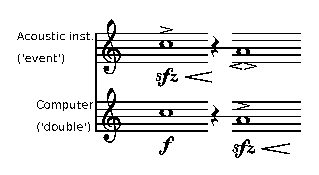
\includegraphics[width=.75\linewidth]{img/lily-interaction}
  \caption[Simplified example of real-time pitch and onset interaction.]{Simple example showing immediate real-time pitch and onset interaction with a second layer of deferred musical dynamic interaction.}
\label{fig:interactive-1A}
\end{wrapfigure}
In the (trivial) example in \hyperref[fig:interactive-1A]{Figure \ref*{fig:interactive-1A}}---a transcription of a fictitious instrument-computer improvisation---the computer `double' follows the pitch and the on/offset times of the `event' in one-to-one mapping. In this regard the response from the computer system corresponds to an immediate and unaltered mirror image. In a second interactive layer, however, the `double' appears to be using dynamic information, i.e. the amplitude envelope, of the note event prior to the current. On the second note in time the `double' mimics the \emph{\textbf{sforzando}}--\emph{\textbf{crescendo}} amplitude curve of the first note of the `event' voice. One may imagine more subtle effects such as introducing temporal tension between the two notes in the domain of timbre; micro-variations in tone colour whose greater shape is asymmetrical, that is unrelated, but whose coming into existence is interactive but deferred in time, etc. The point here is not \emph{what} is done but to show that different compositional strategies\footnote{Working out \emph{what} and \emph{how} in an interactive system in music is tantamount to traditional composition.} may be employed and that interaction may take place on multiple co-existing temporal levels, exploiting different levels of contraction. If, however, the one-to-one mapping of pitch and duration is blurred, if it is not absolutely clear that the `double' is following the `event', that distortion is likely also negatively to influence the deferred time interaction.\label{par:label:human-comp-inter:9} \hypertarget{par:human-comp-inter:9}{If the purpose} in this example (for the moment disregarding the amplitude envelope delay) is defined as \emph{the wish to extend electronically the sound of the acoustic instrument by means of superimposing an electronically generated timbre upon it}, proximity in time is of the essence. A lag or delay in the electronic voice in relation to the acoustic---a delay between `event' and `double'---will create a positively \emph{different} musical gesture compared with the intended effect. If the discrepancy between attack times is sufficiently large, the desired effect of extension of the acoustic sound will fail and the two sounds will instead be perceived as separate musical events. An inconsistent rhythmic displacement may create an interesting gesture but the result is still different from the intention to a considerable degree. The difference between the `double' in \index{real-time}\index{time!real-time}real-time and the `double' in independent time, however, does not merely make up two different tokens of the same type: they constitute two different types of paradigms, two different classes of systems. In essence it is the difference between the extension of an instrument and the extension of a \useGlosentry{glos:musician}{musician}.

%Hence,  Which is not to say that a delay between event and double, between stimulus and response, is not a time for interaction, exchange and negotation. (A time allowing for a different role of the listener?) 

% ``Everything is in motion, eveyrything is changing, everything is % being transformed and yet nothing changes. Such a society, thrown into % technological progress, accomplishes all possible revolutions but % these are revolutions upon itself.''(Baudrillard cited in plant, p. % 35)

\section{Interactive paradigms---\emph{interaction-as-difference}}
\label{sec:inter-parad}
%Context is paramount to the discussion of the significance of rhythmic synchronization. 

As I have attempted to show, \citeauthor{baudrillard02}'s statement that the more perfectly synchronised the `event' and the `double', the lesser the value of the exchange is contestable. Not because it is wrong (I believe it is right), but because, as so often happens, in practice theories rarely play out so symmetrically and because of the particularities of music and time. The importance of \emph{imprecision} \hyperlink{par:human-comp-inter:8-1}{has been discussed} but the aspect of precision may be, depending on the view, equally important. In essence it is a question of context and intention because rhythmic simultaneity and precision may be absolutely critical for some music and equally devastating for others. To explore these issues in the context of interactive computer music, let us consider the important aspect of the purpose as defined in the earlier example in Figure \ref{fig:interactive-1A}: \emph{to extend the sound of the acoustic instrument by superimposing an electronically generated timbre upon it}. This is the intention against which the result is to be measured. It is a simple case of an instrument-computer performance, with a hypothetical, overly simplified, instruction algorithm along the lines of:
%
\begin{equation}\label{eq:1}
  \emph{whatever pitch `heard' $\Rightarrow$ play the same}
\hypertarget{eq:human-comp-inter:1}{}
   \end{equation}
%
Now this could well be a postcard piece by James Tenney\footcites(The \citetitle{tenney04} is a series of eleven short and minimally stated compositions, ``scorecards'' printed on postcards, composed by \citeauthor{tenney04} in the early 1970s.)(){tenney04}[see~also][]{risset87} or an instruction for an improvisation. It is a compositional statement, albeit an open one, but when the rule of synchronicity is introduced as a factor there occurs a major change as far as the freedom and openness is concerned:
%
\begin{equation}\label{eq:2}
\emph{if played note occurs later than original $\Rightarrow$ error}
\hypertarget{eq:human-comp-inter:2}{}
\end{equation}
%
This may also be a viable function to attempt solving the result of which may well be interesting from a musical as well as a technological point of view. Together the two lines form a compositional statement that to a considerable degree limits the independence of the agent to whom these instructions are given. To define restrictions such as these, though it is a perfectly normal musical behaviour, is to issue a control agency. In the Western music tradition where concepts such as \emph{\index{Werktreue}Werktreue}\footcites(The German word \emph{\index{Werktreue}Werktreue} means `to be faithful to the original'. It is commonly used in discussions concerning musical interpretation and musical \index{ontology}ontology.)()[See][3]{benson03}[See also][]{goehr96} have played an important role, the idea that one \useGlosentry{glos:musician}{musician}---usually the composer or the conductor---controls or limits the freedom of another is perfectly normal, in particular from the perspective of those who exercise the `control'.\footnote{Similarly to how the aspect of real-time communication discussed by \citeauthor{baudrillard02}, although despised by him, is intended, desired and profited from by the control agency that governs it.} Furthermore, restricting and reducing the number of choices possible in a given context may promote rather than limit creativity.\footcite[See][chap. 4]{evens05} Regardless of these aspects, however, by adding time to the algorithm---though it is not time \emph{per se} but the values assigned to time in this example---the mode of interactivity is approaching the \hyperlink{sec:inter-defin:par4}{previously discussed} \index{interaction!as control}\index{interaction-as-control}interaction-as-control.

To  complicate this perhaps trivial example, the \emph{role} of the musical `double' in an \index{interaction!interactive music system}interactive music system such as the one described here should be considered. Where does its centre position lie on the `instrument'---`player' continuum?\footcite[For a description of the classification system from which this terminology is borrowed see \autoref{sec:music-pract-inter}. See also][]{rowe01} 
%Section
That is, to what extent is the `double' also able to contribute actively to the music as opposed to merely following instructions? By no means is this a simple distinction to make, nor are `player' and `instrument' separate and irreconcilable categories. Any instrument, \index{digital}digital or analogue, electronic or acoustic, will contribute to the music through its history, its physicality and its limitations as well as through many other parameters. The seemingly opposing paradigms of `player' and `instrument' are perhaps best described as related classes with many common members where the `player' class \emph{extends} the functionality of its parent `instrument' class (a `player' will need some kind of an `instrument' on which it  `plays'). Perhaps the process of categorising a system within these classes will have to be done pragmatically, not based on the properties of the computer and its \index{software}software, but rather on the \emph{usage} and \emph{purpose} of (using) it. If I have a distinct intention about \emph{when}, with \emph{what}, and \emph{how} I want my computer to respond (musically), then I am essentially designing an `instrument'. If, on the other hand, I am primarily interested in engaging in a mutual exchange with the computer, then I am essentially implementing a `player'. In this context the consequential difference between the two methods is that the latter has only a vaguely formulated, system-specific, rationale against which the output may be evaluated,\footnote{If the played note by a given `player', that implements the rule in \hyperlink{eq:human-comp-inter:1}{a quasi algorithm \eqref{eq:1}}, is not equal to the most recent note analysed, it only means the current played note is not the most \emph{recent} note analysed, which is not an error according to the rule. The most recent note analysed may appear at some later point in time.} one where there is room for interpretation and difference. The former, on the other hand, includes preconditions that make possible an unambiguous evaluation of the output in relation to the input (such as the \hyperlink{eq:human-comp-inter:2}{second rule above}).

The `instrument' paradigm, in the sense that it takes input from a source from which it generates an output based on a logical rule set, is a type of communication system. Information is sent from \useGlosentry{glos:musician}{musician} (sender) to `instrument' (receiver), and the sender expects to be in control of the system, i.e. expects that messages transmitted are received with a minimum of noise and that the system is able to decode the message correctly. In this description is also an expectation that the code does not change over time, a potential for developing a fluency on the instrument. \emph{\index{interaction!as control}\index{interaction-as-control}Interaction-as-control}. Within the `player' paradigm the streams of communication are not unidirectional. The code of the communication may in part be negotiated in the course of action. The value and meaning of noise are different. A `player' system approaches a circular cause-and-effect system, a container for feedback, a \index{cybernetics}cybernetic system. If what comes out of it is not satisfactory according to some standard---a standard imposed and set in runtime rather than, as is the case with an `instrument', pre-runtime---it is up to either part to alter its behaviour and attempt to create the desired change to approximate the criterion, to initiate a big enough difference to modify the balance and cause a system change. \emph{\index{interaction!as difference}\index{interaction-as-difference}Interaction-as-difference}. Despite the reductive way the two paradigms `instrument' and `player' were portrayed by the simplistic rules in the \hyperref[sec:inter-parad]{examples above}, I believe they bear evidence of the different kinds of interaction they encourage. It is equally true, and important to remember, however, that the same system may in fact display different characteristics depending on the posture of those who engage interactively with it. This is not the sole property of electro-acoustic instruments, but just as true for any musical instrument.

%Though it is possible here, as well as in the former system, to measure the information content in the communication, without the formal, predetermined rules, without the code, the simple logic (if $x$, then $y$)former system \emph{may} be used here but the data validation process is considerably more complex. 

%These systems are still abstract models. The point here is not to discuss the possible implementation, though it should be mentioned that the `player' system, fully expanded would constitute a very complex system. As models they portray differences where the most conspicuous is that status of noise and error. In the first noise should be avoided and errors are identifiable. In the second noise is par of the message and errors are generally indeterminable.

%The consequences of the latter is also that I must accept `faulty' or unexpected output from the computer, and `errors' or noise in my `signal' should preferably not cause a system havoc. 

In the discussion above I have attempted to reveal the compound nature of the matter of interaction and time. Within it are concealed issues relating to causality, embodiment, expression, social exchange, the Other, and many, many more. The question I have tried to address here is how and if the \index{real-time}\index{time!real-time}real-time interaction of communication is related to the \index{real-time}\index{time!real-time}real-time of \index{interaction!musical}musical interaction and an unwrapping of some of the different kinds of time at play. As was mentioned towards the end \hyperlink{par:human-comp-inter:10}{of Section \ref*{sec:time-interaction}}, \citeauthor{baudrillard96}'s point is that what he calls symbolic exchange, essentially \index{interaction!social}social interaction, depends on time; it feeds on the suspense that is the result of the delay between cause and effect, whereas the \index{real-time}\index{time!real-time}real-time of the \index{virtual}Virtual is the effectual abolition of both time and distance. For the moment disregarding the fact that a different analysis of communication and time in the sphere of the \index{virtual}Virtual is possible,\footcite[E.g.][chap. 11]{levy97} it is obvious that the relation between time and meaning is of a different kind when the realm of musical performance is entered. The thought that expression and `meaning' would increase with \emph{\useGlosentry{glos:latency}{latency}} in a musical instrument is preposterous. (It would make the church organ the most expressive instrument and something like the violin the least expressive.) Further, the time and rhythm of \index{interaction!social}social interaction are even more pertinent and present in music and I have argued that, even if the interaction (in music) is limited to a simple trigger-response metaphor of communication, time is still at play, by the very nature of music. For a traditional musical instrument the interaction between it and the musician is governed by the \index{real-time}\index{time!real-time}real-time information (feed-back) but \emph{also} by the musician's embodied knowledge about playing that particular instrument design, and by the intellectual memories of playing and learning how to play (and a myriad of other memories). Therefore, even if it seems like the playing is taking place in \index{real-time}\index{time!real-time}real-time, many other kinds of time and interactions are taking place on lower levels. Some of this knowledge is more or less consciously encoded into memory and some of it is entirely beyond control and influence.
%, such as deterioration of the instrument, physical proerties of the room we are in, psychological changes, etc.


%In practical terms: I don't have to re-learn how to play the saxophone when I pick up a new instrument, one I have never played before, because the interactive knowledge is not tied to the specific object but to the general concept of the instrument.



%The perhaps most pressing question is what the relation is between human-computer interaction outside of the field of musical practice and musican-computer interaction inside that field. 

\section{Multiplicities of musical interaction }
\label{sec:mult-music-inter}


\hypertarget{sec:human-comp-inter:par8}{The development} that led to the \index{real-time}\index{time!real-time}real-time responsive computers discussed \hyperref[sec:interaction-time]{above} unquestionably gave birth to the possibility of a different mode of interaction, and the distinction between the prior, non-real-time interaction and the current \index{real-time}\index{time!real-time}real-time is relatively obvious. Reading \citeauthor{baudrillard96}'s \citetitle{baudrillard96:writing}, however, one may get the impression that \index{real-time}\index{time!real-time}`real-time' is a unanimous and clear-cut category of interaction. Between \index{real-time}\index{time!real-time}real-time and detained time, between high-definition and low-definition time, however, exist many layers of interactions that operate on different timescales, particularly in music. Ingrid \citeauthor{monson96}'s book \citetitle{monson96} takes this multi-layered nature of \index{interaction!musical}musical interaction (of jazz and improvised music) as its starting-point: ``Stressed here are the reciprocal and multi-layered relationships among sound, social settings, and cultural politics that affect the meaning of jazz improvisation in twentieth-century American cultural life''.\footcite[2]{monson96} Sounds do not interact in a void but depend on and become influenced by social and culturo-political interactions. She also makes use of the linguistic model of \index{interactional texts}\index{Monson, Ingrid!interactional texts}\index{interaction!interactional texts}`interactional texts', briefly 
\hyperlink{sec:inter-defin:monson}{discussed above}, which allows us to identify the multiplicity and simultaneity of musical communication, as many of these `texts' may operate concurrently. \citeauthor{monson96} writes that ``the intersection of all of these roles [\ldots] contributes to the way in which interactionally produced musical texts develop'' and that ``these interactionally produced events structure both musical and social space''.\footcite[189-90]{monson96} \citeauthor{monson96} assembles different modes of interactivity and shows that these are all part of, and present in, the musical performance. The minute adjustments made within the jazz rhythm section to accommodate the groove may at the same time seem enigmatically indulgent\footcite[For a study on the rhythmic variation present in jazz, see][]{friberg02} and incredibly sensitive to variation. On one level, the interaction within the rhythm section certainly takes place in very high definition and it must be said to conform with what \citeauthor{baudrillard02} calls the inexpiable `live' time. Along with this \index{real-time}\index{time!real-time}real-time interaction, however, are many other levels of interdependent interactions such as those formed by interpersonal relations, as mentioned by \citeauthor{monson96}. These manoeuvre in a different time but may well influence, and depend on, the lower level \index{real-time}\index{time!real-time}real-time interactions.

Is this not true also for \index{interaction!human-computer}\index{HCI}human-computer interaction? That the social and political interactions that relate to the different aspects of technology inform not only the technology itself but also how one interacts with it? Or is the nature of the `virtual', digitally encoded as it currently is, so radically different from the social dimension---the `world' as \citeauthor{baudrillard02} would refer to it---that, in the encounter, any formerly constructed interactive texts are inescapably eradicated and all that remains is the  \index{real-time}\index{time!real-time}real-time \index{virtual}virtual representation? The deceptive distinction between \index{real-time}\index{time!real-time}real-time and non-\index{real-time}\index{time!real-time}real-time mentioned above is mirrored in an equally deceptive distinction between real and \index{virtual}virtual. Now this is irrefutably one of \citeauthor{baudrillard02}'s main points,\footnote{Hyperreality is the process of making the representation of the world more real than the real world, hence making it difficult to distinguish the real from the virtual.} but for him, although one may be mistaken for the other, the real and the \index{virtual}virtual are mutually exclusive: ``for it is the particularity of the \index{virtual}virtual that it puts an end not just to reality, but to the imagining of the real, the political and the social; not just to the reality of time, but to the imagining of the past and the future''.\footcite[107]{baudrillard02} As the extension of \index{hyperreality}hyperreality the \index{virtual}virtual scrambles and destabilises truth and the real. Eventually the \index{virtual}virtual claims the real, for there ``is no room for both the world and its double''.\footcite[34]{baudrillard96} As was mentioned earlier in relation to the Situationist's notion of the \index{Spectacle, Society of the}\index{Debord, Guy!Spectacle}Spectacle, \citeauthor{baudrillard96} states that there is no escape from the \index{virtual}virtual because it keeps no trace of the real, of the earlier world. This, he says, makes it a hypothesis with much more far-reaching consequences than \citeauthor{heidegger93}'s notion of \emph{\index{Heidegger, Martin!enframing}enframing} because, just as there is a possibility for reversal in Debord's description of the \index{Spectacle, Society of the}\index{Debord, Guy!Spectacle}Spectacle, \index{Heidegger, Martin!enframing}enframing is both ``\emph{danger} in the highest sense''\footcite[333]{heidegger93} and holds within it the potential for ``the rising of the saving power''.\footcite[338]{heidegger93}

\section{Interaction and the Digital}
\label{sec:interaction-digital}


\hypertarget{interaction-digital}{The cross-disciplinary scholar Aden \citeauthor{evens05}}, in a chapter of his book \citetitle{evens05} entitled ``The  Question Concerning the Digital'', approaches \citeauthor{heidegger93}'s ponderings on technology, but, as can be told from the title, centres on the \emph{digital} as a defining property of modern technology, as its uniting power. Because the \index{digital}digital is the code which allows for the representation to be infinitely reproduced, because it introduces order, consistency and generality into the world, \citeauthor{evens05} identifies the \index{digital}digital as a result of the technology's \index{Heidegger, Martin!enframing}enframing\footnote{The German word used by \citeauthor{heidegger93} is \emph{Gestell}, which is commonly translated as \emph{enframing}. Aden Evens, however, suggests the English translation should be \emph{set upon}, which is what he uses consistently. \cite[See][182n2]{evens05}. In the translation of \citetitle{heidegger93} that I am using, however, a distinction is made between \emph{setting upon} and \emph{enframing}.} of nature. Truly, the binary system is an excellent example of generality, the ultimate abstract code which chops up nature in infinitesimal slices (frames?), each of which is further sliced up and every `bit' is assigned a zero or a one. The represented object is not just reproducible, it is comparable (a binary distinction for each bit) and communicable (a stream of numbers is easy to transmit). It is \index{digital}digital. \citeauthor{evens05} distinguishes the \index{digital}digital as ``purely formal'' and as such it ``grasps only form and so falls ever short of actuality''.\footcite[66]{evens05}  As was \hyperlink{sec:human-comp-inter:par5}{mentioned earlier}, according to \citeauthor{baudrillard02} the commodity has gone through a process of complete and total abstraction, an annihilation of meaning, whereafter it signifies only itself. \citeauthor{evens05} makes the connection\footnote{Aden \citeauthor{evens05} refers to \citeauthor{baudrillard02}'s \index{digital}digital interpretation of the Twin Towers in New York City.} and points to the singular nature of the \index{digital}digital and its inability ever to point beyond the plane of the \index{digital}digital: ``It represents but does not present''.\footcite[76]{evens05} In his text the \index{digital}digital is given a thorough and very readable investigation, expanding the concept well beyond a mere binary system of digits. \citeauthor{baudrillard96}'s \index{virtual}virtual/real dichotomy, mirrored in \citeauthor{evens05}'s \index{digital}digital/actual, is because of the multiple perspectives provided by \citeauthor{evens05} (represent/present, general/singular) considerably blurred. But the more important distinction here is that, whereas \citeauthor{baudrillard96} finds the \index{virtual}virtual transformation immutable, although \citeauthor{evens05} identifies serious limitations of the \index{virtual}`virtual' (limitations he traces back to the formality of the \index{digital}digital), he also sees the possibility for it to transcend its own medium and become a dynamic and ``organic aggregate''.\footcite[78]{evens05} When \citeauthor{baudrillard02} sees the `sampling' of our world as irrevocable and a sign of the complete failure of Heidegger's quest to hold the dangers of technology before our eyes, \citeauthor{evens05} traces Heidegger's notion of the \emph{saving power} of technology to the \emph{interface} between \index{digital}digital and actual. Further obscuring the \index{digital}digital/actual boundary, \citeauthor{evens05} states that: ``the digital is not on its own, as it engages constantly with the human world of actuality''. It engages with the world, through humans, mediated by the interface between the \index{digital}digital and the actual. Perhaps one could say that in this process, the \index{digital}digital representation of the world is `de-framed'. \citeauthor{evens05} argues that ``whatever vitality, whatever creativity inheres in digital technologies, [\ldots] will be found in [the] interstitial zone''; the fuzzy boundary of the \index{digital}digital.\footcite[79]{evens05}

\label{sec:interaction-digital-1}
The interface, as discussed \hyperref[sec:human-comp-inter]{above}, allows access to technology and the activities involved constitute the human-technology interaction. According to \citeauthor{evens05} the space between the \index{digital}digital and the actual, the ``ambiguous space of transformation'',\footcite[80]{evens05} is a space occupied by the interface, or by the technologies that make up the interface (the mouse, the keyboard, the icons on the screen, etc.). So the (\index{digital}digital) content is challenged by the user through the interface. But where do the data end and the interface begin? (The conflation between text and link in hypertext is an example of the difficulty in delimiting data from interface: the text is both content \emph{and} interface.) And by what standard is the (\index{digital}digital) computer interface \emph{less} \index{digital}digital than the data it makes available? If it too is purely \index{digital}digital, in what way does it open a channel to the data that makes it more accessible to the sphere of the actual, more alive? \citeauthor{evens05} maintains that, because the interface mediates between the user and the computer, it is by definition a hybrid of both \index{digital}digital and actual, but the hybrid is accomplished, not by making the (already \index{digital}digital) interface more actual, but by the user submitting to the formal reduction of the \index{digital}digital.\footcite[80]{evens05} In order to move across the actual/\index{digital}digital boundary one has to succumb to the \index{digital}digital and herein lies the danger, the threat, of the \index{digital}digital: ``by requiring each user to conform to its standards, it imposes a uniform experience that not only reduces the world to a pure formality but offers to each of us the same formalities, the same possibilities, the same pseudo-creativity''.\footcite[81]{evens05} This twofold nature of the \index{digital}digital as both potential and threat is a reflection of \citeauthor{heidegger93}'s ruminations on the \emph{dangers} and the \emph{saving powers} of technology. By reference to German poet Friedrich H\"{o}lderlin, \citeauthor{heidegger93} claims that the two aspects are never mutually exclusive but always potentially co-existent.\footcite[The lines by H\"{o}lderlin are: ``But where danger is, grows / The saving power also''. Quoted in][333]{heidegger93}

\label{sec:interaction-digital-2}
Therefore, the interface allows for interaction, and following \citeauthor{evens05}, it binds together the user and the computer; a glue without which the \index{digital}digital would remain inaccessible. Metaphorically speaking, the interface \emph{creates} interaction. This model gives the impression that the user \emph{is} the actual and the computer \emph{is} the \index{digital}digital and that these two agents are utterly incompatible unless one approaches the other. Because the \index{digital}digital is static and unchangeable, trapped in its own formality, of the two only the user, i.e. the human, is capable of altering him/herself to approach the \index{digital}digital through the interface. As a consequence, has the user ceased to be \emph{only} actual? \hyperlink{sec:inter-defin:par4}{Going back} to the concept of \index{interaction!as control}\index{interaction-as-control}interaction-as-control, common to much of \index{interaction!human-computer}\index{HCI}human-computer interaction, given the \index{digital}digital/actual dichotomy so thoroughly explored by \citeauthor{evens05}, in order for the user to exercise control over the computer s/he has to become the computer to a certain extent, give something up, give in to gain. (To gain, because, after all, something is returned or computers would not sustain such interest.) This duality is identified by McLuhan when he states that ``any technology is an extension or self-amputation or our physical bodies'',\footcite[49]{mcluhan01} paraphrased and extended by \citeauthor{baudrillard02} to the somewhat more radical and acrimonious ``[technology is the] expulsion of man''.\footcite[35]{baudrillard96} Is the reconfiguration demanded by the user, as the prerequisite for \index{interaction!human-computer}\index{HCI}human-computer interaction, a staging of this extension/amputation/expulsion? Is the giving up of a part of our selves in order to embrace technology\footcite[McLuhan writes that to ``behold, use or perceive any extension of ourselves in technological form is necessarily to embrace it''.][49]{mcluhan01} really specific to interaction with technology? Is the request of the \index{digital}digital that we give in, just a little bit, to its mode of operation not a natural component of any kind of interaction? I \emph{approach} the other in the interactive invite by `reconfiguring' my senses to her, albeit slightly, give up a part of my \index{Self}self and, in the process, I also extend myself.

\label{sec:interaction-digital-3}
Towards the end of ``The Question Concerning the Digital'' the very interesting idea of ``a dialectic of interface and data [that] also implicates the user''\footcite[80]{evens05} is introduced. As the interface is refined, argues \citeauthor{evens05}, the \index{digital}digital data are forced to reorganise and the users, for their part, keep pressure on the interface and the \index{digital}digital, which, in this operation, is pushed to become more than it is,  challenged, and ``the pipe that passes from the \index{digital}digital to the actual bursts its seams to carry the \index{digital}digital beyond itself''.\footcite[81]{evens05} These thoughts open up an alternative, less machine-centric view on how to think about and attempt to understand technology/virtual/\index{digital}digital. I argue that in the dialectic of interface, data and user the interaction is the central aspect. The interaction \emph{creates} the interface. A `good' interface is one that allows itself to be created.\footnote{The most obvious and tangible example within the realm of computer music is the \index{Pure Data (PD)}\index{Puckette, Miller}Pure Data (PD) by Miller Puckette. Its interface is recreated for every instance, every project, every interaction, every iteration. \cites[See][]{puckette96}[and][]{puckette07}.} In this model the user does not constitute the actual, s/he is primarily \emph{part of} it and similarly the computer is primarily \emph{part of} the \index{digital}digital. Actual and \index{digital}Digital are two types, two classes that can have any number of members and whose structure is somewhat amorphous. The more the agents of different classes interact with each other, the more the two classes overlap and the more they inherit properties from each other and the larger, less rigid and more fluent becomes the interface: the union between the two classes. The more `information' one class has about the other, the more likely is the interactive field to grow. The more rivalry there is the more likely it is to vanish. Knowledge about the Other is the key to avoiding fear and conflict.

\label{sec:interaction-digital-4}
In this section the Real/\index{virtual}Virtual opposition favoured by \citeauthor{baudrillard02} has been compared with Aden Evens's Actual/\index{digital}Digital distinction, a dichotomy that consists of categories that may be slightly misleading and not as clear cut as they appear. The \index{digital}Digital is used by Evens in an attempt to avoid the technology and instead focus on the structure of technology. This is comparable to how Heidegger points to the \emph{essence} of technology rather than technology itself which, in both cases, allows for philosophical rather than a technical discussion. The `Actual' as category is the negation of the \index{digital}`Digital' and silently points to Heidegger's `truth' or `nature'. But is the \index{digital}digital encoding a property of technology only? What is a fired neuron in the brain if not a binary transition? In a discussion on cybernetics Gregory Bateson writes that ``in the vast majority of instances, the neuron either fires or does not fire'' and he goes on to explain how ``it is possible to make systems out of \index{digital}digital neurons that will have the \emph{appearance} of being analogic systems''.\footcite[103]{Bateson} In other words, according to \citeauthor{Bateson}, the human brain has certain low-level qualities that may be seen to lean towards the \index{digital}digital. Similarly, through the use of artificial neural networks, it is possible to simulate an analogue system by \index{digital}digital means. This affinity between categories makes it possible to look at \index{interaction!human-computer}\index{HCI}human-computer interaction in a way less focused on opposition and resistance and more on exchange. Described as classes, the \index{digital}digital and the actual can reciprocally exchange properties or modes, without losing their mutual identity. Furthermore, instances of these classes---the agents of the interaction---construct the interface through which data may pass and in these inter-agent transactions the participants have to acknowledge each other.

%Although the `Real' must be understood in relation to a philsophical context as `truth' or `nature' and thereby outside the scope of this discussion, the `Virtual' as a place where technology interaction takes place is problematic. In what constist the difference between a dream and 

\section{Interaction and symbiosis: Cybernetics}
\label{sec:interaction-symbiosis}

%The important aspect of time and interaction, also discussed \hyperref[sec:interaction-time]{in section \ref*{sec:interaction-time}} is 

%Apart from the discussion on \ref{sec:inter-defin:par4}musical interaction and the briefly mentioned debate on intelligent agents

Before the \index{digital}digital revolution, and some twenty years before the \index{PC}\index{Personal Computer}PC, Joseph Licklider---whose significant work was briefly mentioned \hyperref[sec:human-comp-inter]{above}---imagined the future of \index{interaction!human-computer}\index{HCI}human-computer interaction and computation as one devoid of ``inflexible dependence on predetermined programs'' where computers and humans would develop a symbiotic relation. In \citeauthor{licklider60}'s vision the computer usage paradigm would shift from the user supplying the computer with a pre-formulated problem to one in which the user and the computer ``cooperate in making decisions and controlling complex situations''.\footcite{licklider60} Although \citeauthor{heidegger93}, \citeauthor{baudrillard02} and \citeauthor{evens05} have focused on the problems of the dissimilarities and incompatibilities between technology and its users they have all to various degrees considered the dangers and the subsequent destructive aspects of technology and pondered on ways in which it may be altered, to become more human, \citeauthor{licklider60}, while identifying the same dissimilarities, saw great potential in them. To \citeauthor{licklider60}, the human-computer incongeniality was a possibility rather than an obstacle, a possibility for computers to complement humans in difficult and perhaps mundane tasks. His categorization of the two parts of a human-computer system is a rough summary of the challenges involved in human \index{interaction!computer}computer interaction:

\begin{squote}
As has been said in various ways, men are noisy, narrow-band   devices, but their nervous systems have very many parallel and   simultaneously active channels. Relative to men, computing machines   are very fast and very accurate, but they are constrained to perform   only one or a few elementary operations at a time. Men are flexible,   capable of ``programming themselves contingently'' on the basis of   newly received information. Computing machines are single-minded,   constrained by their ``pre-programming''. Men naturally speak   redundant languages organised around unitary objects and coherent   actions and employing 20 to 60 elementary symbols. Computers   ``naturally'' speak non-redundant languages, usually with only two   elementary symbols and no inherent appreciation either of unitary   objects or of coherent actions.

To be rigorously correct, those characterizations would have to   include many qualifiers. Nevertheless, the picture of dissimilarity   (and therefore potential supplementation) that they present is   essentially valid. Computing machines can do readily, well, and   rapidly many things that are difficult or impossible for man, and   men can do readily and well, though not rapidly, many things that   are difficult or impossible for computers. That suggests that a   symbiotic cooperation, if successful in integrating the positive   characteristics of men and computers, would be of great value. The   differences in speed and in language, of course, pose difficulties   that must be overcome.\footcite[Section 3.1]{licklider60}
\end{squote}

The language problem---which in this context is an issue of information encoding and hence related to the \hyperlink{interaction-digital}{discussion of the \index{digital}digital}---cannot be said to have been overcome. Computers still do not generally ``speak'' redundant languages and even if higher-level computer languages have been developed, these are far from spoken inter-human communication. Further, if the computer according to \citeauthor{licklider60} was too fast in 1960 (for the purpose of symbiosis), considering that the input devices are roughly the same whereas the computer speed capacity according to Moore's law has doubled 32 times since then,\footnote{Gordon Moore predicted in 1965 that the number of transistors on a computer chip, and hence the processing power, would double every 18 months ($1960\Rightarrow2008=48$ years, $\frac{48\times12}{18}=32$). To be fair, Moore's law was not formulated until 1965 and in reality it seems as if the doubling has actually happened on average every 20 to 24 months. All the same, computers have grown much faster and the means for interaction has not changed in any radical way.} speed according to the same standard must still be an issue. Despite these issues concerning speed and language, however, are we not already living the \index{symbiosis, man-computer}man-computer symbiosis predicted by \citeauthor{licklider60}?

On the one hand it is fair to say that we are. We are living interdependently and in close union with computers in what could be called a symbiotic relationship. (After all is not the greatest fear, the most commonly explored horror of science fiction, that one day computers may not need us?) To deal with the speed issue, \citeauthor{licklider60} envisioned resource distribution by means of time-sharing that implemented `thinking centres', the equivalent of ``present-day libraries'', where one machine can serve multiple users (in essence a client/server protocol). With striking accuracy he draws the outlines of that which is to become the Internet: ``The picture readily enlarges itself into a network of such centers, connected to one another by wide-band communication lines and to individual users by leased-wire services''.\footcite[Section 5.1]{licklider60} The Internet as a thinking centre in a symbiotic relation with humans. In a search of the Internet not only answers are produced; just as many new problems are formulated. Though in reality it is arguable whether the Internet and the typical use of the Internet would qualify as one part in a symbiotic relation, the Internet in the sense of information collection was one of the aspects \citeauthor{licklider60} envisioned as part of \index{symbiosis, man-computer}man-computer symbiosis.

On the other hand, judging from Steve Dietz's paper \citetitle{dietz02}, in which the first dream is \citeauthor{licklider60}'s dream of \index{symbiosis, man-computer}man-computer symbiosis, we are still far from that vision. As one of the curators\footnote{Another curator was Electronic Music Foundation founder and president Joel Chadabe.} for the \emph{2003 New York Digital Salon}\footcite{digitalsalon03} \citeauthor{dietz02} examines ten dreams of technology that are not yet `true' or `real' (outside the realm of art, one may add), but which all have a future, ``even if we do not yet know what it is and despite the certainty with which it is predicted''.\footcite{dietz02} \hypertarget{sec:target:interaction-symbiosis}{Though many artists} have dreamed the dream of symbiosis, the artwork \citeauthor{dietz02} associates with man-machine symbiosis is David \citeauthor{rokeby91}'s installation \citetitle{rokeby91}. As an interactive installation\footcite[For an introduction and description of the work, see][]{rokeby91} it engages with the visitor in a sophisticated feedback process. The visitor places objects, toys and household objects that the computer `sees', analyses and assign names to. Over time it builds relations between the objects and, through the use of speech synthesis, it starts building phrases out of its repository of the object/name couples that it reads back to the visitors.

In \citetitle{rokeby91}, the visitor and the computer interact through (are mediated by?) the objects and through the voice of the speech synthesis engine. By placing objects in the computer's line of sight the visitor teaches it something about the world and through the computer's accumulated knowledge, the visitor is told something about the world from a slightly skewed perspective. As regards the topic of interaction, though there are many interesting aspects of \citetitle{rokeby91} that intersect with the discussions in the current text, the \hyperref[sec:interaction-time]{question of time} (see also the discussion relating to \hyperlink{sec:human-comp-inter:7}{\index{real-time}\index{time!real-time}real-time \index{interaction!musical}musical interaction}) is particularly well illustrated. \citeauthor{baudrillard02}, who obviously felt strongly about this, pointed to the \index{real-time}\index{time!real-time}real-time aspect of the \index{virtual}virtual as inexpiable: ``it is the particularity of the \index{virtual}virtual that it puts an end not [\ldots] just to reality of time, but to the imagining of the past and the future''.\footcite[107]{baudrillard02} It is the immediate return, the expeditious reply, that kills the past and the future and turns everything into a singular moment. Whether one agrees with \citeauthor{baudrillard02} or not, the concept of \index{real-time}\index{time!real-time}real-time must be expanded beyond its use in \index{interaction!human-computer}\index{HCI}human-computer interaction because, as was seen towards the \hyperlink{par:human-comp-inter:8}{end of Section \ref*{sec:time-interaction}}, \index{real-time}\index{time!real-time}real-time interaction, the instantaneous proximity of events, has crucial significance in \index{interaction!musical}musical interaction. Within the realm of computers there are several different types of \index{real-time}\index{time!real-time}real-time; there is the \index{real-time}\index{time!real-time}real-time interaction as well as the related but yet different aspect of \index{real-time}\index{time!real-time}real-time computation. \index{real-time}\index{time!real-time}Real-time interaction depends on \index{real-time}\index{time!real-time}real-time computation but the latter does not necessarily have to implement the former. 

As a system, \citetitle{rokeby91} relies on a number of different interactive modes of which \index{real-time}\index{time!real-time}real-time computation is one of the important ones. Without it, the project would not have been possible: The computer would not have been able to process the images from the camera (constituting its `line of sight'), nor would it have been able to `read' the texts back to the visitors. Yet the communication between the visitor and the \index{virtual}virtual world of the installation does not take place in the kind of one-dimensional click-and-response \index{real-time}\index{time!real-time}real-time that \citeauthor{baudrillard02} objects to. Rather, because of the way the \index{software}software accumulates `knowledge' about objects displayed to it over time, the communication is based on present \emph{and} past experiences, not just the current. Therefor, the interaction only becomes meaningful if both parties accept that they engage in the exchange coming from different backgrounds and that mutual respect for this past is shown. \hyperlink{sec:inter-defin:par4}{\index{interaction!as control}\index{interaction-as-control}Interaction-as-control} is not possible, not meaningful, because the main interactive mode is based on exchange, feedback and reciprocity on a number of simultaneous layers of time. As \citeauthor{dietz02} writes: ``The symbiotic feedback loop infers that over the course of more than a decade, the computer `learns' more and more about the world, and its oblique, almost Delphic utterances of our mundane combinations of boot and rubber-duck-and-ball objects also causes us to perceive the world differently''.\footcite{dietz02}

\citetitle{rokeby91} and the idea of man-machine symbiosis are in essence \index{cybernetics}cybernetic ideas. As a discipline and a meta-theory cybernetics is concerned with (among other things) ``control and communications in the animal and machine'',\footcite[There are many definitions of cybernetics---this one is from Norbert Wiener's \emph{Cybernetics} (1960), as cited in][]{cybernetic08} by themselves and together. \citeauthor{licklider60} defined one of the main aims of \index{symbiosis, man-computer}man-computer symbiosis as the wish to go from systems that solved pre-formulated problems to systems that, in a symbiotic relation with a user, would (also) act by themselves and contribute to the formulation of the problem.\footcite{licklider60} If we define these as belonging to two categories of systems (non-symbiotic and symbiotic), one of the differences between them may be described in terms of energy. The non-symbiotic system accepts input given to it and responds according to some (pre-defined) logic. It is a causal system in which the energy is provided by the user. The user energises the system by posing the question, much like when a billiard ball strikes another and the motion energy is transferred from the former to the latter.\footcite[405]{bateson72:cyber} In the symbiotic system, on the other hand, ``the energy of the response is usually provided by the respondent. [\ldots] when a neuron fires another, or an impulse from a microphone activates a circuit, the sequent event has its own energy sources''.\footcite[409]{bateson72:cyber} Gregory \citeauthor{bateson72:steps} distinguishes this last category as a \index{cybernetics}cybernetic system, a communicational system with sequences resembling stimulus-response rather than cause-and-effect.\footcite[409]{bateson72:cyber} Feedback rather than click-and-response. Reciprocity rather than immediate reaction.

Again, it should be pointed out that in practice the difference between these types of systems is far from unequivocal, but, though there is nothing to say that a cause-and-effect system cannot incorporate some idea of time and memory, i.e. the system type itself does not exclude time, a \index{cybernetics}cybernetic system depends on it. Even the simplest \index{cybernetics}cybernetic unit displays ``a sort of determinative \emph{memory}'', because the ``stability of the system (i.e. whether it will act self-correctively or go into runaway) depends upon transformations of difference''.\footcite[317]{bateson72:cyber-self} Every part of the system will respond to changes and bits of information are passed around. Every such bit is ``definable as a difference which makes a difference'' and such differences are successively transformed through the internally interactive system.\footcite[315]{bateson72:cyber-self} In other words, the \index{cybernetics}cybernetic system needs to know, to remember, its state prior to current time and, preferably, have some notion of what the state of the other parts of the system is: it interacts internally with itself and with its environment. According to \citeauthor{bateson72:cyber-self}, these properties are what gives a \index{cybernetics}cybernetic system its holistic and mental features and his conclusion, of great interest from the point of the current project, is summarised in the following statement: ``[I]n no system which shows mental characteristics can any part have unilateral control over the whole. In other words, \emph{the mental characteristics of the system are immanent, not in some part, but in the system as a whole}''.\footcite[p. 316 (Italics by the author.)]{bateson72:cyber-self} Hence, in an interactive system in music that deploys some notion of cybernetics, the computer must not be seen as an isolated `player' but as part of a whole that includes the performer(s) with whom the system is interacting. Furthermore it will not be possible for the performer to gain control over the computer, or the computer over the performer, without the system failing or regressing. \index{interaction!as control}\index{interaction-as-control}Interaction-as-control relinquished in favour of \index{interaction!as difference}\index{interaction-as-difference}interaction-as-difference.

\section{Time and interaction revisited}
\label{sec:time-inter-revis}

\hypertarget{sec:target:time-inter-revis}{That} \citeauthor{baudrillard02}'s critique of \index{real-time}\index{time!real-time}real-time, however easily accepted, is not a property specific to the \index{virtual}Virtual \hyperlink{par:human-comp-inter:10}{has already been argued}, and I believe the brief analysis of \citeauthor{rokeby91}'s installation further corroborates it. More than anything the \index{real-time}\index{time!real-time}real-time of \citeauthor{baudrillard02} is a property and result of a general view of interaction, deflated and overly simplified by the all too common  and absurd notion of consumerism that `one-click-shopping' has given rise to. As a European inheritor of the visions of Joseph \citeauthor{licklider60}, Douglas Engelbart \footnote{D. Engelbart is commonly recognised as the inventor of the computer mouse, hypertext and ARPANET, the precursor of the Internet. Like \citeauthor{licklider60} in the early 1960s he argued for the use of computers to augment the human intellect. \parencites()()[See][viii]{levy97}[See also][]{johnson97}} and Marshall McLuhan,\footcite[See the foreword to][by R. Bononno]{levy97} French sociologist Pierre \citeauthor{levy97} whose visionary ideas on collective interaction were mentioned at \hyperlink{sec:target:inter-defin:par6}{the end of Section \ref*{sec:inter-defin}}, voices related criticism of the ``staccato, accelerated, quasi-punctual temporality of `interactivity'''.\footcite[125]{levy97} His book \citetitle{levy97} is concerned with opportunities and perils in network communities and nomadism made possible by the information highway. He supports the idea of multiple time configurations as well as the necessity of separating \index{real-time}\index{time!real-time}real-time, i.e. the sensation of time that emanates from interacting with \index{real-time}\index{time!real-time}real-time technologies, from the ``time experienced by the imagining community'' which will always overflow the the ``inadequacy of the immediate, of amnesiac channel hopping''.\footcite[125]{levy97} In other words, attempting to separate technology from the expression of technology.

I have now remarked several times on how interaction takes place in a \hyperlink{sec:human-comp-inter:par8}{multi-layered fashion} rather than in a singular type of interactional time, as is exemplified in some cases of \index{interaction!computer}computer interaction as well as \index{interaction!musical}musical interaction, and I have also suggested that the focal point of \citeauthor{baudrillard02}'s critique of the \index{real-time}\index{time!real-time}real-time interaction the \index{virtual}Virtual lies outside of the \index{interaction!human-computer}\index{HCI}human-computer interaction axis---and briefly hinted at \citeauthor{levy97}'s apparent support of this notion---but I return to the subject once again, for I believe it is one of the most important, and one of the most complex, aspects of music, let alone interactive music. Although Pierre \citeauthor{levy97} offers no consolation with regard to an actual, practical solution---I doubt that it is possible to find a solution that has relevance outside the realm of a specific context---he does provide a description of both the vision and the challenges of an understanding of time in a computer-mediated collective community:

\begin{squote}
The inadequacy of the immediate, of amnesiac channel hopping, no longer leads to lengthy sequences of interpretation, the infinite patience of tradition, which encompasses in a single sweep the ages of the living and the dead, and employs the quick currents of the present to erect a wall against time. [\ldots]

The rhythm of the imagining community resembles a very slow dance, a slow-motion choreography, in which gestures are slowly adjusted and respond with infinite precaution, in which the dancers gradually discover the secret \emph{tempi} that will enable them to shift in and out of phase. Each learns from the others how to make their entrance in stately, slow, and complicated synchrony. Time in the intelligent community spreads itself out, blends with itself, and calmly gathers itself together like the constantly renewed outline of the delta of a great river. The imagining collective comes into being so that it may take the time to invent the ceremony by which it is introduced, which is at the same time a celebration of origin and origin itself, still undetermined.\footcite[125]{levy97}
\end{squote}

The metaphor of the delta ties well with the \hyperlink{par:human-comp-inter:11}{Deluze/Bergson concept} of different degrees of contraction and relaxation. At the top of the delta, the present, the most contracted is encountered. It is also here that time flows by the most quickly after which a gradual slowing down begins until motion is no longer appreciable. The motion of slowing down is paralleled by the continuous relaxation in space as new branches of the delta are continuously unfolding, but the most striking aspect of this short excerpt is how \citeauthor{levy97} constantly refers to time as something which is created \emph{in between} participants, as something which spreads out. To him, there is no universal and superior time, but many ``\emph{tempi}'' (in plural) that comes and goes, some secret and shrouded in obscurity. 

% Are these the temporal variations that the `perfect' sequencer which typically has a `master clock' against which it synchronises its events (see the discussion in Section \ref{sec:time-interaction})


\section{Summary}
\label{sec:summary-1}

In this chapter I have discussed the topic of Interaction with regard to technology, and Interactive Music from a wide range of different angles. Interactive Music as a genre and as a practice has been probed and the wish to control computers in music has been questioned. The different meanings of interactive, interaction with regard to technology and \index{interaction!social}social interaction appear to be very different and it is suggested that there are many more kinds of interactions possible in the space between these outer posts. Heidegger's concept of the \index{Heidegger, Martin!enframing}enframing powers of technology is briefly touched upon. The recurring wish to use art to inform the field of \index{interaction!human-computer}\index{HCI}human-computer interaction is questioned and the difficulties, perhaps incompatibilities, between different fields of practice identified. Approaching the topic of time, and \index{real-time}\index{time!real-time}real-time, in the history of computation we see the significance and meaning of \emph{interactive} is revealed: real-time interaction because it is possible. The emergence of the interface as a mediator for interaction is discussed and a critique of the \index{virtual}virtual, a critique rooted in consumerism, is presented. In the critical attitude of \citeauthor{baudrillard96:writing} are also traces of possibilities for rethinking not only \index{interaction!human-computer}\index{HCI}human-computer interaction and the \index{real-time}\index{time!real-time}real-time but the critique itself. With the event--double terminology introduced in Section \ref{sec:time-interaction}, a few simple possibilities for different modes of interaction is presented. Then, in a departure from Robert \citeauthor{rowe01}'s interactive paradigms, the player and instrument models are presented in the context of a trivial example and the concepts of \index{interaction!as control}\index{interaction-as-control}interaction-as-control and \index{interaction!as difference}\index{interaction-as-difference}interaction-as-difference are introduced. Aden Evens's paraphrase of Heidegger is then approached and the \index{digital}digital characteristic is questioned as the possibility for a smooth transition from continuous to discontinuous is identified. Finally, the idea of man-machine symbiosis is revisited and it is suggested that a parallelism between man and computer should be allowed to replace the commoner trigger-response method.


% Interactive Music as a genre and the increasing impact computers are % having on our daily life. Adorno and Horkheimers concept of the % ``rationale of domination'' is brought up only to raise the question % of the role music may play with regard to the dominating powers of % technology. The two strains of meaning that may be assigned to the % adjective \emph{interaction} is examined and contextualized in % relation to musical practice. Heidegger's essay % \citetitle{heidegger93} is touched upon 




% Now, \citeauthor{heidegger93}, \citeauthor{baudrillard02} and % \citeauthor{evens05}, to various degrees, although they call it by % different names and although they all engage in a discussion of the % differences between different kinds of technology, still handle the % technological phenomenon as if it is a uniform category with equal % conditions and limitiations. 



% \label{sec:human-comp-inter:par9}
% Though not the only reason, that music in general may entertain many % coincident levels of interaction comes perhaps naturally from its % polyphonic nature. Although \citeauthor{monson96} includes non-musical % interaction in the construction of interactional texts, the discussion % here reveals a fundamental difference between social interaction and % musical interaction. Verbal communication as a mediator for social % interaction has limited bandwidth. It is difficult to follow a % conversation with three simultaneous participants, three people % speaking concurrently, whereas, in music, the number of simultaneous % voices is not a critical property of possibility for communication---a % three part fugue is not necessarily more `informative' than a 6 part % fugue; a solo improvisation not more obvious than a three part % collective improvisation. So that when \citeauthor{baudrillard02} % writes that ``[t]here is a profound incompatibility between real time % and the symbolic rule of exchange. What governs the sphere of % communication (the interface, immediacy, the abolition of time and % distance) has no meaning in the sphere of exchange, where the rule is % that what is given should never be returned immediately.'' it may be % understood as a comparison between real-time (mediated) communication % and verbal exchange (social interaction). This is not really useful in % the realm of music where several players may be part of the same % message and, in between them, exchange has got to be real-time. If % these players form a group the interaction between them and another % player or group could be understood as an exchange that should follow % the principles of symbolic rule depicted by % \citeauthor{baudrillard02}.

% In her book Ingrid \citeauthor{monson96} discusses the conversation % metaphor and its ``structural affinities with interactive % improvisational process''.\footcite[73]{monson96} In an encounter with % drummer Ralph Peterson they discuss a particular passage from a % recording of his group. About a musical discourse between Peterson and % the pianist, Geri Allen, he is quoted saying: 
% \begin{quote}
%   ``[...] a lot of times when you get into a musical conversation one % person in the group will state an idea or the beginning of an idea and % another person will complete the idea or their interpretation of the % same idea, how they hear it''\footcite[Ralph Peterson as quoted % in][78]{monson96}).
% \end{quote}
% \citeauthor{monson96} analyzes the comment and states that ``[i]n % associating the trading of musical ideas with conversation, Peterson % stressed the interpersonal, face-to-face quality of improvisation'' % (\textit{ibid.}). And later, referring to the same passage: ``These % moments of rhythmic interaction could also be seen as negotiations or % struggles for control of musical space'' (p. 80). Conversation in this % context must be regarded as truly, and only, a metaphor. Musical % performance has very little to do with verbal discourse and ``nothing % in common with a text (or its musical equivalent, the score) for it is % music composed through face-to-face interaction'' % (\textit{ibid.}).\footnote{It should be noted that % \citeauthor{monson96} limits the quoted statement to relate to jazz % improvisation where I would argue that it holds true for all musical % performance.} 

%The hyperreality described by Baudrillard is rooted in the symbolic exchange of the virtual, represents the negation of value and meaning; all that remains are meaningless transmissions of commodities signifying nothing but themselves.

%For Baudrillard, because computer interaction is the very opposition of social relations


%The usefulness of his writing in this context however is, when seen in the context of the (very brief) history of the interface sketched above 

%My concern here is the meaning and possibility for interaction with computers but also the possibility for interaction mediated by the computer.



%give us a perspective on HCI which is, and should be, a truly cross-disciplinary field. It is easy to get blinded by the sheer beauty and fancyness of some of the GUIs presented to us on the latest versions of computer software and operating systems. When the issue is not entertainment, information, TV, games, but creativity, interaction and collaboration, what 


%``[t]he language of the spectacle consists of signs of the dominant system of production---signs which are at the same time the ultimate end-products of that system.'' 

%Stephenson's critique of the icon as representation connects with 

%The critique of the visual obsession of contemporary culture, of which computer operating systems are a part, ties well in with 



%With regard to the topic of interaction in the context of performing with instrument(s) and computer, to no surprise, the most pressing defeat was the communication, or lack thereof, between the performer and the computer. I'm specifically referring to the passing of information between the performer and the computer with the purpose of informing the machine about the status of the output of the performer. Another aspect of this communication is how the \emph{sounds}, i.e. as they are physically perceived, interact. Whereas it is impossible to entirely disjoint these two aspects---the sound-as-interaction and the sound producing activity-as-interaction---I will here primarily discuss the latter. My intuition tells me that part of the problem with the former will be resolved once the latter is addressed.

%Not only do I not believe that computers of today are properly signified by the notion of a `tool', neither are concepts such as `concealing complexity', `control' and `ease-of-use' especially useful in my musical practice---in particular not in improvisation. I don't think of my saxophone as a tool, neither do I want my computer or any of the technologies I use in my artistic practice to be merely tools'. Whatever machinery is used and needed in the process is as much a part of the artistic work as are any performers participating. Together they form the social---and, in a wider sense of the word, the technical---context in which performing and, hence communication, takes place. I will do the best I can to \emph{not} attempt to control or restrict the powers of my co-musicians, nor do I want them to conceal the complexity of their behavior. Neither do I want a computer interface in the context of my artistic practice that has been curtailed in order to improve someone else's notion of user-friendliness. 



%%% Local Variables: 
%%% mode: latex
%%% TeX-master: "../ImprovisationComputersInteraction"
%%% End: 

%\section{Giving up The Self}
\label{sec:inter-prod}

The `Self' as psychological identity, as the way one understands oneself, has a history of multiplicity and is in not an unambiguous term. Sigmund \citeauthor{freud27}\footnote{In this context too, it is worth mentioning that the following text is not (in any way) intended as an exhaustive introduction to psycho-analysis or the philosophical history of identity and self. The references to \citeauthor{freud61} and \citeauthor{sartre43} are made to present differences with the double intention to establish a terminology and disrupt preconceived notions of the same.} isolated three interrelated aspects of the Self: the Id (\emph{das Es}), the Ego (\emph{das Ich}) and the Super-ego (\emph{das \"{U}ber-Ich}), and, although controversial and disputed, they have to a significant degree shaped our understanding of the psychic Self and provided us with a terminology which is today used in everyday language. If the id is situated in the unconscious, the ego---stretching from the unconscious, through preconscious and into consciousness---is the intermediary between the id and and world to the degree that the ego \emph{is a part of} the id. Furthermore, the consciousness is attached to the ego which controls the ``discharge of excitations into the external world; it [the ego] is the mental agency which supervises all its own constituent processes'',\footcite[8]{freud61} And it is the the ego that yields the repressions in an attempt to purge consiousness of `unwanted' trends in the mind and thus forming the unconscious ego. In an earlier essay, \citetitle{freud27}, \citeauthor{freud61} is suggesting a symmetry between conscious and unconscious on the one hand and ``the coherent \emph{ego} and the \emph{repressed}''\footcite[13]{freud27} on the other. Provided the Self is the location of the ego (which is not self-evident), based on this very brief epitome of \citeauthor{freud27}'s notion of the ego, for the moment ignoring its meaning and significance outside of the contest of psycho-analysis, the strata of the Self is already noticeable: it has conscious, preconsious and unconscious parts, and coherent and the repressed egos, the former loosely attached to consciousness, and whose role it is to mediate and control. But even if the ego is \emph{located} in the Self, the ego as such \emph{is} not the Self. If anything perhaps it is the combination of all the different parts of the psyche that together may form a kind of Self. 

\citeauthor{sartre43}, in his monumental work \citetitle{sartre43}, bring about a different view on the topic of the Self avoiding the conscious-unconscious dichotomy so central to psycho-analysis as well as the distinction between the `ego' and the `id', which ``cuts the psychic whole into two.''\footcite[][74]{sartre43}. Now, for \citeauthor{sartre43} the Ego, is \emph{not} as \emph{of the nature} of consciousness. The Ego is non-conscious (but far from unconscious), it is ``in-itself'',\footcite[127]{sartre43} which is to say, following \citeauthor{sartre43}, that it simply \emph{is}:\footcite[22]{sartre43} It is \emph{in-itself} and as such it overflows any knowledge we may have of it.\footcite[Sartre specifies the categories of Being, for-itself and in-itself where the for-itself is the nihilation of Being-in-itself. The central theme of Nothingsness is closely related to for-itself. Of the in-itself can only be said, according to Sartre, that it \emph{is}: ``being is opaque to itself precisely because it is filled with itself.''][21, 97, 650]{sartre43} To substantiate the transcendent in-itself nature of the Ego, \citeauthor{sartre43} points to differences between the `I' on the one hand and consciousness on the other. Any consciousness one may have of the `I' (self-consciousness?) does not exhaust or consume it, nor does consciousness constitute that which makes it come into existence. The `I' is existent regardless of any self-consciousness one may have of it and it does not depend on consciousness. So whereas the Freudian Ego is \emph{attached} to consciousness, here it appears to be detached and independent from it. Furthermore, the `I', according to \citeauthor{sartre43}, always precedes consciousness; it ``is always given as \emph{having} been there before consciousness''\footcite[\pno 127 (italics by the author)]{sartre43}. And just as consciousness does not bring forth the `I', the Ego is not what procreates personality in an otherwise impersonal consciousness. Rather, the disclosing interrelationship and signification between consciousness and the Ego is described such as it is ``consciousness in its fundamental selfness which [\ldots] allows the appearance of the Ego as the transcendent phenomenon of that selfness.''\footcite[127]{sartre43} The Ego as an in-itself, situated in the world. Through its reflection, its movement of reflection, the conscious makes itself \emph{personal} and the Ego, on its part, is the sign of this personality. The Ego as a reflector of consciousness? But where in this description is the Self? What is the relation between the Ego-consciousness association and the Self? For \citeauthor{sartre43}, though consciousness is not part of the self, the self defines the very \emph{being} of consiousness. Consciousness always and only refers to the thing, by itself it is not being and can not convey an absolute subjectivity.\footcite[638]{sartre43} The referring self, on the other hand, refers precisely to the subject. It is indicative of a relation between the subject and himself but the subject cannot \emph{be} self because, according to \citeauthor{sartre43}, coincidence with the self would cause the self to vanish. But also, as self is an indication of the subject himself, it refers to the subject, the subject cannot avoid to be itself. The presence of the self presupposes a distance, a way for the subject to not coincide with himself, and is described as ``being in a unstable equilibrium between identity as absolute cohesion without a trace of diversity and unity as a synthesis of a multiplicity.''\footcite[101]{sartre43} Presence to the self. Being as present to itself; a presence made possible due to a divergence between it and itself, because it is not wholly itself.\footcite[This difference, or non-coincidence, is what Sartre calls \emph{nothingness} precisely because it is nothing: ``But if we ask ourselves at this point \emph{what it is} which separates the subject from himslef, we are forced to admit it is \emph{nothing}'' He further refers to it as a fissure in consciousness: ``This fissure then is the pure negative.''][101-2]{sartre43} The self can only exist if it carries within it its own nothingness.

Is there a symmetry, albeit a subtle one, between \citeauthor{sartre43}'s concept of non-coincidence, \emph{Nothingness}, and \citeauthor{baudrillard02}'s as well as \citeauthor{levy97}'s critique of real-time? Real-time as the ``mad velocity [that] suppresses and destroys anything that attempts to grow slowly'',\footcite[180]{levy97} constructing the instantaneous reflections in the virtual of activities performed in the real. For \citeauthor{baudrillard02} both time and space collapses as we get `screened out'---threatened by interactivity. Distance, any kind of distance, is abolished and undecidability is all that remains as the ``vital tension is discharged.''\footcite[176]{baudrillard02} (That the interactivity \citeauthor{baudrillard02} refers to is somewhat different from interactivity in the sense it is used this thesis and in interactive music is discussed in \hyperlink{sec:target:human-comp-inter:par4}{section \ref*{sec:human-comp-inter}}.) Real-time as only simultaneity with no room for subjective proximity and interior distances.\footcite[182]{levy97} While \citeauthor{sartre43}'s description of presence as an immediate deterioration of coincidence, of a presence that supposes separation, ``supposes that an impalpable fissure has slipped into being'',\footcite[101]{sartre43} seems to be related, at least metaphorically to Baudriallard's expectations on social interaction in the sphere of exchange, it must be noted that the discontinuity between subject and self in \citeauthor{sartre43}'s model is nothing, it is precisely \emph{nothingness}. It is not a distance in time nor space, it is not, nor does it belong to a qualified reality.\footcite[See][101]{sartre43} For \citeauthor{baudrillard02:screened} on the other hand, the separation between given and returned in the social interaction is a distance in time, and for \citeauthor{levy97} the distance manifests itself as a difference in velocity of time, different intensities of real-time that will animate the collective intellect;\footcite[See][179]{levy97} a process of subjectification within the collective. However, and irrespective of these and other discontinuities, the common thread in all three cases is that non-coincidence is essential for any notion of the self. Purely individually, following \citeauthor{sartre43} the subject coinciding with the self causes the self to disappear. In the sphere of exchange, in the social interaction, immediacy, abolishing distance in time and in space, demolishes any real sense of the other as well as any real sense of the real.\footcites[See][]{baudrillard96:writing}[See also][]{baudrillard02:screened} In the sphere of the collective, the imagining community, continously flooding the quasi-punctual temporality of the interactive. It resists synchronization with clocks and calendars and may appear as displaced, interrupted, fragmented, but it all ``occurs within the obscure, invisible folds of the collective itself.''\footcite[126]{levy97} All three, from three diverse perspectives and with contrasting agendas, speak of the importance of difference, non-coincidence, in order to reveal the self, the other and the collective respectively. If it is possible to regard the consciousness-self articulation of \citeauthor{sartre43}, and the related unstable equilibrium between unity and multiplicity as an interaction the convergence between these three modes of thinking may perhaps appear more convincing. Three different kinds of interactions all sharing the dependence upon difference and non-coincidence. \emph{Interaction-as-difference}.



% \begin{squote}
% Additionally being does not refer to itself as self-consciousness   % does. It is this self. It is itself so completely that the perpetual   % reflection which constitutes the self is dissolved in an identity.   % That is why being is at bottom beyond the \emph{self} % [\ldots]\footcite[21]{sartre43}
% \end{squote}
% In consdering these questions another relation is revealed which is % that between Being and consciousness. 
% The relation between Being and consciousness it a difficult one 

This very brief introduction to some of the philosophy of the Self is only intended as a demarcation point for a, in all respects, rather different understanding of Self, subjectvity and identity. It was only intended to posit the terminology in a context and to show that, although the words may be stable, their meanings are filled with (necessary) contradictions. 

The self, whether \citeauthor{freud61}'s model of description is adopted or \citeauthor{sartre43}'s, is multiplicity. It is the transcendent self as well as the Superego. It is both culturally defined and internally constituted.
These two very briefly described points of view, although obviously related, reveal the non-static nature of the general investigation of the nature of the Self, which by any standard must be seen as a central topic in Western philsophy. However, my point here is obviously  not to present and compare philosophies of identity and the Self, but merely to adduce them in order to provide a framework for the continuing discussion. But they are also presented here to point to the multitude of possible understandings of the Self; the problem at issue is not the lack of a clearly defined and delineated impression of the Self. On the contrary, it is the increasingly narrow idea of the Self commonly portrayed and broadcast, dominating in consumerism, but also present in the for this thesis central field of human-computer interaction.\footcite[In a very readable essay, artist David Rokeby (whose installation \emph{Giver of Names} is mentioned in relation to the discussion on \hyperlink{sec:target:interaction-symbiosis}{man-computer symbiosis}.) points out the unfortunate and distorted mirror reflection the computer gives of its user: ``A standard GUI interface is a mirror that reflects back a severely misshapen human being with large hands, huge forefinger, one immense eye and moderate sized ears. The rest of the body is simply the location of backaches, neck strain, and repetitive stress injuries.'' The way we are being perceived as human beings will inevitably influence any view we may have of our Selves, as well as of any Other in relation to that Self.][]{rokeby98}

 \newpage

one of the reasons for bringing up the discussion of the elusive nature of the Self in this context

Perhaps the Self already is dissolved as is suggested by Kowalski

These two 

that allows for the Ego to reveal.

But if the Self is constituted by many different things, by many different logics, what about it is there to give up? In what ways does the Self \emph{get in the way} so to speak? If the act of giving up the Self is rooted in a wish to control what parts of the Self should be present and what parts should be abolished, isn't this in itself a control agency? And isn't the ambition then a contradiction in terms (to give up the Self to gain control over the Self)?

The loss of the self is not a novel thought. 

If the self is an enclosure that holds whithin it the different aspects of personality and identity (without confining ourselves to Freudian language these may be id, ego and superego, but also aspects usually thought as enclosed by those, such as control, fear, power, etc.) this enclosure has an aptitude to disclose or dissolve in music.

holds within it a duality. On the one hand there is the genuine, unmediated self, the individuality: our personality as 

, is often discussed in relation to music. The immersive qualities of music and sound in general amplifies the sensation of the dispersing of the self. The self further implies a duality

What then is the nature of this reading of `the self'---`the self' which at the same time must be abandoned in order to be re-constituted, and acknowledged in the interaction with the `other', by the `other'? This `self' is somewhat related to the Freudian notion of the superego. A culturally constructed and and socially taught `self' with a preconceived understanding of behaviour. My point here is that `the self' has to be re-constituted anew for each interactive context and that the result of this process is a stronger and yet more open ended, inclusive, sense of identity. Before looking at how these ideas relate to some of the more philosophical aspects of interaction and the self I will attempt to contextualize my understanding of `the self'.

The self is in the way for building larger systems. The self implies an enclosed system that interacts with its environment in a way . Giving up the self is believing that individuality is part of all levels of being. etc.


In her book Ingrid \citeauthor{monson96} discusses the conversation metaphor and its ``structural affinities with interactive improvisational process'' (chap. 3, p. 73). In an encounter with drummer Ralph Peterson they discuss a particular passage from a recording of his group. About a musical discourse between Peterson and the pianist, Geri Allen, he is quoted saying: 
\begin{quotation}
  ``[...] a lot of times when you get into a musical conversation one person in the group will state an idea or the beginning of an idea and another person will complete the idea or their interpretation of the same idea, how they hear it''\footcite[Ralph Peterson as cited in][78]{monson96}).
\end{quotation}
\citeauthor{monson96} analyzes the comment and states that ``[i]n associating the trading of musical ideas with conversation, Peterson stressed the interpersonal, face-to-face quality of improvisation'' (\textit{ibid.}). And later, referring to the same passage: ``These moments of rhythmic interaction could also be seen as negotiations or struggles for control of musical space'' (p. 80). Conversation in this context must be regarded as truly, and only, a metaphor. Musical performance has very little to do with verbal discourse and ``nothing in common with a text (or its musical equivalent, the score) for it is music composed through face-to-face interaction'' (\textit{ibid.}).\footnote{It should be noted that   \citeauthor{monson96} limits the quoted statement to relate to jazz   improvisation where I would argue that it holds true for all musical   performance.} We would have to move to the more abstract level of poetry as exercized by Ezra Pound or Ralph Waldo Emerson in order to make sense of a comparison with text, which we will do. 

To allow for someone to complete your idea, inserting their own interpretation of the same idea, without feeling the need to correct the `erroneous' reading is an aspect of giving up `the self'. And further that this can 

The fact that, in a musical conversation it is perfectly valid to complete a co-musician's statement with a deeply personal interpretation of the same

Habermas makes a distinction between instrumental or purposive-rational action (`Arbeit') and communicative action (`Interaktion') in an attempt to separate that which, according to Habermas, Hegel reduced to the general concept of \emph{Philosophie   des Geistes}. The instrumental action is based on technical rules 

\begin{quotation}
  3:e paragrafen, s. 73
\end{quotation}

The natural sciences are a refined extrapolation of the instrumental action as it is manifested in the for human life so important work. ``Purposive-rational action is by its structure exercising control'' \footcite[(\textit{My   translation})][63]{habermas68}. 

\begin{quotation}
  4:e paragrafen s. 73
\end{quotation}

Habermas is here outlining what is later to become the Theory of Communicative Action. Though he has been criticized for, and himself revised his thinking on, some of these matters\footcite[see]{bertilsson83}\footnote{For an overview of Critical Theory in general and The Theory of Communicative Action in particular see \cite{ericsson01}. An interesting criticism of the philosophical aspect of work in relation to feminist theory is offered by \cite{gurtler05}.} my main concern is the difference between labor and interaction. According to \citeauthor{bertilsson83} for Habermas labor is a rule based and empirically founded activity and it fulfills the social needs for predictability and control. But it has been allowed to spread into domains where it should not be dominating at the expense of social interaction. ``When predictability and and control is allowed to spread at the expense of other domains of knowledge, this will happen in a social context where man is meeting the other, her neighbour, as an enemy and as object to dominate and rule'' (p. 16, my trans.). 

In other words, control belongs to the domain of instrumental action which is in every respect different from human interaction which can only happen truly if the subjects are mutually respectful of each other. 
\begin{quotation}
  Medvetandet om mig själv är ett derivat av att två perspektiv   korsas. Först på basis av ömsesidigt erkännande, utvecklas det   självmedvetande, som måste bindas vid min spegling i ett annat   subjekts medvetande. \footcite[183]{habermas68} 
\end{quotation}

\section{Social interaction and the giving up of the self}
\label{sec:social-interaction}
 The request for responsiveness in HCI is indicative of the aspect of control embedded in the definition: The machine should not act by itself, it should without delay respond to our actions, to our instructions, to how we want it to respond. In human-human interaction, respectful of the other, a similar request for immediate response or demand for control would be unthinkable.

Then, who is this `other'? What is the identity and location of this `other' with whom social interaction takes place. As I mentioned briefly in Section \ref{sec:research-question} my interest in human-human interaction is not a goal in itself but a way to understand, inform and try to develop musician-computer interaction in my own artistic practice. I will here start from the specific context of my own experience and then move to the more general idea of the `other'.

The `other' I am referring to is not only the `\emph{epistemological other}' of \footcite{somers94}---a social construction created ``to consolidate a cohesive self-identity and collective project'' \footcite[As cited in][]{lewis-1}, though, whether I want it or not, in a sense it is that too. The `other' is not a homogenic group that has distinct properties that defines its `otherness'. The `other' is `other' in relation to the `self', to \emph{me}, but not in order to consolidate this `self', which also will not let itself be defined by distinction.  There is no difference between the `otherness' of Ngyen Thanh Thuy or Stefan \"{O}stersj\"{o}---the one is not more `other' than the other---in the project The Six Tones (see Section \ref{sec:negotiating-2}). The `other' is the one or those I as a musician am interacting with. It is my co-musicians with whom I am trying to connect, whom I am trying to understand in order to understand myself better. It is in the process of trying to understand through interaction, that I, in a certain sense, need to give up `the self'. Before moving on to the more general reading of the `other' a few remarks should be made about these issues:
\begin{enumerate}
\item What I am describing here is my attempt to identify what I believe is going on when `things are working'. It is the ideal situation as I have experienced it. It is the sensation of wordless communication, of intuition and self organization. It is a sensation that is not tied to a particular idiom or style---it is not necessarily tied to music.
%
\item In no way am I able to reach this stage at all times. And, when unsuccessful, it is my experience that the `self' is exercising a wish to control the situation, though it is difficult to say if this precedes the failure (i.e. is a consequence of) or is an attempt to `fix' an error that has occurred due to other reasons. For example, it may be the mistake of trying to force idiom or style into a context that does not harmonize with that which is forced upon it.
%
\item I am using my artistic practice therapeutically and the idea of better understanding the `self' is an attempt to reach greater awareness of my responsibilities as a human being and as an artist. In particular it is a part of the process to reach self-awareness that I, as a white, European, male belong to a class that has exercised oppression and exploited women and more or less every other culture, religion or species that we have encountered in the last 2.500 years.
\end{enumerate}

%%% Local Variables: 
%%% mode: latex
%%% TeX-master: "../ImprovisationComputersInteraction"
%%% End: 


%%%%%%%%%%%%%%%%%%%%%%%%%%%%%%%%%%%%%%%%%%%%%%%%%%%%%%%%%%%%%%%%%%%%%%%%%%%%%%%%
%% endnote 
%%%%%%%%%%%%%%%%%%%%%%%%%%%%%%%%%%%%%%%%%%%%%%%%%%%%%%%%%%%%%%%%%%%%%%%%%%%%%%%%

\chapter{Endnote and Outlook}
\label{cha:endnote-outlook}
% \begin{figure}[htb]
%   \centering
%   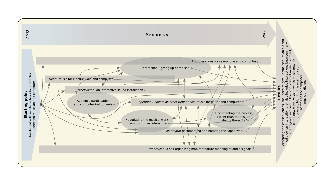
\includegraphics[width=\textwidth]{img/map8-noheader}
%   \caption{A timeline with the different sub-projects and themes with % their interrelations.}
%   \label{fig:main-map-ending}
% \end{figure}

%Accepting the consequences (the need to give up 'the Self') of an extended view on interaction that also includes interactions between many other agents involved in the production of musical content, led to new ways ways in which music may be produced, blurring the work concept as well as the composer-musician divide.

\begin{wrapfigure}{r}{0.24\linewidth}
\centering
\includegraphics[width=0.95\linewidth]{img/map8-results.png}
\end{wrapfigure}
Throughout this project I have tried to understand what it means to play with, on, and through computers, alone and with others. At the outset I could not have imagined that the idea of \emph{resisting control} would be the pivotal concept. In fact, I was convinced that Interactive Music was about \emph{gaining} control over the computer as a first step towards a more dynamic \useGlosentry{glos:musician}{musician}-\index{interaction!computer}computer interaction. With hindsight, of course, I can see that the dissociation from \index{interaction!as control}interaction-as-control had always been there. Neither could I have anticipated that a return to a more radical improvisatory attitude towards \emph{all} aspects of my musical practice would be one of the outcomes. Common to both of these concepts, the giving up of control, and the improvisatory attitude (which are not necessarily symmetrical; an improvisatory attitude does not inevitably resist control methodologies) is the notion of giving up the \index{Self}Self. To me, the reciprocity of \index{interaction!social}social interaction assumes that those engaged in the interaction unleash some part of their Selves or else the communication in the interaction would simply bounce off the unchangeable, morphous egos. Interaction should lead to some kind of change, it should induce a \emph{difference} (that makes a difference) and only if the \index{Self}Self is prepared to accept difference will this be possible.

The extended view on \index{interaction!human-computer}\index{HCI}human-computer interaction that I have presented here, along with the blurred work concept and a developed (i.e. different from Eco's definition) concept of \useGlosentry{glos:work_in_movement}{work-in-movement}, led to the need to explore the significance of giving up the \index{Self}Self.  At the same time, however, the processes launched by this project would not have reached the work-in-motion or \index{interaction!as difference}\index{interaction-as-difference}interaction-as-difference had I not already started to let go of the Self. But what part of the \index{Self}Self is to be abandoned? Is any part of the \index{Self}Self at all retractable? The point here is not to show that by deserting some part of subjectivity, another, `truer', unconscious identity hidden below, deeper down, is revealed. It is a common mistake, also produced by psycho-analysis itself, to believe that the Freudian unconscious would be served well by being disclosed, made conscious: ``The unconscious is understood as a negative, it's the enemy.''\footcites[][57]{deleuze77}[See also][128-56]{bateson72} The \index{Self}Self is not first and foremost given up to discover something \emph{within}, but to become more resonant to that by which it is surrounded. Then the innermost part of the \index{Self}Self, conscious or unconscious, will also be affected. Jacques \citeauthor{attali85} writes that when ``music ceases to be catharsis; it no longer constructs differences. \emph{It is trapped in identity and will dissolve into noise}''.\footcite[45]{attali85} Similarly, I would like to propose that unless the \index{Self}Self allows for \index{interaction!as difference}\index{interaction-as-difference}interaction-as-difference, allows for the Other to play an active part in the interaction, the \index{Self}Self will cease to produce difference as well as cease to apprehend difference and will be trapped in its own identity.

The idea of the \index{Self}Self as soluble in artistic practice and music in particular is not new, nor is it original.\footnote{Although the field of art activity appears to me to have produced more egos than it has dissolved.} To philosopher Julius T. \citeauthor{fraser90}, the way music (and dance) embraces all levels of temporality it in some cases leads to the ``loss of individuality and establishes timeless belonging''.\footcite[410-1]{fraser90} Just as Brandon \citeauthor{labelle06}, with reference to Robin Maconie, talks about how ``sound and the self are wrapped up together'',\footcite[62]{labelle06} multimedia artist Frances Dyson similarly points to the intermingling of sound and identity: ``sound at the same time destroys the possibility of distinguishing between subject and environment, self and other, interior and exterior. Immersed in sound, the subject thus loses its self''. Furthermore, \citeauthor{labelle06}'s book \citetitle{labelle06} is an historical overview of concepts related to the loss of the \index{Self}Self in the context of sound art, music, and architecture, starting with John Cage and proceeding to the present day. In particular is the discussion in Part 3 of the book, relating to the voice is interesting in the present context and in an analysis of Marina Abramovic's performance \emph{Freeing the Voice} (1975), \citeauthor{labelle06} writes that she ``enacts the dynamic of speech as being, in one and the same instant, a process of losing and regaining oneself---that is, a form of catharsis''.\footcite[103]{labelle06} \citeauthor{labelle06} also discusses Alvin \citeauthor{lucier69}'s brilliant 1969 piece of sound art \citetitle{lucier69}, which is perhaps one of the more palpable examples of loss of the \index{Self}Self in sound. The score for the piece consists of a written instruction to sit down in a room with a microphone, two tape recorders, an amplifier and speakers. To play the piece is to read the specified text and record it onto one of the tape recorders and then play it back into the room while recording it onto the second tape recorder, after which the newly-recorded version is played back and recorded, etc. The effect is that eventually the spoken words begin to deteriorate and the resonances of the room take over. The \index{Self}Self, as constituted by the voice, is completely decomposed and immersed in the room.

\index{interaction!as control}Interaction-as-control and \index{interaction!as difference}\index{interaction-as-difference}interaction-as-difference are not opposites. They are complementary concepts in the large domain of \index{interaction!human-computer}\index{HCI}human-computer interaction. As noted above, at the beginning of the project I was expecting to have to develop my skills in order to build tools for better and more precise control of the computer in order to let go of the control agency and start thinking about more dynamic agencies. This is along the lines of the common, Western, ideal of learning and knowledge; develop a skill and master it. Perfect the skill and avoid mistakes. Although traditional conservatory training functions along the same lines, in much artistic practice, and in improvisation in particular, the mistake is a fundamental agent, a source of inspiration not to be avoided.\footcite[See][148-60]{evens05} But a mistake occurs only if I allow it to happen and will go unnoticed if I lack the skill or the insight to realise it has happened. The mistake depends on skill. It too is a difference that I will fail to detect if I am unable to understand what was mistaken. In other words, a certain amount of control is necessary in order to give up control. And the balance between `control' and `lose control', between \index{Self}Self and giving up of the \index{Self}Self, is a deceitful one. The story narrated by John \citeauthor{corbett94} in his book \citetitle{corbett94} of how drummer Milford Graves manages to stop his heart from beating at will prior to playing a solo concert is perhaps one of the more radical examples of \emph{controlling} the loss of the \index{Self}Self.\footnote{Graves's solo playing in general is an excellent example of how the most intimate and detailed level of physical control is dissolved in what I perceive as the most incredible freedom.} What could be a more radical way of losing the \index{Self}Self than to stop one's heart at will?\footcite[74]{corbett94} The computer, however, is a phenomenal losing-control and forgetting machine, in this context a less lethal one. As remarked in many places throughout this text it increases resistance and introduces dualities and alternate personalities in a way that forces one to constantly relocate or give up the \index{Self}Self. It is similar to how Ornette Coleman's playing of the trumpet and the violin introduces resistance, forces Coleman to give up part of the skill he acquired on the saxophone; similar to how Marcel Duchamp used mechanical drawing in order to ``avoid the old-fashioned form of drawing'', to forget with his hand\footcite[Duchamp quoted in][29]{tomkins65} and how Paul D. \citeauthor{miller08} (DJ Spooky) uses turntables to forget: ``it seemed that turntables were somehow imbued with the art of being memory permutation machines. They changed how I remembered sounds and always made me think of a different experience with each listening''.\footcite[45]{miller04} It is my aim to continue to learn the computer, learn its languages and its methods, in order to forget and thus allow for novel experiences. Control (by learning I gain control) as an instrument also to lose control (by forgetting).

To resist control, then, is as much a posture as it is a different kind of (implementation of) \index{interaction!human-computer}\index{HCI}human-computer interaction and in this sense it is related to improvisation. Again, risking triggering an ideological debate on composition versus improvisation (see \hyperref[sec:personal-background]{Section \ref*{sec:personal-background}}), I believe there is a relation between these two musical practices somewhat similar to the relation between \index{interaction!as control}\index{interaction-as-control}interaction-as-control and \index{interaction!as difference}\index{interaction-as-difference}interaction-as-difference. On the one hand stands the ostensible sense of control that the finalised musical score, sometimes homologous to \emph{the work}, offers its composer in its flat surface representation of ``musical formalism [\ldots] entirely divorced from any relationship to intuitive gestural experience''.\footcite[35]{wis96} On the other hand stands the likewise apparent \emph{freedom} of musical improvisation which in some cases and under certain conditions is anything but formalised.\footnote{In other cases it is as formalised as any compositional practice.} Composition, and the printed score, as a means to gain control over one's own music, to make it tangible, archivable and sustainable. Improvisation as a practice to create differences that loses meaning outside the context against which the difference is created. But, once more, \index{interaction!as difference}\index{interaction-as-difference}interaction-as-difference is also an attitude. An attitude that can be applied to the practice of composition which is seen in \emph{Drive} and 
\emph{Repetition Repeats all other Repetitions}, and an attitude that may be supported by the technologies and ideas that have been developed within the framework of \emph{libIntegra}. 

%\begin{wrapfigure}{r}{0.45\linewidth}
  \begin{minipage}[h]{\linewidth}
    \begin{flushright}
      \musicannot{Drive\\
        \emph{for Electric Viola Grande and computer}\\
        Composed \& premiered in 2002\\
        Commissioned by and dedicated to Henrik Frendin}
    \end{flushright}
  \end{minipage}
\end{wrapfigure}

%%% Local Variables: 
%%% mode: latex
%%% TeX-master: "../ImprovisationComputersInteraction"
%%% End: 

Although I was yet unaware of it, the change was already noticeable in the earliest artistic sub-project, \emph{Drive}. In the interaction between Frendin and me the significance of the roles of composer and performer had already begun to wear off, but the sub-project that induced the \emph{difference} that made me aware of my unresolved need for control was \emph{etherSound}. After the initial excitement of having set everything up and experienced the installation working, I had to face the fear that I could not, in fact, fully control the output. First of all because it would be impossible to be physically present at all times: the installation would be active for three weeks, ten hours a day; second because the participants would have their own will and their own ideas of when and how to contribute. Even though the idea for \emph{etherSound} had come up in collaboration with the curator Miya Yoshida, I had programmed it myself. In other words, similarly to how it is described in \hyperlink{sec:target:overview-1}{the Introduction}, I as a detached \index{Self}Self did the programming of \emph{etherSound} and created a situation that I as the situated \index{Self}Self and as composer felt deeply uncomfortable with. In the interaction with my \index{Self}Self, mediated through the computer, a difference was induced thanks to which I learned the importance of giving up some part of that same \index{Self}Self. 

%\begin{wrapfigure}{r}{0.45\linewidth}
  \begin{minipage}[h]{\linewidth}
    \begin{flushright}
      \musicannot{Repetition Repeats all other Repetitions\\
        \emph{for ten-stringed guitar and computer}\\
        Composed \& premiered in 2006\\
        Commissioned by and dedicated to Stefan \"{O}stersj\"{o}}
    \end{flushright}
  \end{minipage}
\end{wrapfigure}

%%% Local Variables: 
%%% mode: latex
%%% TeX-master: "../ImprovisationComputersInteraction"
%%% End: 

Within \emph{Repetition Repeats all other Repetitions} the intellectual understanding of the phenomena I had already experienced began to take shape. In the collaboration between Stefan \"{O}stersj\"{o} and Love Mangs these aspects of interaction and the \index{Self}Self were seen in a new light. The understanding of composition as a negotiation, regardless of what level of interaction the composing is part of, paved the way for a different understanding of the practice of composition. It was, however, in the radical way that we gave up the notion of \emph{the work}, and even the \emph{open work} and established a re-interpretation of Eco's \emph{work-in-movement} that the full consequences of my altered composer role became evident. The \useGlosentry{glos:work_in_movement}{work-in-movement} is focused on the process rather than the result, in itself not a novel idea at all. In the context of computers and interaction and in combination with the idea of the augmented score, however, the focus on the process allowed an altered view on musical interpretation as well as composition: the score as a growing container of musical experience (rather than a detailed instruction to be rigorously followed), all of which is open-sourced to allow for any kind of transformation but with the request to let the interactive narrative, the collaboration, guide the additions, alterations and removals of material from the score.

%\begin{wrapfigure}{r}{0.4\linewidth}
  \begin{minipage}[h]{\linewidth}
    \begin{flushright}
      \musicannot{IntegraBrowser\\
        \emph{Offline browser for the Integra XML\\documentation format.}}
    \end{flushright}
  \end{minipage}
\end{wrapfigure}

%%% Local Variables: 
%%% mode: latex
%%% TeX-master: "../ImprovisationComputersInteraction"
%%% End: 

\emph{libIntegra} is the glue that potentially can make interaction simpler between environments for live \index{electro-acoustic music}electro-acoustic music. Not only is the augmented score enabled by aspects of libIntegra, but the fact that the \useGlosentry{glos:dsp}{DSP} modules, environments and stand-alone programs which may be described, shared and communicated in a uniform and abstract way are integral aspects of \emph{libIntegra} and furthers the idea of the \useGlosentry{glos:work_in_movement}{work-in-movement}. The core definitions of the protocol have been defined as openly as possible in order to allow for a widespread and distributed community to contribute to its expansion. 

These four mapped projects, \emph{Drive}, \emph{etherSound}, \emph{Repetition\ldots} and \emph{libIntegra} are framed by the improvisations and \emph{timbreMap} (see Figure \ref{fig:main-map}; by the most elusive and abstract (improvisation) and the most formal and concrete (programming). Now both of these are also in themselves representatives of the abstract-concrete opposition: improvising \emph{with} computer and a computer program that interacts with \emph{sound}. Improvisation, computer, sound. Integrated by interaction. Improvisation communicated to the computer, mediated by sound. The computer communicating with the improviser, mediated by sound. Sound as the interface. Since timbre (the quality of the sound/interface), can only be described in terms of \emph{difference} from other timbres surrounding it (leaving any theory of a general sound morphology aside),\footnote{Timbre, according to OED, is ``The character or quality of a musical or vocal sound (distinct from its pitch and intensity) [\ldots] distinguishing it from sounds proceeding from other sources'' \cite{timbre-oed}} the sound/interface is in itself a kind of difference: \index{interaction!as difference}\index{interaction-as-difference}interaction-as-difference. Furthermore, the map is a good visual representation of the function of time in the interactive system; it can even be seen as a graphic representation of the interaction between the different sub-projects. Time has been the topic in several sections, and the difference between parallel motion systems, systems that have some notion of time, however limited, and trigger-event systems, pure stimuli-response systems with no recollection of prior events, was discussed in \hyperref[sec:drive-2003]{Section \ref*{sec:drive-2003}}. This project is and has been a parallel motion system. The different sub-projects have informed each other but they have maintained their forward motion independently of each other in a way similar to how \emph{Drive} is portrayed in \hyperref[fig:parllel]{Figure \ref*{fig:parllel}}.

The six trajectories that took me from the starting-point to here, to the next beginning, have helped me better understand the concepts of interaction, openness, \index{Self}Self and control. But as containers they also hold some of the knowledge within them, and, owing to the intended open form and the fact that each of these projects can take off on its own, independent of my involvement and consent, whatever knowledge is encoded in them will then continue to develop. I propose an open-source music that is not only the \emph{grab-and-play} of P2P\footnote{Peer-to-peer networks are used widely for file sharing purposes.} and Bit Torrents but more of a distribution of construction kits. Build your own music. \citeauthor{corbett94}, leaning on Jacques Attali,\footcite[See][]{attali85} writes how ``improvising musicians create a genuine Deleuzian assemblage, a musical machine of desire---not binary, nor unitary, but multiple''.\footcite[76]{corbett94} Why should the musical assemblage be limited to improvising musicians? I am aiming at an even more decentralised assemblage (although it, too, will have to deal with limitations, for it is dependent on computers and networks). Central to the idea of the musical open-source is the reciprocity; what is taken is altered and returned and thus added to all other contributions. Each such bundle of musical practice that holds within it multiple relations and multiple kinds of interaction is a veritable work-in-movement, truly moving around in a way I am sure Eco did not anticipate.
\newpage
\thispagestyle{empty}

%But if it is not possible to control technology and it is not possible to give up technology, then our only choice is to stop \emph{trying} to control it and accept it as a, this time truly epistemological Other.

%%% Local Variables: 
%%% mode: latex
%%% TeX-master: "../ImprovisationComputersInteraction"
%%% End: 


% \printglossary
% \label{sec:gloss}

\nocite{oed89,ebonline09,oswald95}
\addcontentsline{toc}{chapter}{Bibliography}
\printbibliography[%
    notcategory=nobib
]
\label{sec:biblio}

\addcontentsline{toc}{chapter}{Index}
\printindex
\label{sec:index}

\end{document}